\scsection{Предметная область и онтология семантических моделей ostis-систем}

\scsubsection{\textbf{Предметная область и онтология внутреннего языка ostis-систем и близких ему внешних языков}}

\scsubsubsection{Предметная область и онтология внутреннего языка ostis-систем}
\label{sd_sc_code}
\input{Contents/chapter2/sd_ostis_sys_models/sd_sc_code.tex}

\scparagraph{Предметная область и онтология синтаксиса внутреннего языка ostis-систем}
\begin{SCn}

\scnsectionheader{\currentname}
\scnstartsubstruct

\scnheader{Предметная область синтаксиса SC-кода}
\scnsdmainclass{sc-элемент}
\scnsdclass{SC-код? \textbf{= sc-текст?};sc-узел;sc-коннектор;sc-дуга;sc-ребро;базовая sc-дуга;Алфавит SC-кода?}
\scnsdrelation{инцидентность sc-коннектора*;инцидентность входящей sc-дуги*}

\scnheader{SC-код}
\scnnote{Универсальность SC-кода позволяет с его помощью описывать любые объекты. Таким объектом может быть любой язык коммуникации с пользователями (в том числе и естественный язык), а также сам SC-код. Синтаксис и семантика SC-кода описываются в виде соответствующей формальных онтологий.}

\scnheader{sc-элемент}
\scnidtf{атомарный фрагмент хранимой в памяти знаковой конструкции, принадлежащей SC-коду}

\scnheader{Алфавит SC-кода}
\scneqtoset{sc-элемент;sc-узел;sc-коннектор;sc-дуга;sc-ребро;базовая sc-дуга}

\scnheader{sc-ребро}
\scnidtf{неориентированный sc-коннектор}
\scnheader{sc-дуга}
\scnidtf{ориентированный sc-коннектор}

\scnheader{Алфавит SC-кода}
\scnnote{В отличие от других языков, классы синтаксически выделяемых элементарных фрагментов текстов SC-кода могут пересекаться. Так, например, sc-элемент может одновременно принадлежать и классу \textit{sc-элементов} и классу \textit{sc-узлов}, а также может одновременно принадлежать и классу \textit{sc-элементов}, и классу \textit{sc-коннекторов}, и классу \textit{sc-дуг}, и классу \textit{базовых sc-дуг}.

Такая особенность \textit{Алфавита SC-кода} дает возможность строить синтаксически корректные \textit{\textbf{sc-тексты}} (тексты SC-кода) в условиях неполноты наших исходных знаний о некоторых \textit{sc-элементах}.}

\scnheader{sc-элемент}
\scnreltoset{разбиение}{sc-узел;sc-коннектор}
\scnheader{sc-коннектор}
\scnreltoset{разбиение}{sc-ребро;sc-дуга}
\scnheader{sc-дуга}
\scnsuperset{базовая sc-дуга}
\scnheader{инцидентность sc-коннектора*}
\scnrelfrom{первый домен}{sc-коннектор}
\scnrelfrom{второй домен}{sc-элемент}
\scnsuperset{инцидентность входящей sc-дуги*}
\scniselement{бинарное отношение}
\scniselement{ориентированное отношение}
\scniselement{отношение, среди элементов которого нет мультимножеств}
\scnaddlevel{1}
\scnnote{Для бинарных отношений принадлежность данному классу означает отсутствие петель}
\scnaddlevel{-1}
\scnheader{инцидентность входящей sc-дуги*}
\scnrelfrom{первый домен}{sc-дуга}
\scnrelfrom{второй домен}{sc-элемент}

\scnheader{sc-текст}
\scnnote{В процессе обработки \textbf{\textit{sc-текстов}} выполняются следующие правила уточнения их синтаксической разметки:
\begin{scnitemize}
    \item если стало известно, что \textit{sc-элемент}, имеющий метку \textit{sc-элемента}, является \textit{sc-узлом} или \textit{sc-коннектором}, то ему приписывается метка \textit{sc-узла} или  \textit{sc-коннектора}, а метка \textit{sc-элемента} удаляется;
    \item если стало известно, что \textit{sc-элемент}, имеющий метку \textit{sc-коннектора}, является \textit{sc-ребром} или \textit{sc-дугой}, то ему приписывается метка \textit{sc-ребра} или \textit{sc-дуги}, а метка \textit{sc-коннектора} удаляется;
    \item если стало известно, что \textit{sc-элемент}, имеющий метку \textit{sc-дуги}, является \textit{базовой sc-дугой}, то ему приписывается метка \textit{базовой sc-дуги}, а метка \textit{sc-дуги} удаляется.
\end{scnitemize}
}

\scnheader{SC-код}
\scntext{особенности}{Отметим некоторые синтаксические особенности SC-кода. 
\begin{scnitemize}
    \item Тексты SC-кода являются \textbf{абстрактными} в том смысле, что они абстрагируются от конкретного варианта их кодирования в памяти компьютерной системы. Кодирование текстов, в частности, зависит от варианта технической реализации памяти компьютерной системы. Так, например, актуальной является аппаратная реализация ассоциативной нелинейной памяти, в которой реализуется структурная реконфигурация хранимой информации, в которой обработка информации сводится не к изменению состояния элементов памяти, а к изменению конфигурации связей между ними.
    \item Тексты SC-кода являются структурами \textbf{графоподобного вида}. Все исследованные до настоящего времени графовые структуры легко представимы в SC-коде (неориентированные и ориентированные графы, мультиграфы, псевдографы, гиперграфы, сети и др.). Но, кроме этого, в SC-коде представимы и связи между связями, связи между целыми структурами и многое другое. SC-код фактически является \textbf{графовым языком}, текстами которого являются графоподобные структуры. Таким образом, теория графов при соответствующем ее расширении может стать основой описания синтаксиса SC-кода.
\end{scnitemize}

Простота синтаксиса \textit{\textbf{SC-кода}} обусловлена следующими \textbf{семантическими} свойствами \textit{sc-текстов} (знаковых конструкций, принадлежащих SC-коду).

\begin{scnitemize}
    \item \textbf{Все} (!) \textit{sc-элементы}, то есть элементарные (атомарные) фрагменты \textit{sc-текстов}, являются знаками (обозначениями) различных описываемых сущностей. При этом, каждая сущность, описываемая в тексте \textit{SC-кода}, должна быть представлена своим знаком;
    \item Никаких других знаков, кроме \textit{sc-элементов}, \textit{sc-тексты} не содержат (т. е. нет знаков, в состав которых входят другие знаки); 
    \item Любая сущность может быть описана \textit{sc-текстом} и, соответственно, представлена в этом \textit{sc-тексте} своим знаком;
    \item Все \textit{синтаксически выделяемые классы sc-элементов} (т.е. все элементы \textit{Алфавита SC-кода}) имеют четкую семантическую интерпретацию -- являются классами \textit{sc-элементов}, каждый из которых обозначает сущность, имеющую общие одинаковые свойства со всеми другими сущностями, обозначаемыми другими \textit{sc-элементами} этого же класса.
\end{scnitemize}}

\scnendstruct

\end{SCn}

\scparagraph{Предметная область и онтология базовой денотационной семантики внутреннего языка ostis-систем}
\begin{SCn}

\scnsectionheader{\currentname}

\scnstartsubstruct

\scnheader{Предметная область базовой денотационной семантики SC-кода}
\scnidtf{Предметная область сущностей}
\scnsdmainclasssingle{сущность}
\scnsdclass{...}

\scnheader{SC-код}
\scnexplanation{Денотационная семантика любой знаковой конструкции (в том числе и \textit{sc-текста}) с формальной точки зрения -- это соответствие (морфизм) между множеством всех знаков, входящих в знаковую конструкцию, и множеством денотатов этих знаков (т. е. сущностей, обозначаемых этими знаками), а также между множеством всех семантически значимых (семантически интерпретируемых) связей, связывающих знаки, и множеством соответствующих им связей, связывающих либо денотаты всех указанных знаков, либо денотаты некоторых из указанных знаков непосредственно с самими остальными знаками из числа указанных знаков.

Рассмотрим денотационную семантику \textit{sc-элементов}, принадлежащих разным \textit{синтаксически выделяемым классам sc-элементов}, т.е. имеющих разные синтаксические метки. 

Если \textit{sc-элемент}, имеет метку \textit{\textbf{sc-элемента}}, то он может обозначать \uline{любую} описываемую \textbf{сущность}. 

Если \textit{sc-элемент} имеет метку \textit{\textbf{sc-коннектора}}, который инцидентен \textit{sc-элементу} \textit{\textbf{ei}} и \textit{sc-элементу} \textit{\textbf{ej}}, то он, с одной стороны, является знаком \textit{\textbf{пары}} \{{\textit{\textbf{ei}}, \textit{\textbf{ej}}}\}, а, с другой стороны, является моделью (отражением, описанием) связи либо между денотатом \textit{sc-элемента} \textit{\textbf{ei}} и денотатом \textit{sc-элемента} \textit{\textbf{ej}}, либо между денотатом \textit{sc-элемента} \textit{\textbf{ei}} и самим \textit{sc-элементом} \textit{\textbf{ej}}, либо между денотатом \textit{sc-элемента} \textit{\textbf{ej}} и самим \textit{sc-элементом} \textbf{\textit{ei}}.

Если \textit{sc-элемент} имеет метку \textit{\textbf{sc-узла}}, то он обозначает \textbf{сущность, не являющуюся парой}.

Если \textit{sc-элемент} имеет метку \textit{\textbf{sc-ребра}}, которое инцидентно sc-элементу \textit{\textbf{ei}} и \textit{sc-элементу} \textit{\textbf{ej}}, то он, с одной стороны, является знаком \textit{\textbf{неориентированной пары}} \mbox{\{{\textit{\textbf{ei}}, \textit{\textbf{ei}}}\}}, а с другой стороны, является моделью (отражением, описанием) связи либо между денотатом \textit{sc-элемента} \textit{\textbf{ei}} и денотатом \textit{sc-элемента} \textit{\textbf{ej}}, либо между денотатом \textit{sc-элемента} \textit{\textbf{ei}} и самим \textit{sc-элементом} \textit{\textbf{ej}}, либо между денотатом \textit{sc-элемента} \textit{\textbf{ej}} и самим \textit{sc-элементом} \textit{\textbf{ei}}, либо непосредственно между самими \textit{sc-элементами} \textit{\textbf{ei}} и \textit{\textbf{ej}}.

Если \textit{sc-элемент} имеет метку \textbf{\textbf{sc-дуги}}, которая выходит из \textit{sc-элемента} \textit{\textbf{ei}} и входит в \textit{sc-элемент} \textit{\textbf{ej}}, то он, с одной стороны, является знаком \textit{\textbf{ориентированной пары}} \mbox{<\textit{\textbf{ei}}, \textit{\textbf{ej}}>}, а с другой стороны, является моделью (отражением, описанием) связи либо между денотатом \textit{sc-элемента} \textit{\textbf{ei}} и денотатом \textit{sc-элемента} \textit{\textbf{ej}}, либо между денотатом \textit{sc-элемента} \textit{\textbf{ei}} и самим \textit{sc-элементом} \textit{\textbf{ej}}, либо между денотатом \textit{sc-элемента} \textit{\textbf{ej}} и самим \textit{sc-элементом} \textit{\textbf{ei}}, либо непосредственно между самими sc-элементами \textit{\textbf{ei}} и \textit{\textbf{ej}}.

Если \textit{sc-элемент} имеет метку \textit{\textbf{базовой sc-дуги}}, которая выходит из \textit{sc-элемента} \textit{\textbf{ei}} и входит в \textit{sc-элемент} \textit{\textbf{ej}}, то он, с одной стороны, является знаком ориентированной \textit{\textbf{пары константной позитивной постоянной принадлежности}} <\textit{\textbf{ei}}, \textit{\textbf{ej}}>, а, с другой стороны, является моделью (отражением, описанием) связи между множеством, которое обозначается \textit{sc-элементом} \textit{\textbf{ei}}, и \textit{sc-элементом} \textit{\textbf{ej}}, который является одним из элементов указанного множества.

Теперь перейдем к рассмотрению денотационной семантики пар \textit{\textbf{инцидентности}} \textit{\textbf{sc-коннек-торов}}. Напомним, что каждый \textit{sc-коннектор} семантически трактуется как знак \textit{\textbf{пары}} \textit{sc-элементов}, инцидентных этому \textit{sc-коннектору}. Соответственно этому каждая \textit{пара инцидентности sc-коннектора}, \uline{не являясь sc-элементом}, семантически трактуется как модель (отражение, описание) связи между \textit{парой} sc-элементов, обозначаемой этим \textit{sc-коннектором}, и одним из двух элементов этой \textit{пары}. При этом принадлежность указанного \textit{sc-элемента} указанной \textit{паре} может носить:

\begin{scnitemize}
    \item \textit{\textbf{константный}} либо \textit{\textbf{переменный}} характер в зависимости от константности или переменности указанного \textit{sc-коннектора};
    \item \textit{\textbf{стационарный}} (постоянный) либо \textit{\textbf{нестационарный}} (ситуативный) характер в зависимости от стационарности или нестационарности указанного \textit{sc-коннектора}.
\end{scnitemize}

Аналогичным образом задается денотационная семантика пар \textit{\textbf{инцидентности входящих sc-дуг}}. Каждая такая пара инцидентности трактуется как модель связи между \textbf{\textit{ориентированной парой}}, обозначаемой \textit{sc-дугой} и вторым компонентом этой пары (т.е. \textit{sc-элементом}, в которой \textit{sc-дуга} входит). И аналогично парам \textit{инцидентности sc-коннекторов} пары \textit{инцидентности входящих sc-дуг} могут иметь \textit{константный} и \textit{переменный} характер, а также \textit{стационарный} и \textit{нестационарный} в зависимости от характера соответствующей \textit{sc-дуги}.

Формальное описание денотационной семантики \textit{SC-кода} средствами самого \textit{SC-кода} осуществляется в виде иерархической системы \textbf{\textit{формальных онтологий}} верхнего уровня, представленных в виде текстов \textit{SC-кода}. В базе знаний \textit{\textbf{Метасистемы IMS.ostis}} все эти онтологии представлены~\cite{IMS}.
}

\scnheader{сущность}
\scnidtf{sc-элемент}
\scnsubdividing{sc-константа;sc-переменная\\
\scnaddlevel{1} 
\scnidtf{знак произвольной сущности из некоторого множества возможных значений}
\scnaddlevel{-1}}

\scnsubdividing{стационарная сущность\\
\scnaddlevel{1} 
\scnidtf{постоянная сущность}
\scnaddlevel{-1} 
;sc-переменная\\
\scnaddlevel{1} 
\scnidtf{нестационарная сущность}
\scnidtf{сущность, изменяющаяся во времени}
\scnsuperset{временная сущность}
\scnaddlevel{1} 
\scnidtf{временно существующая сущность}
\scnaddlevel{-2} }

\scnsubdividing{материальная сущность;терминальная абстрактная сущность;файл\\
\scnaddlevel{1}
\scnaddhind{-1}
\scnidtf{первичный (при восприятии) или конечный (при отображении) электронный образ внешней информационной конструкции}
\scnaddlevel{-1} 
;множество\\
\scnaddlevel{1}
\scnidtf{множество sc-элементов}
\scnsubdividing{связь;структура;класс\\
\scnaddlevel{1}
\scnsubdividing{класс терминальных сущностей;отношение\\
\scnaddlevel{1}
\scnidtf{класс связей}
\scnaddlevel{-1}
;класс классов\\
\scnaddlevel{1}
\scnsuperset{параметр}
\scnaddlevel{-1}
;класс структур}
\scnaddlevel{-1}
}
\scnaddlevel{-1}
}

\scnheader{связь}
\scnidtf{связка}
\scnsubdividing{пара\\
\scnaddlevel{1}
\scnidtf{бинарная связь}
\scnsuperset{sc-коннектор}
\scnaddlevel{1}
\scnnote{Некоторые пары sc-элементов в некоторые периоды времени могут быть не оформлены синтаксически как коннекторы, но такое преобразование обязательно происходит.}
\scnaddlevel{-2}
;небинарная связь}

\scnsubdividing{неориентированная связь\\
\scnaddlevel{1}
\scnsuperset{неориентированная пара}
\scnaddlevel{-1}
;ориентированная связь\\
\scnaddlevel{1}
\scnsuperset{ориентированная пара}
\scnaddlevel{-1}
}

\scnsubdividing{константная связь\\
\scnaddlevel{1}
\scneq{(связь $\cap$ sc-константа)}
\scnaddlevel{-1}
;переменная связь\\
\scnaddlevel{1}
\scneq{(связь $\cap$ sc-переменная)}
\scnsuperset{sc-переменная, значениями которой являются константные связи}
\scnsuperset{sc-переменная, значениями которой являются переменные связи}
\scnaddlevel{-1}
}

\scnheader{пара}
\scnidtf{обозначение двухмощного множества sc-элементов}
\scnsubdividing{неориентированная пара\\
\scnaddlevel{1}
\scnsuperset{sc-ребро}
\scnaddlevel{-1}
;ориентированная пара\\
\scnaddlevel{1}
\scnsuperset{sc-дуга}
\scnsuperset{пара принадлежности}
\scnaddlevel{-1}
}
\scnsubdividing{пара-петля\\
\scnaddlevel{1}
\scnidtf{пара, являющаяся петлей}
\scnidtf{пара, у которой инцидентные ей sc-элементы совпадают}
\scnidtf{пара, являющаяся мультимножеством}
\scnaddlevel{-1}
;пара, не являющаяся петлей}

\scnheader{пара принадлежности}
\addtocounter{hind}{1}
\scnidtf{связь, описывающая характер принадлежности некоторого sc-элемента некоторому множеству}
\addtocounter{hind}{-1}
\scnsubdividing{пара константной принадлежности\\
\scnaddlevel{1}
\scneq{(пара принадлежности $\cap$ sc-константа)}
\scnaddlevel{-1}
;пара переменной принадлежности\\
\scnaddlevel{1}
\scneq{(пара принадлежности $\cap$ sc-переменная)}
\scnaddlevel{-1}
}
\scnsubdividing{пара постоянной принадлежности\\
\scnaddlevel{1}
\scneq{(пара принадлежности $\cap$ стационарная сущность)} 
\scnidtf{пара стационарной принадлежности} 
\scnaddlevel{-1}
;пара временной принадлежности\\
\scnaddlevel{1}
\scneq{(пара принадлежности $\cap$ временная сущность)} 
\scnidtf{пара ситуативной принадлежности}
\scnaddlevel{-1}
}
\scnsubdividing{пара позитивной принадлежности\\
\scnaddlevel{1}
\scnidtf{пара действительной принадлежности} 
\scnaddlevel{-1}
;пара нечеткой принадлежности;
пара негативной принадлежности\\
\scnaddlevel{1}
\scnidtf{пара несуществующей принадлежности} 
\scnaddlevel{-1}
}

\scnsuperset{пара константной позитивной постоянной принадлежности}
\scnaddlevel{1}
\scneq{(пара позитивной принадлежности $\cap$ sc-константа $\cap$ стационарная сущность)}
\scnsuperset{базовая sc-дуга}
\scnaddlevel{-1}

\scnendstruct

\scnsourcecomment{Завершили представление фрагмента Предметной области базовой денотационной семантики SC-кода}

\end{SCn}

\begin{SCn}
\scnsectionheader{\currentname}
\scnsuperset{Онтология сущностей}
\scnaddlevel{1}
\scntext{детализация}{Нижеперечисленные онтологии уточняют (детализируют) понятия, введенные в \textit{\textbf{Онтологии сущностей}}.

В \textit{\textbf{Онтологии множеств}} (см. Раздел \textit{\nameref{sd_sets}}) уточняется понятие \textit{множества} sc-элементов, рассматриваются различные классы множеств (конечные, бесконечные, счетные, континуальные, мультимножества, множества без кратных элементов), различные свойства (характеристики) и отношения, заданные на множествах (мощность множеств, включение, объединение, разбиение, пересечение и т.д.).

В \textit{\textbf{Онтологии отношений}} (см. Раздел \textit{\nameref{sd_rels}}) рассматриваются такие понятия, как \textit{бинарное отношение, унарное отношение, тернарное отношение, класс связок одинаковой мощности, класс связок разной мощности, арность отношения, ориентированное, неориентированное отношение, ролевое отношение, атрибут отношения*, область определения отношения*, домен отношения по заданному атрибуту*, функция}, и т.д.

Для \textit{Онтологии отношений} вводится онтология более низкого уровня -- \textit{\textbf{Онтология бинарных отношений и соответствий}}, которая наследует все свойства отношений, описанных в \textit{Онтологии отношений}, уточняет понятие \textit{бинарного отношения} И рассматривает такие понятия, как \textit{транзитивное отношение, симметричное отношение, рефлексивное отношение, отношение эквивалентности, изоморфизм, гомоморфизм} и т.д.

Далее вводятся 
\begin{scnitemize}
    \item \textbf{\textit{Онтология параметров, величин и измерений}} (см. Раздел \textit{\nameref{sd_params}}) 
    \item \textbf{\textit{Онтология структур}} (см. Раздел \textit{\nameref{sd_structures}})
    \begin{scnitemizeii}
    \item \textit{\textbf{Онтология предметных областей}} (см. Раздел \textit{\nameref{sd_sd}})
    \item \textit{\textbf{Онтология семантических окрестностей}} (см. Раздел \textit{\nameref{sd_sem_neigh}})
    \item \textit{\textbf{Онтология баз знаний}} (см. Раздел \textit{\nameref{sd_kb}})
    \end{scnitemizeii} 
    \item \textit{\textbf{Онтология логических формул}} (см. Раздел \textit{\nameref{sd_logics}})
    \item \textit{\textbf{Онтология темпоральных сущностей}}, в которой рассматриваются такие понятия, как \textit{нестационарный параметр} (состояние), \textit{процесс, действие, ситуация, последовательность во времени*, темпоральная декомпозиция*} и др. (см. Раздел \textit{\nameref{sd_temp_entities}})
    \begin{scnitemizeii}
    \item \textbf{\textit{Онтология действий, задач, планов, протоколов и методов}} (см. Раздел \textit{\nameref{sd_actions}})
    \end{scnitemizeii}
    \item \textit{\textbf{Онтология внешних информационных конструкций}} (см. Раздел \textit{\nameref{sd_files}})
\end{scnitemize}


Некоторые из \textit{онтологий}, представленных в \textit{SC-коде}, носят "общеобразовательный"\ характер. Это означает, что для качественного взаимопонимания между любыми субъектами (как пользователями, так и компьютерными системами), т.е. для качественной их семантической совместимости все эти "общеобразовательные"\ онтологии, причем в согласованном, унифицированном виде, должны знать \uline{все}(!). Иначе никакого взаимопонимания не будет.

Список \textit{онтологий} можно продолжать. Все \textit{онтологии} постоянно меняются (уточняются, совершенствуются). Важнейшим критерием качества иерархической системы \textit{онтологий} является стратифицированность способов решения задач, соответствующих различным \textit{онтологиям} -- для каждой решаемой задачи желательно априори знать, в рамках какой \textit{онтологии} она может быть решена.

Очевидно, что, кроме "общеобразовательных"\ \textit{онтологий} существует большое число профессиональных, специализированных \textit{онтологий}, согласованное представление и знание которых необходимо для взаимопонимания (совместимости) всех тех, кто работает в соответствующей профессиональной области. 

Таким образом, денотационная семантика \textit{SC-кода}, как и любого другого языка, претендующего на универсальность, отражает текущее состояние наших знаний и, следовательно, может изменяться. Очевидно, что наиболее интенсивно эти изменения происходят в специализированных и новых областях знаний.
}
\scnaddlevel{-1}

\end{SCn}

\scsubsubsectionfinish{sd_sc_code}
\begin{SCn}

\scnsectionheader{\nameref{sd_sc_code}}

\scnstartsubstruct

\scnheader{sc-модель семантической совместимости}
\scnexplanation{Важнейшим этапом эволюции любой технологии является переход к \textbf{компонентному проектированию} на основе постоянно пополняемый \textbf{библиотеки многократно используемых компонентов}.

Основной проблемой для реализации компонентного проектирования являются 
\begin{scnitemize}
    \item унификация компонентов по форме; 
    \item разработка стандартов обеспечивающих совместимость этих компонентов.
\end{scnitemize}

Для реализации компонентного проектирования \textit{базы знаний} требуется:

\begin{scnitemize}
    \item универсальный язык представления знаний;
    \item универсальная процедура интеграции знаний в рамках указанного языка; 
    \item разработка стандарта, обеспечивающего \textbf{семантическую совместимость} интегрируемых знаний (таким стандартом является согласованная система используемых понятий).
\end{scnitemize}

Даже для смыслового представления знаний нужны, своего рода, смысловые семантические координаты, роль которых выполняет используемая система понятий (своего рода, ключевых знаков), которая, в свою очередь, описывается (специфицируется, задается) иерархической системой семантически связанных между собой \textit{онтологий}.

Другими словами, человеческие знания необходимо привести к общему "семантическому знаменателю"\ (к общей семантической системе координат), чем является постоянно уточняемая система понятий, специфицируемая в виде объединенной онтологии. Эта объединенная онтология \textbf{стратифицируется} на частные онтологии, эволюционируемые в достаточной степени \textbf{независимо} друг от друга.

Одним из критериев семантической совместимости новой информации с базой знаний, в которую эта информация погружается, можно сформулировать следующим образом. 

Все знаки, являющиеся новыми для воспринимающей базы знаний (в которую погружаются эти новые знаки) должны быть в достаточной степени специфицированы (а для новых понятий -- определены) через понятия, известные базе знаний.

Стандарт смыслового представления информации (\textit{SC-код}) дает возможность, с одной стороны, повысить уровень совместимости компьютерных систем, а с другой стороны, формально уточнить понятие интеграции компьютерных систем и их компонентов. 

При этом следует отличать: 
\begin{scnitemize}
    \item Cемантическую интеграцию двух текстов, принадлежащих языку смыслового представления информации (SC-коду). В результате такой интеграции два исходных sc-текста преобразуются в один интегрированный текст;
    \item Семантическую интеграцию двух разных моделей обработки информации, представленной в SC-коде;
    \item Модель понимания текста некоторого внешнего языка путем трансляции исходного внешнего текста в SC-код и последующbм погружением построенного sc-текста в базу знаний, представленную в SC-коде.
    \item Семантическую интеграцию двух компьютерных систем, построенных на основе SC-кода;
    \item Семантическую совместимость компьютерной системы, построенной на основе SC-кода, с ее пользователями.
\end{scnitemize}
}

\scnendstruct

\end{SCn}

\scsubsubsection{Предметная область и онтология внешних идентификаторов знаков, входящих в состав текстов внутреннего языка ostis-систем}
\begin{SCn}

\scnsectionheader{\currentname}
\scntext{эпиграф}{Если вещи будут именоваться неправильно, слова потеряют силу и ни одно дело нельзя будет довести до конца. Конфуций 5-6 вв. до н.э.}
\scntext{эпиграф}{Удачно выбранный термин – путь к пониманию и признанию, а неудачно выбранный – путь к забвению.}

\scnstartsubstruct

\scnheader{Предметная область внешних идентификаторов sc-элементов}
\scniselement{предметная область}
\scnsdmainclasssingle{идентификатор}
\scnsdclass{строковый идентификатор;нестроковый идентификатор;атомарный идентификатор;неатомарный идентификатор;идентификатор-контур;идентификатор-файл;идентификатор-множество;идентификатор-кортеж;идентификатор-операция;системный идентификатор}
\scnsdrelation{идентификатор*;основной идентификатор*;системный идентификатор*;последовательность внешних идентификаторов*}

\scnheader{идентификатор}
\scnidtf{sc-знак внешнего идентификатора некоторого sc-элемента}
\scnidtf{внешний идентификатор sc-элемента}
\scnidtf{sc-знак sc-идентификатора}
\scnrelto{второй домен}{идентификатор}
\scnsubset{файл}
\scnexplanation{Под \textbf{\textit{идентификатором}} понимается файл, который может быть использован для обозначения (именования) той или иной сущности в рамках какого-либо \textit{внешнего языка}. \textbf{\textit{Идентификатором}} может быть, в том числе, \textit{изображение}.

Существенно подчеркнуть, что выбор \textit{идентификаторов} влияет только на первичное восприятие принимаемых сообщений и на конечный этап синтеза передаваемых сообщений, но никак не влияет на рассуждения.

Другими словами, \textbf{\textit{идентификатор}} это \textit{sc-знак файла}, в котором хранится в определенном формате электронный образ одного из экземпляров класса синтаксически эквивалентных конструкций, все или многие из которых, входя во внешние тексты, обозначают ту же сущность, что и соответствующий им \textit{sc-элемент}.}
\scnsubdividing{строковый идентификатор;нестроковый идентификатор}

\scnheader{строковый идентификатор}
\scnexplanation{Наиболее часто используемыми \textit{идентификаторами} являются \textbf{\textit{строковые идентификаторы}}, которые представляют собой строку символов какого-либо фиксированного алфавита.}
\scnsubdividing{атомарный идентификатор;неатомарный идентификатор}

\scnheader{нестроковый идентификатор}
\scntext{примечание}{Помимо \textit{строковых идентификаторов}, выделяются \textbf{\textit{нестроковые идентификаторы}}, которые идентифицируют объекты при помощи графических иллюстраций, символов, иероглифов, пиктограмм и др.}

\scnheader{атомарный идентификатор}
\scntext{примечание}{\textbf{\textit{атомарный идентификатор}} - это \textit{идентификатор}, при формировании которого не используются другие \textit{идентификаторы}.}
\scnhaselementrole{пример}{\textnormal{[треугольник]}}

\scnheader{неатомарный идентификатор}
\scntext{примечание}{\textbf{\textit{неатомарный идентификатор}} - это \textit{идентификатор}, в состав которого входят другие \textit{идентификаторы}.}
\scnhaselementrole{пример}{
\textnormal{[Треугк.(Тчк.А; Тчк.B; Тчк.С)]}\\
\scntext{комментарий}{Приведен пример \textit{неатомарного идентификатора} - \textit{идентификатор} треугольника АВС. В своем составе данный \textit{идентификатор} содержит \textit{атомарные идентификаторы} трех точек, задающих этот треугольник: точка А, точка B и точка C.}}
\scnsuperset{идентификатор-контур}
\scnsuperset{идентификатор-ссылка}
\scnsuperset{идентификатор-множество}
\scnsuperset{идентификатор-кортеж}
\scnsuperset{идентификатор-операция}

\scnheader{идентификатор-контур}
\scnidtf{[* *]-идентификатор}
\scnexplanation{\textbf{\textit{идентификатор-контур}} - \textit{идентификатор sc-элемента}, который обозначает семантически эквивалентную \textit{структуру} для текста в скобках со звездочками, записанного на некотором внешнем языке, т.е. результат трансляции текста в скобках в \textit{SC-код}.}

\scnheader{идентификатор-файл}
\scnidtf{[ ]-идентификатор}
\scnidtf{идентификатор-рамка}
\scnexplanation{\textbf{\textit{идентификатор-файл}} представляет собой \textit{идентификатор sc-элемента}, который является \textit{файлом}, содержимым которого является некоторый текст в квадратных скобках, записанный на каком-либо \textit{внешнем языке}.}

\scnheader{идентификатор-множество}
\scnidtf{\{ \}-идентификатор}
\scnexplanation{\textbf{\textit{идентификатор-множество}} представляет собой \textit{идентификатор sc-элемента}, являющегося \textit{множеством}, которому принадлежат элементы, \textit{идентификаторы} которых перечисляются в фигурных скобках через знак точки с запятой «;».

В скобках должны быть перечислены все элементы идентифицируемого \textit{множества}. Если перечисляются не все элементы идентифицированного \textit{множества}, то после последнего элемента ставится знак «;», а далее ставится знак «…».}
\scnrelfrom{типичная семантическая окрестность}{
\scnfilescg{figures/sd_identifiers/typical_sc_neighborhood_for_sc_identifier_set.png}}


\scnheader{идентификатор-кортеж}
\scnidtf{< >-идентификатор}
\scnexplanation{\textbf{\textit{идентификатор-кортеж}} – это \textit{идентификатор ориентированного множества}, которому принадлежат элементы, идентификаторы которых перечислены в скобках через знак точки с запятой «;». При этом считается, что всем элементам описываемого \textit{множества} приписаны \textit{числовые атрибуты}, соответствующие порядку следования имени элемента в перечислении.}
\scnrelfrom{типичная семантическая окрестность}{
\scnfilescg{figures/sd_identifiers/typical_sc_neighborhood_for_sc_identifier_tuple_set.png}}

\scnheader{идентификатор-операция}
\scnidtf{(+)-идентификатор}
\scnexplanation{\textbf{\textit{идентификатор-операция}} – это \textit{идентификатор sc-элемента}, являющегося результатом \textit{арифметической}, теоретико-множественной или \textit{логической операции}, обозначение которой записано какими-либо специальными символами в круглых скобках.}
\scnrelfrom{типичная семантическая окрестность}{
\scnfilescg{figures/sd_identifiers/typical_sc_neighborhood_for_sc_identifier_operation_set.png}}

\scnheader{идентификатор*}
\scniselement{бинарное отношение}
\scniselement{ориентированное отношение}
\scnexplanation{\textbf{\textit{идентификатор*}}- это бинарное \textit{ориентированное отношение}, связывающее \textit{sc-элемент} с \textit{файлом}, содержащим его идентификатор на каком-либо \textit{внешнем языке}.}

\scnheader{основной идентификатор*}
\scnsubset{идентификатор*}
\scnexplanation{\textbf{\textit{основной идентификатор*}}- это бинарное \textit{ориентированное отношение}, связывающее sc-элемент с \textit{файлом}, содержащим его основной идентификатор, т.е. \textit{идентификатор}, который должен быть уникален в рамках одного \textit{внешнего языка}.}

\scnheader{системный идентификатор*}
\scnsubset{идентификатор*}
\scnexplanation{\textbf{\textit{системный идентификатор*}}- это бинарное \textit{ориентированное отношение}, связывающее \textit{sc-элемент} с \textit{файлом}, содержащим его \textit{системный идентификатор}.}

\scnheader{системный идентификатор}
\scnidtf{глобальный идентификатор}
\scnsubset{идентификатор}
\scnrelto{второй домен}{системный идентификатор}
\scnexplanation{\textbf{\textit{системный идентификатор}} - это \textit{идентификатор}, являющийся уникальным в рамках всей \textit{базы знаний}. Данный \textit{идентификатор}, как правило, используется в исходных текстах базы знаний нижнего уровня. Для обеспечения интернационализации рекомендуется записывать \textbf{\textit{системные идентификаторы}} на английском языке.

Символами, использующимися в \textbf{\textit{системном идентификаторе}}, могут быть буквы латинского алфавита, цифры, знак нижнего подчеркивания и знак тире. 

Таким образом, наиболее целесообразно формировать \textbf{\textit{системный идентификатор}} \textit{sc-элемента} из основного англоязычного путем замены всех символов, не входящих в описанный выше алфавит на символ «\_».

Например:\\
основной англоязычный идентификатор: Partition. SCs-code. Dividers\\
\textbf{\textit{системный идентификатор}}: Partition\_SCs-code\_Dividers\\
Для именования \textit{sc-элементов}, являющихся знаками \textit{ролевых отношений}, вместо знака «’» в \textbf{\textit{системном идентификаторе}} используется приставка «rrel» и далее после нижнего подчеркивания записывается имя \textit{ролевого отношения}.\\
Для именования \textit{sc-элементов}, являющихся знаками \textit{неролевых отношений}, вместо знака «*» в \textit{системном идентификаторе} используется приставка «nrel» и далее после нижнего подчеркивания записывается имя \textit{неролевого отношения}.\\
Для именования \textit{sc-элементов}, являющихся знаками \textit{классов} понятий в идентификаторе используется приставка «concept» и далее после нижнего подчеркивания записывается имя \textit{класса}.\\
Для именования \textit{sc-элементов}, являющихся знаками \textit{структур} в идентификаторе используется приставка «struct» и далее после нижнего подчеркивания записывается имя \textit{структуры}.\\
Для именования \textit{sc-элементов}, являющихся знаками \textit{кортежей} в идентификаторе используется приставка «tuple» и далее после нижнего подчеркивания записывается имя \textit{кортежа}.

Например:\\
rrel\_summand\\
/*ролевое отношение «слагаемое’»*/\\
nrel\_inclusion\\
/*неролевое отношение «включение*»*/\\
concept\_triangle\\
/*класс «треугольник»*/\\
struct\_Triangle\_A\_B\_C\\
/*структура «Треугк(ТчкA;ТчкB;ТчкC)»*/
}

\scnheader{последовательность внешних идентификаторов*}
\scniselement{отношение строгого порядка}
\scnexplanation{\textbf{\textit{последовательность внешних идентификаторов*}} - это бинарное \textit{ориентированное отношение}, связывающее между собой связки отношения \textit{идентификатор*}, имеющие общий первый компонент, и упорядочивающее таким образом идентификаторы одного объекта между собой по некоторому критерию. Чаще всего таким критерием является степень ассоциируемости того или иного идентификатора с описываемым понятием, его «узнаваемость», «точность» и т.д.}

\scnendstruct

\end{SCn}

\scsubsubsection{Предметная область и онтология внешнего языка графического представления знаний ostis-систем}
\scparagraph{Предметная область и онтология синтаксиса внешнего языка графического представления знаний ostis-систем}
\scparagraph{Предметная область и онтология денотационной семантики внешнего языка графического представления знаний ostis-систем}

\scsubsubsection{Предметная область и онтология внешнего языка линейного представления знаний ostis-систем}
\begin{SCn}

\scnsectionheader{Предметная область и онтология SCs-кода}

\scnstartsubstruct

\scnheader{Предметная область SCs-кода}
\scnsdmainclasssingle{SCs-код}
\scnsdclass{***}
\scnsdrelation{***}

\scnheader{SCs-код}
\scnidtf{Semantic Code string}
\scnexplanation{SCs-код - строковый (линейный) вариант представления SC-кода. Предназначен для представления sc-графов (текстов SC-кода) в виде последовательностей символов, которые могут быть отредактированы как при помощи стандартных текстовых редакторов, так и при помощи специализированного sc.s-редактора. Следовательно, одним из требований, предъявляемых к SCs-коду, помимо полноты и непротиворечивости, является возможность набора исходных текстов без помощи специализированного редактора, используя только символы стандартной клавиатуры. В отличие от SCn-кода, также являющегося текстовым вариантом отображения sc-графов, в SCs-коде форматирование не имеет значения, все предложения могут быть записаны в одну строку.

В отличие от SCg-кода, в SCs-коде нет специальных обозначений для указания структурных типов sc-узлов, однако есть изображения sc-коннекторов, соответствующие ядру и расширению SCg-кода, а также изображения sc-коннекторов специального типа, для которых нет соответствия в SCg-коде. С формальной точки зрения SCs-код - множество sc.s-текстов. Каждый sc.s-текст представляет собой последовательность sc.s-предложений, каждое из которых оканчивается разделителем ;; (двойная точка с запятой). Множество sc.s-предложений разбивается на множество простых и множество сложных sc.s-предложений. Каждое сложное sc.s-предложение содержит в своем составе встроенные предложения, ограниченные ограничителем (*...*).

В рамках sc.s-текста любого уровня допустимо использование комментариев следующего вида:

// однострочный комментарий

/* многострочный комментарий */ 

В начале файла, содержащего sc.s-текст настоятельно рекомендуется указывать уровень и версию используемого SCs-кода. 
Для этого используются комментарий специального вида:
/* SCs\_code\textless" версия "\textgreater.Level\textless" номер уровня "\textgreater*/

Например:

/* SCs\_code0.1.0.Level 6 */

Следует отметить, что комментарий вида /*…*/, использованный внутри sc.s-рамки (см. соотв. раздел) не опускается при разборе sc.s-текста, и становится частью содержимого соответствующей sc-ссылки. Например при разборе предложения

X => r1: [TEXT1/*COMMENT*/TEXT2];;

Будет создана sc-ссылка с содержимым TEXT1/*COMMENT*/TEXT2, а не TEXT1TEXT2.

В SCs-коде условно выделяются 7 расширений. Все расширения равнозначны по возможностям представления знаний, однако расширения более высоких уровней описывают sc-графы более лаконично и удобно. Введение расширений призвано облегчить работу разработчиков баз знаний при наборе sc.s-текстов.
}

\scnheader{sc.s-предложение}
\scnsubdividing{простое sc.s-предложение\\
\scnaddlevel{1}
\scnidtf{sc.s-предложение, не содержащее встроенных sc.s-предложений}
\scnaddlevel{-1}
;сложное sc.s-предложение\\
\scnaddlevel{1}
\scnidtf{sc.s-предложение, содержащее встроенные sc.s-предложения}
\scnaddlevel{-1}}
\scnsubdividing{sc.s-предложение уровня 1;sc.s-предложение уровня 2;sc.s-предложение уровня 3;sc.s-предложение уровня 4;sc.s-предложение уровня 5;sc.s-предложение уровня 6;sc.s-предложение уровня 7}

\scnheader{sc.s-предложение уровня 1}
\scnexplanation{sc.s-предложение уровня 1 - sc.s-предложение, содержащее только sc.s-разделители инцидентности и имена sc-элементов.}
\scntext{пример}{включение* | sc-arc-main\#arc2 | sc\_arc\_common\#pair1;;}
\scntext{пример}{Четырехугк(ТчкА;ТчкВ;ТчкС;ТчкD) | sc\_arc\_common\#pair1 | Отр(ТчкВ;ТчкС);;}

\scnheader{sc.s-предложение уровня 2}
\scntext{пример}{сторона* $\ni$ (Четырехугк(ТчкА;ТчкВ;ТчкС;ТчкD) =\textgreater~Отр(ТчкВ;ТчкС) );;}
\scntext{пример}{включение* $\ni$ ( Треугк(ТчкВ;ТчкС;ТчкD) =\textgreater~Отр(ТчкВ;ТчкС) );;}

\scnheader{sc.s-предложение уровня 3}
\scntext{пример}{Четырехугк(ТчкА;ТчкВ;ТчкС;ТчкD) =\textgreater~ сторона* : Отр(ТчкВ;ТчкС);;}
\scntext{пример}{треугольник =\textgreater идентификатор* : основной англоязычный идентификатор*: [triangle];;}

\scnheader{sc.s-предложение уровня 4}
\scncomment{sc.s-предложение уровня 4 можно считать описанием семантической окрестности радиуса 1 для заданного sc-элемента, т.е описанием известных связей заданного sc-элемента с другими смежными ему sc-элементами.}
\scntext{пример}{Четырехугк(ТчкА;ТчкВ;ТчкС;ТчкD) =\textgreater~ сторона*: включение*: Отр(ТчкВ;ТчкС);\\ Отр(ТчкС;ТчкD);;}


\scnendstruct

\end{SCn}
\scparagraph{Предметная область и онтология синтаксиса внешнего языка линейного представления знаний ostis-систем}
\scparagraph{Предметная область и онтология денотационной семантики внешнего языка линейного представления знаний ostis-систем}

\scsubsubsection{Предметная область и онтология внешнего языка структурированного представления знаний ostis-систем}
\label{section_scn}

\scparagraph{Предметная область и онтология синтаксиса внешнего языка структурированного представления знаний ostis-систем}
\scparagraph{Предметная область и онтология денотационной семантики внешнего языка структурированного представления знаний ostis-систем}

\scsubsection{\textbf{Предметная область и онтология баз знаний ostis-систем}}
\label{sec:sd_kb}

\scsubsubsection{Предметная область и онтология знаний}
\begin{SCn}

\scnsectionheader{\currentname}

\scnstartsubstruct

\scnheader{Предметная область знаний и баз знаний ostis-систем}
\scniselement{предметная область}
\scnsdmainclasssingle{знание}
\scnsdclass{раздел;раздел-обоснование;раздел-документация;раздел-описание предметной области;раздел-описание семантической окрестности;раздел-описание принципов;неатомарный раздел;атомарный раздел}
\scnsdrelation{метазнание*;декомпозиция раздела*;базовый порядок разделов*;ключевой sc-элемент\scnrolesign;главный ключевой sc-элемент\scnrolesign;порядок ключевых sc-элементов*;комментарий*;аннотация*;введение*;заключение*;предисловие*;послесловие*;эпиграф*;детализация*}

\scnheader{знание}
\scnidtf{sc-знание}
\scnidtf{Множество всевозможных знаний}
\scnidtf{sc-знание или целостный фрагмент sc-знания}
\scnsubset{структура}
\scnsuperset{семантическая окрестность}
\scnsuperset{фактографическое знание}
\scnsuperset{раздел}
\scnsuperset{предметная область}
\scnsuperset{онтология}
\scnexplanation{\textbf{\textit{знание}} — это стационарная знаковая конструкция, обладающая некоторой семантической целостностью.}

\scnheader{метазнание*}
\scnidtf{быть метазнанием*}
\scniselement{бинарное отношение}
\scniselement{ориентированное отношение}
\scnrelfrom{первый домен}{знание}
\scnrelfrom{второй домен}{знание}
\scnexplanation{\textbf{\textit{метазнание*}} - это бинарное \textit{ориентированное отношение}, связки которого связывают некоторое исходное знание со знанием, которое является метазнанием исходного знания, то есть его спецификацией, например, описанием его структуры.

Примером связи между знанием и соответствующим ему \textbf{\textit{метазнанием*}} является переход от некоторого исходного знания к описанию его декомпозиции (сегментации) на некоторые части с указанием связей между этими частями.}

\scnheader{раздел}
\scnidtf{раздел базы знаний}
\scnidtf{sc-модель раздела базы знаний}
\scnsubdividing{атомарный раздел;неатомарный раздел}
\scnsuperset{раздел-обоснование}
\scnsuperset{раздел-описание принципов}
\scnsuperset{раздел-документация}
\scnsuperset{раздел-описание предметной области}
\scnsuperset{раздел-описание семантической окрестности}
\scnsuperset{раздел-теория предметной области}
\scnexplanation{\textbf{\textit{раздел}} – это знак множества всевозможных разделов, входящих в состав различных баз знаний. Каждый раздел представляет собой условно дидактически выделяемый фрагмент базы знаний, обладающий логической целостностью и завершенностью. В пределе вся база знаний конкретной \textit{ostis-системы} также является одним большим неатомарным \textbf{\textit{разделом}}.

Для каждого раздела необходимо явно указать принадлежность к множеству атомарных или неатомарных разделов.}
\scntext{правило идентификации экземпляров класса}{Экземпляры класса \textbf{\textit{раздел}} в рамках \textit{Русского языка} именуются по следующим правилам:
\begin{scnitemize}
\item в начале идентификатора пишется слово \textbf{Раздел} и ставится точка;
\item далее с прописной буквы название раздела, отражающее его содержание.
\end{scnitemize}
Например:\\
\textit{Раздел. SC-код}\\
\textit{Раздел. Предметная область sc-элементов}}

\scnheader{раздел-обоснование}
\scnexplanation{Каждый \textbf{\textit{раздел-обоснование}} представляет собой формальный текст, обосновывающий разработку чего-либо, то есть постановку проблемы, указание недостатков существующих решений такого рода, достоинства предлагаемых решений, предполагаемый эффект от применения разработанных моделей, методов и средств и т.д.}
\scntext{правило идентификации экземпляров класса}{Экземпляры класса \textbf{\textit{раздел-обоснование}} в рамках \textit{Русского языка} именуются по следующим правилам:
\begin{scnitemize}
\item в начале идентификатора пишется слово \textbf{Обоснование разработки} и ставится точка;
\item далее с прописной буквы указывается та сущность, обоснование которой будет представлено в указанном разделе.
\end{scnitemize}
Например:\\
\textit{Обоснование разработки. SC-код}}

\scnheader{раздел-документация}
\scnexplanation{Каждый \textbf{\textit{раздел-документация}} содержит документацию к чему-либо, как правило – к ostis-системе или ее компонентам. Документация описывает назначение системы или подсистемы, принципы работы с той или иной системой или подсистемой, ее структуру и состав. В случае многократно используемого компонента документация также содержит руководство по доработке и использованию такого компонента.}
\scntext{правило идентификации экземпляров класса}{Экземпляры класса \textbf{\textit{раздел-документация }} в рамках \textit{Русского языка} именуются по следующим правилам:
\begin{scnitemize}
\item в начале идентификатора пишется слово \textbf{Документация} и ставится точка;
\item далее с прописной буквы указывается та сущность, документация которой будет представлена в указанном разделе.
\end{scnitemize}
Например:\\
\textit{Документация. Технология OSTIS}}

\scnheader{раздел-описание предметной области}
\scnexplanation{Каждый \textbf{\textit{раздел-описание предметной области}} содержит знак самой этой \textit{предметной области}, знаки всех ее элементов, а также всю спецификацию этой \textit{предметной области}, включая все ее онтологии, в том числе – логическую онтологию, содержащую описание формальной теории, соответствующей данной \textit{предметной области}.}

\scnheader{раздел-описание семантической окрестности}
\scnexplanation{Каждый \textbf{\textit{раздел-описание семантической окрестности}} содержит знак \textit{структуры}, которая является семантической окрестностью некоторого \textit{sc-элемента}, знаки всех ее элементов, а так же спецификацию этой \textit{структуры}, например, указание принадлежности более частному классу семантических окрестностей.}

\scnheader{раздел-описание принципов}
\scnexplanation{Каждый \textbf{\textit{раздел-описание принципов}} содержит описание основополагающих принципов устройства либо функционирования какой-либо технологии, подсистемы, компонента и т.д.}

\scnheader{декомпозиция раздела*}
\scniselement{отношение декомпозиции}
\scniselement{бинарное отношение}
\scniselement{ориентированное отношение}
\scnsubset{базовая декомпозиция*}
\scnsubset{метазнание*}
\scnexplanation{\textbf{\textit{декомпозиция раздела*}} – это \textit{квазибинарное отношение} между разделом и множеством его подразделов.

Данное отношение задает дидактическую структуру раздела. В отличие от отношения \textit{базовая декомпозиция*}, которое связывает некоторую сущность с другими сущностями, являющимися её частями, отношение \textbf{\textit{декомпозиция раздела*}} связывает раздел с его подразделами, т.е. сужается область определения отношения \textit{базовая декомпозиция*}.

Все конструкции, описывающие конкретный факт \textbf{\textit{декомпозиции раздела*}}, попадают в соответствующий \textit{раздел}, описывающий структуру базы знаний.}

\scnheader{базовый порядок разделов*}
\scnidtf{базовая последовательность разделов*}
\scniselement{бинарное отношение}
\scniselement{ориентированное отношение}
\scniselement{отношение порядка}
\scnsubset{базовая декомпозиция*}
\scnsubset{метазнание*}
\scnrelfrom{первый домен}{раздел}
\scnrelfrom{второй домен}{раздел}
\scnrelfrom{область определения}{раздел}
\scnexplanation{\textbf{\textit{базовый порядок разделов*}} – это бинарное отношение между разделами, определяющее порядок их следования в рамках декомпозиции раздела.

Данное отношение задает дидактический порядок следования подразделов в рамках декомпозиции более общего раздела.

Все конструкции, описывающие конкретный факт указания \textbf{\textit{базового порядка разделов*}}, попадают в соответствующий \textit{раздел}, описывающий структуру базы знаний.}

\scnheader{неатомарный раздел}
\scnidtf{раздел, имеющий подразделы}
\scnidtf{раздел, декомпозируемый на подразделы}
\scnsubset{раздел}
\scnexplanation{\textbf{\textit{неатомарный раздел}} – знак множества всевозможных неатомарных разделов, входящих в состав различных документаций, то есть разделов, которые декомпозируются на более частные разделы.}

\scnheader{атомарный раздел}
\scnidtf{раздел, не имеющий подразделов}
\scnsubset{раздел}
\scnexplanation{\textbf{\textit{атомарный раздел}} – знак множества всевозможных атомарных разделов, входящих в состав различных документаций, то есть разделов, не декомпозируемых на более частные разделы.}
\scntext{примечание}{Любое понятие, входящее в состав атомарного раздела и не являющееся ключевым в рамках этого раздела должно стать ключевым в рамках какого-либо другого атомарного раздела.}

\scnheader{ключевой sc-элемент\scnrolesign}
\scnidtf{быть ключевым sc-элементом заданного sc-знания’}
\scnidtf{ключевой знак\scnrolesign}
\scnidtf{ключевой элемент sc-знания\scnrolesign}
\scnidtf{быть ключевым элементом заданной sc-структуры }
\scnidtf{быть ключевым элементом заданной sc-знания}
\scnsuperset{основной sc-элемент\scnrolesign}
\scniselement{ролевое отношение}
\scnexplanation{\textbf{\textit{ключевой sc-элемент\scnrolesign}} – ролевое отношение, связывающее знак каждой структуры (текста, знания) со специально выделяемыми (ключевыми) элементами этой структуры.

Каждая структура может иметь либо несколько ключевых элементов, либо один ключевой элемент, либо ни одного.}

\scnheader{главный ключевой sc-элемент\scnrolesign}
\scnidtf{быть ключевым sc-элементом заданного sc-знания\scnrolesign}
\scnsubset{ключевой sc-элемент\scnrolesign}
\scniselement{ролевое отношение}
\scnexplanation{\textbf{\textit{главный ключевой sc-элемент\scnrolesign}} – \textit{ролевое отношение}, связывающее знак некоторой структуры  (текста, знания) со специально выделяемыми главными элементами этой структуры. Главный элемент некоторой структуры является ее \textit{ключевым sc-элементом'}, но имеющим особый статус по каким-либо причинам, зависящим в каждом случае от семантики данного элемента и типа структуры.}

\scnheader{порядок ключевых sc-элементов*}
\scnidtf{следующий ключевой sc-элемент*}
\scniselement{отношение строгого порядка}
\scnexplanation{\textbf{\textit{порядок ключевых sc-элементов*}} – \textit{бинарное отношение}, связывающее \textit{sc-элемент}, являющийся \textit{ключевым sc-элементом’} некоторой \textit{структуры} и другой \textit{sc-элемент}, являющийся \textit{ключевым sc-элементом’} этой же \textit{структуры} и логически следующий за первым в процессе рассмотрения, например при описании какой-либо предметной области в рамках \textit{раздела}. Указание порядка может быть необходимо для дидактических целей, например, при изучении некоторого материала во многих случаях логичнее будет вначале рассмотреть более общее понятие, а только затем его подклассы и т.п.

Отметим, что знак связки отношения \textbf{\textit{порядок ключевых sc-элементов*}}, связывающей два \textit{ключевых sc-элемента’} некоторой \textit{структуры} также должен входить в эту \textit{структуру}, поскольку в рамках разных \textit{структур} порядок одних и тех же \textit{sc-элементов} может быть разным.}

\scnheader{комментарий*}
\scnidtf{sc-комментарий*}
\scniselement{бинарное отношение}
\scnsubset{метазнание*}
\scnexplanation{\textbf{\textit{комментарий*}} – \textit{бинарное отношение}, связывающее некоторую сущность (\textit{sc-текст} или знак файла) со знаком \textit{sc-текста}, являющегося комментарием к этой сущности.}

\scnheader{аннотация*}
\scniselement{бинарное отношение}
\scnsubset{метазнание*}
\scnexplanation{\textbf{\textit{аннотация*}} – \textit{бинарное отношение}, связывающее некоторый \textit{раздел} и \textit{sc-текст}, являющийся аннотацией к данному разделу. Как правило, аннотация содержит краткое (недетализированное) описание того, чему посвящен данный \textit{раздел}.}

\scnheader{введение*}
\scniselement{бинарное отношение}
\scnsubset{метазнание*}
\scnexplanation{\textbf{\textit{введение*}} – \textit{бинарное отношение}, связывающее некоторый \textit{раздел} и \textit{sc-текст}, являющийся введением к данному \textit{разделу}. Как правило, введение содержит информацию о том, как сущности, рассматриваемые в данном \textit{разделе}, связаны с сущностями, описанными в других \textit{разделах}.}

\scnheader{заключение*}
\scniselement{бинарное отношение}
\scnsubset{метазнание*}
\scnexplanation{\textbf{\textit{заключение*}} – \textit{бинарное отношение}, связывающее некоторый \textit{раздел} и \textit{sc-текст}, являющийся заключением к данному \textit{разделу}. В заключении, как правило, подводятся итоги и указываются основные положения, описанные в разделе, а также рассматриваются направления развития самого раздела и связанных с ним.}

\scnheader{предисловие*}
\scniselement{бинарное отношение}
\scnsubset{метазнание*}
\scnexplanation{\textbf{\textit{предисловие*}} – \textit{бинарное отношение}, связывающее некоторый \textit{раздел} и \textit{sc-текст}, являющийся предисловием к данному \textit{разделу}.}

\scnheader{послесловие*}
\scniselement{бинарное отношение}
\scnsubset{метазнание*}
\scnexplanation{\textbf{\textit{послесловие*}} – \textit{бинарное отношение}, связывающее некоторый \textit{раздел} и \textit{sc-текст}, являющийся послесловием к данному \textit{разделу}.}

\scnheader{эпиграф*}
\scniselement{бинарное отношение}
\scnsubset{метазнание*}
\scnexplanation{\textbf{\textit{эпиграф*}} – \textit{бинарное отношение}, связывающее некоторый \textit{раздел} и \textit{sc-текст}, являющийся эпиграфом к данному \textit{разделу}.}

\scnheader{детализация*}
\scniselement{бинарное отношение}
\scnsubset{метазнание*}
\scnexplanation{\textbf{\textit{детализация*}} – \textit{бинарное отношение}, связывающее некоторый \textit{раздел} и другой \textit{раздел}, в котором более детально описываются понятия, упоминаемые в первом \textit{разделе}, т.е. более детально рассматривается информация, содержащаяся в первом \textit{разделе}.}

\scnendstruct \scnendcurrentsectioncomment

\end{SCn}

\scsubsubsection{Предметная область и онтология семантических окрестностей}
\label{sec:sd_sem_neigh}
\begin{SCn}

\scnsectionheader{\currentname}

\scnstartsubstruct

\scnheader{Предметная область семантических окрестностей}
\scniselement{предметная область}
\scnsdmainclasssingle{семантическая окрестность}
\scnsdclass{семантическая окрестность по инцидентным коннекторам;семантическая окрестность по выходящим дугам;семантическая окрестность по выходящим дугам принадлежности;семантическая окрестность по входящим дугам;семантическая окрестность по входящим дугам принадлежности;полная семантическая окрестность;базовая семантическая окрестность;специализированная семантическая окрестность;пояснение;примечание;правило идентификации экземпляров;терминологическая семантическая окрестность;теоретико-множественная семантическая окрестность;описание декомпозиции;логическая семантическая окрестность;спецификация типичного экземпляра;сравнительный анализ}

\scnheader{семантическая окрестность}
\scnidtf{sc-окрестность}
\scnidtf{семантическая окрестность, представленная в виде sc-текста}
\scnidtf{sc-текст, являющийся семантической окрестностью некоторого sc-элемента}
\scnidtf{спецификация заданной сущности, знак которой указывается как ключевой элемент этой спецификации}
\scnidtf{описание заданной сущности, знак которой указывается как ключевой элемент этой спецификации}
\scnsubset{знание}
\scnsuperset{семантическая окрестность по инцидентным коннекторам}
\scnsuperset{полная семантическая окрестность}
\scnsuperset{базовая семантическая окрестность}
\scnsuperset{специализированная семантическая окрестность}
\scnidtftext{пояснение}{\textit{знание}, являющееся спецификацией (описанием) некоторой \textit{сущности}, знак которой является \textit{ключевым знаком\scnrolesign} указанного \textit{знания}. Заметим, что каждая \textit{семантическая окрестность} в отличие от \textit{знаний} других видов имеет только один \textit{ключевой знак\scnrolesign} (ключевой элемент\scnrolesign, знак описываемой сущности\scnrolesign). Заметим также, что многообразие видов семантических окрестностей свидетельствует о многообразии семантических видов описаний различных сущностей.}
\scnnote{Понятие \textit{семантической окрестности}, как и любой другой \uline{семантически} выделяемый класс \textit{знаний}, абсолютно не зависит от \textit{языка представления знаний}. Этим \textit{языком} может быть не только \textit{SC-код} или другой \textit{формальный язык представления знаний} или даже \textit{естественный язык}, тексты которых в \textit{памяти ostis-системы} представляются в виде \textit{файлов}.}

\scnheader{семантическая окрестность по инцидентным коннекторам}
\scnsuperset{семантическая окрестность по выходящим дугам}
\scnsuperset{семантическая окрестность по входящим дугам}
\scnidtftext{пояснение}{вид \textit{семантической окрестности}, в которую входят все коннекторы, инцидентные заданному элементу, а также все элементы, инцидентные указанным коннекторам.}

\scnheader{семантическая окрестность по выходящим дугам}
\scnsuperset{семантическая окрестность по выходящим дугам принадлежности}
\scnidtftext{пояснение}{вид \textit{семантической окрестности}, в которую входят все дуги, выходящие из заданного sc-элемента и вторые компоненты этих дуг. Также указывается факт принадлежности этих дуг каким-либо отношениям.}

\scnheader{семантическая окрестность по выходящим дугам принадлежности}
\scnidtftext{пояснение}{вид \textit{семантической окрестности}, в которую входят все дуги принадлежности, выходящие из заданного \textit{sc-элемента}, а также их вторые компоненты. При необходимости может указывается факт \textit{принадлежности} этих дуг каким-либо \textit{ролевым отношениям}.}

\scnheader{семантическая окрестность по входящим дугам}
\scnsuperset{семантическая окрестность по входящим дугам принадлежности}
\scnidtftext{пояснение}{вид \textit{семантической окрестности}, в которую входят все дуги, входящие в заданный sc-элемент, а также их первые компоненты. Также указывается факт принадлежности этих дуг каким-либо отношениям.}

\scnheader{семантическая окрестность по входящим дугам принадлежности}
\scnidtftext{пояснение}{вид \textit{семантической окрестности}, в которую входят все дуги принадлежности, входящие в заданный sc-элемент, а также их первые компоненты. При необходимости может указывается факт принадлежности этих дуг каким-либо ролевым отношениям.}

\scnheader{полная семантическая окрестность}
\scnidtf{полная спецификация некоторой описываемой сущности}
\scnidtftext{пояснение}{вид \textit{семантической окрестности}, включающий описание всех связей описываемой сущности. 

Структура полной семантической окрестности определяется прежде всего семантической типологией описываемой сущности. 

Так, например, для \textit{понятия} в \textit{полную семантическую окрестность} необходимо включить следующую информацию (при наличии):
\begin{scnitemize}
    \item варианты идентификации на различных внешних языках (sc-идентификаторы);
    \item принадлежность некоторой \textit{предметной области} с указанием роли, выполняемой в рамках этой предметной области;
    \item теоретико-множественные связи заданного \textit{понятия} с другими \textit{sc-элементами};
    \item определение или пояснение;
    \item высказывания, описывающие свойства указанного \textit{понятия};
    \item задачи и их классы, в которых данное \textit{понятие} является ключевым;
    \item описание типичного примера использования указанного \textit{понятия};
    \item экземпляры описываемого \textit{понятия}.
\end{scnitemize}
Для понятия, являющегося отношением дополнительно указываются:
\begin{scnitemize}
    \item домены;
    \item область определения;
    \item схема отношения;
    \item классы отношений, которым принадлежит описываемое отношение.
\end{scnitemize}
}

\scnheader{базовая семантическая окрестность}
\scnidtf{минимально достаточная семантическая окрестность}
\scnidtf{минимальная спецификация описываемой сущности}
\scnidtf{сокращенная спецификация описываемой сущности}
\scnidtf{основная семантическая окрестность}
\scnidtftext{пояснение}{вид \textit{семантической окрестности}, содержащий минимальную (краткую) информацию об описываемой сущности

Структура базовой семантической окрестности определяется прежде всего семантической типологией описываемой сущности. 

Так, например, для \textit{понятия} в базовую семантическую окрестность необходимо включить следующую информацию (при наличии): 
\begin{scnitemize}
    \item варианты идентификации на различных внешних языках (sc-идентификаторы);
    \item принадлежность некоторой \textit{предметной области} с указанием роли, выполняемой в рамках этой предметной области;
    \item \textit{определение} или пояснение.
\end{scnitemize}
Для \textit{понятия}, являющегося \textit{отношением} дополнительно указываются:
\begin{scnitemize}
    \item \textit{домены};
    \item \textit{область определения};
    \item описание типичного примера связки указанного отношения (спецификация типичного экземпляра).
\end{scnitemize}
}

\scnheader{специализированная семантическая окрестность}
\scnsuperset{пояснение}
\scnsuperset{примечание}
\scnsuperset{правило идентификации экземпляров}
\scnsuperset{терминологическая семантическая окрестность}
\scnsuperset{теоретико-множественная семантическая окрестность}
\scnsuperset{логическая семантическая окрестность}
\scnsuperset{описание типичного экземпляра}
\scnsuperset{описание декомпозиции} 
\scnidtftext{пояснение}{вид \textit{семантической окрестности}, набор связей для которой уточняется отдельно для каждого типа такой окрестности.}

\scnheader{пояснение}
\scnidtf{sc-пояснение}
\scnidtftext{пояснение}{знак sc-текста, поясняющего описываемую сущность.}

\scnheader{примечание}
\scnidtf{sc-примечание}
\scnidtftext{пояснение}{знак sc-текста, являющегося примечанием к описываемой сущности. В примечании обычно описываются особые свойства и исключения из правил для описываемой сущности.}

\scnheader{правило идентификации экземпляров}
\scnidtf{правило идентификации экземпляров заданного класса}
\scnidtftext{пояснение}{sc-текст являющийся описанием правил построения идентификаторов элементов заданного класса.}

\scnheader{терминологическая семантическая окрестность}
\scnidtftext{пояснение}{\textit{семантическая окрестность}, описывающая внешнюю идентификацию указанной сущности, т.е. её sc-идентификаторы}

\scnheader{теоретико-множественная семантическая окрестность}
\scnidtftext{пояснение}{описание связи описываемого множества с другими множествами с помощью теоретико-множественных отношений}

\scnheader{описание декомпозиции}
\scnidtf{\textit{семантическая окрестность}, описывающая декомпозицию некоторой сущности}
\scnidtftext{пояснение}{\textit{семантическая окрестность}, описывающая декомпозицию некоторой сущности на её части}

\scnheader{логическая семантическая окрестность }
\scnidtftext{пояснение}{\textit{семантическая окрестность}, описывающая семейство высказываний, описывающих свойства данного \textit{понятия} или какого-либо конкретного экземпляра некоторого понятия}

\scnheader{спецификация типичного экземпляра}
\scnidtf{описание типичного экземпляра заданного класса}
\scnidtftext{пояснение}{sc-текст являющийся описанием типичного примера рассматриваемого класса.}

\scnheader{сравнительный анализ}
\scnidtftext{пояснение}{описание сравнения некоторой сущности с другими аналогичными сущностями}

\scnheader{сравнение}
\scnidtftext{пояснение}{описание сравнения (сходств и отличий) двух сущностей, которые заданы \textit{парой} (двухмощными множествами), которому принадлежат знаки обеих сравниваемых сущностей}

\scnheader{семантическая окрестность}
\scnnote{Всему классу \textit{семантических окрестностей} и всем подклассам этого \textit{класса}, а так же всем другим классам \textit{знаний}, ставятся в соответствие \textit{бинарные ориентированые отношения}, вторыми \textit{доменами} которых являются указанные \textit{классы} и объединение которых является \textit{обратным отношением} для \textit{отношения} "быть ключевым знаком\scnrolesign"{}. Эти отношения не следует причислять к основным отношениям, т.к. они вместе с выделенными классами семантических окрестностей привносят дополнительную логическую эквивалентность в базу знаний.}

\scnheader{семантическая окрестность}
\scnrelfromlist{отношение, заданное на}{семантическая окрестность*
	;семантическая окрестность по инцидентным коннекторам*
	;полная семантическая окрестность*
	;базовая семантическая окрестность*
	;специализированная синтетическая окрестность*
	;и т.д.
}
\scnnote{Понятие семантической окрестности, дополненное уточнением таких понятий, как семантическое расстояние между знаками (семантическая близость знаков), радиус семантической окрестности, является перспективной основой для исследования свойств смыслового пространства.}
\scnendstruct \scnendcurrentsectioncomment

\end{SCn}

\scsubsubsection{Предметная область и онтология предметных областей}
\label{sec:sd_sd}
\begin{SCn}

\scnsectionheader{\currentname}

\scnstartsubstruct

\scnheader{Предметная область предметных областей}
\scnidtf{Предметная область, объектами исследования которой являются предметные области}
\scnexplanation{В состав \textbf{\textit{Предметной области предметных областей}} входят структурные спецификации всех \textit{предметных областей}, входящих в состав базы знаний \textit{ostis-системы}, в том числе, самой \textbf{\textit{Предметной области предметных областей}}. Таким образом, \textbf{\textit{Предметная область предметных областей}} является, во-первых, \textit{рефлексивным множеством}, во-вторых, рефлексивной предметной областью, то есть \textit{предметной областью}, одним из объектов исследования которой является она сама.}
\scniselement{рефлексивное множество}
\scnsdmainclasssingle{предметная область}

\scnsdclass{стационарная предметная область;нестационарная предметная область;понятие;sc-язык}

\scnsdrelation{понятие предметной области’;исследуемое понятие’;максимальный класс объектов исследования’;немаксимальный класс объектов исследования’;исследуемый класс первичных элементов’;исследуемое отношение’;класс исследуемых структур';понятие, исследуемое в предметной подобласти’;понятие, исследуемое в более общей предметной области’;понятие, исследуемое в неродственной предметной области’;частная предметная область*;частная предметная область по классу первичных элементов*;частная предметная область по исследуемым отношениям*;неродственные предметные области*;sc-язык и соответствующая предметная область*}

\scnheader{предметная область}
\scnidtf{sc-модель предметной области}
\scnidtf{sc-текст предметной области}
\scnidtf{sc-граф предметной области}
\scnidtf{представление предметной области в SC-коде}
\scnsubset{знание}
\scnsubset{бесконечное множество}
\scnexplanation{\textbf{\textit{Предметная область}} – это результат интеграции (объединения) частичных семантических окрестностей, описывающих все исследуемые сущности заданного класса и имеющих одинаковый (общий) предмет исследования (то есть один и тот же набор отношений, которым должны принадлежать связки, входящие в состав интегрируемых семантических окрестностей).


\textbf{\textit{Предметная область}} – \textit{структура}, в состав которой входят:
\begin{scnenumerate}
\item \textnormal{основные исследуемые (описываемые) объекты – первичные и вторичные;}
\item \textnormal{различные классы исследуемых объектов;}
\item \textnormal{различные связки, компонентами которых являются исследуемые объекты (как первичные, так и вторичные), а также, возможно, другие такие связки – то есть связки (как и объекты исследования) могут иметь различный структурный уровень;}
\item \textnormal{различные классы указанных выше связок (то есть отношения);}
\item \textnormal{различные классы объектов, не являющихся ни объектами исследования, ни указанными выше связками, но являющихся компонентами этих связок.}
\end{scnenumerate}


При этом все классы, объявленные исследуемыми понятиями, должны быть полностью представлены в рамках данной предметной области вместе со своими элементами, элементами элементов и т.д. вплоть до терминальных элементов.


Можно говорить о типологии \textbf{\textit{предметных областей}} по разным структурным признакам:
\begin{scnitemize}
    \item наличие метасвязей;
    \item наличие исследуемых структур, входящих в состав предметной области;
    \item наличие исследуемых (смежных, дополнительных) объектов, которых исследуются в других предметных областях;
\end{scnitemize}


Понятие \textbf{\textit{предметной области}} является важнейшим методологическим приемом, позволяющим выделить из всего многообразия исследуемого Мира только определенный класс исследуемых сущностей и только определенное семейство отношений, заданных на указанном классе. То есть осуществляется локализация, фокусирование внимания только на этом, абстрагируясь от всего остального исследуемого Мира.


Во всем многообразии \textbf{\textit{предметных областей}} особое место занимают
\begin{scnenumerate}
    \item \textit{Предметная область предметных областей}, объектами исследования которой являются всевозможные \textbf{\textit{предметные области}}, а предметом исследования – всевозможные \textit{ролевые отношения}, связывающие предметные области с их элементами, отношения, связывающие предметные области между собой, отношение, связывающее предметные области с их онтологиями
    \item \textit{Предметная область сущностей}, являющаяся предметной областью самого высокого уровня и задающая базовую семантическую типологию \textit{sc-элементов}(знаков, входящих в тексты \textit{SC-кода})
    \item Семейство \textbf{\textit{предметных областей}}, каждая из которых задает семантику и синтаксис некоторого \textit{sc-языка}, обеспечивающего представление онтологий соответствующего вида (например, \textit{теоретико-множественных онтологий}, \textit{логических онтологий}, \textit{терминологических онтологий}, \textit{онтологий задач и способов их решения} и т.д.)
    \item Семейство \textbf{\textit{предметных областей}} верхнего уровня, в которых классами объектов исследования являются весьма <<крупные>> классы сущностей. К таким классам, в частности
    
    \begin{scnitemizeii}
        \item класс всевозможных \textit{материальных сущностей},
        \item класс всевозможных \textit{множеств},
        \item класс всевозможных \textit{связей},
        \item класс всевозможных \textit{отношений},
        \item класс всевозможных \textit{структур},
        \item класс всевозможных \textit{временных (нестационарных) сущностей},
        \item класс всевозможных \textit{действий} (акций),
        \item класс всевозможных \textit{параметров} (характеристик),
        \item класс \textit{знаний} всевозможного вида 
        \item и т.п.
    \end{scnitemizeii}
\end{scnenumerate}


Каждой \textbf{\textit{предметной области}} можно поставить в соответствие:
\begin{scnenumerate}
    \item семейство соответствующих ей \textit{онтологий} разного вида;
    \item некий язык (в нашем случае – язык, построенный на основе \textit{SC-кода}), тексты которого представляют различные фрагменты соответствующей предметной области
\end{scnenumerate}


Указанные языки будем называть \textit{sc-языками}. Их синтаксис и семантика полностью задается \textit{SС-кодом} и \textit{онтологией} соответствующей \textbf{\textit{предметной области}}. Очевидно, что в первую очередь нас должны интересовать те \textit{sc-языки}, которые соответствуют \textbf{\textit{предметным областям}}, имеющим общий (условно говоря, предметно независимый) характер. К таким предметным областям, в частности, относятся:
\begin{scnitemize}
    \item \textit{Предметная область множеств}, описывающая множества и различные связи между ними
    \item Предметная область графовых структур
    \item \textit{Предметная область чисел} и числовых структур
    \item и т.д
\end{scnitemize}


Каждому типу знаний можно поставить в соответствие предметную область, которая является результатом интеграции всех знаний данного типа. Эти знания и становятся объектами исследования в рамках указанной предметной области


Понятие \textbf{\textit{предметной области}} может рассматриваться как обобщение понятия алгебраической системы. При этом семантическая структура базы знаний может рассматриваться как иерархическая система различных \textbf{\textit{предметных областей}}.
}
\scnreltoset{разбиение}{стационарная предметная область;нестационарная предметная область}

\scnheader{стационарная предметная область}
\scnidtf{статическая предметная область}
\scnexplanation{\textbf{\textit{стационарная предметная область}} - это \textit{предметная область}, в которой связи между сущностями, входящими в ее состав, не зависят от времени (не меняются во времени). При этом некоторые из указанных сущностей могут иметь конечное время "жизни" (конечное время существования).


Таким образом, элементами \textbf{\textit{стационарной предметной области}} не могут быть \textit{временные сущности}.}

\scnheader{нестационарная предметная область}
\scnidtf{динамическая предметная область}
\scnexplanation{\textbf{\textit{нестационарная предметная область}} - это \textit{предметная область}, в которой некоторые связи между сущностями, входящими в ее состав, меняются со временем (то есть носят ситуационный, нестационарный характер, другими словами, являются \textit{временными сущностями}).}

\scnheader{понятие предметной области’}
\scnreltoset{разбиение}{исследуемое понятие’;понятие, исследуемое в частной предметной области’;понятие, исследуемое в более общей предметной области’;понятие, исследуемое в неродственной предметной области’}
\scniselement{неосновное понятие}
\scnexplanation{\textbf{\textit{понятие предметной области’}} – это \textit{ролевое отношение}, указывающее в рамках \textit{предметной области} на знак множества, являющегося классом некоторых объектов.}

\scnheader{понятие}
\scnrelto{строгое включение}{класс}
\scnrelto{второй домен}{понятие предметной области'}
\scnexplanation{\textbf{\textit{понятие}} – класс, являющийся исследуемым понятием хотя бы для одной \textit{предметной области}.}
\scnrelfrom{правило идентификации экземпляров}{
\scnfilelong{Все \textit{идентификаторы}, соответствующие экземплярам класса \textbf{\textit{понятие}}, должны начинаться со строчной буквы.

Например:

\textit{треугольник}
\textit{множество}}}

\scnheader{исследуемое понятие’}
\scnidtf{класс объектов исследования данной предметной области’}
\scnidtf{понятие, исследуемое в данной предметной области’}
\scniselement{ролевое отношение}
\scnreltoset{разбиение}{максимальный класс объектов исследования’;немаксимальный класс объектов исследования’}
\scnreltoset{разбиение}{исследуемый класс первичных элементов’;исследуемое отношение’;класс исследуемых структур'}
\scnrelto{включение}{полностью представленное множество’}
\scnexplanation{\textbf{\textit{исследуемое понятие’}} – это \textit{ролевое отношение}, указывающее в рамках \textit{предметной области} на знак множества, являющегося классом объектов исследования данной предметной области, то есть такого множества, все элементы которого являются элементами данной предметной области.


\textbf{\textit{исследуемое понятие’}} может быть:
\begin{scnenumerate}
    \item классом \textit{первичных элементов'} этой \textit{предметной области};
    \item отношением (классов связок), связывающих элементы этой \textit{предметной области} – уровень иерархии этих элементов может быть различным;
    \item классом \textit{структур}, все элементы которых являются элементами заданной \textit{предметной области}, т.е. классом подструктур заданной \textit{предметной области}.
\end{scnenumerate}
}

\scnheader{максимальный класс объектов исследования’}
\scniselement{ролевое отношение}
\scnexplanation{\textbf{\textit{максимальный класс объектов исследования’}} – это \textit{ролевое отношение}, указывающее в рамках \textit{предметной области} на множество, являющееся максимальным классом объектов исследования данной предметной области, то есть на такое \textit{исследуемое понятие’}, для которого в рамках данной предметной области не существует другого \textit{исследуемого понятия'}, которое бы являлось надмножеством для данного.}

\scnheader{немаксимальный класс объектов исследования’}
\scniselement{ролевое отношение}
\scnexplanation{\textbf{\textit{немаксимальный класс объектов исследования’}} – это ролевое отношение, указывающее в рамках \textit{предметной области} на такое \textit{исследуемое понятие’}, для которого в рамках данной предметной области существует другое \textit{исследуемое понятие'}, являющееся надмножеством первого.}

\scnheader{исследуемый класс первичных элементов’}
\scnexplanation{\textbf{\textit{исследуемый класс первичных элементов’}} – такое \textbf{\textit{исследуемое понятие’}} для данной \textit{предметной области}, что все его элементы являются ее \textit{первичными элементами'}.}

\scnheader{исследуемое отношение’}
\scniselement{ролевое отношение}
\scnexplanation{\textbf{\textit{исследуемое отношение’}} – это \textit{ролевое отношение}, указывающее в рамках \textit{предметной области} на множество связок, являющееся исследуемым отношением данной предметной области, то есть таким отношением, все связки которого являются элементами этой \textit{предметной области}.


При этом элементы таких связок также входят в данную \textit{предметную область}, но в общем случае могут не являться элементами \textit{исследуемых понятий'} данной \textit{предметной области}.
}

\scnheader{класс исследуемых структур'}
\scniselement{ролевое отношение}
\scnexplanation{\textbf{\textit{класс исследуемых структур’}} – это \textit{ролевое отношение}, указывающее в рамках \textit{предметной области} на множество \textit{структур}, знак каждой из которых принадлежит данной \textit{предметной области}.


В общем случае в данную \textit{предметную область}, могут входить не все элементы таких \textit{структур}, а только некоторые из них (хотя бы один для каждой \textit{структуры}).
}

\scnheader{понятие, исследуемое в предметной подобласти’}
\scnidtf{класс исследуемых объектов, который детально исследуется в предметной области, которая является частной по отношению к заданной предметной области'}
\scniselement{ролевое отношение}
\scnrelto{включение}{частично представленное множество’}
\scnexplanation{\textbf{\textit{понятие, исследуемое в частной предметной области’}} – это \textit{понятие предметной области'} данной \textit{предметной области}, которое является \textit{исследуемым понятием'} для какой-либо из \textit{частных предметных областей*} относительно данной.}

\scnheader{понятие, исследуемое в более общей предметной области’}
\scnrelto{включение}{частично представленное множество’}
\scnexplanation{\textbf{\textit{понятие, исследуемое в более общей предметной области’}} – это \textit{понятие предметной области'}, которое является \textit{исследуемым понятием'} для какой-либо из \textit{предметных областей}, для которых данная \textit{предметная область} является \textit{частной предметной областью*}. 
}

\scnheader{понятие, исследуемое в неродственной предметной области’}
\scnrelto{включение}{частично представленное множество’}
\scnexplanation{\textbf{\textit{понятие, исследуемое в неродственной предметной области’}} – это \textit{понятие предметной области'}, которое является \textit{исследуемым понятием'} для какой-либо из \textit{предметных областей}, являющихся \textit{неродственными предметными областями*} для данной.}

\scnheader{частная предметная область*}
\scnidtf{дочерняя предметная область*}
\scnidtf{быть частной предметной областью*}
\scnidtf{предметная область, детализирующая описание одного из классов объектов исследования другой (более общей) предметной области*}
\scniselement{бинарное отношение}
\scniselement{ориентированное отношение}
\scniselement{неролевое отношение}
\scnsuperset{частная предметная область по классу первичных элементов*}
\scnsuperset{частная предметная область по исследуемым отношениям*}
\scnexplanation{\textbf{\textit{частная предметная область*}} – бинарное ориентированное отношение, с помощью которого задается иерархия предметных областей путем перехода от менее детального к более детальному рассмотрению соответствующих исследуемых понятий.}

\scnheader{частная предметная область по классу первичных элементов*}
\scnidtf{сужение предметной области по классу первичных элементов*}

\scnheader{частная предметная область по исследуемым отношениям*}
\scnidtf{частная предметная область по предмету исследования*}
\scnidtf{сужение предметной области по предмету исследования*}

\scnheader{родственные предметные области*}
\scniselement{бинарное отношение}
\scniselement{неориентированное отношение}
\scnexplanation{Связки отношения \textbf{\textit{родственные предметные области*}} связывают две \textit{предметные области}, имеющие общие элементы, однако не связанные отношением \textit{частная предметная область*}.}

\scnheader{sc-язык}
\scnidtf{максимальное множество знаний, являющихся фрагментами соответствующей предметной области (точнее, ее sc-модели)}
\scnexplanation{\textbf{\textit{sc-язык}} -– это подъязык (подмножество) \textit{SC-кода}, ориентированный на представление \textit{sc-текстов}, являющихся фрагментами некоторой \textit{предметной области}. Таким образом, каждому \textbf{\textit{sc-языку}} взаимно однозначно соответствует некоторая \textit{предметная область} (точнее, sc-модель некоторой \textit{предметной области}).}

\scnheader{sc-язык и соответствующая предметная область*}
\scniselement{бинарное отношение}
\scnexplanation{\textbf{\textit{sc-язык и соответствующая предметная область*}} - это бинарное ориентированное отношение, каждая связка которого связывает знак некоторого \textit{sc-языка} (первый компонент связки данного отношения) и знак соответствующей этому \textit{sc-языку} \textit{предметной области}.
}
\scnrelfrom{первый домен}{sc-язык}
\scnrelfrom{второй домен}{предметная область}

\scnendstruct

\end{SCn}

\scsubsubsection{Предметная область и онтология онтологий}
\begin{SCn}

\scnsectionheader{\currentname}

\scnstartsubstruct

\scnheader{Предметная область онтологий}
\scnidtf{Предметная область теории онтологий}
\scnidtf{Предметная область, объектами исследования которой являются онтологии}
\scniselement{предметная область}
\scnsdmainclasssingle{онтология}
\scnsdclass{интегрированная онтология;структурная спецификация;теоретико-множественная онтология;логическая онтология;логическая иерархия понятий;логическая иерархия высказываний;терминологическая онтология;онтология задач и решений задач;онтология классов задач и способов решения задач}
\scnsdrelation{онтология*;используемые константы*;используемые утверждения*}

\scnheader{онтология}
\scnidtf{система понятий соответствующей предметной области}
\scnidtf{концептуальный каркас (скелет) описания некоторой предметной области}
\scnidtf{концептуальная (семантическая) основа различных языков, обеспечивающих описание объектов исследования, принадлежащих заданной предметной области}
\scnidtf{семантический интерфейс для интеграции знаний по заданной предметной области и для согласованного понимания различными субъектами этих знаний}
\scnidtf{онтология соответствующей предметной области}
\scnidtf{описание концептов и отношений заданной предметной области}
\scnrelto{включение}{знание}
\scnreltoset{разбиение}{интегрированная онтология;структурная спецификация;теоретико-множественная онтология;логическая иерархия понятий;логическая онтология;логическая иерархия высказываний;терминологическая онтология;онтология задач и решений задач;онтология классов задач и способов решения задач}
\scnexplanation{\textbf{\textit{онтология}} — это вид знаний, каждое из которых является спецификацией (описанием свойств) соответствующей \textit{предметной области}, ориентированной на описание свойств и взаимосвязей понятий, входящих в состав указанной \textit{предметной области}.}

\scnheader{онтология*}
\scnidtf{sc-онтология*}
\scnidtf{быть онтологией предметной области*}
\scnidtf{sc-онтология, специфицирующая заданную предметную область*}
\scnrelfrom{первый домен}{предметная область}
\scnrelfrom{второй домен}{онтология}
\scnexplanation{\textbf{\textit{онтология*}} — это бинарное отношение, связывающее некоторую предметную область с ее онтологией (спецификацией).}

\scnheader{интегрированная онтология}
\scnexplanation{\textbf{\textit{интегрированная онтология}} — это \textit{онтология}, объединяющая все \textit{онтологии} различного вида некоторой \textit{предметной области}.}

\scnheader{структурная спецификация}
\scnexplanation{\textbf{\textit{структурная спецификация}} — это \textit{онтология}, в которой описываются роли понятий, входящих в состав \textit{предметной области}, а также связи специфицируемых \textit{предметных областей} с другими \textit{предметными областями}.}

\scnheader{теоретико-множественная онтология}
\scnexplanation{\textbf{\textit{теоретико-множественная онтология}} — это \textit{онтология}, описывающая теоретико-множественные связи между понятиями заданной \textit{предметной области} (включение, разбиение, объединение, пересечение, разность множеств, область определения, домен, функция).}

\scnheader{логическая онтология}
\scnexplanation{\textbf{\textit{логическая онтология}} — это \textit{онтология}, описание системы высказываний заданной \textit{предметной области}.}

\scnheader{логическая иерархия понятий}
\scnidtf{логическая иерархия понятий, основанная на их определениях}
\scnexplanation{\textbf{\textit{логическая иерархия понятий}} — это \textit{онтология}, являющаяся надстройкой над \textit{логической онтологией}, включающая описание системы определений понятий заданной \textit{предметной области} с указанием набора понятий, через которые определяется каждое определяемое понятие рассматриваемой \textit{предметной области}.}

\scnheader{используемые константы*}
\scniselement{квазибинарное отношение}
\scnrelfrom{второй домен}{понятие}
\scnexplanation{\textbf{\textit{используемые константы*}} — это \textit{отношение}, связывающее некоторое \textit{определение} со множеством понятий, на основании которых определяется соответствующее данному \textit{определению} понятие в рамках рассматриваемой \textit{предметной области}.}

\scnheader{логическая иерархия высказываний}
\scnidtf{логическая система доказательств}
\scnidtf{логическая иерархия утверждений}
\scnidtf{логическая иерархия высказываний, основанная их на базовых доказательствах}
\scnexplanation{\textbf{\textit{логическая иерархия высказываний}} — это \textit{онтология}, являющаяся надстройкой над \textit{логической онтологией} и включающая описание системы утверждений рассматриваемой \textit{предметной области} с указанием набора \textit{утверждений}, через которые доказывается каждое \textit{утверждение}.}

\scnheader{используемые утверждения*}
\scniselement{квазибинарное отношение}
\scnrelfrom{второй домен}{утверждение}
\scnexplanation{\textbf{\textit{используемые утверждения*}} — это \textit{отношение}, связывающее утверждение со множеством утверждений, на основании которых оно доказывается в рамках рассматриваемой \textit{предметной области}.}

\scnheader{терминологическая онтология}
\scnexplanation{\textbf{\textit{терминологическая онтология}} — это \textit{онтология}, описывающая систему основных и неосновных терминов (имен, внешних обозначений), соответствующих концептам и отношениям заданной \textit{предметной области}, а также описание правил построения терминов для сущностей, являющихся элементами (экземплярами) указанных концептов и \textit{отношений}.}

\scnheader{онтология задач и решений задач}
\scnexplanation{\textbf{\textit{онтология задач и решений задач}} — это \textit{онтология}, описывающая задачи и их классы, решаемые в рассматриваемой \textit{предметной области}.}

\scnheader{онтология классов задач и способов решения задач}
\scnexplanation{\textbf{\textit{онтология классов задач и способов решения задач}} — это \textit{онтология}, описывающая способы решения задач и их классов в рамках \textit{предметной области}. Является \textit{метазнанием*} по отношению к \textit{онтологии задач и классов задач}.}

\scnendstruct

\end{SCn}

\scsubsubsection{Предметная область и онтология логических формул, высказываний и логических онтологий}
\label{sec:sd_logics}
\begin{SCn}

\scnsectionheader{\currentname}

\scnstartsubstruct

\scnheader{Предметная область логических формул, высказываний и формальных теорий}
\scniselement{предметная область}
\scnsdmainclasssingle{формальная теория}
\scnsdclass{высказывание;атомарное высказывание;неатомарное высказывание;фактографическое высказывание;логическая формула;атомарная логическая формула;неатомарная логическая формула;утверждение;определение;общезначимая логическая формула;противоречивая логическая формула;нейтральная логическая формула;выполнимая логическая формула;невыполнимая логическая формула;тавтология;квантор;формула существования;число значений переменной;кратность существования;единственное существование;логическая формула и единственность;открытая логическая формула;замкнутая логическая формула}
\scnsdrelation{предметная область\scnrolesign;аксиома\scnrolesign;теорема\scnrolesign;подформула*;логическая связка*;импликация*;если\scnrolesign;то\scnrolesign;эквиваленция*;конъюнкция*;дизъюнкция*;строгая дизъюнкция*;отрицание*;всеобщность*;неатомарное существование*;связываемые переменные\scnrolesign}

\scnheader{формальная теория}
\scnexplanation{\textbf{\textit{формальная теория}} — это множество высказываний, которые считаются истинными в рамках данной \textbf{\textit{формальной теории}}. Высказывания могут быть как фактографическими, так и логическими формулами. Некоторые высказывания считаются аксиомами, а другие доказываются на основе других высказываний в рамках этой же \textbf{\textit{формальной теории}}.

Каждая формальная теория интерпретируется (т.е. ее высказывания являются истинными) на какой-либо \textit{предметной области}, которая является максимальным из \textit{фактографических высказываний} (их \textit{объединением*}),  входящих в состав этой \textbf{\textit{формальной теории}}. Каждой \textbf{\textit{формальной теории}} соответствует одна \textit{предметная область}, которая входит в нее под атрибутом \textit{предметная область\scnrolesign}.

Каждая \textbf{\textit{формальная теория}} может рассматриваться как \textit{конъюнктивное высказывание}, априори истинное (с чьей-то точки зрения) при интерпретации на соответствующей \textit{предметной области}.}

\scnheader{предметная область\scnrolesign}
\scniselement{ролевое отношение}
\scnexplanation{\textbf{\textit{предметная область\scnrolesign}} -- это \textit{ролевое отношение}, связывающее \textit{формальную теорию} с \textit{предметной областью}, на которой данная \textit{формальная теория} интерпретируется (в рамках которой истинны \textit{высказывания}, входящие в состав этой \textit{формальной теории}). Другими словами, эта \textit{предметная область} является максимальным фактографическим высказыванием этой \textit{формальной теории}.}

\scnheader{аксиома\scnrolesign}
\scniselement{ролевое отношение}
\scnexplanation{\textbf{\textit{аксиома\scnrolesign}} -- это \textit{ролевое отношение}, связывающее \textit{формальную теорию} с \textit{высказыванием}, истинность которого не  требует доказательства в рамках этой \textit{формальной теории}.}

\scnheader{теорема\scnrolesign}
\scniselement{ролевое отношение}
\scnexplanation{\textbf{\textit{теорема\scnrolesign}} -- это \textit{ролевое отношение}, связывающее \textit{формальную теорию} с \textit{высказыванием}, истинность которого доказывается в рамках этой \textit{формальной теории}.}

\scnheader{высказывание}
\scnsubdividing{атомарное высказывание;неатомарное высказывание}
\scnsubdividing{фактографическое высказывание;логическая формула}
\scnexplanation{Под \textbf{\textit{высказыванием}} понимается некоторая \textit{структура} (в которую входят \textit{sc-константы} из некоторой предметной области и/или \textit{sc-переменные}) или \textit{логическая связка}, которая может трактоваться как истинная или ложная в рамках какой-либо \textit{предметной области}.}
\scnnote{Истинность \textbf{\textit{высказывания}} задается путем указания принадлежности знака этого высказывания \textit{формальной теории}, соответствующей данной \textit{предметной области}. Ложность высказывания задается путем указания принадлежности знака \textit{отрицания*} этого высказывания данной \textit{формальной теории}. Явно указанная непринадлежность \textbf{\textit{высказывания}} \textit{формальной теории} может говорить как о его ложности в рамках данной теории (если это указано рассмотренным выше образом), так и о том, что данное \textbf{\textit{высказывание}} вообще не рассматривается в данной \textit{формальной теории} (например, использует понятия, не принадлежащие данной \textit{предметной области}). 
Одно и то же \textbf{\textit{высказывание}} может быть истинно в рамках одной \textit{формальной теории} и ложно в рамках другой.}
\scnnote{Каждое высказывание может либо содержать только \textit{sc-элементы}, которые не являются знаками других \textbf{\textit{высказываний}} (быть атомарным), либо содержать знаки других \textbf{\textit{высказываний}} (быть неатомарным).}

\scnheader{высказывание формальной теории\scnrolesign}
\scniselement{неосновное понятие}
\scnsubdividing{истинное высказывание\scnrolesign\\
	\scnaddlevel{1}
		\scnidtf{высказывание, истинное в рамках данной формальной теории\scnrolesign}
		\scnidtf{высказывание, знак которого принадлежит данной формальной теории\scnrolesign}
	\scnaddlevel{-1}
	;ложное высказывание\scnrolesign\\
	\scnaddlevel{1}
		\scnidtf{высказывание, ложное в рамках данной формальной теории\scnrolesign}
		\scnidtf{высказывание, знак отрицания которого принадлежит данной формальной теории\scnrolesign}
	\scnaddlevel{-1}
	;нечеткое высказывание\scnrolesign\\
	\scnaddlevel{1}
		\scnidtf{гипотетическое высказывание\scnrolesign}
		\scnidtf{высказывание, возможно истинное или ложное в рамках данной формальной теории\scnrolesign}
		\scnidtf{высказывание, истинное или ложное в рамках данной формальной теории с некоторой вероятностью\scnrolesign}
	\scnaddlevel{-1}
	;бессмысленное высказывание\scnrolesign\\
	\scnaddlevel{1}
		\scnidtf{высказывание, бессмысленное в рамках данной формальной теории\scnrolesign}
		\scnidtf{высказывание, не рассматриваемое в рамках данной формальной теории\scnrolesign}
		\scnexplanation{Высказывание является бессмысленным в рамках заданной формальной теории, если в какое-либо \textit{атомарное высказывание} в его составе (или в само это высказывание, если оно является атомарным) входит какая-либо \textit{sc-константа}, не являющаяся элементом предметной области, описываемой указанной \textit{формальной теорией}.}
	\scnaddlevel{-1}}

\scnheader{атомарное высказывание}
\scnsubset{структура}
\scnsubdividing{атомарное фактографическое высказывание;атомарная логическая формула}
\scndefinition{\textbf{\textit{атомарное высказывание}} -- это \textit{высказывание}, которое содержит хотя бы один \textit{sc-элемент}, не являющийся знаком другого \textit{высказывания}.}
\scnheader{неатомарное высказывание}
\scndefinition{\textbf{\textit{неатомарное высказывание}} -- это \textit{высказывание}, в состав которого входят только знаки других \textit{высказываний}.}
\scnnote{Следует отметить, что мы не можем говорить об истинности либо ложности \textbf{\textit{неатомарного высказывания}} в рамках какой-либо \textit{формальной теории}, в случае, когда невозможно установить истинность либо ложность любого из его элементов в рамках этой же \textit{формальной теории}.}

\scnheader{фактографическое высказывание}
\scnsuperset{атомарное фактографическое высказывание}
\scnexplanation{Под \textit{фактографическим высказыванием} понимается:
\begin{scnitemize}
    \item \textit{атомарное высказывание}, в состав которого не входит ни одна \textit{sc-переменная};
    \item \textit{неатомарное высказывание}, все элементы которого также являются \textbf{\textit{фактографическими высказываниями}}.
\end{scnitemize}
}

\scnheader{логическая формула}
\scnexplanation{Под \textit{логической формулой} понимается:
\begin{scnitemize}
    \item \textit{атомарное высказывание}, в состав которого входит хотя бы одна \textit{sc-переменная};
    \item \textit{неатомарное высказывание}, хотя бы один элемент которого является \textbf{\textit{логической формулой}}.
\end{scnitemize}}
\scnsubdividing{атомарная логическая формула;неатомарная логическая формула}
\scnsubdividing{открытая логическая формула;замкнутая логическая формула}

\scnheader{атомарная логическая формула}
\scnidtf{обобщенная структура}
\scnidtf{атомарная формула существования}
\scnexplanation{Под \textbf{\textit{атомарной логической формулой}} понимается \textit{атомарное высказывание}, которое является \textit{логической формулой}.}
\scnexplanation{\textbf{\textit{Атомарная логическая формула}} -- это  логическая формула, которая не содержит логических связок.}
\scnnote{По умолчанию \textbf{\textit{атомарная логическая формула}} трактуется как \textit{высказывание} о существовании, то есть наличия в памяти значений, соответствующих всем \textit{sc-переменным}, входящим в состав данной формулы и не попадающих под действие какого-либо другого \textit{квантора} (указанного явно или по умолчанию). Таким образом, на все \textit{sc-переменные}, входящие в состав \textbf{\textit{атомарной логической формулы}} и не попадающие под действие какого-либо другого \textit{квантора}, неявно накладывается квантор \textit{существования*}.}
\scnaddlevel{1}
\scnrelfrom{основной sc-идентификатор}{\scnfilelong{Примечание про высказывание о существовании}}
\scnaddlevel{-1}

\scnheader{неатомарная логическая формула}
\scnsubdividing{общезначимая логическая формула;противоречивая логическая формула;нейтральная логическая формула}
\scnsubdividing{выполнимая логическая формула;невыполнимая логическая формула}
\scnsuperset{тавтология}
\scnexplanation{Под \textbf{\textit{неатомарной логической формулой}} понимается \textit{неатомарное высказывание}, которое является \textit{логической формулой}.

Для того, чтобы рассмотреть типологию \textbf{\textit{неатомарных логических формул}}, будем говорить, что исследуется истинность самой \textbf{\textit{неатомарной логической формулы}} и всех ее \textit{подформул*} в рамках одной и той же \textit{формальной теории}, при этом не важно, какой именно. Также считается, что в рассматриваемой \textit{формальной теории} каждая \textit{подформула*} рассматриваемой \textbf{\textit{неатомарной логической формулы}} в рамках этой \textit{формальной теории} может однозначно трактоваться как либо истинная, либо ложная. В противном случае мы не можем говорить об истинности либо ложности исходной \textbf{\textit{неатомарной логической формулы}} в рамках этой \textit{формальной теории}.}

\scnheader{подформула*}
\scnidtf{частная формула*}
\scniselement{бинарное отношение}
\scniselement{ориентированное отношение}
\scniselement{транзитивное отношение}
\scndefinition{Будем называть \textbf{\textit{подформулой*}} \textit{неатомарной логической формулы} \textbf{\textit{fi}} любую \textit{логическую формулу} \textbf{\textit{fj}}, являющуюся элементом исходной формулы \textbf{\textit{fi}}, а также любую \textbf{\textit{подформулу*}} формулы \textbf{\textit{fj}}.}
\scnrelfrom{описание примера}{
\scnfilescg{figures/sd_logical_formulas/subformula.png}}
\scnaddlevel{1}
\scniselement{sc.g-текст}
\scnaddlevel{-1}

\scnheader{утверждение}
\scnidtf{текст логической формулы}
\scndefinition{\textbf{\textit{утверждение}} -- это \textit{семантическая окрестность} некоторой \textit{логической формулы}, в которую входит полный текст этой \textit{логической формулы}, а также факт принадлежности этой \textit{логической формулы} некоторой \textit{формальной теории}.}
\scnexplanation{Знак \textit{логической формулы}, семантическая окрестность которой представляет собой утверждение, является \textit{главным ключевым sc-элементом\scnrolesign} в рамках этого \textbf{\textit{утверждения}}. Знаки понятий соответствующей \textit{предметной области}, которые входят в состав какой-либо \textit{подформулы*} указанной \textit{логической формулы}, будут \textit{ключевыми sc-элементами\scnrolesign} в рамках этого \textbf{\textit{утверждения}}.

Полный текст некоторой \textit{логической формулы} включает в себя:
\begin{scnitemize}
    \item знак самой этой \textit{логической формулы};
    \item знаки всех ее \textit{подформул*};
    \item элементы всех \textit{логических формул}, знаки которых попали в данную структуру;
    \item все пары принадлежности, связывающие \textit{логические формулы}, знаки которых попали в данную структуру, с их компонентами.
\end{scnitemize}
Таким образом, факт принадлежности (истинности) логической формулы нескольким \textit{формальным теориям} будет порождать новое утверждение для каждой такой \textit{формальной теории}. Текст \textbf{\textit{утверждения}} входит в состав \textit{логической онтологии}, соответствующей \textit{предметной области}, на которой интерпретируется \textit{главный ключевой sc-элемент\scnrolesign} данного утверждения.}
\scntext{правило идентификации экземпляров}{\textbf{\textit{утверждения}} в рамках \textit{Русского языка} именуются по следующим правилам:
\begin{scnitemize}
    \item в начале идентификатора пишется сокращение \textbf{Утв.};
    \item далее в круглых скобках через точку с запятой перечисляются основные идентификаторы \textit{ключевых \mbox{sc-элементов}\scnrolesign} данного \textbf{\textit{утверждения}}. Порядок определяется в каждом конкретном случае в зависимости от того, свойства каких из этих \textit{понятий} описывает данное \textbf{\textit{утверждение}} в большей или меньшей степени.
\end{scnitemize}
}
\scnaddlevel{1}
\scntext{описание примера}{\textit{Утв. (треугольник; сторона*)}}
\scnnote{Могут быть исключения для \textbf{\textit{утверждений}}, названия которых закрепились исторически, например, \textit{Теорема Пифагора}, \textit{Аксиома о прямой и точке}.}
\scnaddlevel{-1}

\scnheader{определение}
\scnidtf{текст определения}
\scnsubset{утверждение}
\scndefinition{\textbf{\textit{определение}} -- это \textit{утверждение}, \textit{главным ключевым sc-элементом\scnrolesign} которого является связка \textit{эквиваленции*}, однозначно определяющая некоторое понятие на основе других понятий.}
\scnnote{Каждое определение имеет ровно один \textit{ключевой sc-элемент\scnrolesign} (не считая \textit{главного ключевого sc-элемента\scnrolesign}).}
\scnnote{Для одного и того же понятия в рамках одной \textit{формальной теории} может существовать несколько \textit{утверждений об эквиваленции*}, однозначно задающих некоторое понятие на основе других, однако только одно такое \textit{утверждение} в рамках этой \textit{формальной теории} может быть отмечено как \textbf{\textit{определение}}. Остальные \textit{утверждения об эквиваленции*} могут трактоваться как \textit{пояснения} данного понятия.}
\scntext{правило идентификации экземпляров}{\textbf{\textit{определения}} в рамках \textit{Русского языка} именуются по следующим правилам:
\begin{scnitemize}
    \item в начале идентификатора пишется сокращение \textbf{Опр.};
    \item далее в круглых скобках через точку с запятой записывается основной идентификатор  \textit{ключевого sc-элемента\scnrolesign} данного \textbf{\textit{определения}}.
\end{scnitemize}
}
\scnaddlevel{1}
\scntext{описание примера}{\textit{Опр. (связный граф)}}
\scnaddlevel{-1}

\scnheader{общезначимая логическая формула}
\scnidtf{тождественно истинная логическая формула}
\scnsubset{выполнимая логическая формула}
\scnsubset{тавтология}
\scndefinition{\textbf{\textit{общезначимая логическая формула}} -- это \textit{логическая формула}, для которой не существует \textit{формальной теории}, в рамках которой она была бы ложной с учетом истинности и ложности всех ее \textit{подформул*} в рамках этой же \textit{формальной теории}.}
\scnrelfrom{описание примера}{
\scnfilescg{figures/sd_logical_formulas/valid_formula.png}}
\scnaddlevel{1}
\scniselement{sc.g-текст}
\scnrelfrom{основной sc-идентификатор}{\scnfilelong{закон тождества}}
\scnaddlevel{-1}

\scnheader{противоречивая логическая формула}
\scnidtf{тождественно ложная логическая формула}
\scnsubset{невыполнимая логическая формула}
\scnsubset{тавтология}
\scndefinition{\textbf{\textit{противоречивая логическая формула}} -- это \textit{логическая формула}, для которой не существует \textit{формальной теории}, в рамках которой она была бы истинной с учетом истинности и ложности всех ее \textit{подформул*} в рамках этой же \textit{формальной теории}.}
\scnrelfrom{описание примера}{
\scnfilescg{figures/sd_logical_formulas/contradiction_formula.png}}
\scnaddlevel{1}
\scniselement{sc.g-текст}
\scnrelfrom{основной sc-идентификатор}{\scnfilelong{закон противоречия}}
\scnaddlevel{-1}

\scnheader{нейтральная логическая формула}
\scnsubset{выполнимая логическая формула}
\scndefinition{\textbf{\textit{нейтральная логическая формула}} -- это \textit{логическая формула}, для которой существует хотя бы одна \textit{формальная теория}, в рамках которой эта формула ложна, и хотя бы одна \textit{формальная теория}, в рамках которой эта формула истинна.}
\scnrelfrom{описание примера}{
\scnfilescg{figures/sd_logical_formulas/neutral_formula.png}}
\scnaddlevel{1}
\scnnote{В евклидовой геометрии в плоскости через точку, не лежащую на данной прямой, можно провести одну и только одну прямую, параллельную данной. В геометрии Лобачевского данный постулат является ложным.}
\scnnote{В сферической геометрии все прямые пересекаются.}
\scniselement{sc.g-текст}
\scnaddlevel{-1}

\scnheader{непротиворечивая логическая формула}
\scnidtf{выполнимая логическая формула}
\scndefinition{\textbf{\textit{непротиворечивая логическая формула}} -- это \textit{логическая формула}, для которой существует хотя бы одна \textit{формальная теория}, в рамках которой эта формула истинна.}
\scnreltoset{объединение}{нейтральная логическая формула;общезначимая логическая формула}

\scnheader{необщезначимая логическая формула}
\scnidtf{невыполнимая логическая формула}
\scndefinition{\textbf{\textit{необщезначимая логическая формула}} -- это \textit{логическая формула}, для которой существует хотя бы одна \textit{формальная теория}, в рамках которой эта формула ложна.}
\scnreltoset{объединение}{нейтральная логическая формула;противоречивая логическая формула}
 
\scnheader{тавтология}
\scndefinition{\textbf{\textit{тавтология}} -- это \textit{логическая формула}, которая является либо только истинной, либо только ложной в рамках всех \textit{формальных теорий}, в которых можно установить ее истинность или ложность.}
\scnexplanation{\textbf{\textit{тавтология}} -- это такая \textit{логическая формула}, которая является либо \textit{общезначимой логической формулой}, либо \textit{противоречивой логической формулой}.}

\scnheader{логическая связка*}
\scnidtf{неатомарная логическая формула}
\scnidtf{логический оператор*}
\scnidtf{пропозициональная связка*}
\scniselement{класс связок разной мощности}
\scnrelto{семейство подмножеств}{неатомарное высказывание}
\scndefinition{\textbf{\textit{логическая связка*}} -- это отношение (класс связок), связками которого являются \textit{высказывания}.}
\scnexplanation{\textbf{\textit{логическая связка*}} -- это \textit{отношение}, областью определения которого является множество \textit{высказываний}, при этом само это отношение и некоторые его подмножества могут быть \textit{классами связок разной мощности}.}

\scnheader{импликация*}
\scnidtf{логическое следование*}
\scnsubset{логическая связка*}
\scniselement{бинарное отношение}
\scniselement{ориентированное отношение}
\scndefinition{\textbf{\textit{импликация*}} -- это множество импликативных \textit{неатомарных высказываний}, каждое из которых состоит из посылки (первый компонент \textit{высказывания}) и следствия (второй компонент \textit{высказывания}). Каждое импликативное \textit{высказывание} ложно в рамках некоторой \textit{формальной теории} в том случае, когда его посылка истинна, а заключение ложно в рамках этой же \textit{формальной теории}. В других случаях такое \textit{высказывание} истинно.}
\scnnote{По умолчанию на все переменные, входящие в обе части высказывания об \textbf{\textit{имликации*}} (или хотя бы одну из \textit{подформул*} каждой части) неявно накладывается квантор \textit{всеобщности*}, при условии, что эти переменные не связаны другим \textit{квантором}, указанным явно.}
\scnrelfrom{описание примера}{
\scnfilescg{figures/sd_logical_formulas/implication.png}}
\scnaddlevel{1}
\scniselement{sc.g-текст}
\scnaddlevel{-1}
\scnrelfrom{описание примера}{
\scnfilescg{figures/sd_logical_formulas/implication_triangle.png}}
\scnaddlevel{1}
\scnexplanation{Данная неатомарная логическая формула содержит следующую информацию: для любых переменных \_triangle и \_angle если \_triangle является прямоугольным треугольником, то синус его внутреннего угла \_angle равен единице.}
\scniselement{sc.g-текст}
\scnaddlevel{-1}

\scnheader{если\scnrolesign}
\scnsubset{1\scnrolesign}
\scniselement{ролевое отношение}
\scndefinition{\textbf{\textit{если\scnrolesign}} -- это \textit{ролевое отношение}, используемое в связках \textit{импликации*} для указания посылки.}

\scnheader{то\scnrolesign}
\scnsubset{2\scnrolesign}
\scniselement{ролевое отношение}
\scndefinition{\textbf{\textit{то\scnrolesign}} -- это \textit{ролевое отношение}, используемое в связках \textit{импликации*} для указания следствия.}

\scnheader{эквиваленция*}
\scnidtf{эквивалентность*}
\scnsubset{логическая связка*}
\scniselement{бинарное отношение}
\scniselement{неориентированное отношение}
\scndefinition{\textbf{\textit{эквиваленция*}} -- это множество \textit{высказываний} об эквивалентности, каждое из которых истинно в рамках некоторой \textit{формальной теории} только в тех случаях, когда оба его компонента одновременно либо истинны в рамках этой же \textit{формальной теории}, либо ложны.}
\scnnote{По умолчанию на все переменные, входящие в обе части высказывания об \textbf{\textit{эквиваленции*}} (или хотя бы одну из \textit{подформул*} каждой части) неявно накладывается квантор \textit{всеобщности*}, при условии, что эти переменные не связаны другим \textit{квантором}, указанным явно.}
\scnrelfrom{описание примера}{
\scnfilescg{figures/sd_logical_formulas/equivalent.png}}
\scnaddlevel{1}
\scniselement{sc.g-текст}
\scnaddlevel{-1}

\scnheader{конъюнкция*}
\scnidtf{логическое и*}
\scnidtf{логическое умножение*}
\scnsubset{логическая связка*}
\scniselement{неориентированное отношение}
\scniselement{класс связок разной мощности}
\scndefinition{\textbf{\textit{конъюнкция*}} -- это множество конъюнктивных \textit{высказываний}, каждое из которых истинно в рамках некоторой \textit{формальной теории} только в том случае, когда все его компоненты истинны в рамках этой же \textit{формальной теории}.}
\scnnote{\textbf{\textit{конъюнкция*}} атомарных формул может быть заменена на атомарную формулу, полученную путём объединения исходных атомарных формул.}
\scnaddlevel{1}
\scnrelfrom{описание примера}{
\scnfilescg{figures/sd_logical_formulas/conjunction_triangles.png}}
\scnaddlevel{1}
\scnexplanation{Данные конструкции эквивалентны по принципу $\exists x T(x) \land \exists x PT(x) \ \Longrightarrow \ \exists x (T(x) \land PT(x))$}
\scnaddlevel{1}
\scnexplanation{Следует помнить про \textbf{\textit{Примечание про высказывание о существовании}}.}
\scnaddlevel{-1}
\scniselement{sc.g-текст}
\scnaddlevel{-1}
\scnaddlevel{-1}
\scnrelfrom{описание примера}{
\scnfilescg{figures/sd_logical_formulas/conjunction.png}}
\scnaddlevel{1}
\scniselement{sc.g-текст}
\scnaddlevel{-1}

\scnheader{дизъюнкция*}
\scnidtf{логическое или*}
\scnidtf{логическое сложение*}
\scnidtf{включающее или*}
\scnsubset{логическая связка*}
\scniselement{неориентированное отношение}
\scniselement{класс связок разной мощности}
\scndefinition{\textbf{\textit{дизъюнкция*}} -- это множество дизъюнктивных \textit{высказываний}, каждое из которых истинно в рамках некоторой \textit{формальной теории} только в том случае, когда хотя бы один его компонент является истинным в рамках этой же \textit{формальной теории}.}
\scnrelfrom{описание примера}{
\scnfilescg{figures/sd_logical_formulas/disjunction.png}}
\scnaddlevel{1}
\scniselement{sc.g-текст}
\scnaddlevel{-1}

\scnheader{строгая дизъюнкция*}
\scnidtf{сложение по модулю 2*}
\scnidtf{исключающее или*}
\scnidtf{альтернатива*}
\scnsubset{логическая связка*}
\scniselement{неориентированное отношение}
\scniselement{класс связок разной мощности}
\scndefinition{\textbf{\textit{строгая дизъюнкция*}} -- это множество строго дизъюнктивных \textit{высказываний}, каждое из которых истинно в рамках некоторой \textit{формальной теории} только в том случае, когда ровно один его компонент является истинным в рамках этой же \textit{формальной теории}.}
\scnrelfrom{описание примера}{
\scnfilescg{figures/sd_logical_formulas/strictDisjunction.png}}
\scnaddlevel{1}
\scniselement{sc.g-текст}
\scnaddlevel{-1}
\scnrelfrom{описание примера}{
\scnfilescg{figures/sd_logical_formulas/strict_disjunction_triangle.png}}
\scnaddlevel{1}
\scniselement{sc.g-текст}
\scnexplanation{Данная неатомарная логическая формула содержит следующую информацию: для любых переменных \_triangle если \_triangle является треугольником, то \_triangle является или тупоугольным треугольником, или остроугольным треугольником, или прямоугольным треугольником.}
\scnaddlevel{-1}

\scnheader{отрицание*}
\scnsubset{логическая связка*}
\scnsubset{синглетон}
\scndefinition{\textbf{\textit{отрицание*}} -- это множество \textit{высказываний} об отрицании, каждое из которых истинно в рамках некоторой \textit{формальной теории} только в том случае, когда его единственный элемент является ложным в рамках этой же \textit{формальной теории}.}
\scnrelfrom{описание примера}{
\scnfilescg{figures/sd_logical_formulas/negation.png}}
\scnaddlevel{1}
\scniselement{sc.g-текст}
\scnaddlevel{-1}

\scnheader{квантор}
\scnsubset{логическая связка*}
\scndefinition{\textbf{\textit{квантор}} -- это \textit{отношение}, каждая связка которой задает истинность множества \textit{логических формул}, входящих в ее состав, при выполнении дополнительных условий, связанных с некоторыми из переменных, входящих в состав этих \textit{логических формул}.}
\scnnote{Будем говорить, что переменные связаны \textbf{\textit{квантором}} или попадают под область действия данного \textbf{\textit{квантора}} (имея в виду конкретную связку конкретного \textbf{\textit{квантора}}). Таким образом, в состав каждой связки каждого \textbf{\textit{квантора}} входит \textit{атомарная формула}, являющаяся \textit{тривиальной структурой}, в которой перечислены переменные, связанные данным \textbf{\textit{квантором}}.}

\scnheader{всеобщность*}
\scnidtf{квантор всеобщности*}
\scnidtf{квантор общности*}
\scniselement{квантор}
\scniselement{ориентированное отношение}
\scniselement{класс связок разной мощности}
\scndefinition{\textbf{\textit{всеобщность}} -- это \textit{квантор}, для каждой связки которого, истинной в рамках некоторой \textit{формальной теории}, выполняется следующее утверждение: все формулы, входящие в состав этой связки истинны в рамках этой же \textit{формальной теории} при всех (любых) возможных значениях всех элементов множества \textit{связываемых переменных\scnrolesign} входящего в эту связку.}
\scnnote{Каждая связка \textit{квантора} \textbf{\textit{всеобщность*}} может быть представлена как \textit{конъюнкция*} (потенциально бесконечная) исходных \textit{логических формул}, входящих в состав этой связки, в каждой из которых все \textit{связанные переменные\scnrolesign} заменены на их возможные значения.}
\scnnote{Квантор \textbf{\textit{всеобщности*}} зачастую обозначается "$\forall$" \ и читается как "для всех"{}, "для каждого"{}, "для любого"{} или "все"{}, "каждый"{}, "любой".}
\scnrelfrom{описание примера}{
\scnfilescg{figures/sd_logical_formulas/universality.png}}
\scnaddlevel{1}
\scniselement{sc.g-текст}
\scnaddlevel{-1}

\scnheader{формула существования}
\scnidtf{существование*}
\scnsubdividing{атомарная логическая формула;неатомарное существование*}

\scnheader{неатомарное существование*}
\scnidtf{квантор неатомарного существования*}
\scniselement{квантор}
\scniselement{ориентированное отношение}
\scniselement{класс связок разной мощности}
\scndefinition{\textbf{\textit{неатомарное существование*}} -- это \textit{квантор}, для каждой связки которого, истинной в рамках некоторой \textit{формальной теории}, выполняется следующее утверждение: существуют значения всех элементов множества \textit{связываемых переменных\scnrolesign} входящего в эту связку, такие, что все формулы, входящие в состав этой связки истинны в рамках этой же \textit{формальной теории}.}
\scnnote{Каждая связка \textit{квантора} \textbf{\textit{неатомарное существование*}} может быть представлена как \textit{дизъюнкция*} (потенциально бесконечная) исходных \textit{логических формул}, входящих в состав этой связки, в каждой из которых все \textit{связанные переменные\scnrolesign} заменены на их возможные значения.}
\scnnote{квантор \textbf{\textit{существования*}} зачастую обозначается "$\exists$" \ и читается как "существует"{}, "для некоторого"{}, "найдется".}
\scnrelfrom{описание примера}{
\scnfilescg{figures/sd_logical_formulas/non_atomicExistence.png}}
\scnaddlevel{1}
\scniselement{sc.g-текст}
\scnaddlevel{-1}

\scnheader{число значений переменной}
\scniselement{параметр}
\scnexplanation{Каждый элемент \textit{параметра} \textbf{\textit{число значений переменной}} представляет собой класс ориентированных пар, первым компонентом которых является знак \textit{логической формулы}, вторым -- \textit{sc-переменная}, имеющая в рамках данной \textit{логической формулы} ограниченное известное число значений, при которых данная формула является истинной в рамках соответствующей \textit{формальной теории}.\\
Отметим, что в случае \textit{атомарной логической формулы} каждая такая связка связывает знак формулы и знак принадлежащей ей \textit{sc-переменной}, т.е. является, по сути, частным случаем пары принадлежности. В случае \textit{неатомарной логической формулы} указанная \textit{sc-переменная} может принадлежать любой из \textit{подформул*} исходной формулы.

Таким образом, \textit{измерением*} каждого значения параметра \textbf{\textit{число значений переменной}} является некоторое \textit{число}, задающее количество значений \textit{sc-переменных} в рамках \textit{логической формулы}.}

\scnheader{кратность существования}
\scniselement{параметр}
\scnrelfrom{область определения параметра}{формула существования}
\scnhaselement{единственное существование}
\scnexplanation{Каждый элемент \textit{параметра} \textbf{\textit{кратность существования}} представляет собой класс логических \textit{формул существования}, для которых  при интерпретации на соответствующей \textit{предметной области} существует ограниченное общее для всех таких формул число комбинаций значений переменных, при которых указанные формулы являются истинными в рамках соответствующей \textit{формальной теории}.

Таким образом, \textit{измерением*} каждого значения \textbf{\textit{кратности существования}} является некоторое \textit{число}, задающее количество таких комбинаций.}

\scnheader{единственное существование}
\scnidtf{однократное существование}
\scnidtf{формула существования и единственности}
\scnnote{\textbf{\textit{единственное существование}} зачастую обозначается "$\exists!$" \ и читается как "существует и единственный".}

\scnheader{логическая формула и единственность}
\scnsubset{логическая формула}
\scnsubset{единственное существование}
\scnexplanation{Каждый элемент множества \textbf{\textit{логическая формула и единственность}} представляет собой \textit{логическую формулу} (\textit{атомарную} или \textit{неатомарную}), для которой дополнительно уточняется, что при ее интерпретации на некоторой предметной области существует только один набор значений переменных, входящих в эту формулу (или ее \textit{подформулы*}), при котором указанная логическая формула истинна в рамках \textit{формальной теории}, в которую входит данная \textit{предметная область}.}

\scnheader{связываемые переменные\scnrolesign}
\scniselement{ролевое отношение}
\scndefinition{\textbf{\textit{связываемые переменные\scnrolesign}} -- это \textit{ролевое отношение}, которое связывает связку конкретного \textit{квантора} с множеством переменных, которые связаны этим квантором.}
%\scnrelfrom{описание примера}{
%\scnfilescg{figures/sd_logical_formulas/bindVariables.png}}

\scnheader{открытая логическая формула}
\scndefinition{\textbf{\textit{открытая логическая формула}} -- это \textit{логическая формула}, в рамках которой (и всех ее \textit{подформул*}) существует хотя бы одна переменная, не связанная никаким \textit{квантором}.}

\scnheader{замкнутая логическая формула}
\scndefinition{\textbf{\textit{замкнутая логическая формула}} -- это \textit{логическая формула}, в рамках которой (и всех ее \textit{подформул*}) не существует переменных, не связанных каким-либо \textit{квантором}.}

\scnheader{Примеры логических утверждений}
\scneqtoset{\scgfileitem{figures/sd_logical_formulas/ex_set_union.png}\\
\scnaddlevel{1}
\scniselement{sc.g-текст}
\scnaddlevel{-1}
;
\scgfileitem{figures/sd_logical_formulas/ex_set_diff.png}\\
\scnaddlevel{1}
\scniselement{sc.g-текст}
\scnaddlevel{-1}
}

\bigskip
\scnendstruct \scnendcurrentsectioncomment

\end{SCn}

\scsubsubsection{Предметная область и онтология внешних информационных конструкций и файлов ostis-систем}
\label{sec:sd_files}
\begin{SCn}

\scnsectionheader{\currentname}

\scnstartsubstruct

\scnheader{Предметная область внешних информационных конструкций и файлов ostis-систем}
\scniselement{предметная область}
\scnsdmainclasssingle{файл}
\scnsdclass{внешний язык;естественный язык;Русский язык;Английский язык;изображение;класс синтаксически эквивалентных информационных конструкций;максимальный класс синтаксически эквивалентных информационных конструкций}
\scnsdrelation{трансляция sc-текста*}

\scnheader{файл}
\scnidtf{знак файла}
\scnidtf{sc-знак файла}
\scnidtf{знак информационной конструкции, внешней по отношению к sc-памяти}
\scnidtf{sc-ссылка}
\scnexplanation{Под \textbf{\textit{файлом}} понимается любая информационная конструкция, внешняя по отношению к \textit{sc-памяти}, т.е., не являющаяся \textit{sc-текстом}. При этом каждому \textbf{\textit{файлу}} может быть поставлен в соответствие семантически эквивалентный \textit{sc-текст}.}

\scnheader{внешний язык}
\scnidtf{язык, внешний по отношению к sc-памяти}
\scnrelto{семейство подмножеств}{файл}
\scnexplanation{Под \textbf{\textit{внешним языком}} понимается множество \textit{файлов}, имеющих общую синтаксическую структуру.}

\scnheader{естественный язык}
\scnidtf{язык диалога с пользователем}
\scnsubset{внешний язык}
\scnhaselement{Русский язык}
\scnhaselement{Английский язык}
\scnexplanation{Под конкретным \textbf{\textit{естественным языком}} понимается некоторое множество \textit{файлов} (например, идентификаторов, естественно-языковых пояснений и т.д.), которые используются при диалоге с тем или иным пользователем, режим ведения которого он может выбрать.

В этом смысле некоторые фрагменты, такие как, например обозначения \textbf{sin}, \textbf{cos}, \textbf{a.e.} и т.п., могут входить в несколько \textbf{\textit{естественных языков}}, поскольку используются при диалоге, но исторически являться фрагментами другого языка.}

\scnheader{Русский язык}

\scnheader{Английский язык}

\scnheader{трансляция sc-текста*}
\scnexplanation{Связки отношения \textbf{\textit{трансляция sc-текста*}} связывают некоторый \textit{sc-текст} и \textit{файл}, который является семантическим эквивалентом этого \textit{sc-текста} на некотором внешнем языке (в том числе, например, языке геометрических чертежей, математических формул и т.д.).}

\scnheader{изображение}
\scnidtf{графический файл}
\scnidtf{графическая несимвольная информационная конструкция}
\scnsubset{файл}

\scnheader{класс синтаксически эквивалентных информационных конструкций}
\scnsuperset{максимальный класс синтаксически эквивалентных информационных конструкций}
\scnexplanation{\textbf{\textit{класс синтаксически эквивалентных информационных конструкций}} - \textit{класс} информационных конструкций имеющих общие синтаксические свойства без учета различий в форматах их кодирования, в используемых шрифтах, в форматировании и размещении.}

\scnheader{максимальный класс синтаксически эквивалентных информационных конструкций}
\scnexplanation{\textbf{\textit{максимальный класс синтаксически эквивалентных информационных конструкций}} - \textit{класс} всевозможных конструкций, имеющих общие синтаксические свойства без учета различий в форматах их кодирования, в используемых шрифтах, в форматировании и размещении.}

\scnendstruct \scnendcurrentsectioncomment

\end{SCn}

\scsubsubsection{Предметная область и онтология множеств}
\label{sec:sd_sets}
\begin{SCn}

\scnsectionheader{\currentname}

\scnstartsubstruct

\scnheader{Предметная область множеств}
\scnidtf{Теоретико-множественная предметная область}
\scnidtf{Предметная область теории множеств}
\scnidtf{Предметная область, объектами исследования которой являются множества}
\scniselement{предметная область}
\scnsdmainclasssingle{множество}
\scnsdclass{конечное множество;бесконечное множество;счетное множество;несчетное множество;множество без кратных элементов;мультимножество;кратность принадлежности;класс;класс первичных sc-элементов;класс множеств;класс структур;класс классов;нечеткое множество;четкое множество;множество первичных сущностей;семейство множеств;нерефлексивное множество;рефлексивное множество;множество первичных сущностей и множеств;сформированное множество;несформированное множество;пустое множество;синглетон;пара;пара разных элементов;пара-мультимножество;тройка;ориентированное множество;декартово произведение;булеан;мощность}
\scnsdrelation{принадлежность*;пример\scnrolesign;включение*;строгое включение*;объединение*;разбиение*;пересечение*;пара пересекающихся множеств*;попарно пересекающиеся множества*;пересекающиеся множества*;пара непересекающихся множеств*;попарно непересекающиеся множества*;непересекающиеся множества*;разность множеств*;симметрическая разность множеств*;декартово произведение*;семейство подмножеств*;булеан*;равенство множеств*}

\scnheader{множество}
\scnidtf{множество sc-элементов}
\scnidtf{sc-множество}
\scnidtf{множество знаков}
\scnidtf{множество знаков описываемых сущностей}
\scnidtf{семантически нормализованное множество}
\scnidtf{sc-знак множества sc-элементов}
\scnidtf{sc-знак множества sc-знаков}
\scnidtf{sc-текст}
\scnidtf{текст SC-кода}
\scnidtf{SC-код}
\scnreltoset{разбиение}{конечное множество;бесконечное множество}
\scnreltoset{разбиение}{множество без кратных элементов;мультимножество}
\scnreltoset{разбиение}{связка;класс\\
    \scnaddlevel{1}
    \scnidtf{sc-элемент, обозначающий класс sc-элементов}
    \scnidtf{sc-знак множества sc-элементов, эквивалентных в том или ином смысле}
    \scnaddlevel{-1}
    ;структура\\
    \scnaddlevel{1}
    \scnidtf{sc-знак множества sc-элементов, в состав которого входят sc-связки или sc-структуры, связывающие эти sc-элементы}
    \scnaddlevel{-1}}
\scnreltoset{разбиение}{четкое множество;нечеткое множество}
\scnreltoset{разбиение}{множество первичных сущностей;множество множеств;множество первичных сущностей и множеств}
\scnreltoset{разбиение}{рефлексивное множество;нерефлексивное множество}
\scnreltoset{разбиение}{сформированное множество;несформированное множество}
\scnreltoset{разбиение}{ориентированное множество;неориентированное множество}
\scnsuperset{пустое множество}
\scnsuperset{синглетон}
\scnsuperset{пара}
\scnsuperset{тройка}
\scnexplanation{Под \textbf{\textit{множеством}} понимается соединение в некое целое M определённых хорошо различимых предметов m нашего созерцания или нашего мышления (которые будут называться «элементами» множества M). 

\textbf{\textit{множество}} – мысленная сущность, которая связывает одну или несколько сущностей в целое.

Более формально \textbf{\textit{множество}} – это абстрактный математический объект, состоящий из элементов. Связь множеств с их элементами задается бинарным ориентированным отношением \textbf{\textit{принадлежность*}}.

\textbf{\textit{множество}} может быть полностью задано следующими тремя способами:
\begin{scnitemize}
    \item путем перечисления (явного указания) всех его элементов (очевидно, что таким способом можно задать только конечное множество)
    \item с помощью определяющего высказывания, содержащего описание общего характеристического свойства, которым обладают все те и только те объекты, которые являются элементами (т.е. принадлежат) задаваемого множества.
    \item с помощью теоретико-множественных операций, позволяющих однозначно задавать новые множества на основе уже заданных (это операции объединения, пересечения, разности множеств и др.)
\end{scnitemize}
Для любого семантически ненормализованного \textbf{\textit{множества}} существует единственное семантически нормализованное \textbf{\textit{множество}}, в котором все элементы, не являющиеся знаками множеств, заменены на знаки множеств.}

\scnheader{принадлежность*}
\scnidtf{принадлежность элемента множеству*}
\scnidtf{отношение принадлежности элемента множеству*}
\scniselement{бинарное отношение}
\scniselement{ориентированное отношение}
\scnexplanation{\textbf{\textit{принадлежность*}} – это бинарное ориентированное отношение, каждая связка которого связывает множество с одним из его элементов. Элементами отношения \textbf{\textit{принадлежность*}} по умолчанию являются \textit{позитивные sc-дуги принадлежности}.}

\scnheader{конечное множество}
\scnidtf{множество с конечным числом элементов}
\scnexplanation{\textbf{\textit{конечное множество}} – это \textit{множество}, количество элементов которого конечно, т.е. существует неотрицательное целое число \textit{k}, равное количеству элементов этого множества.}

\scnheader{бесконечное множество}
\scnidtf{множество с бесконечным числом элементов}
\scnreltoset{разбиение}{счетное множество;несчетное множество}
\scnexplanation{\textbf{\textit{бесконечное множество}} – это \textit{множество}, в котором для любого натурального числа \textit{n} найдётся конечное подмножество из \textit{n} элементов.}

\scnheader{счетное множество}
\scnexplanation{\textbf{\textit{счетное множество}} – это \textit{бесконечное множество}, для которого существует \textit{взаимно-однозначное соответствие} с натуральным рядом чисел.}

\scnheader{несчетное множество}
\scnidtf{континуальное множество}
\scnexplanation{\textbf{\textit{несчетное множество}} - это \textit{бесконечное множество}, элементы которого невозможно пронумеровать натуральными числами.}

\scnheader{множество без кратных элементов}
\scnidtf{классическое множество}
\scnidtf{канторовское множество}
\scnidtf{множество, состоящее из разных элементов}
\scnidtf{множество без кратного вхождения элементов}
\scnidtf{множество, все элементы которого входят в него однократно}
\scnidtf{множество, не имеющее кратного вхождения элементов}
\scnexplanation{\textbf{\textit{множество без кратных элементов}} - это \textit{множество}, для каждого элемента которого существует только одна пара принадлежности, выходящая из знака этого множества в указанный элемент.}

\scnheader{мультимножество}
\scnidtf{множество, имеющее кратные вхождения хотя бы одного элемента}
\scnidtf{множество, по крайней мере один элемент которого входит в его состав многократно}
\scnexplanation{\textbf{\textit{мультимножество}} - это \textit{множество}, для которого существует хотя бы одна кратная пара принадлежности, выходящая из знака этого множества.}

\scnheader{кратность принадлежности}
\scnidtf{кратность принадлежности элемента}
\scnidtf{кратность вхождения элемента во множество}
\scniselement{параметр}
\scnexplanation{\textbf{\textit{кратность принадлежности}} - \textit{параметр}, значением которого являются числовые величины, показывающие сколько раз входит тот или иной элемент в рассматриваемое множество. Элементами данного параметра являются классы \textit{позитивных sc-дуг принадлежности}, связывающих данное множество с элементом, кратность вхождения которого в данное множество мы хотим задать.

Таким образом, кратное вхождение элемента в мультимножество может быть задано как явным указанием \textit{позитивных sc-дуг принадлежности} этого элемента данному \textit{множеству}, так и «склеиванием» этих дуг в одну и включением ее в некоторый класс \textbf{\textit{кратности принадлежности}}.}
\scnrelfrom{описание типичного экземпляра}{
\scnfilescg{figures/sd_sets/multiplicityOfMembership.png}
}

\scnheader{класс}
\scnidtf{класс sc-элементов}
\scnreltoset{разбиение}{класс первичных sc-элементов;класс множеств}
\scnexplanation{\textbf{\textit{класс}} – множество элементов, обладающих какими-либо явно указываемыми общими свойствами.}

\scnheader{класс первичных sc-элементов}
\scnexplanation{\textbf{\textit{класс первичных sc-элементов}} – класс, элементами которого являются только \textit{sc-элементы}, не являющиеся знаками множеств.}

\scnheader{класс множеств}
\scnreltoset{разбиение}{отношение;класс структур;класс классов}
\scnexplanation{\textbf{\textit{класс множеств}} – класс, элементами которого являются только \textit{sc-элементы}, являющиеся знаками множеств.}

\scnheader{класс структур}
\scnexplanation{\textbf{\textit{класс структур}} – класс, элементами которого являются \textit{структуры}.}

\scnheader{класс классов}
\scnexplanation{\textbf{\textit{класс классов}} – класс, элементами которого являются \textit{классы}.}

\scnheader{нечеткое множество}
\scnexplanation{\textbf{\textit{нечеткое множество}} – это \textit{множество}, которое представляет собой совокупность элементов произвольной природы, относительно которых нельзя точно утверждать – обладают ли эти элементы некоторым характеристическим свойством, которое используется для задания этого нечеткого множества. Принадлежность элементов такому множеству указывается при помощи \textit{нечетких позитивных sc-дуг принадлежности}.}

\scnheader{четкое множество}
\scnexplanation{\textbf{\textit{четкое множество}} – это \textit{множество}, принадлежность элементов которому достоверна и указывается при помощи \textit{четких позитивных sc-дуг принадлежности}.}

\scnheader{множество первичных сущностей}
\scnsuperset{класс первичных сущностей}
\scnsubset{множество}
\scnexplanation{\textbf{\textit{множество первичных сущностей}} – это \textit{множество}, элементы которого не являются знаками множеств.}

\scnheader{семейство множеств}
\scnidtf{множество множеств}
\scnsuperset{класс классов}
\scnexplanation{\textbf{\textit{семейство множеств}} – это \textit{множество}, элементами которого являются знаки множеств.}

\scnheader{нерефлексивное множество}
\scnexplanation{\textbf{\textit{нерефлексивное множеств}} – это \textit{множество}, знак которого не является элементом этого множества}

\scnheader{рефлексивное множество}
\scnexplanation{\textbf{\textit{рефлексивное множеств}} – это \textit{множество}, знак которого является элементом этого множества}

\scnheader{множество первичных сущностей и множеств}
\scnexplanation{\textbf{\textit{множество первичных сущностей и множеств}} – это \textit{множество}, элементами которого являются как знаки множеств, так и знаки сущностей, не являющихся множествами.}

\scnheader{сформированное множество}
\scniselement{ситуативное множество}
\scnexplanation{\textbf{\textit{сформированное множество }} - это \textit{множество}, все элементы которого известны и перечислены в данный момент.}

\scnheader{несформированное множество}
\scniselement{ситуативное множество}
\scnexplanation{\textbf{\textit{несформированное множество}} - это \textit{множество}, не все элементы которого известны и перечислены в данный момент.}

\scnheader{пустое множество}
\scniselement{мощность}
\scnexplanation{\textbf{\textit{пустое множество}} – это \textit{множество}, которому не принадлежит ни один элемент.}

\scnheader{синглетон}
\scniselement{мощность}
\scnidtf{множество мощности 1}
\scnidtf{одноэлементное множество}
\scnidtf{одномощное множество}
\scnidtf{множество, мощность которого равна 1}
\scnidtf{множество, имеющее мощность равную единице}
\scnidtf{синглетон из sc-элемента} 
\scnidtf{sc-синглеон}
\scnsubset{конечное множество}
\scnexplanation{\textbf{\textit{синглетон}} – это \textit{множество}, состоящее из одного элемента.

Другими словами - любое множество \textit{Si} есть \textbf{\textit{синглетон}} тогда и только тогда, когда существует принадлежность этому множеству, которая совпадает с любой принадлежностью этому множеству.}

\scnheader{пара}
\scniselement{мощность}
\scnidtf{множество мощности два}
\scnidtf{двухэлементное множество}
\scnidtf{двумощное множество}
\scnidtf{множество, мощность которого равна 2}
\scnidtf{sc-пара}
\scnidtf{пара sc-элементов}
\scnsubset{конечное множество}
\scnreltoset{разбиение}{пара разных элементов;пара-мультимножество}
\scnexplanation{\textbf{\textit{пара}} – это \textit{множество}, состоящее из двух элементов.

Другими словами – любое множество есть \textbf{\textit{пара}} тогда и только тогда, когда существуют две различные принадлежности этому множеству такие, что любая принадлежность этому множеству совпадает с одной из них.}

\scnheader{пара разных элементов}
\scnidtf{канторовская пара}
\scnidtf{канторовская пара sc-элементов}
\scnidtf{канторовское двумощное множество}

\scnheader{пара-мультимножество}
\scnidtf{пара-петля}
\scnidtf{sc-петля}
\scnidtf{двумощное мультимножество}

\scnheader{тройка}
\scniselement{мощность}
\scnidtf{тройка}
\scnidtf{sc-тройка}
\scnidtf{множество мощности три}
\scnidtf{множество, мощность которого равна 3}
\scnsubset{конечное множество}
\scnexplanation{\textbf{\textit{тройка}} – это \textit{множество}, состоящее из трех элементов.

Другими словами – любое множество есть \textbf{\textit{тройка}} тогда и только тогда, когда существуют три различные принадлежности этому множеству такие, что любая принадлежность этому множеству совпадает с одной из них.}

\scnheader{ориентированное множество}
\scnidtf{кортеж}
\scnidtf{вектор}
\scnexplanation{\textbf{\textit{ориентированное множество}} – это множество, представляющее собой упорядоченный набор элементов, т.е. такое множество, порядок элементов в котором имеет значение. Пары принадлежности элементов \textbf{\textit{ориентированному множеству}} могут дополнительно принадлежать каким-либо \textit{ролевым отношениям}, при этом, в рамках каждого \textbf{\textit{ориентированного множества}} должен существовать хотя бы один элемент, роль которого дополнительно уточнена \textit{ролевым отношением}.}

\scnheader{пример\scnrolesign}
\scnidtf{типичный пример\scnrolesign}
\scnidtf{типичный экземпляр заданного класса\scnrolesign}
\scniselement{ролевое отношение}
\scnexplanation{\textbf{\textit{пример\scnrolesign}} – это \textit{ролевое отношение}, связывающее некоторое \textit{множество} с элементом, являющимся примером этого множества.}

\scnheader{включение*}
\scnidtf{включение множеств*}
\scnidtf{быть подмножеством*}
\scniselement{бинарное отношение}
\scniselement{ориентированное отношение}
\scniselement{транзитивное отношение}
\scnrelfrom{область определения}{множество}
\scnsuperset{строгое включение*}
\scntext{определение}{\textbf{\textit{включение*}} – это бинарное ориентированное отношение, каждая связка которого связывает два множества. Будем говорить, что \textit{Множество Si} \textbf{\textit{включает*}} в себя \textit{Множество Sj} в том и только том случае, если каждый элемент \textit{Множества Sj} является также и элементом \textit{Множества Si}.}
\scnrelfrom{описание типичного экземпляра}{
\scnfilescg{figures/sd_sets/inclusion.png}}
\scnaddlevel{1}
\scnnote{Множество {Sj} включается во множество \textit{Si}.}
\scnaddlevel{-1}

\scnheader{строгое включение*}
\scnidtf{строгое включение множеств*}
\scnsubset{включение*}
\scniselement{бинарное отношение}
\scniselement{ориентированное отношение}
\scnrelfrom{область определения}{множество}
\scntext{определение}{\textbf{\textit{строгое включение*}} – это \textit{бинарное ориентированное отношение}, областью определения которого является семейство всевозможных множеств. Будем говорить, что \textit{Множество Si} \textbf{\textit{строго включает*}} в себя \textit{Множество Sj} в том и только том случае, если каждый элемент \textit{Множество Sj} является также и элементом \textit{Множество Si}, при этом существует хотя бы один элемент \textit{Множество Si}, не являющийся элементом \textit{Множество Sj}.}
\scnrelfrom{описание типичного экземпляра}{
\scnfilescg{figures/sd_sets/strictInclusion.png}}
\scnaddlevel{1}
\scnnote{Множество \textit{Sj} строго включается во множество \textit{Si}.}
\scnaddlevel{-1}
\scnrelfrom{изображение}{
\scnfileimage{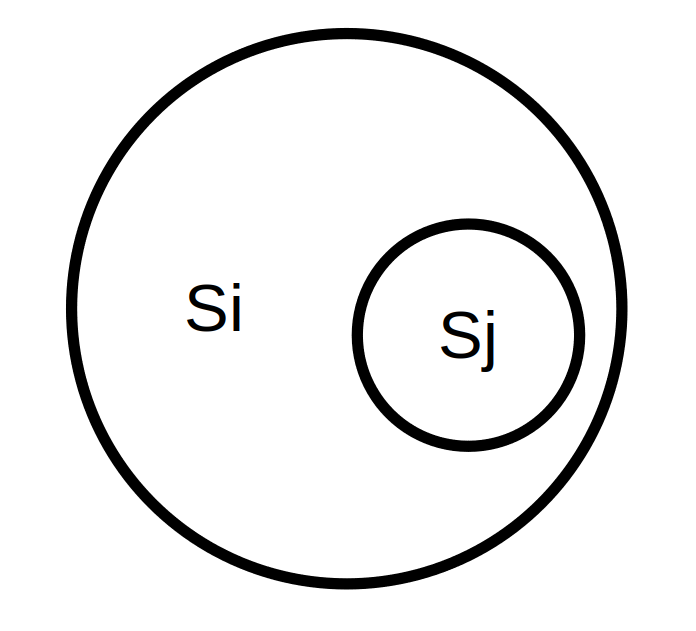
\includegraphics[width=0.4\linewidth]{figures/sd_sets/inclusion2.png}}}

\scnheader{объединение*}
\scnidtf{объединение множеств*}
\scniselement{квазибинарное отношение}
\scniselement{ориентированное отношение}
\scntext{определение}{\textbf{\textit{объединение*}} – это \textit{квазибинарное ориентированное отношение}, областью определения которого является семейство всевозможных множеств. Будем говорить, что \textit{Множество Si} является объединением \textit{Множество Sj} и \textit{Множество Sk} тогда и только тогда, когда любой элемент \textit{Множество Si} является элементом или \textit{Множество Sj} или \textit{Множество Sk}.}
\scnrelfrom{описание типичного экземпляра}{
\scnfilescg {figures/sd_sets/union.png}}
\scnaddlevel{1}
\scnnote{Множество \textit{Si} является объединением множеств \textit{Sj}, \textit{Sk} и \textit{Sm}.}
\scnaddlevel{-1}
\scnrelfrom{изображение}{
\scnfileimage{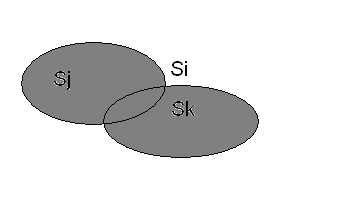
\includegraphics[width=0.6\linewidth]{figures/sd_sets/union2.png}}}

\scnheader{разбиение*}
\scnidtf{разбиение  множества*}
\scnidtf{объединение попарно непересекающихся множеств*}
\scnidtf{декомпозиция множества*}
\scniselement{квазибинарное отношение}
\scniselement{ориентированное отношение}
\scniselement{отношение декомпозиции}
\scntext{определение}{\textbf{\textit{разбиение*}} – это \textit{квазибинарное ориентированное отношение}, областью определения которого является семейство всевозможных множеств. В результате разбиения множества получается множество попарно непересекающихся множеств, объединение которых есть исходное множество.\\
Семейство множеств \{\textit{S1…, Sn}\} является разбиением множества \textit{Si} в том и только том случае, если:
\begin{scnitemize}
    \item семейство \{\textit{S1…, Sn}\} является семейством \textit{попарно непересекающихся множеств};
    \item семейство \{\textit{S1…, Sn}\} является покрытием множества \textit{Si} (или другими словами, множество \textit{Si} является \textit{объединением} множеств, входящих в указанное выше семейство)
\end{scnitemize}
}
\scnrelfrom{описание типичного экземпляра}{
\scnfilescg{figures/sd_sets/split.png}}
\scnaddlevel{1}
\scnnote{Множество \textit{Si} разбивается на множества \textit{Sj}, \textit{Sk} и \textit{Sm}.}
\scnaddlevel{-1}
\scnrelfrom{изображение}{
\scnfileimage{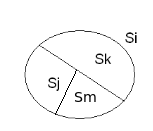
\includegraphics[width=0.5\linewidth]{figures/sd_sets/split2.png}}}

\scnheader{пересечение*}
\scnidtf{пересечение множеств*}
\scniselement{квазибинарное отношение}
\scniselement{ориентированное отношение}
\scntext{определение}{\textbf{\textit{пересечение*}} – это операция над множествами, аргументами которой являются два или большее число множеств, а результатом является множество, элементами которого являются все те и только те сущности, которые одновременно принадлежат каждому множеству, которое входит в семейство аргументов этой операции.\\
Будем говорить, что \textit{Множество Si} является пересечением \textit{Множество Sj} и \textit{Множество Sk} тогда и только тогда, когда любой элемент \textit{Множество Si} является элементом \textit{Множество Sj} и элементом \textit{Множество Sk}.}
\scnrelfrom{описание типичного экземпляра}{
\scnfilescg{figures/sd_sets/intersection.png}}
\scnaddlevel{1}
\scnnote{Множество \textit{Si} является результатом пересечения множеств \textit{Sj}, \textit{Sk} и \textit{Sm}.}
\scnaddlevel{-1}
\scnrelfrom{изображение}{
\scnfileimage{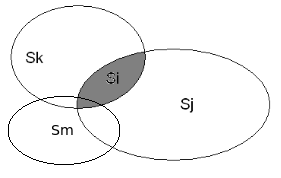
\includegraphics[width=0.5\linewidth]{figures/sd_sets/intersection2.png}}}

\scnheader{пара пересекающихся множеств*}
\scniselement{бинарное отношение}
\scniselement{неориентированное отношение}
\scnexplanation{\textbf{\textit{пара пересекающихся множеств*}} – \textit{бинарное неориентированное отношение} между двумя \textit{множествами}, имеющими непустое \textit{пересечение*}.}
\scntext{определение}{\textbf{\textit{пара пересекающихся множеств*}} – \textit{бинарное неориентированное отношение} между двумя \textit{множествами}, имеющими, по крайней мере, один общий для этих двух множеств элемент.}
\scnrelfrom{описание типичного экземпляра}{
\scnfilescg{figures/sd_sets/pairOfIntersectingSets.png}}
\scnaddlevel{1}
\scnnote{Множество \textit{Si} и множество \textit{Sj} являются парой пересекающихся множеств.}
\scnaddlevel{-1}
\scnrelfrom{изображение}{
\scnfileimage{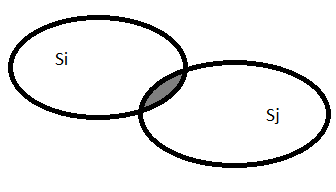
\includegraphics[width=0.5\linewidth]{figures/sd_sets/pairOfIntersectingSets2.png}}}

\scnheader{попарно пересекающиеся множества*}
\scnidtf{семейство попарно пересекающихся множеств*}
\scnsuperset{пересекающиеся множества*}
\scniselement{отношение}
\scntext{определение}{\textbf{\textit{попарно пересекающиеся множества*}} – семейство множеств, каждая пара которых является парой пересекающихся множеств, т.е. каждая пара которых имеет хотя бы один общий элемент}
\scntext{примечание}{Не каждое \textit{семейство попарно пересекающихся множеств*} является \textit{семейством пересекающихся множеств*}, хотя обратное верно.}
\scnrelfrom{изображение}{
\scnfilescg{figures/sd_sets/pairwiseIntersectingSets.png}}
\scnaddlevel{1}
\scnnote{Множества \textit{Si}, \textit{Sj}, \textit{Sk} и \textit{Sl} являются попарно пересекающимися множествами.}
\scnaddlevel{-1}
\scnrelfrom{изображение}{
\scnfileimage{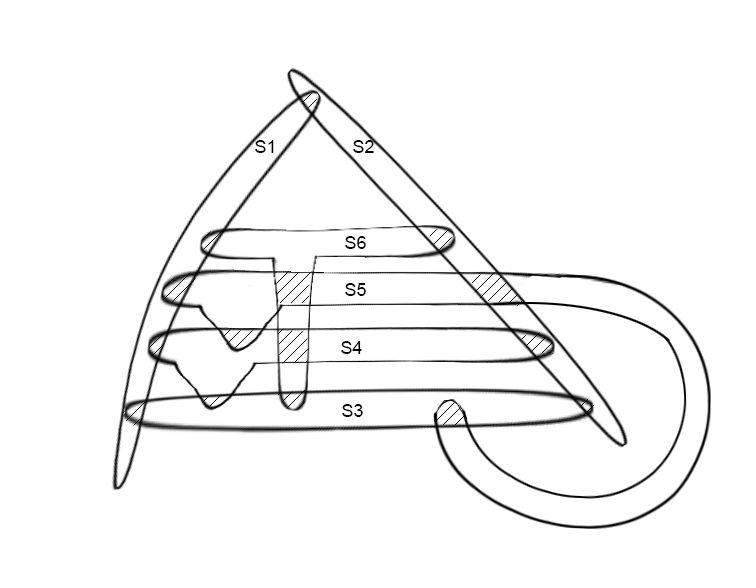
\includegraphics[width=0.7\linewidth]{figures/sd_sets/pairwiseIntersectingSets2.png}}}

\scnheader{пересекающиеся множества*}
\scnidtf{семейство пересекающихся множеств*}
\scnidtf{быть семейством пересекающихся множеств*}
\scnidtf{семейство множеств, имеющих по крайней мере один элемент, являющийся общим для всех этих множеств*}
\scnsuperset{попарно пересекающиеся множества*}
\scntext{определение}{\textbf{\textit{пересекающиеся множества*}} – это семейство множеств, имеющих по крайней мере один общий для всех этих множеств элемент}
\scnrelfrom{описание типичного экземпляра}{
\scnfilescg{figures/sd_sets/intersectingSets.png}}
\scnaddlevel{1}
\scnnote{Множества \textit{Si}, \textit{Sj}, \textit{Sk} и \textit{Sl} являются пересекающимися множествами.}
\scnaddlevel{-1}

\scnheader{пара непересекающихся множеств*}
\scniselement{бинарное отношение}
\scniselement{неориентированное отношение}
\scntext{определение}{\textbf{\textit{пара непересекающихся множеств*}} – это \textit{бинарное неориентированное отношение} между \textit{множествами}, результатом \textit{пересечения*} которых есть пустое множество.}
\scnrelfrom{описание типичного экземпляра}{
\scnfilescg{figures/sd_sets/pairOfNonIntersectingSets.png}}
\scnaddlevel{1}
\scnnote{Множества \textit{Si} и \textit{Sj} являются парой непересекающихся множеств.}
\scnaddlevel{-1}
\scnrelfrom{изображение}{
\scnfileimage{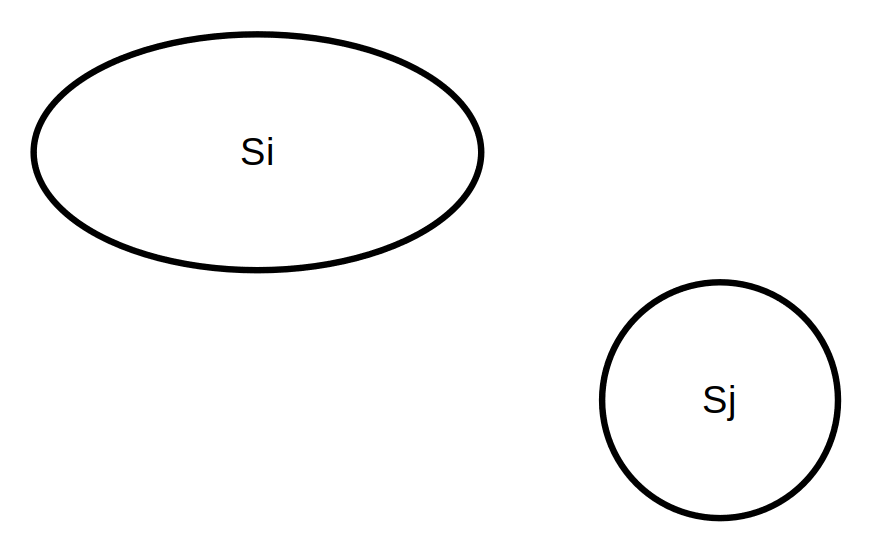
\includegraphics[width=0.5\linewidth]{figures/sd_sets/pairOfNonIntersectingSets2.png}}}

\scnheader{попарно непересекающиеся множества*}
\scnidtf{семейство попарно непересекающихся множеств*}
\scnsubset{непересекающиеся множества*}
\scntext{определение}{\textbf{\textit{попарно непересекающиеся множества*}} – семейство множеств, каждая пара которых является парой непересекающихся множеств, т.е. каждая пара которых не имеет ни одного общего элемента}
\scnrelfrom{изображение}{
\scnfilescg{figures/sd_sets/pairwiseNonIntersectingSets.png}}
\scnaddlevel{1}
\scnnote{Множества \textit{Si}, \textit{Sj}, \textit{Sk} и \textit{Sl} являются попарно непересекающимися множествами.}
\scnaddlevel{-1}

\scnheader{непересекающиеся множества*}
\scnidtf{семейство непересекающихся множеств*}
\scnidtf{быть семейством непересекающихся множеств*}
\scntext{определение}{\textbf{\textit{непересекающиеся множества*}} – это семейство множеств, не имеющих ни одного общего элемента для всех этих множеств}
\scnrelfrom{изображение}{
\scnfilescg{figures/sd_sets/nonIntersectingSets.png}
\scnnote{Множества \textit{Si}, \textit{Sj}, \textit{Sk} и \textit{Sl} являются непересекающимися множествами.}}

\scnheader{разность множеств*}
\scniselement{бинарное отношение}
\scniselement{ориентированное отношение}
\scntext{определение}{\textbf{\textit{разность множеств*}} – это \textit{бинарное ориентированное отношение}, связывающее между собой \textit{ориентированную пару}, первым элементом которой является уменьшаемое множество, вторым - вычитаемое множество, и множество, являющееся результатом вычитания вычитаемого из уменьшаемого, в которое входят все элементы первого множества, не входящие во второе множество.}
\scnrelfrom{описание типичного экземпляра}{
\scnfilescg{figures/sd_sets/setDifference.png}}
\scnaddlevel{1}
\scnnote{Множество \textit{Si} является результатом разности множеств \textit{Sj} и \textit{Sk}.}
\scnaddlevel{-1}
\scnrelfrom{изображение}{
\scnfileimage{
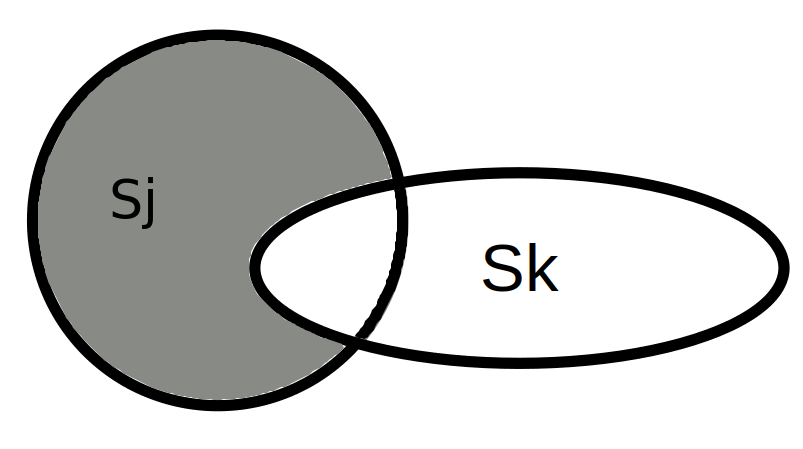
\includegraphics[width=0.5\linewidth]{figures/sd_sets/setDifference2.png}}}

\scnheader{симметрическая разность множеств*}
\scniselement{бинарное отношение}
\scniselement{ориентированное отношение}
\scntext{определение}{\textbf{\textit{симметрическая разность множеств*}} – это \textit{бинарное ориентированное отношение}, связывающее между собой \textit{пару} множеств и множество, являющееся результатом симметрической разности элементов указанной пары. Будем называть \textit{Множество Si} результатом симметрической разности \textit{Множества Sj} и \textit{Множества Sk} тогда и только тогда, когда любой элемент \textit{Множества Si} является или элементом \textit{Множества Sj} или \textit{Множества Sk}, но не является элементом обоих множеств.}
\scnrelfrom{описание типичного экземпляра}{
\scnfilescg{figures/sd_sets/symmetricDifferenceOfSets.png}
\scnnote{Множество \textit{Si} является результатом симметрической разности множеств \textit{Sj} и \textit{Sk}.}}
\scnrelfrom{изображение}{
\scnfileimage{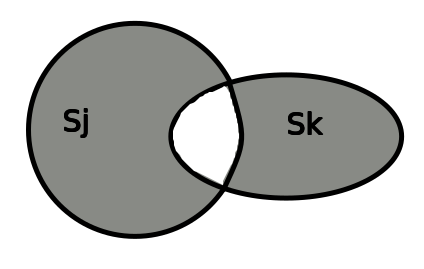
\includegraphics[width=0.5\linewidth]{figures/sd_sets/symmetricDifferenceOfSets2.png}}}

\scnheader{декартово произведение*}
\scnidtf{декартово произведение множеств*}
\scnidtf{прямое произведение множеств*}
\scniselement{бинарное отношение}
\scniselement{ориентированное отношение}
\scntext{определение}{\textbf{\textit{декартово произведение*}} – это \textit{бинарное ориентированное отношение} между \textit{ориентированной парой} множеств и \textit{множеством}, элементами которого являются всевозможные упорядоченные пары, первыми элементами которых являются элементы первого из указанных множеств, вторыми – элементы второго из указанных множеств.}
\scnrelfrom{описание типичного экземпляра}{
\scnfilescg{figures/sd_sets/cartesianMultiplication.png}}
\scnaddlevel{1}
\scnnote{Множество \textit{Si} является результатом декартова произведения множеств \textit{Sj} и \textit{Sk}.}
\scnaddlevel{-1}

\scnheader{декартово произведение}
\scnidtf{второй домен отношения быть декартовым произведением}
\scnrelfrom{второй домен}{декартово произведение*}

\scnheader{семейство подмножеств*}
\scnidtf{семейство подмножеств заданного множества*}
\scniselement{бинарное отношение}
\scniselement{ориентированное отношение}
\scnsuperset{булеан*}
\scntext{определение}{\textbf{\textit{семейство подмножеств*}} – это \textit{бинарное ориентированное отношение} между множеством и некоторым семейством множеств, каждое из которых является подмножеством первого множества.}
\scnrelfrom{описание типичного экземпляра}{
\scnfilescg{figures/sd_sets/familyOfSubsets.png}
}

\scnheader{булеан*}
\scnidtf{булеан множества*}
\scnidtf{семейство всевозможных подмножеств заданного множества*}
\scniselement{бинарное отношение}
\scniselement{ориентированное отношение}
\scntext{определение}{\textbf{\textit{булеан*}} – это \textit{бинарное ориентированное отношение} между множеством и некоторым семейством множеств, каждое из которых является подмножеством первого множества.}
\scnrelfrom{описание типичного экземпляра}{
\scnfilescg{figures/sd_sets/boulean.png}
}

\scnheader{булеан}
\scnidtf{второй домен отношения быть булеаном}
\scnrelfrom{второй домен}{булеан*}

\scnheader{мощность}
\scnidtf{мощность множеств}
\scnidtf{кардинальное число}
\scnidtf{общее число вхождений элементов в заданное множество}
\scnidtf{класс эквивалентности, элементами которого являются знаки всех тех и только тех множеств, которые имеют одинаковую мощность}
\scnidtf{класс эквивалентности, соответствующий отношению быть парой множеств, имеющих одинаковую мощность (равномощность множеств)}
\scnidtf{величина мощности множеств}
\scnidtf{трансфинитное число}
\scnidtf{мощность по Кантору}
\scniselement{параметр}
\scnexplanation{\textbf{\textit{мощность}} – это \textit{параметр}, элементами которых являются \textit{множества}, имеющие одинаковое количество элементов. Значением данного параметра является числовая величина, задающая количество элементов, входящих в данный класс множеств, т.е. по сути, количество \textit{позитивных sc-дуг принадлежности}, выходящих из данного \textit{множества}.

Для двух множеств, имеющих одинаковую мощность, существует взаимно-однозначное соответствие между ними (между множествами вхождений элементов в эти множества – на случай мультимножеств).}
\scnrelfrom{описание типичного экземпляра}{
\scnfilescg{figures/sd_sets/power.png}
}

\scnheader{равенство множеств*}
\scniselement{бинарное отношение}
\scniselement{неориентированное отношение}
\scnidtf{быть равными множествами*}
\scntext{определение}{\textbf{\textit{равенство множеств}}* - бинарное неориентированное отношение, выражающее отношение равенства множеств.

Любые два множества являются равными множествами тогда и только тогда, когда первое является включением второго и второе является включением первого.}
\scnrelfrom{описание типичного экземпляра}{
\scnfilescg{figures/sd_sets/equalityOfSets.png}}
\scnaddlevel{1}
\scnnote{Множество \textit{Si} равно множеству \textit{Sj}.}
\scnaddlevel{-1}

\scnendstruct

\end{SCn}

\scsubsubsection{Предметная область и онтология связок и отношений}
\label{sec:sd_rels}
\begin{SCn}

\scnsectionheader{\currentname}

\scnstartsubstruct

\scnheader{Предметная область связок и отношений}
\scniselement{предметная область}
\scnsdmainclasssingle{связь}
\scnsdclass{бинарная связь;sc-коннектор;неатомарная бинарная связь;небинарная связь;неориентированная связь;ориентированная связь;отношение;класс равномощных связок;класс связок разной мощности;унарное отношение;бинарное отношение;квазибинарное отношение;тернарное отношение;небинарное отношение;ориентированное отношение;неориентированное отношение;рефлексивное отношение;антирефлексивное отношение;частично рефлексивное отношение;симметричное отношение;антисимметричное отношение;частично симметричное отношение;транзитивное отношение;антитранзитивное отношение;частично транзитивное отношение;связанное отношение;отношение порядка;отношение строгого порядка;отношение нестрогого порядка;отношение толерантности;отношение эквивалентности;ролевое отношение;числовой атрибут;неролевое отношение;неролевое бинарное отношение;арность;метаотношение;отношение декомпозиции;отношение интеграции}
\scnsdrelation{область определения*;атрибут отношения*;домен*;первый домен*;второй домен*;композиция отношений*;фактор-множество*;соответствие*;отношение соответствия*;область отправления';область прибытия’;образ';прообраз';всюду определенное соответствие*;частично определенное соответствие*;сюръективное соответствие*;несюръективное соответствие*;однозначное соответствие*;обратное соответствие*;обратимое соответствие*;неоднозначное соответствие*;инъективное соответствие*;взаимно однозначное соответствие*;множество сочетаний*;множество размещений*;множество перестановок*}

\scnheader{связь}
\scnidtf{связка sc-элементов}
\scnidtf{sc-связка}
\scnexplanation{\textbf{\textit{связь}} – множество, являющееся абстрактной моделью связи между описываемыми сущностями, которые или знаки которых являются элементами этого множества.}
\scntext{примечание}{Напомним, что все элементы множества, представленного в SC-коде, являются знаками, но описываемыми сущностями могут быть не только сущности, обозначаемые sc-элементами, но и сами эти sc-элементы.}
\scnsubdividing{бинарная связь;небинарная связь}
\scnsubdividing{неориентированная связь;ориентированная связь}

\scnheader{бинарная связь}
\scnsubdividing{sc-коннектор;неатомарная бинарная связь}
\scntext{примечание}{Данное разбиение осуществляется на основе синтаксического признака, а не семантического, поскольку каждый \textit{sc-коннектор} может быть записан в памяти при помощи семантически эквивалентной конструкции, содержащей знак самой связи и пары принадлежности, ведущие к ее элементам, уточненные, при необходимости ролевыми отношениями.}

\scnheader{sc-коннектор}
\scnidtf{атомарная бинарная связь}
\scnexplanation{Каждый \textbf{\textit{sc-коннектор}} представлен в \textit{sc-памяти} одним \textit{sc-элементом} и семантически эквивалентен конструкции, содержащей знак некоторой \textit{бинарной связи} и пары принадлежности, ведущие к элементам этой связи, уточненные, при необходимости ролевыми отношениями.

Такая конструкция может быть обозначена \textbf{\textit{sc-коннектором}} только в случае, когда роли компонентов соответствующей бинарной связи указываются только при помощи \textit{числовых атрибутов 1’} и \textit{2’} или не уточняются вообще.}

\scnheader{неатомарная бинарная связь}
\scnexplanation{\textbf{\textit{неатомарная бинарная связь}} – \textit{бинарная связь}, роли компонентов которой не могут быть заданы только при помощи \textit{ролевых отношений 1'} и \textit{2'}, или не заданы совсем, а требуют дополнительного уточнения при помощи более частных ролевых отношений.}

\scnheader{небинарная связь}
\scnexplanation{\textbf{\textit{небинарная связь}} – связь, имеющая больше двух элементов.}

\scnheader{неориентированная связь}
\scnsuperset{неориентированное множество}
\scnexplanation{\textbf{\textit{неориентированная связь}} – связь, все элементы которой имеют одинаковые роли (при этом соответствующее ролевое отношение, как правило, явно не указывается).}

\scnheader{ориентированная связь}
\scnsuperset{ориентированное множество}
\scnexplanation{\textbf{\textit{ориентированная связь}} – связь, в которой с помощью ролевых отношений, указываются роли компонентов этой связи.}

\scnheader{отношение}
\scnidtf{класс связей}
\scnidtf{класс sc-связок}
\scnidtf{множество отношений}
\scnidtf{Множество всевозможных отношений}
\scntext{определение}{\textbf{\textit{отношение}}, \textit{заданное на множестве M} – это подмножество \textit{декартового произведения} этого множества самого на себя некоторое количество раз.

В более широком смысле \textbf{\textit{отношение}} – это математическая структура, которая формально определяет свойства различных объектов и их взаимосвязи.}
\scnsubdividing{класс равномощных связок;класс связок разной мощности}
\scnsubdividing{бинарное отношение;небинарное отношение}
\scnsubdividing{ориентированное отношение;неориентированное отношение}
\scnsubdividing{ролевое отношение;неролевое отношение}

\scnheader{класс равномощных связок}
\scnidtf{класс связок фиксированной арности}
\scnidtf{отношение, обладающее свойством арности}
\scnsuperset{унарное отношение}
\scnsuperset{бинарное отношение}
\scnsuperset{тернарное отношение}
\scntext{определение}{\textbf{\textit{класс равномощных связок}} – класс связок, имеющих одинаковую мощность.}

\scnheader{класс связок разной мощности}
\scnidtf{отношение нефиксированной арности}
\scnsubset{небинарное отношение}
\scntext{определение}{\textbf{\textit{класс связок разной мощности}} – класс связок, имеющих разную мощность.}

\scnheader{унарное отношение}
\scnidtf{отношение арности один}
\scnidtf{одноместное отношение}
\scnidtf{множество синглетонов}
\scntext{определение}{\textbf{\textit{унарное отношение}} – это множество таких отношений на множестве M, являющихся любым подмножеством множества M.}

\scnheader{бинарное отношение}
\scnidtf{отношение арности два}
\scnidtf{двухместное отношение}
\scnsuperset{квазибинарное отношение}
\scnsuperset{отношение порядка}
\scnsuperset{отношение толерантности}
\scnsubdividing{рефлексивное отношение;антирефлексивное отношение;частично рефлексивное отношение}
\scnsubdividing{симметричное отношение;антисимметричное отношение;частично симметричное отношение}
\scnsubdividing{транзитивное отношение;антитранзитивное отношение;частично транзитивное отношение}
\scnsubdividing{ролевое отношение;неролевое бинарное отношение}
\scntext{определение}{\textbf{\textit{бинарное отношение}} – это множество таких отношений на множестве \textbf{\textit{M}}, являющихся подмножеством \textit{декартова произведения} множества \textbf{\textit{M}}.\\
Если \textbf{\textit{бинарное отношение R}} задано на \textit{множестве} \textbf{\textit{М}} и два элемента этого множества \textbf{\textit{a}} и \textbf{\textit{b}} связаны данным отношением, то будем обозначать такую связь как \textbf{\textit{aRb}}.}

\scnheader{квазибинарное отношение}
\scnexplanation{\textbf{\textit{квазибинарное отношение}} – множество ориентированных пар, первые компоненты которых являются связками.\\
Таким образом, \textit{sc-дуги}, принадлежащие \textbf{\textit{квазибинарным отношениям}}, всегда выходят из связок.}
\scntext{sc-утверждение}{В область определения квазибинарного отношения будем включать:
\begin{scnitemize}
    \item вторые компоненты ориентированных пар, принадлежащих этому отношению;
    \item элементы первых компонентов ориентированных пар, принадлежащих этому отношению;
    \item других элементов область определения квазибинарного отношения не содержит.
\end{scnitemize}
}

\scnheader{тернарное отношение}
\scnidtf{отношение арности три}
\scnidtf{трехместное отношение}
\scnexplanation{\textbf{\textit{тернарное отношение}} – это множество отношений, связывающих между собой три элемента.}

\scnheader{небинарное отношение}
\scnexplanation{\textbf{\textit{небинарное отношение}} – это множество отношений, хотя бы одна из связок каждого из которых имеет значение мощности больше двух.}

\scnheader{ориентированное отношение}
\scntext{определение}{\textbf{\textit{ориентированное отношение}} – это множество таких отношений, каждая связка которых является ориентированным множеством.}

\scnheader{неориентированное отношение}
\scntext{определение}{\textbf{\textit{неориентированное отношение}} – это множество таких отношений, каждая связка которых является неориентированным множеством.}

\scnheader{рефлексивное отношение}
\scntext{определение}{\textbf{\textit{рефлексивное отношение}} – это \textit{бинарное отношение}, любая пара которого есть канторовское множество.}

\scnheader{антирефлексивное отношение}
\scntext{определение}{\textbf{\textit{антирефлексивное отношение R}} на \textit{множестве} \textbf{\textit{A}} – это \textit{бинарное отношение}, в котором все элементы множества \textbf{\textit{A}} не находятся в отношении \textbf{\textit{R}} к самому себе.}

\scnheader{частично рефлексивное отношение}
\scntext{определение}{\textbf{\textit{частично рефлексивное отношение R}} на \textit{множестве} \textbf{\textit{A}} – это \textit{бинарное отношение},  в котором хотя бы один (но не все) элемент множества \textbf{\textit{A}} находится в отношении \textbf{\textit{R}} к самому себе.}

\scnheader{симметричное отношение}
\scntext{определение}{\textbf{\textit{симметричное отношение R}} на \textit{множестве} \textbf{\textit{A}} – это \textit{бинарное отношение}, в котором для каждой пары элементов \textbf{\textit{а}} и \textbf{\textit{b}} этого множества выполнение отношения \textbf{\textit{aRb}} влечёт выполнение \textbf{\textit{bRa}}.}

\scnheader{антисимметричное отношение}
\scntext{определение}{\textbf{\textit{антисимметричное отношение R}} на \textit{множестве} \textbf{\textit{A}} – это \textit{бинарное отношение}, в котором для каждой пары элементов \textbf{\textit{а}} и \textbf{\textit{b}} этого множества выполнение отношений \textbf{\textit{aRb}} и \textbf{\textit{bRa}} влечёт равенство \textbf{\textit{a}} и \textbf{\textit{b}}.}

\scnheader{частично симметричное отношение}
\scntext{определение}{\textbf{\textit{частично симметричное отношение R}} на \textit{множестве} \textbf{\textit{A}} – это \textit{бинарное отношение}, в котором для каждой пары элементов \textbf{\textit{а}} и \textbf{\textit{b}} (но не для всех таких пар) этого множества выполнение отношения \textbf{\textit{aRb}} влечёт выполнение \textbf{\textit{bRa}}.}

\scnheader{транзитивное отношение}
\scntext{определение}{\textbf{\textit{транзитивное отношение R}} на \textit{множестве} \textbf{\textit{A}} – это \textit{бинарное отношение}, в котором для любых трёх элементов этого множества \textbf{\textit{a, b, c}} выполнение отношений \textbf{\textit{aRb}} и \textbf{\textit{bRc}} влечёт выполнение отношения \textbf{\textit{aRc}}.}

\scnheader{антитранзитивное отношение}
\scntext{определение}{\textbf{\textit{антитранзитивное отношение R}} на \textit{множестве} \textbf{\textit{A}} – это \textit{бинарное отношение}, в котором для любых трёх элементов этого множества \textbf{\textit{a, b, c}} выполнение отношений \textbf{\textit{aRb}} и \textbf{\textit{bRc}} не влечёт выполнение отношения \textbf{\textit{aRc}}.}

\scnheader{частично транзитивное отношение}
\scntext{определение}{\textbf{\textit{частично транзитивное отношение R}} на \textit{множестве} \textbf{\textit{A}} – это \textit{бинарное отношение}, в котором для каждых трёх элементов этого множества \textbf{\textit{a, b, c}} (но не для всех таких троек) выполнение отношений \textbf{\textit{aRb}} и \textbf{\textit{bRc}} влечёт выполнение отношения \textbf{\textit{aRc}}.}

\scnheader{связанное отношение}
\scnsubset{бинарное отношение}
\scntext{определение}{\textbf{\textit{связанное отношение R}} на \textit{множестве} \textbf{\textit{A}} – это \textit{бинарное отношение}, в котором для каждой пары элементов \textbf{\textit{а}} и \textbf{\textit{b}} этого множества выполняется одно из двух отношений: \textbf{\textit{aRb}} или \textbf{\textit{bRa}}.}

\scnheader{отношение порядка}
\scnsubdividing{отношение строгого порядка;отношение нестрогого порядка}
\scntext{определение}{\textbf{\textit{отношение порядка}} – это \textit{бинарное отношение}, обладающее свойством транзитивности и антисимметричности.}

\scnheader{отношение строгого порядка}
\scntext{определение}{\textbf{\textit{отношение строгого порядка}} – это \textit{отношение порядка}, обладающее свойством антирефлексивности.}

\scnheader{отношение нестрогого порядка}
\scntext{определение}{\textbf{\textit{отношение нестрогого порядка}} – это \textit{отношение порядка}, обладающее свойством рефлексивности.}

\scnheader{отношение толерантности}
\scntext{определение}{\textbf{\textit{отношение толерантности}} – это \textit{бинарное отношение}, принадлежащее классам \textit{симметричное отношение} и \textit{рефлексивное отношение}.}

\scnheader{отношение эквивалентности}
\scnidtf{максимальное семейство отношений эквивалентности}
\scnsubset{отношение толерантности}
\scntext{определение}{\textbf{\textit{отношение эквивалентности}} – это \textit{отношение толерантности}, принадлежащее классу \textit{транзитивных отношений}}
\scntext{примечание}{Каждое отношение эквивалентности уточняет то, что мы считаем эквивалентными сущностями, т.е. то, на какие сходства этих сущностей мы обращаем внимание и какие их отличия мы игнорируем (не учитываем).}

\scnheader{ролевое отношение}
\scnidtf{атрибут}
\scnidtf{атрибутивное отношение}
\scnidtf{отношение, которое задает роль элементов в рамках некоторого множества}
\scnidtf{отношение, являющееся подмножеством отношения принадлежности}
\scnrelto{семейство подмножеств}{принадлежность*}
\scnsubset{бинарное отношение}
\scnsuperset{числовой атрибут}
\scnexplanation{\textbf{\textit{ролевое отношение}} – это отношение, являющееся подмножеством отношения принадлежности.}
\scntext{правило идентификации экземпляров}{В конце каждого \textit{идентификатора}, соответствующего экземплярам класса \textbf{\textit{ролевое отношение}}, не являющегося системным, ставится знак «'».

Например:\\
\textit{ключевой экземпляр’}

Из-за ограничений в разрешенном алфавите символов, в системном идентификаторе не может быть использовать знак «'», поэтому в начале каждого \textit{системного идентификатора}, соответствующего экземплярам класса \textbf{\textit{ролевое отношение}} ставится префикс «rrel\_».

Например:\\
\textit{rrel\_key\_sc\_element}}

\scnheader{числовой атрибут}
\scnidtf{порядковый номер}
\scnidtf{номер компонента ориентированной связки}
\scnhaselement{1’; 2’; 3’; 4’; 5’; 6’; 7’; 8’; 9’; 10’}
\scnexplanation{\textbf{\textit{числовой атрибут}} – \textit{ролевое отношение}, задающее порядковый номер элемента некоторой ориентированной связки, не уточняя при этом семантику такой принадлежности. Во многих случаях бывает достаточно использовать числовые атрибуты, чтобы различать компоненты связки, семантика каждого из которых дополнительно оговаривается, например, при определении отношения, которому данная связка принадлежит.}

\scnheader{неролевое отношение}
\scnsubdividing{небинарное отношение;неролевое бинарное отношение}
\scnexplanation{\textbf{\textit{неролевое отношение}} – отношение, не являющееся подмножеством отношения принадлежности.}
\scntext{правило идентификации экземпляров}{В конце каждого \textit{идентификатора}, соответствующего экземплярам класса \textbf{\textit{неролевое отношение}}, не являющегося системным, ставится знак «*».

Например:\\
\textit{включение*}

Из-за ограничений в разрешенном алфавите символов, в системном идентификаторе не может быть использовать знак «*», поэтому в начале каждого \textit{системного идентификатора}, соответствующего экземплярам класса \textbf{\textit{неролевое отношение}} ставится префикс «nrel\_».

Например:\\
\textit{nrel\_inclusion}}

\scnheader{неролевое бинарное отношение}
\scnexplanation{\textbf{\textit{неролевое бинарное отношение}} – \textit{бинарное отношение}, не являющееся \textit{ролевым отношением}.}

\scnheader{арность}
\scnidtf{арность отношения}
\scniselement{параметр}
\scnexplanation{\textbf{\textit{арность}} – это параметр, каждый элемент которого представляет собой класс \textit{отношений}, каждая связка которых имеет одинаковую \textit{мощность}. Значение данного \textit{параметра} совпадает со значением \textit{мощности} каждой из таких связок.}
\scnrelfrom{описание типичного экземпляра}{
\scnfilescg{figures/sd_relations/arity.png}}


\scnheader{область определения*}
\scnidtf{область определения отношения*}
\scniselement{бинарное отношение}
\scnexplanation{\textbf{\textit{область определения*}} – это \textit{бинарное отношение}, связывающее отношение со множеством, являющимся его областью определения.

Областью определения отношения будем называть результат теоретико-множественного объединения всех связок этого отношения, или, другими словами, результат теоретико-множественного объединения всех множеств, являющихся доменами данного отношения.}
\scnrelfrom{описание типичного экземпляра}{
\scnfilescg{figures/sd_relations/domain.png}}

\scnheader{атрибут отношения*}
\scnidtf{ролевой атрибут, используемый в связках заданного отношения*}
\scniselement{бинарное отношение}
\scnexplanation{\textbf{\textit{атрибут отношения*}} – это \textit{бинарное отношение}, связывающее заданное отношение с \textit{ролевым отношением}, используемым в данном отношении для уточнения роли того или иного элемента связок данного отношения.}
\scnrelfrom{описание типичного экземпляра}{
\scnfilescg{figures/sd_relations/relationshipAttribute.png}}


\scnheader{домен*}
\scnidtf{домен отношения по заданному атрибуту*}
\scniselement{бинарное отношение}
\scnexplanation{\textbf{\textit{домен*}} – это \textit{бинарное отношение}, связывающее связку отношения \textit{атрибут отношения*} со множеством, являющимся доменом заданного отношения по заданному атрибуту. Множество \textbf{\textit{di}} является доменом отношения \textbf{\textit{ri}} по атрибуту \textbf{\textit{ai}} в том и только том случае, если элементами этого множества являются все те и только те элементы связок отношения \textbf{\textit{ri}}, которые имеют в рамках этих связок атрибут \textbf{\textit{ai}}.}
\scnrelfrom{описание типичного экземпляра}{
\scnfilescg{figures/sd_relations/domen.png}}


\scnheader{первый домен*}
\scniselement{бинарное отношение}
\scntext{определение}{\textbf{\textit{первый домен*}} – это \textit{бинарное отношение}, связывающее отношение с множеством, являющимся доменом по атрибуту \textbf{\textit {1'}} данного отношения.}
\scnrelfrom{описание типичного экземпляра}{
\scnfilescg{figures/sd_relations/firstDomain.png}}

\scnheader{второй домен*}
\scniselement{бинарное отношение}
\scntext{определение}{\textbf{\textit{второй домен*}} – это \textit{бинарное отношение}, связывающее отношение с множеством, являющимся доменом по атрибуту \textbf{\textit{2'}} данного отношения.}
\scnrelfrom{описание типичного экземпляра}{
\scnfilescg{figures/sd_relations/secondDomain.png}}

\scnheader{композиция отношений*}
\scniselement{квазибинарное отношение}
\scntext{определение}{\textbf{\textit{композиция отношений*}} – это \textit{квазибинарное отношение}, связывающее два бинарных отношения с отношением, являющимся их композицией. Под композицией бинарных отношений \textbf{\textit{R}} и \textbf{\textit{S}} будем понимать множество $\{(x, y) | \exists z(xSz \wedge zRy)\}$}
\scnrelfrom{описание типичного экземпляра}{
\scnfilescg{figures/sd_relations/relationshipComposition.png}}

\scnheader{фактор-множество*}
\scnidtf{быть фактор-множеством*}
\scnidtf{множество всевозможных максимальных множеств из попарно эквивалентных элементов*}
\scnidtf{множество всевозможных классов эквивалентности для заданного отношения эквивалентности*}
\scniselement{бинарное отношение}
\scntext{определение}{\textbf{\textit{фактор множество*}} - это бинарное ориентированное отношение, каждая связка которого связывает некоторое отношение эквивалентности со множеством всех соответствующих этому отношению классов эквивалентности. Каждый такой класс представляет собой максимальное множество сущностей, каждая пара которых принадлежит указанному выше отношению эквивалентности.}
\scnrelfrom{описание типичного экземпляра}{
\scnfilescg{figures/sd_relations/factor_set.png}}

\scnheader{метаотношение}
\scntext{определение}{метаотношение - это \textit{отношение}, в каждой связке которого есть по крайней мере один компонент, являющийся знаком некоторого \textit{отношения}.}

\scnheader{отношение декомпозиции}
\scnhaselement{разбиение*}
\scnhaselement{декомпозиция раздела*}
\scnhaselement{декомпозиция абстрактного объекта*}

\scnheader{отношение интеграции}
\scnhaselement{объединение*}

\scnheader{соответствие*}
\scnidtf{наличие соответствия*}
\scniselement{бинарное отношение}
\scnsubdividing{соответствие между непересекающимися множествами*;соответствие между строго пересекающимися множествами*;соответствие, область отправления и область прибытия которого совпадают*}
\scnsubdividing{всюду определенное соответствие*;частично определенное соответствие*}
\scnsubdividing{сюръекция*;несюръективное соответствие*}
\scnsubdividing{однозначное соответствие*;неоднозначное соответствие*}
\scntext{определение}{\textbf{\textit{соответствие*}} – \textit{бинарное отношение}, заданное на множествах и задающее наличие отношения, в котором участвуют только элементы этих множеств.}
\scnrelfrom{описание типичного экземпляра}{
\scnfilescg{figures/sd_relations/conformity.png}}

\scnheader{отношение соответствия*}
\scniselement{бинарное отношение}
\scntext{определение}{\textbf{\textit{отношение соответствия*}} – \textit{бинарное отношение}, связывающее ориентированную пару множеств, на которых задано \textit{соответствие*} и некоторое подмножество \textit{декартова произведения*} этих \textit{множеств}.}
\scnrelfrom{описание типичного экземпляра}{
\scnfilescg{figures/sd_relations/relationshipConformity.png}}

\scnheader{область отправления'}
\scnidtf{область отправления соответствия’}
\scnidtf{область определения соответствия’}
\scnidtf{первый компонент пары в отношении соответствия’}
\scniselement{ролевое отношение}
\scntext{определение}{\textbf{\textit{область отправления'}} – \textit{ролевое отношение}, указывающее на первый компонент пары в рамках отношения \textit{соответствие*}.}
\scnrelfrom{описание типичного экземпляра}{
\scnfilescg{figures/sd_relations/departureArea.png}}

\scnheader{область прибытия’}
\scnidtf{область прибытия соответствия'}
\scnidtf{область значений соответствия'}
\scniselement{ролевое отношение}
\scntext{определение}{\textbf{\textit{область прибытия’}} – \textit{ролевое отношение}, указывающее на второй компонент пары в рамках отношения \textit{соответствие*}.}
\scnrelfrom{описание типичного экземпляра}{
\scnfilescg{figures/sd_relations/arrivalArea.png}}

\scnheader{образ'}
\scnidtf{образ соответствия’}
\scniselement{ролевое отношение}
\scntext{определение}{\textbf{\textit{образ'}} – \textit{ролевое отношение}, указывающее на второй компонент каждой пары в рамках множества пар, которое является вторым компонентом \textit{отношения соответствия*}.}
\scnrelfrom{описание типичного экземпляра}{
\scnfilescg{figures/sd_relations/form.png}}

\scnheader{прообраз'}
\scnidtf{прообраз соответствия’}
\scniselement{ролевое отношение}
\scntext{определение}{\textbf{\textit{прообраз'}} – \textit{ролевое отношение}, указывающее на первый компонент каждой пары в рамках множества пар, которое является первым компонентом \textit{отношения соответствия*}.}
\scnrelfrom{описание типичного экземпляра}{
\scnfilescg{figures/sd_relations/prototype.png}}

\scnheader{всюду определенное соответствие*}
\scnidtf{полное соответствие*}
\scnidtf{наличие всюду определенного соответствия*}
\scntext{определение}{\textbf{\textit{всюду определенное соответствие*}} – это \textit{соответствие*}, при котором существует \textit{образ’} для каждого элемента \textit{области отправления'} данного \textit{соответствия*}.}
\scnrelfrom{описание типичного экземпляра}{
\scnfilescg{figures/sd_relations/surjection.png}}
\scnrelfrom{изображение}{
\scnfileimage{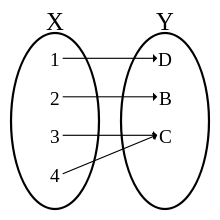
\includegraphics[width=0.5\linewidth]{figures/sd_relations/surjection2.png}}}


\scnheader{частично определенное соответствие*}
\scnidtf{наличие частично определенного соответствия*}
\scntext{определение}{\textbf{\textit{частично определенное соответствие*}} – это \textit{соответствие*}, при котором существует \textit{образ’} для некоторых, но не всех элементов \textit{области отправления'} данного \textit{соответствия*}.}
\scnrelfrom{описание типичного экземпляра}{
\scnfilescg{figures/sd_relations/partiallyDefinedConformity.png}}
\scnrelfrom{изображение}{
\scnfileimage{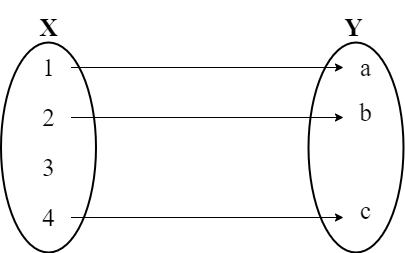
\includegraphics[width=0.5\linewidth]{figures/sd_relations/partiallySurjection.png}}}


\scnheader{сюръективное соответствие*}
\scnidtf{наличие сюръективного соответствия*}
\scnidtf{сюръекция*}
\scntext{определение}{\textbf{\textit{сюръективное соответствие*}} – это \textit{соответствие*}, при котором существует \textit{прообраз’} для каждого элемента \textit{области прибытия'} данного \textit{соответствия*}.}
\scnrelfrom{описание типичного экземпляра}{
\scnfilescg{figures/sd_relations/surjectiveConformity.png}}
\scnrelfrom{изображение}{
\scnfileimage{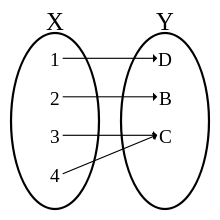
\includegraphics[width=0.5\linewidth]{figures/sd_relations/surjectiveConformity2.png}}}

\scnheader{несюръективное соответствие*}
\scnidtf{наличие несюръективного соответствия*}
\scntext{определение}{\textbf{\textit{несюръективное соответствие*}} – это \textit{соответствие*}, при котором не для каждого элемента \textit{области прибытия'} данного \textit{соответствия*} существует \textit{прообраз’}.}
\scnrelfrom{описание типичного экземпляра}{
\scnfilescg{figures/sd_relations/nonSurjectiveConformity.png}}
\scnrelfrom{изображение}{
\scnfileimage{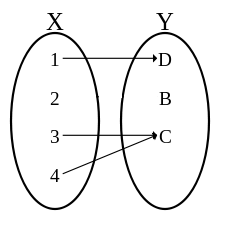
\includegraphics[width=0.5\linewidth]{figures/sd_relations/nonSurjectiveConformity2.png}}}

\scnheader{однозначное соответствие*}
\scnidtf{наличие однозначного соответствия*}
\scnidtf{функциональное соответветствие*}
\scnidtf{функция*}
\scntext{определение}{\textbf{\textit{однозначное соответствие*}} – это \textit{соответствие*}, при котором каждому элементу из \textit{области отправления'} соответствия ставится не более, чем один элемент из \textit{области прибытия’} соответствия.}
\scnrelfrom{описание типичного экземпляра}{
\scnfilescg{figures/sd_relations/singleConformity.png}}
\scnrelfrom{изображение}{
\scnfileimage{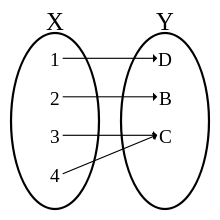
\includegraphics[width=0.5\linewidth]{figures/sd_relations/singleConformity2.png}}}

\scnheader{обратное соответствие*}
\scniselement{бинарное отношение}
\scnrelfrom{область определения}{соответствие*}
\scntext{определение}{\textbf{\textit{обратное соответствие*}} – \textit{бинарное отношение}, связывающее два \textit{соответствия*}, при этом выполняются следующие условия:
\begin{scnitemize}
    \item \textit{область отправления’} первого соответствия является \textit{областью прибытия'} второго;
    \item \textit{область прибытия’} первого соответствия является \textit{областью отправления'} второго;
    \item для каждой пары, входящей в состав отношения первого соответствия, существует пара, входящая в состав отношения второго соответствия, при этом \textit{образ’} и \textit{прообраз'} в рамках первой указанной пары являются соответственно \textit{прообразом'} и \textit{образом’} в рамках второй.
\end{scnitemize}
}

\scnheader{обратимое соответствие*}
\scnsubset{однозначное соответствие*}
\scntext{определение}{\textbf{\textit{обратимое соответствие*}} – такое \textit{однозначное соответствие*}, для которого \textit{обратное соответствие*} также является \textit{однозначным соответствием*}.}

\scnheader{неоднозначное соответствие*}
\scntext{определение}{\textbf{\textit{неоднозначное соответствие*}} – это \textit{соответствие*}, при котором хотя бы одному элементу из \textit{области отправления’} соответствия ставится более, чем один элемент из \textit{области прибытия'} соответствия.}
\scnrelfrom{описание типичного экземпляра}{
\scnfilescg{figures/sd_relations/nonSingleConformity.png}}
\scnrelfrom{изображение}{
\scnfileimage{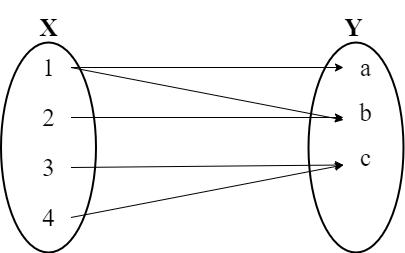
\includegraphics[width=0.5\linewidth]{figures/sd_relations/nonSingleConformity2.png}}}

\scnheader{инъективное соответствие*}
\scnidtf{инъекция*}
\scnsubset{однозначное соответствие*}
\scntext{определение}{\textbf{\textit{инъективное соответствие*}} – это \textit{соответствие*}, при котором разным элементам из \textit{области отправления’} соответствия всегда соответствуют разные элементы из \textit{области прибытия'} соответствия и наоборот.}
\scnrelfrom{описание типичного экземпляра}{
\scnfilescg{figures/sd_relations/injectiveConformity.png}}
\scnrelfrom{изображение}{
\scnfileimage{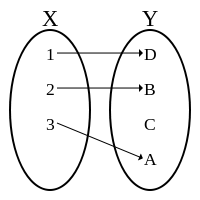
\includegraphics[width=0.5\linewidth]{figures/sd_relations/injectiveConformity2.png}}}

\scnheader{взаимно однозначное соответствие*}
\scnidtf{биекция*}
\scnsubset{всюду определенное соответствие*}
\scnsubset{сюръективное соответствие*}
\scnsubset{инъективное соответствие*}
\scntext{определение}{\textbf{\textit{взаимно однозначное соответствие*}} – это \textit{инъективное соответствие*}, являющееся всюду определенным и сюръективным.}
\scnrelfrom{описание типичного экземпляра}{
\scnfilescg{figures/sd_relations/bijectiveConformity.png}}
\scnrelfrom{изображение}{
\scnfileimage{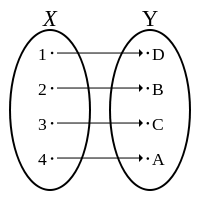
\includegraphics[width=0.5\linewidth]{figures/sd_relations/bijectiveConformity2.png}}}


\scnheader{множество сочетаний*}
\scnidtf{множество всевозможных сочетаний*}
\scnidtf{множество всевозможных сочетаний заданной арности из элементов заданного множества*}
\scnidtf{множество всех неориентированных связок заданной арности*}
\scnidtf{множество всех подмножеств заданной мощности*}
\scnidtf{семейство всевозможных сочетаний*}
\scntext{определение}{\textbf{\textit{множество сочетаний*}} - \textit{отношение}, связывающее некоторое множество и семейство всевозможных множеств, имеющих значение мощности, меньше либо равное мощности исходного множества и состоящих из тех же элементов, что и это множество.}
\scntext{утверждение}{Мощность \textbf{\textit{множества сочетаний*}} может быть вычислена как n!/(k!(n-k)!), где \textbf{\textit{n}} – мощность исходного множества, \textbf{\textit{k}} – мощность элементов множества сочетаний.}
\scnrelfrom{описание типичного экземпляра}{
\scnfilescg{figures/sd_relations/setsOfCombinations.png}
\scntext{комментарий}{Для Множества \textbf{\textit{Si}} представлено множество сочетаний по 2 элемента.}}

\scnheader{множество размещений*}
\scntext{определение}{\textbf{\textit{множество размещений*}} - \textit{отношение}, связывающее некоторое множество и семейство всевозможных кортежей, имеющих значение мощности, меньше либо равное мощности исходного множества и состоящих из тех же элементов, что и это множество.}
\scntext{утверждение}{Мощность \textbf{\textit{множества сочетаний*}} может быть вычислена как n!/(n-k)!, где \textbf{\textit{n}} – мощность исходного множества, \textbf{\textit{k}} – мощность элементов множества сочетаний.}
\scnrelfrom{описание типичного экземпляра}{
\scnfilescg{figures/sd_relations/setsOfPlacements.png}
\scntext{комментарий}{Для Множества \textbf{\textit{Si}} представлено множество размещений по 2 элемента.}}

\scnheader{множество перестановок*}
\scnsubset{множество размещений*}
\scntext{определение}{\textbf{\textit{множество перестановок*}} - \textit{отношение}, связывающее некоторое множество и семейство всевозможных кортежей, равномощных исходному множеству и состоящих из тех же элементов, что и это множество.}
\scntext{утверждение}{Мощность \textbf{\textit{множества перестановок*}} может быть вычислена как n!, где \textbf{\textit{n}} – мощность исходного множества.}
\scnrelfrom{описание типичного экземпляра}{
\scnfilescg{figures/sd_relations/setsOfPermutations.png}
\scntext{комментарий}{Для Множества \textbf{\textit{Si}} представлено его множество перестановок.}}
\scnendstruct

\end{SCn}

\scsubsubsection{Предметная область и онтология свойств, величин и шкал}
\label{sec:sd_params}
\begin{SCn}

\scnsectionheader{Предметная область и онтология параметров, величин и измерений}

\scnstartsubstruct

\scnheader{Предметная область параметров, величин и измерений}
\scnidtf{Предметная область параметров и классов эквивалентности, являющихся их элементами (значениями, величинами)}
\scniselement{предметная область}
\scnsdmainclasssingle{параметр}
\scnsdclass{измеряемый параметр;неизмеряемый параметр;уровень класса эквивалентности;величина;точная величина;неточная величина;интервальная величина;параметрическая модель;измерение с фиксированной единицей измерения ;измерение по шкале;арифметическое выражение на величинах;арифметическая операция на величинах;действие. измерение;задача. измерение}
\scnsdrelation{область определения параметра*;эталон';измерение*;точность*;единица измерения*;нулевая отметка*;единичная отметка*;сумма величин*;произведение величин*;возведение величин в степень*;большая величина*;равенство величин*;большая или равная величина*}

\scnheader{параметр}
\scnidtf{характеристика}
\scnidtf{свойство}
\scnidtf{признак}
\scnidtf{класс классов}
\scnidtf{измеряемое свойство}
\scnidtf{признак классификации или покрытия некоторого класса сущностей}
\scnidtf{признак разбиения или покрытия некоторого класса сущностей}
\scnidtf{семейство множеств, разбивающих или покрывающих некоторый класс сущностей}
\scnidtf{семейство классов сущностей, обладающих одинаковым соответствующим свойством}
\scnidtf{фактор-множество, соответствующее некоторому отношению эквивалентности, или аналог фактор-множества, соответствующий некоторому отношению толерантности}
\scnreltoset{разбиение}{измеряемый параметр;неизмеряемый параметр}
\scnexplanation{Каждый \textbf{\textit{параметр}} представляет собой класс, являющийся семейством всевозможных классов эквивалентности или толерантности, задаваемых либо \textit{отношением эквивалентности}, либо \textit{отношением толерантности} (симметричным, рефлексивным, но частично транзитивным). Так, например, элементами (значениями, величинами) \textbf{\textit{параметра}} \textit{длина} являются либо классы эквивалентности, задаваемые отношением эквивалентности «иметь точно одинаковую длину*», либо классы толерантности, задаваемые отношением вида «иметь приблизительно одинаковую длину с указываемой точностью*», либо интервальные классы, задаваемые бинарными отношениями вида «иметь длину, находящуюся в одном и том же указываемом интервале*» (например, от 1 метра до 2 метров).\\
Примерами параметров как отношений эквивалентности являются:
\begin{scnitemize}
    \item равновеликость геометрических фигур (по длине, площади, объему – в зависимости от размерности этих фигур);
    \item иметь одинаковый цвет (быть эквивалентными по цвету);
    \item эквивалентность, по вкусу, запаху, твердости и т.д.
\end{scnitemize}

Заметим, что среди элементов (значений, величин) параметра могут встречаться пересекающиеся множества (классы), но объединение всех элементов каждого параметра есть не что иное, как класс всевозможных сущностей, обладающих этим параметром (свойством, характеристикой). Например, класс всех сущностей, имеющих длину, класс всех сущностей, обладающих цветом.

Каждый конкретный параметр (характеристика), т.е. каждый элемент класса всевозможных параметров (характеристик) есть, по сути, признак классификации сущностей, обладающих это характеристикой, по принципу эквивалентности (одинаковости значения) этой характеристики. Например, параметр \textit{цвет} разбивает множество сущностей имеющих цвет на классы, каждый из которых включает в себя сущности, имеющие одинаковый цвет. Параметр может разбиваться на классы для уточнения некоторого свойства, например элементами параметра цвет будут классы, соответствующие конкретным цветам (синий, красный и т.д.), в свою очередь каждый конкретный цвет может включать более частные классы, уточняющие данное свойство, например, темно-синий, светло-красный и т.д.

Другими словами, каждому множеству сущностей может ставиться в соответствие набор (семейство) параметров (параметрическое пространство), которыми обладают сущности этого множества – аналог семейства отношений, определенных (заданных) на этом множестве. Часто бывает важно построить такое параметрическое пространство, «точки» которого взаимно-однозначно соответствуют параметризуемым сущностям (например, набор параметров, позволяющих однозначно идентифицировать, установить личность каждого человека). 

Таким образом, для каждого используемого элемента (значения) какого-либо параметра, необходимо явно указывать спецификацию этого значения (точное значение, неточное значение, интервальное значение, точность, интервал).}
\scnrelfrom{типичная семантическая окрестность}{
\scnfilescg{figures/sd_parameters_and_quantities/parameterDescription.png}
}

\scnheader{область определения параметра*}
\scnidtf{множество всех тех и только тех сущностей, которые являются компонентами значений заданного параметра*}
\scnidtf{множество всех тех и только тех сущностей, которые обладают заданным параметром*}
\scnrelto{включение}{объединение*}

\scnheader{измеряемый параметр}
\scnidtf{количественный параметр}
\scnidtf{семейство измеряемых величин}
\scnidtf{семейство классов эквивалентности, каждому из которых может быть поставлено в соответствие числовое значение}
\scnexplanation{Каждый \textbf{\textit{измеряемый параметр}} представляет собой \textit{параметр}, значение (элемент, экземпляр) которого трактуется как \textit{величина}, которой можно поставить в соответствие ее числовое значение на основании выбранной единицы измерения и точки отсчета (нулевой отметки выбранной шкалы).}

\scnheader{неизмеряемый параметр}
\scnidtf{качественный параметр}

\scnheader{уровень класса эквивалентности}
\scnidtf{уровень параметра}
\scniselement{параметр}
\scnexplanation{Параметр \textbf{\textit{уровень класса эквивалентности}} задает уровень некоторого значения некоторого \textit{параметра} в иерархии значений этого параметра. Уровень класса эквивалентности равен 1, если значение параметра не является частным по отношению к другому значению этого параметра, равен 2, если значение параметра является частным по отношению к значению этого параметра с уровнем 1 и т.д.}
\scnrelfrom{типичная семантическая окрестность}{
\scnfilescg{figures/sd_parameters_and_quantities/color.png}
}

\scnheader{величина}
\scnidtf{значение количественного параметра}
\scnidtf{значение измеряемого параметра}
\scnidtf{класс сущностей, имеющих одинаковое значение соответствующего параметра}
\scnrelfromlist{включение}{точная величина;неточная величина;интервальная величина}
\scnexplanation{Каждая \textbf{\textit{величина}} представляет собой однозначный и независящий от шкалы измерения результат измерения некоторой характеристики у некоторой сущности.

Каждой \textbf{\textit{величине}} можно поставить в соответствие ее числовое значение на основании выбранной единицы измерения и точки отсчета (нулевой отметки выбранной шкалы, в случае, если измерение осуществляется по шкале).

Нельзя путать значение параметра (\textbf{\textit{величину}}) и значение величины по некоторой шкале, которое может быть скалярным и векторным.}

\scnheader{точная величина}
\scnidtf{точное значение параметра}
\scnidtf{множество всех точных значений параметра}
\scnidtf{значение параметра, являющееся семейством классов эквивалентности, соответствующим некоторому отношению эквивалентности}
\scnidtf{класс эквивалентности}
\scnexplanation{Каждая \textbf{\textit{точная величина}} имеет одно фиксированное значение в некоторой единице измерения или по какой-либо шкале. При этом считается, что все элементы такого класса имеют одинаковое значение данного параметра и отклонениями можно пренебречь.

Каждой \textbf{\textit{точной величине}} можно поставить в соответствие группу \textit{неточных величин}, являющихся не разбиениями, а покрытиями того же множества, но с разной степенью точности.}
\scnrelfrom{типичная семантическая окрестность}{
\scnfilescg{figures/sd_parameters_and_quantities/exactLength.png}
\scntext{комментарий}{В данном примере \textbf{\textit{ki}} обозначает класс сущностей, имеющих длину ровно 5 метров. Конкретный пример такой сущности - \textbf{\textit{bi}}.}}

\scnheader{неточная величина}
\scnidtf{множество неточных значений параметра}
\scnidtf{приблизительная величина}
\scnidtf{приблизительное значение параметра}
\scnidtf{значение параметра в интервале с нефиксированными границами}
\scnexplanation{Каждой \textbf{\textit{неточной величине}} ставится в соответствие ее значение в некоторой единице измерения или по какой-либо шкале, а также дополнительно указывается \textit{точность*}, т.е. возможное отклонение от данного значения.}
\scnrelfrom{типичная семантическая окрестность}{
\scnfilescg{figures/sd_parameters_and_quantities/approximateLength.png}
\scntext{комментарий}{В данном примере \textbf{\textit{ki}} обозначает класс сущностей, имеющих длину примерно 25 метров, при этом максимально возможное отклонение от этого значения составляет \textbf{\textit{kj}}, то есть 2 метра. Конкретный пример такой сущности - \textbf{\textit{bi}}.}}

\scnheader{интервальная  величина}
\scnidtf{интервальное значение параметра}
\scnidtf{значение параметра в интервале с фиксированными границами}
\scnidtf{интервал значения параметра из множества пересекающихся интервалов разной длины, имеющих нефиксированные границы}
\scnexplanation{Каждая \textbf{\textit{интервальная величина}} представляет собой класс сущностей, находящихся в рамках точно заданного интервала, минимальная и максимальная точка которого являются \textit{точными величинами}. Результатом \textit{измерения*} такой величины является ориентированная пара, первым компонентом которой является левая (меньшая) граница интервала, вторым компонентом – правая (большая) граница интервала.}
\scnrelfrom{типичная семантическая окрестность}{
\scnfilescg{figures/sd_parameters_and_quantities/intervalLength.png}
\scntext{комментарий}{В данном примере \textbf{\textit{ki}} обозначает класс сущностей, имеющих длину, которая лежит в интервале от \textbf{\textit{kj}} до \textit{kl}, то есть в интервале от 4 до 5 метров, а \textbf{\textit{bi}} – конкретный пример такой сущности.}}

\scnheader{эталон'}
\scnidtf{образец'}
\scniselement{ролевое отношение}
\scnexplanation{Ролевое отношение \textit{эталон'} указывает на тот элемент значения некоторого параметра, который в рамках данного класса эквивалентности считается эталонным, то есть он используется как образец при определении данного параметра.

\textit{эталон'} может задаваться как для измеряемых, так и для неизмеряемых параметров, например, эталон метра или эталон красоты.}

\scnheader{измерение*}
\scnidtf{значение параметра*}
\scnidtf{значение величины*}
\scnidtf{измерение как соответствие*}
\scnidtf{результат измерения заданной величины в заданной единице измерения и по заданной шкале*}
\scnidtf{бинарное ориентированное отношение, связывающее различные величины с результатами их измерения в различных единицах измерения и по различным шкалам*}
\scnexplanation{Связки отношения \textit{измерение*} связывают величину и ее значение в некоторой единице измерения (в том числе, в интервале) или по некоторой шкале. Конкретная единица измерения или шкала указывается дополнительно при помощи соответствующего отношения. Одной величине может соответствовать только одно значение в каждой возможной единице измерения или одна точка на некоторой шкале.}

\scnheader{точность*}
\scnidtf{отклонение*}
\scnidtf{степень точности неточного значения параметра*}
\scniselement{бинарное отношение}
\scnexplanation{Связки отношения \textbf{\textit{точность*}} связывают \textit{неточную величину} и \textit{точную величину} того же класса, задающую максимальное возможное отклонение указанной \textit{неточной величины} от своего значения.}

\scnheader{параметрическая модель}
\scnidtf{параметрическая спецификация}
\scnidtf{параметрическое sc-описание заданной сущности}
\scnidtf{описание сущности как точки в некотором параметрическом (признаковом) пространстве}
\scnrelto{включение}{семантическая окрестность}
\scnexplanation{Каждая \textbf{\textit{параметрическая модель}} представляет собой описание заданной сущности в некотором параметрическом пространстве количественных и качественных \textit{параметров}, т.е. указание того, какие значения заданных параметров (характеристик) соответствуют описываемой (заданной) сущности.}

\scnheader{единица измерения*}
\scniselement{бинарное отношение}
\scnexplanation{Связки отношения \textbf{\textit{единица измерения*}} связывают знак конкретного \textbf{\textit{измерения с фиксированной единицей измерения}} и некоторую \textit{точную величину}, входящую в тот же конкретный \textit{параметр}, что и первый компонент связок этого конкретного измерения, и которая используется в данном случае в качестве единицы измерения.}

\scnheader{измерение с фиксированной единицей измерения }
\scnrelto{семейство подмножеств}{измерение*}
\scnexplanation{Каждая \textbf{\textit{измерение с фиксированной единицей измерения}} представляет собой подмножество отношения \textit{измерение*} и характеризуется некоторой \textit{единицей измерения*}, которая является элементом того же параметра (семейством сущностей, имеющих значение данного параметра, совпадающее с этой единицей измерения).}

\scnheader{измерение по шкале }
\scnidtf{шкала}
\scnrelto{семейство подмножеств}{измерение*}
\scnexplanation{Каждая \textbf{\textit{измерение по шкале}} представляет собой подмножество отношения \textit{измерение*} и характеризуется не единицей измерения, а некоторой точкой отсчета для данной \textbf{\textit{шкалы}}. Результатом \textbf{\textit{измерения по шкале}} будет некоторая точка шкалы, отстоящая от точки отсчета на определенное расстояние в нужную сторону (меньшую или большую). Понятно, что это расстояние может быть измерено любыми единицами измерения, но его величина при этом останется неизменной.

Не стоит путать измерение по \textbf{\textit{измерение по шкале}}, которое зависит от \textit{нулевой отметки*}, с измерением изменения того же \textit{параметра}, которое характеризуется единицей измерения и не зависит от точки отсчета. Например, не стоит путать дату по некоторому календарю, соответствующую \textit{началу} какого-либо процесса, и \textit{длительность} этого процесса, которая не зависит от выбранного календаря.}
\scnrelfrom{типичная семантическая окрестность}{
\scnfilescg{figures/sd_parameters_and_quantities/scale.png}
\scntext{комментарий}{В данном примере \textbf{\textit{ki}} обозначает класс сущностей, имеющих точную температуру в 330 К, а \textbf{\textit{bi}} – конкретный пример такой сущности.}}

\scnheader{нулевая отметка*}
\scnidtf{нуль по шкале*}
\scnidtf{начало отсчета*}
\scniselement{бинарное отношение}
\scnexplanation{Связки отношения \textbf{\textit{нулевая отметка*}} связывают знак некоторого \textit{измерения по шкале} со знаком \textit{точной величины} того же \textit{параметра}, которая в рамках данной шкалы принимается за точку отсчета.}

\scnheader{единичная отметка*}
\scnidtf{единица по шкале*}
\scniselement{бинарное отношение}
\scnexplanation{Связки отношения \textbf{\textit{единичная отметка*}} связывают знак некоторого \textit{измерения по шкале} со знаком \textit{точной величины} того же \textit{параметра}, которая в рамках данной шкалы принимается за единичную отметку, т.е. отметку шкалы, отстоящую от нулевой на расстояние, равное выбранной единице измерения. Вместо указания единичной отметки можно использовать указание единицы измерения, однако величина, выбранная в качестве единицы измерения в этом случае будет принадлежать другому измеряемому параметру, характеризующему \uline{изменение} значения величины параметра, измеряемого по шкале.}

\scnheader{арифметическое выражение на величинах}
\scnexplanation{Каждое \textbf{\textit{арифметическое выражение на величинах}} представляет собой \textit{связку}, компонентами которой являются элементы или подмножества некоторого \textit{количественного параметра}.}

\scnheader{арифметическая операция на величинах}
\scnrelto{семейство подмножеств}{арифметическое выражение на величинах}
\scnexplanation{Каждая \textbf{\textit{арифметическая операция на величинах}} представляет собой \textit{отношение}, элементами которого являются \textit{арифметические выражения на величинах}, то есть множество \textit{арифметических выражений на величинах} какого-либо одного вида.}

\scnheader{сумма величин*}
\scnidtf{сложение величин*}
\scniselement{арифметическая операция на величинах}
\scniselement{квазибинарное отношение}
\scnexplanation{\textbf{\textit{сумма величин*}} – это \textit{арифметическая операция на величинах}, аналогичная \textit{арифметической операции сумма*} для \textit{чисел}.

Первым компонентом связки отношения \textbf{\textit{сумма величин*}} является подмножество некоторого \textit{количественного параметра} (слагаемые \textit{величины}), содержащее два или более элемента, вторым компонентом – элемент этого же \textit{количественного параметра}, значение которого в любой \textit{единице измерения*} является результатом сложения значений всех слагаемых \textit{величин} в той же \textit{единице измерения*}. При несовпадении \textit{единиц измерения} слагаемых величин необходимо воспользоваться соотношениями между \textit{единицами измерения}, которые задаются при помощи операций \textit{произведение величин*} и \textit{возведение величин в степень*}.}


\scnheader{произведение величин*}
\scnidtf{умножение величин*}
\scniselement{арифметическая операция на величинах}
\scniselement{квазибинарное отношение}
\scnexplanation{\textbf{\textit{произведение величин*}} – это \textit{арифметическая операция на величинах}, аналогичная \textit{арифметической операции произведение*} для \textit{чисел}.

Первым компонентом связки отношения \textbf{\textit{произведение величин*}} является \textit{связка}, элементами которой являются либо \textit{величины количественных параметров}, либо \textit{числа}, но при этом хотя бы один элемент должен быть \textit{величиной}. Вторым компонентов является \textit{величина количественного параметра}.

Операция \textbf{\textit{произведение величин*}} может быть использована для задания соотношения между \textit{единицами измерения*} в рамках одного \textit{количественного параметра}.}
\scnrelfrom{описание типичного экземпляра}{
\scnfilescg{figures/sd_parameters_and_quantities/multiplicationOfQuantities.png}}

\scnrelfrom{описание типичного экземпляра}{
\scnfilescg{figures/sd_parameters_and_quantities/multiplicationOfQuantities2.png}}

\scnheader{возведение величин в степень*}
\scniselement{арифметическая операция на величинах}
\scniselement{бинарное отношение}
\scnexplanation{\textbf{\textit{возведение величин в степень*}} – это \textit{арифметическая операция на величинах}, аналогичная \textit{арифметической операции возведение в степень*} для \textit{чисел}.

Первым компонентом связки отношения \textbf{\textit{возведение величин в степень*}} является ориентированная пара, первым компонентом которой является \textit{величина количественного параметра} (основание степени), вторым – \textit{число} (показатель степени); Вторым компонентом связки отношения \textbf{\textit{возведение величин в степень*}} является \textit{величина количественного параметра} (результат возведения в степень).}
\scnrelfrom{описание типичного экземпляра}{
\scnfilescg{figures/sd_parameters_and_quantities/exponentiation.png}}

\scnrelfrom{описание типичного экземпляра}{
\scnfilescg{figures/sd_parameters_and_quantities/exponentiationTo2.png}}

\scnheader{большая величина*}
\scniselement{арифметическая операция на величинах}
\scniselement{бинарное отношение}
\scniselement{отношение строгого порядка}
\scnexplanation{\textbf{\textit{большая величина*}} – это \textit{арифметическая операция на величинах}, аналогичная \textit{арифметической операции больше*} для \textit{чисел}.\\
Из двух величин большей является та, \textit{значение} которой в любой \textit{единице измерения*} \textit{больше*} значения другой \textit{величины} в той же \textit{единице измерения}.}

\scnheader{равенство величин*}
\scniselement{арифметическая операция на величинах}
\scniselement{бинарное отношение}
\scniselement{симметричное отношение}
\scniselement{рефлексивное отношение}
\scniselement{транзитивное отношение}
\scnexplanation{\textbf{\textit{равенство величин*}} – это \textit{арифметическая операция на величинах}, аналогичная \textit{арифметической операции равенство*} для \textit{чисел}.

Отношение \textbf{\textit{равенство величин*}} носит исключительно дидактический характер, и явно не указывается, поскольку связывает попарно все элементы одной и той же \textit{величины} каждого \textit{количественного параметра}.}

\scnheader{большая или равная величина*}
\scniselement{арифметическая операция на величинах}
\scniselement{бинарное отношение}
\scniselement{отношение нестрогого порядка}
\scnexplanation{\textbf{\textit{большая или равная величина*}} – это \textit{арифметическая операция на величинах}, аналогичная \textit{арифметической операции больше или равно*} для \textit{чисел}.

В рамках каждой связки данного отношения первая \textit{величина} (первый компонент связки) может быть \textit{большей величиной*} или быть для второй \textit{равной величиной*}.}

\scnheader{действие. измерение}
\scnidtf{измерение как действие}
\scnidtf{действие, направленное на установление связи, принадлежащей отношению измерение* и связывающей величину, которая принадлежит заданному параметру, и которой принадлежит заданная сущность, и соответствующее значение этой величины на некоторой шкале}
\scnidtf{действие, направленное на решение задачи измерения заданного параметра у заданной сущности}
\scnrelto{включение}{действие}

\scnheader{задача. измерение}
\scnidtf{спецификация действия измерения}
\scnidtf{спецификация действия, целью которого является измерение заданного параметра у заданной сущности}
\scnrelto{включение}{задача}

\scnendstruct

\end{SCn}

\scsubsubsection{Предметная область и онтология чисел и числовых структур}
\begin{SCn}

\scnsectionheader{\currentname}

\scnstartsubstruct

\scnheader{Предметная область чисел и числовых структур}
\scniselement{предметная область}
\scnsdmainclasssingle{число}
\scnsdclass{натуральное число;целое число;рациональное число;иррациональное число;действительное число;комплексное число;отрицательное число;положительное число;арифметическое выражение;арифметическая операция;Число Пи;Нуль;Единица;Мнимая единица;числовая структура;система счисления;десятичная система счисления;двоичная система счисления;шестнадцатеричная система счисления; дробь; обыкновенная дробь; десятичная дробь; цифра; арабская цифра; римская цифра}
\scnsdrelation{противоположные числа*;модуль*;сумма*;произведение*;возведение в степень*;больше*;равенство*;больше или равно*}

\scnheader{число}
\scnidtf{множество чисел}
\scnsubset{абстрактная терминальная сущность}
\scnexplanation{\textbf{\textit{число}} -- это основное понятие математики, используемое для количественной характеристики, сравнения, нумерации объектов и их частей. Письменными знаками для обозначения чисел служат \textit{цифры}.}

\scnheader{цифра}
\scnidtf{множество цифр}
\scnsubset{внутренний файл ostis-системы}
\scnrelfromlist{включение}{арабская цифра;римская цифра}
\scnexplanation{\textbf{\textit{цифра}} -– это множество файлов, обозначающих вхождение этой цифры во всевозможные записи чисел с помощью этой цифры.}

\scnheader{натуральное число}
\scnidtf{множество натуральных чисел}
\scnexplanation{\textbf{\textit{натуральное число}} -- это подмножество множества \textit{целых чисел}, которые используются при счете предметов.}
\scnsubset{целое число}

\scnheader{целое число}
\scnidtf{множество целых чисел}
\scnexplanation{\textbf{\textit{целое число}} -- это подмножество множества \textit{рациональных чисел}, получаемых объединением \textit{натуральных чисел} с множеством чисел, \textit{противоположных* натуральным} и \textit{нулём}.}
\scnsubset{рациональное число}

\scnheader{рациональное число}
\scnidtf{множество рациональных чисел}
\scnexplanation{\textbf{\textit{рациональное число}} -- это число, представляемое \textit{обыкновенной дробью}, где числитель — \textit{целое число}, а знаменатель — \textit{натуральное число}.}
\scnsubset{действительное число}

\scnheader{дробь}
\scnidtf{множество дробей}
\scnrelfromlist{включение}{обыкновенная дробь; десятичная дробь}
\scnexplanation{\textbf{\textit{дробь}} — это число, состоящее из одной или нескольких равных частей (долей) единицы}

\scnheader{обыкновення дробь}
\scnidtf{множество обыкновенных дробей}
\scnidtf{множество простых дробей}
\scnexplanation{\textbf{\textit{обыкновенная дробь}} - запись \textit{рационального числа} в виде ${\displaystyle \pm {\frac {m}{n}}}$ или ${\pm m/n}$, где ${n\neq 0}$.Горизонтальная или косая черта обозначает знак деления, в результате которого получается частное. Делимое называется числителем дроби, а делитель — знаменателем.}

\scnheader{десятичная дробь}
\scnidtf{множество десятичных дробей}
\scnexplanation{\textbf{\textit{десятичная дробь}} - Десятичная дробь — разновидность дроби, которая представляет собой способ представления действительных чисел в виде ${\pm d_m \ldots d_1 d_0{,} d_{-1} d_{-2} \ldots}$, где , — десятичная запятая, служащая разделителем между целой и дробной частью числа, ${d_{k}}$m — десятичные цифры.}

\scnheader{иррациональное число}
\scnidtf{множество иррациональных чисел}
\scnexplanation{\textbf{\textit{иррациональное число}} -- это \textit{вещественное число}, которое не является рациональным, то есть не может быть представлено в виде дроби, где числитель — \textit{целое число}, знаменатель — \textit{натуральное число}. Любое \textbf{\textit{иррациональное число}} может быть представлено в виде бесконечной непериодической десятичной дроби.}
\scnsubset{действительное число}

\scnheader{действительное число}
\scnidtf{вещественное число}
\scnidtf{множество вещественных чисел}
\scnreltoset{объединение}{рациональное число;иррациональное число}
\scnsubdividing{положительное число;отрицательное число;$\{$Нуль$\}$}
\scnexplanation{\textbf{\textit{действительное число}} -- это множество чисел, получаемое в результате объединения иррациональных и \textit{рациональных чисел}.}
\scnsubset{комплексное число}

\scnheader{комплексное число}
\scnidtf{множество комплексных чисел}
\scnexplanation{\textbf{\textit{комплексное число}} -- число вида \textit{z=a+b*i}, где \textit{a} и \textit{b} -- \textit{вещественные числа}, \textit{i} -- \textit{Мнимая единица}.}

\scnheader{отрицательное число}
\scnidtf{множество отрицательных чисел}
\scnexplanation{\textbf{\textit{отрицательное число}} -- число \textit{меньше*} нуля.}

\scnheader{положительное число}
\scnidtf{множество положительных чисел}
\scnexplanation{\textbf{\textit{положительное число}} -- число \textit{больше*} нуля.}

\scnheader{противоположные числа*}
\scniselement{бинарное неориентированное отношение}
\scnexplanation{\textbf{\textit{противоположные числа*}} -- \textit{отношение}, связывающее два числа, одно из которых является \textit{отрицательным числом}, второе -- \textit{положительным}, при этом \textit{модули*} этих чисел \textit{равны*}.}

\scnheader{модуль*}
\scnidtf{модуль числа*}
\scniselement{бинарное отношение}
\scnexplanation{Связки отношения \textbf{\textit{модуль*}} связывают некоторое \textit{число} (которое может быть как \textit{отрицательным}, так и \textit{положительным}) и другое \textit{число} (всегда \textit{положительное}), которое выражает расстояние от указанного числа до \textit{Нуля} в единицах.}

\scnheader{арифметическое выражение}
\scnidtf{множество арифметических выражений}
\scnexplanation{Каждое \textbf{\textit{арифметическое выражение}} представляет собой \textit{связку}, компонентами которой являются \textit{числа} или множества \textit{чисел}.}

\scnheader{арифметическая операция}
\scnidtf{множество арифметических операций}
\scnrelto{семейство подмножеств}{арифметическое выражение}
\scnexplanation{Каждая \textbf{\textit{арифметическая операция}} представляет собой \textit{отношение}, элементами которого являются \textit{арифметические выражения}, то есть множество \textit{арифметических выражений} какого-либо одного вида.}

\scnheader{сумма*}
\scnidtf{сложение*}
\scniselement{арифметическая операция}
\scniselement{квазибинарное отношение}
\scnexplanation{\textbf{\textit{сумма*}} -- это арифметическая операция, в результате которой по данным числам (слагаемым) находится новое число (сумма), обозначающее столько единиц, сколько их содержится во всех слагаемых.

Первым компонентом связки отношения \textbf{\textit{сумма*}} является \textit{множество чисел} (слагаемых), содержащее два или более элемента, вторым компонентом -- \textit{число}, являющееся результатом сложения.

Отдельно отметим, что каждая связка отношения \textbf{\textit{сумма*}} вида a = b+c может также трактоваться и как запись о вычитании чисел, например b = a-c, в связи с чем \textit{арифметическая операция} разности чисел отдельно не вводится.}
\scnrelfrom{описание примера}{
\scnfilescg{figures/sd_numbers/sum.png}}

\scnheader{произведение*}
\scnidtf{умножение*}
\scniselement{арифметическая операция}
\scniselement{квазибинарное отношение}
\scnexplanation{\textbf{\textit{произведение*}} -- это \textit{арифметическая операция}, в результате которой один аргумент складывается столько раз, сколько показывает другой, затем результат складывается столько раз, сколько показывает третий и т.д.

Первым компонентом связки отношения \textbf{\textit{произведение*}} является \textit{множество чисел} (множителей), содержащее два или более элемента, вторым компонентом -- \textit{число}, являющееся результатом произведения.

Отдельно отметим, что каждая связка отношения \textbf{\textit{произведение*}} вида a = b*c может также трактоваться и как запись о делении чисел, например b = a/c, в связи с чем \textit{арифметическая операция} деления чисел отдельно не вводится.}
\scnrelfrom{описание примера}{
\scnfilescg{figures/sd_numbers/multiplication.png}}

\scnheader{возведение в степень*}
\scniselement{арифметическая операция}
\scniselement{бинарное отношение}
\scnexplanation{\textbf{\textit{возведение в степень*}} -- это \textit{арифметическая операция}, в результате которой число, называемое основанием степени, умножается само на себя столько раз, каков показатель степени.

Первым компонентом связки отношения \textbf{\textit{возведение в степень*}} является ориентированная пара, первым компонентом которой является \textit{число}, которое является основанием степени, вторым -- \textit{число}, которое является показателем степени; Вторым компонентом связки отношения \textbf{\textit{возведение в степень*}} является \textit{число}, которое является результатом возведения в степень.

Отдельно отметим, что каждая связка отношения \textbf{\textit{возведение в степень*}} вида a = $b^c$ может также трактоваться и как запись об извлечении корня или взятии логарифма, в связи с чем \textit{арифметические операции} извлечения корня и взятия логарифма отдельно не вводится.}
\scnrelfrom{описание примера}{
\scnfilescg{figures/sd_numbers/pow.png}}

\scnheader{больше*}
\scniselement{бинарное отношение}
\scniselement{отношение строгого порядка}
\scnexplanation{\textbf{\textit{больше*}} -- это \textit{бинарное отношение} сравнения чисел. Из двух чисел на координатной прямой больше то, которое расположено правее. Соответственно, первым компонентом связки \textit{отношения} \textbf{\textit{больше*}} является большее из двух \textit{чисел}.}
\scnrelfrom{описание примера}{
\scnfilescg{figures/sd_numbers/more.png}}

\scnheader{больше или равно*}
\scniselement{бинарное отношение}
\scniselement{отношение нестрогого порядка}
\scnexplanation{\textbf{\textit{больше или равно*}} -- это \textit{бинарное отношение} сравнения чисел, при которой первое \textit{число} (первый компонент связки) может быть \textit{больше*} второго или \textit{равняться*} ему.}
\scnnote{Отношение \textit{равенство*} явно не вводится, поскольку в рамках SC-кода равные числа трактуются как совпадающие числа, то есть обозначаемые одним и тем же \textit{sc-элементом}.}
\scnrelfrom{описание примера}{
\scnfilescg{figures/sd_numbers/more_or_equal.png}}

\scnheader{Число Пи}
\scniselement{иррациональное число}
\scnexplanation{\textbf{\textit{Число Пи}} -- это  математическая константа, равная отношению длины окружности к длине её диаметра.}

\scnheader{Нуль}
\scnidtf{0}
\scniselement{целое число}
\scnexplanation{\textbf{\textit{Нуль}} -- это \textit{целое число}, разделяющее на числовой прямой \textit{положительные числа} и \textit{отрицательные числа}.}

\scnheader{Единица}
\scnidtf{1}
\scniselement{целое число}
\scniselement{натуральное число}
\scnexplanation{\textbf{\textit{Единица}} -- это наименьшее \textit{натуральное число}.}

\scnheader{Мнимая единица}
\scnidtf{i}
\scniselement{комплексное число}
\scnexplanation{\textbf{\textit{Мнимая единица}} -- это \textit{число}, при возведении которого в степень 2 результатом будет число, противоположное \textit{Единице}.}

\scnheader{числовая структура}
\scnsubset{структура}
\scnexplanation{\textbf{\textit{числовая структура}} -- \textit{структура}, в состав которой входят знаки \textit{арифметических выражений}, а также знаки их элементов и связи между выражениями и их элементами.}

\scnheader{система счисления}
\scniselement{параметр}
\scnexplanation{Каждая \textbf{\textit{система счисления}} представляет собой класс синтаксически эквивалентных файлов, хранимых в sc-памяти, каждый из которых может являться идентификатором какого-либо \textit{числа}.

Каждая \textbf{\textit{система счисления}} характеризуется алфавитом, т.е. конечным множеством символов (цифр), которые допускается использовать при построении файлов принадлежащих данной \textbf{\textit{системе счисления}}.}

\scnheader{десятичная система счисления}
\scniselement{система счисления}

\scnheader{двоичная система счисления}
\scniselement{система счисления}

\scnheader{шестнадцатеричная система счисления}
\scniselement{система счисления}

\bigskip
\scnendstruct \scnendcurrentsectioncomment

\end{SCn}

\scsubsubsection{Предметная область и онтология структур}
\label{sec:sd_structures}
\begin{SCn}

\scnsectionheader{\currentname}

\scnstartsubstruct

\scnheader{Предметная область структур}
\scnsdmainclasssingle{структура}
\scnsdclass{связная структура;несвязная структура;тривиальная структура;нетривиальная структура;структура второго уровня;семантический уровень структурного элемента;количество семантических уровней элементов структуры}

\scnsdrelation{элемент структуры’;непредставленное множество’;полностью представленное множество’;частично представленное множество’;элемент структуры, не являющийся множеством';максимальное множество’;немаксимальное множество’;первичный элемент’;вторичный элемент’;элемент второго уровня’;метасвязь’;полиморфность*;полиморфизм*;гомоморфность*;гомоморфизм*;изоморфность*;изоморфизм*;автоморфность*;автоморфизм*;аналогичность структур*;сходство*;различие*;первичная синтаксическая структура sc-текста*}

\scnheader{структура}
\scnidtf{sc-структура}
\scnidtf{структура, представленная в виде текста SC-кода}
\scnsubdividing{связная структура;несвязная структура}
\scnsubdividing{тривиальная структура;нетривиальная структура}
\scnexplanation{\textbf{\textit{структура}} — множество \textit{sc-элементов}, удаление одного из которых может привести к нарушению целостности этого множества.}

\scnheader{связная структура}
\scnexplanation{\textit{Структуре}, представленной в \textit{SC-коде}, поставим в соответствие орграф, вершинами которого являются \textit{sc-элементы}, а дугами – пары инцидентности, связывающие \textit{sc-коннекторы} с инцидентными им \textit{sc-элементами}, которые являются компонентами указанных \textit{sc-коннекторов}.

Если полученный таким способом орграф является связным орграфом, то исходную структуру будем считать \textbf{\textit{связной структурой}}.}

\scnheader{несвязная структура}
\scnexplanation{\textit{Структуре}, представленной в \textit{SC-коде}, поставим в соответствие орграф, вершинами которого являются \textit{sc-элементы}, а дугами – пары инцидентности, связывающие \textit{sc-коннекторы} с инцидентными им \textit{sc-элементами}, которые являются компонентами указанных \textit{sc-коннекторов}.

Если полученный таким способом орграф не является связным орграфом, то исходную структуру будем считать \textbf{\textit{несвязной структурой}}.}

\scnheader{тривиальная структура}
\scnidtf{структура первого уровня}
\scnexplanation{\textbf{\textit{тривиальная структура}} – \textit{структура}, не содержащая в качестве элементов связок.}

\scnheader{нетривиальная структура}
\scnsuperset{структура второго уровня}
\scnexplanation{\textbf{\textit{нетривиальная структура}} – \textit{структура}, среди элементов которой есть хотя бы одна связка.}

\scnheader{элемент структуры’}
\scniselement{неосновное понятие}
\scnsubdividing{непредставленное множество';полностью представленное множество’;частично представленное множество’;элемент структуры, не являющийся множеством'}
\scnsubdividing{максимальное множество’;немаксимальное множество'}
\scnexplanation{\textbf{\textit{элемент структуры'}} — \textit{неосновное понятие}, \textit{ролевое отношение}, указывающее на все элементы каждой структуры.

В рамках заданной структуры ее элементы можно классифицировать по заданным признакам:
\begin{scnitemize}
\item насколько полно в рамках \underline{заданной \textit{структуры}} представлено множество, обозначаемое \textit{заданным sc-элементом} вместе с соответствующими дугами принадлежности;
\item существуют ли в рамках \underline{заданной \textit{структуры}} \textit{sc-элементы}, обозначающие множества, являющиеся надмножествами того множества, которое обозначается \underline{заданным \textit{sc-элементом}};
\item уровень («этаж») иерархии перехода от знаков к метазнакам для \underline{заданного \textit{sc-элемента}} в рамках заданной \textit{структуры}.
\end{scnitemize}
}

\scnheader{непредставленное множество’}
\scnidtf{множество, не представленное в рамках данной структуры’}
\scnidtf{быть знаком множества, элементы которого не являются элементами данной структуры'}
\scniselement{ролевое отношение}
\scnexplanation{\textbf{\textit{непредставленное множество’}} – \textit{ролевое отношение}, связывающее структуру со знаком множества, все элементы которого не являются элементами данной структуры.}

\scnheader{полностью представленное множество’}
\scnidtf{множество, полностью представленное в рамках данной структуры'}
\scnidtf{множество, все элементы которого являются элементами данной структуры'}
\scnidtf{полностью представленный класс'}
\scniselement{ролевое отношение}
\scnexplanation{\textbf{\textit{полностью представленное множество’}} – \textit{ролевое отношение}, связывающее \textit{структуру} со знаком множества (любого семантического типа – класса, связки или структуры), все элементы которого являются элементами данной \textit{структуры}.}

\scnheader{частично представленное множество’}
\scnidtf{множество, частично представленное в рамках данной структуры'}
\scnidtf{множество, некоторые элементы которого являются элементами данной структуры'}
\scnidtf{быть знаком множества, некоторые элементы которого являются элементами данной структуры'}
\scniselement{ролевое отношение}
\scnexplanation{\textbf{\textit{частично представленное множество’}} – ролевое отношение, связывающее структуру со знаком множества, не все элементы которого являются элементами данной структуры.}

\scnheader{элемент структуры, не являющийся множеством’}
\scniselement{ролевое отношение}

\scnheader{максимальное множество’}
\scnexplanation{\textbf{\textit{максимальное множество’}} – \textit{ролевое отношение}, связывающее \textit{структуру} со знаком множества, для которого не существует множества, которое было бы надмножеством указанного множества и знак которого был бы элементом этой же структуры.}

\scnheader{немаксимальное множество’}
\scnexplanation{\textbf{\textit{немаксимальное множество’}} – \textit{ролевое отношение}, связывающее \textit{структуру} со знаком множества, для которого в рамках данной \textit{структуры} существует множество, являющееся надмножеством указанного множества.}

\scnheader{первичный элемент’}
\scnidtf{первичный элемент данной структуры'}
\scnidtf{sc-элемент первого уровня в рамках данной структуры'}
\scniselement{ролевое отношение}
\scniselement{семантический уровень структурного элемента}
\scnsubset{элемент структуры’}
\scnexplanation{\textbf{\textit{первичный элемент’}} – ролевое отношение, указывающее на элемент \textit{структуры}, являющийся либо терминальным элементом, либо знаком множества, такого что не существует другого элемента этой же структуры, который был бы элементом множества, обозначаемого первым из указанных элементов структуры. При этом соответствующая пара принадлежности может существовать, но в состав данной структуры не входить.}

\scnheader{вторичный элемент’}
\scnidtf{вторичный элемент данной структуры’}
\scnidtf{элемент данной структуры имеющий семантический уровень более 2'}
\scnidtf{непервичный элемент'}
\scniselement{ролевое отношение}
\scnsubset{элемент структуры’}
\scnexplanation{\textbf{\textit{вторичный элемент’}} – ролевое отношение, указывающее на элемент структуры, обозначающий множество, все или некоторые элементы которого являются элементами указанной структуры.}
\scnsuperset{элемент второго уровня’}

\scnheader{элемент второго уровня’}
\scniselement{ролевое отношение}
\scniselement{семантический уровень структурного элемента}
\scnexplanation{\textbf{\textit{элементом второго уровня’}} в рамках заданной \textit{структуры} может быть связка первичных элементов, тривиальная структура из первичных элементов или класс первичных элементов.}

\scnheader{структура второго уровня’}
\scnexplanation{\textbf{\textit{структура второго уровня}} - \textit{структура}, среди элементов которой есть хотя бы один \textit{элемент второго уровня’}.}

\scnheader{семантический уровень структурного элемента}
\scniselement{параметр}
\scnexplanation{\textbf{\textit{семантический уровень структурного элемента}} представляет собой \textit{параметр}, каждый элемент которого является классом 
\textit{sc-дуг принадлежности}, связывающих некоторую \textit{структуру} с теми ее элементами, который имеют одинаковый семантический уровень в рамках данной структуры. Значением данного параметра является число, обозначающее указанный семантический уровень.

\textbf{\textit{семантический уровень структурного элемента}} вычисляется следующим образом:

\begin{scnitemize}
\item элементы структуры, входящие в нее с атрибутом \textit{первичный элемент'} имеют семантический уровень 1;
\item уровень элемента, не являющегося \textit{первичным элементом'} структуры вычисляется путем прибавления 1 к максимальному из уровней элементов этого элемента (множества), входящих в эту же структуру. Например, \textit{sc-дуга}, соединяющая два \textit{первичных элемента' структуры} будет иметь семантический уровень 2, а \textit{sc-элемент}, обозначающий отношение, которому принадлежит указанная \textit{sc-дуга} – семантический уровень 3.
\end{scnitemize}
}
\scnrelfrom{описание примера}{
\scnfilescg{figures/sd_structures/sem_level_struct_elem.png}
}

\scnheader{количество семантических уровней элементов структуры}
\scniselement{параметр}
\scnexplanation{\textbf{\textit{количество семантических уровней элементов структуры}} – параметр, каждый элемент которого представляет собой класс структур, у которых совпадает максимальный среди семантических уровней элементов этих структур.


Значением данного параметра является число, совпадающее с указанным максимальным семантическим уровнем элементов.}

\scnheader{метасвязь’}
\scniselement{ролевое отношение}
\scnsubset{вторичный элемент’}
\scnexplanation{
\begin{scnenumerate}
    \item Каждая входящая в структуру связь, хотя бы одним компонентом которой является связь, входящая в эту же структуру, элементами которой являются \textit{первичные элементы’} этой структуры, является \textbf{\textit{метасвязью’}} указанной структуры;
    \item Каждая входящая в структуру связь, хотя бы одним компонентом которой является \textbf{\textit{метасвязь’}} этой структуры также является \textbf{\textit{метасвязью’}} указанной структуры;
\end{scnenumerate}
}

\scnheader{полиморфность*}
\scnsubset{соответствие*}
\scniselement{бинарное отношение}
\scnexplanation{\textbf{\textit{полиморфность*}} - это \textit{соответствие}, заданное на \textit{структурах}, при котором каждому элементу из области определения соответствия (первой \textit{структуры}) ставится в соответствие один или более элемент из области значения соответствия (второй \textit{структуры}), при этом существует хотя бы один элемент области определения соответствия, которому соответствуют два или более элемента из области значения соответствия.}

\scnheader{полиморфизм*}
\scniselement{бинарное отношение}

\scnheader{гомоморфность*}
\scnidtf{гомоморфность структур*}
\scnsubset{соответствие*}
\scniselement{бинарное отношение}
\scnexplanation{\textbf{\textit{гомоморфность*}} - это \textit{соответствие}, заданное на \textit{структурах}, при котором каждому элементу из области определения соответствия (первой \textit{структуры}) ставится в соответствие только один элемент из области значения соответствия (второй \textit{структуры}).}
\scnrelfrom{описание примера}{
\scnfilescg{figures/sd_structures/homomorphism.png}
}

\scnheader{гомоморфизм*}
\scniselement{бинарное отношение}

\scnheader{изоморфность*}
\scnidtf{изоморфное соответствие*}
\scnidtf{изоморфность структур*}
\scnsubset{гомоморфность*}
\scniselement{бинарное отношение}
\scnexplanation{\textbf{\textit{изоморфность*}} - это \textit{гомоморфность*}, при которой для каждого элемента из области значения существует ровно один соответствующий элемент из области определения.}
\scnrelfrom{описание примера}{
\scnfilescg{figures/sd_structures/isomorphism.png}
}

\scnheader{изоморфизм*}
\scniselement{бинарное отношение}

\scnheader{автомоморфность*}
\scnsubset{гомоморфность*}
\scniselement{бинарное отношение}
\scnexplanation{\textbf{\textit{автоморфность*}} - это \textit{изоморфность*}, у которой область определения соответствия и область значения соответствия совпадают.}
\scnrelfrom{описание примера}{
\scnfilescg{figures/sd_structures/automorphism.png}}

\scnheader{автоморфизм*}
\scniselement{бинарное отношение}

\scnheader{аналогичность структур*}
\scnsubset{соответствие*}
\scniselement{бинарное отношение}
\scnexplanation{\textbf{\textit{аналогичность структур*}} - \textit{соответствие*}, задаваемое на структурах, и фиксирующее факт наличия некоторой аналогии на подструктурах (подмножествах) указанных структур. Каждой ориентированной паре, принадлежащей \textbf{\textit{аналогичности структур*}} может быть поставлено в соответствие множество пар, задающих \textit{сходства*} некоторых подструктур и \textit{различия*} некоторых подструктур исходных структур.}
\scnrelfrom{описание примера}{
\scnfilescg{figures/sd_structures/analogy.png}}

\scnheader{сходство*}
\scniselement{бинарное отношение}

\scnheader{различие*}
\scniselement{бинарное отношение}

\scnheader{первичная синтаксическая структура sc-текста*}
\scniselement{бинарное отношение}
\scnexplanation{\textbf{\textit{первичная синтаксическая структура sc-текста*}} - это бинарное отношение, связывающее некоторый \textit{sc-текст} с другим \textit{sc-текстом}, формируемым по следующим правилам:
\begin{scnitemize}
    \item каждому \textit{sc-узлу} первого \textit{sc-текста} соответствует \textit{синглетон} (\textit{знак sc-узла}) в рамках второго \textit{sc-текста};
    \item каждому \textit{sc-коннектору} из первого \textit{sc-текста} в рамках второго \textit{sc-текста} соответствует \textit{синглетон}, обозначающий данный \textit{sc-коннектор} и соединенный с другими \textit{синглетонами} второго \textit{sc-текста} парами инцидентности двух типов, в зависимости от того, началом или концом данного \textit{sc-коннектора} являются обозначаемые этими \textit{синглетонами sc-элементы}. В случае, когда \textit{sc-коннектор} является \textit{sc-ребром}, то достаточно пар инцидентности первого типа.
    \item для каждого \textit{синглетона} в рамках второго \textit{sc-текста} явно указывается синтаксический тип, определяемый типом соответствующего ему элемента из первого \textit{sc-текста} (\textit{знак sc-константы}, \textit{знак sc-узла} и т.п.).
\end{scnitemize}


Стоит отметить, что подобным образом может быть задана синтаксическая структура любого текста, а не только sc-текста. В этом случае понадобятся другие отношения инцидентности другие классы синтаксических типов.}
\scnrelfrom{описание примера}{
\scnfilescg{figures/sd_structures/primary_sc_syntax.png}}

\scnendstruct \scnendcurrentsectioncomment

\end{SCn}

\scsubsubsection{Предметная область и онтология теоретико-множественных онтологий}
\scsubsubsection{Предметная область и онтология материальных сущностей}
\scsubsubsection{Предметная область и онтология персон}
\scsubsubsection{Предметная область и онтология пространственных сущностей и их форм}
\scsubsubsection{Предметная область и онтология темпоральных сущностей}
\label{sec:sd_temp_entities}
\begin{SCn}

\scnsectionheader{\currentname}

\scnstartsubstruct

\scnheader{Предметная область темпоральных сущностей}
\scnidtf{Предметная область темпоральных связей и отношений}
\scnidtf{Предметная область временных сущностей}
\scniselement{предметная область}
\scnsdmainclasssingle{временная сущность}
\scnsdclass{прошлая сущность;настоящая сущность;будущая сущность;временная связь;ситуация;процесс;процесс в sc-памяти;процесс во внешней среде ostis-системы;материальная сущность;воздействие;отношение;класс временных связей;класс временных и постоянных связей;множество;ситуативное множество;неситуативное множество;частично ситуативное множество;темпоральная связь;темпоральное отношение;начало;завершение;длительность;тысячелетие;век;год;месяц;сутки;час;минута;секунда}
\scnsdrelation{воздействующая сущность*;объект воздействия*;начальная ситуация*;причинная ситуация*;конечная ситуация*;событие*;последний добавленный sc-элемент\scnrolesign;темпоральное включение*;темпоральная часть*;начальный этап*;конечный этап*;промежуточный этап*;темпоральное включение без совпадения начальных и конечных моментов*;темпоральное включение с совпадением начальных моментов*;темпоральное включение с совпадением конечных моментов*;темпоральное совпадение*;темпоральное объединение*;темпоральная декомпозиция*;темпоральная смежность*;темпоральная последовательность с промежутком*;темпоральная последовательность с пересечением*;номер тысячелетия\scnrolesign;номер века\scnrolesign;номер года\scnrolesign;номер месяца в году\scnrolesign;номер суток в месяце\scnrolesign;номер часа в дне\scnrolesign;номер минуты в часе\scnrolesign;номер секунды в минуте\scnrolesign}

\scnheader{временная сущность}
\scnidtf{временно существующая сущность}
\scnidtf{нестационарная сущность}
\scnidtf{сущность, имеющая и/или начало, и/или конец своего существования}
\scnidtf{sc-элемент, являющийся знаком некоторой временно существующей сущности}
\scnidtf{сущность, обладающая темпоральными характеристиками (длительностью, начальным моментом, конечным моментом и т.д.)}
\scnsubdividing{прошлая сущность;настоящая сущность;будущая сущность}
\scnsubdividing{временная связь;ситуация;процесс;материальная сущность}
\scnexplanation{Следует отличать:
\begin{scnitemize}
    \item временный характер сущности, обозначаемой \textit{sc-элементом};
    \item временный характер существования самого \textit{sc-элемента} в рамках \textit{sc-памяти};
\end{scnitemize}
В ходе обработки информации каждый \textit{sc-элемент} может быть удален из \textit{sc-памяти}.}

\scnheader{прошлая сущность}
\scnidtf{сущность, существовавшая в прошлом времени}
\scnidtf{сущность прошлого времени}
\scnidtf{сущность, завершившая свое существование}

\scnheader{настоящая сущность}
\scnidtf{сущность, существующая в текущий момент времени}
\scnidtf{сущность, существующая сейчас}
\scnidtf{сущность настоящего времени}

\scnheader{будущая сущность}
\scnidtf{возможно будущая сущность}
\scnidtf{прогнозируемая временная сущность}
\scnidtf{временная сущность, которая может существовать в будущем}
\scnidtf{сущность, которая может или должна начать свое существование в будущем времени}
\scnrelfrom{включение}{инициированное действие}
\scnexplanation{Каждой \textbf{\textit{будущей сущности}} можно поставить в соответствие вероятность ее возникновения.}

\scnheader{временная связь}
\scnidtf{нестационарная связь}
\scnidtf{временно существующая связь}
\scnexplanation{Каждая \textbf{\textit{временная связь}} представляет собой \textit{связку}, принадлежащую множеству \textit{временных сущностей}.

Понятие \textbf{\textit{временной связи}} не следует путать с понятием \textit{темпоральной связи}, которая сама является \textit{постоянной сущностью}, описывающей то, как связаны во времени некоторые \textit{временные сущности}.
}

\scnheader{ситуация}
\scnidtf{состояние}
\scnidtf{временная структура}
\scnidtf{временно существующая структура}
\scnidtf{квазистационарная структура}
\scnidtf{состояние некоторой динамической системы, описываемое с некоторой степенью детализации (подробности)}
\scnidtf{квазистационарная структура, существующая временно (в течение некоторого отрезка времени)}
\scnrelto{включение}{структура}
\scnexplanation{Под ситуацией понимается \textit{структура}, содержащая, по крайней мере, один элемент, который является \textit{временной сущностью}. Наличие в рамках ситуации нескольких \textit{временных сущностей} говорит о том, что существует момент времени (в прошлом, настоящем или будущем), в который все они существуют одновременно.}

\scnheader{процесс}
\scnidtf{процесс преобразования некоторой временной сущности из одного состояния в другое}
\scnidtf{процесс перехода от одной ситуации к другой}
\scnidtf{переходный процесс}
\scnidtf{абстрактный процесс}
\scnidtf{информационная модель некоторых преобразований}
\scnidtf{динамическая sc-модель}
\scnidtf{динамическая структура}
\scnrelfrom{включение}{воздействие}
\scnrelto{включение}{структура}
\scnexplanation{Каждый \textbf{\textit{процесс}} определяется (задается) либо возникновением или исчезновением связей, связывающих заданную \textit{временную сущность} с другими сущностями, либо возникновением или исчезновением связей, связывающих части указанной \textit{временной сущности} с другими сущностями. 

Многим \textbf{\textit{процессам}} можно поставить в соответствие \textit{ситуацию}, которая является его \textit{начальной ситуацией*} и \textit{ситуацию}, которая является его \textit{конечной ситуацией*}, то есть указать \textit{ситуации}, переход между которыми осуществляется в ходе \textbf{\textit{процесса}}.

При этом знаки тех \textit{временных сущностей}, с которыми связаны изменения, описываемые некоторым \textbf{\textit{процессом}}, входят в данный \textbf{\textit{процесс}} как элементы и при необходимости уточняются дополнительными \textit{ролевыми отношениями}.}
\scnsubdividing{процесс в sc-памяти;процесс во внешней среде ostis-системы}

\scnheader{процесс в sc-памяти}

\scnheader{процесс во внешней среде ostis-системы}

\scnheader{материальная сущность}
\scnexplanation{Каждой \textbf{\textit{материальной сущности}} можно поставить в соответствие различные \textit{процессы}, описывающие ее преобразование из одного состояния в другое.}

\scnheader{воздействие}
\scnidtf{процесс, осуществляющийся на основе (в результате) воздействия одной сущности на другую}
\scnrelfrom{включение}{действие}
\scnexplanation{Каждому \textbf{\textit{воздействию}} может быть поставлена в соответствие (1) некоторая \textit{воздействующая сущность*}, т.е. сущность, осуществляющая \textbf{\textit{воздействие}} (в частности, это может быть некоторое физическое поле), и (2) некоторый \textit{объект воздействия*}, т.е. сущность, на которую воздействие направлено. Если \textbf{\textit{воздействие}} связано с \textit{материальной сущностью}, то его объектом воздействия является либо сама эта \textit{материальная сущность}, либо некоторая ее пространственная часть.}

\scnheader{воздействующая сущность*}

\scnheader{объект воздействия*}

\scnheader{исходная ситуация*}
\scnidtf{начальная ситуация процесса*}
\scnidtf{начальная ситуация*}
\scniselement{бинарное отношение}
\scnexplanation{Связки отношения \textbf{\textit{исходная ситуация*}} связывают некоторый \textit{процесс} и некоторую ситуацию, являющуюся начальной для этого \textit{процесса}, и, как правило, изменяемой в течение выполнения этого \textit{процесса}.

Первым компонентом каждой связки отношения \textbf{\textit{исходная ситуация*}} является знак \textit{процесса}, вторым – знак начальной \textit{ситуации}.}

\scnheader{причинная ситуация*}
\scniselement{бинарное отношение}
\scnrelto{включение}{начальная ситуация*}
\scnexplanation{Под причинной ситуацией понимается такая \textit{начальная ситуация*}, которая обладает достаточной полнотой для однозначного задания инициируемого \textit{процесса}.}

\scnheader{конечная ситуация*}
\scnidtf{конечная ситуация процесса*}
\scnidtf{результирующая ситуация*}
\scniselement{бинарное отношение}
\scnexplanation{Связки отношения \textbf{\textit{конечная ситуация*}} связывают некоторый \textit{процесс} и некоторую \textit{ситуацию}, ставшую результатом выполнения этого \textit{процесса}, то есть его следствием.

Первым компонентом каждой связки отношения \textbf{\textit{конечная ситуация*}} является знак \textit{процесса}, вторым – знак конечной \textit{ситуации}.}

\scnheader{событие*}
\scniselement{бинарное отношение}
\scnexplanation{Связки отношения \textbf{\textit{событие*}} связывают знак процесса и ориентированную пару, первым компонентом которой является знак \textit{начальной ситуации*} данного процесса, вторым компонентом – знак \textit{конечной ситуации*} данного процесса.}
\scnrelfrom{типичная семантическая окрестность}{
\scnfilescg{figures/sd_temp_entities/event.png}
}

\scnheader{отношение}
\scnsubdividing{класс временных связей;класс постоянных связей;класс временных и постоянных связей}

\scnheader{класс временных связей}
\scnidtf{отношение, все связки которого являются нестационарными}
\scnexplanation{В общем случае \textbf{\textit{класс временных связей}} не является \textit{ситуативным множеством}, поскольку факт принадлежности некоторой \textit{временной связи} такому классу следует считать постоянным, а не временным, поскольку временность/постоянство связи и ее семантический тип, задаваемый классом (отношением), это принципиально разные параметры (характеристики, признаки) любой связи.}

\scnheader{класс постоянных связей}
\scnidtf{отношение, все связки которого являются стационарными}

\scnheader{класс временных и постоянных связей}
\scnidtf{отношение, некоторые (но не все) связки которого являются нестационарными}

\scnheader{множество}
\scnsubdividing{ситуативное множество;неситуативное множество;частично ситуативное множество}

\scnheader{ситуативное множество}
\scnidtf{полностью ситуативное множество}
\scnexplanation{Под \textbf{\textit{ситуативным множеством}} понимается постоянное множество, у которого все выходящие из него связи принадлежности являются \textit{временными сущностями}.

В частности, ситуативное множество может использоваться как вспомогательная динамическая структура, которая содержит элементы некоторых структур, обрабатываемые в данный момент, например, это может быть копия некоторого множества, из которой постепенно удаляются элементы по мере их просмотра и обработки. В случае, когда такая структура содержит всего один элемент, ее можно считать \underline{указателем} на данный элемент, при этом в разные моменты времени это могут быть разные элементы.}

\scnheader{последний добавленный sc-элемент’}
\scniselement{ролевое отношение}

\scnheader{неситуативное множество}
\scnexplanation{Под \textbf{\textit{неситуативным множеством}} понимается постоянное множество, у которого все выходящие из него связи принадлежности являются \textit{постоянными сущностями}.}

\scnheader{частично ситуативное множество}
\scnexplanation{Под \textbf{\textit{частично ситуативным множеством}} понимается постоянное множество, у которого некоторые (но не все) выходящие из него связи принадлежности являются \textit{временными сущностями}.}

\scnheader{темпоральная связь}
\scnidtf{постоянная связь, описывающая связь во времени между временными сущностями}

\scnheader{темпоральное отношение}
\scnrelto{семейство подмножеств}{темпоральная связь}
\scnidtf{класс темпоральных связей}
\scnidtf{отношение, задающее темпоральные связи между временными сущностями}
\scnhaselement{темпоральное включение*}
\scnhaselement{темпоральное объединение*}
\scnhaselement{темпоральная декомпозиция*}
\scnhaselement{темпоральная смежность*}
\scnhaselement{темпоральная последовательность с промежутком*}
\scnhaselement{темпоральная последовательность с пересечением*}

\scnheader{темпоральное включение*}
\scnexplanation{Связки отношения \textbf{\textit{темпоральное включение*}} связывают две \textit{временные сущности}, период существования одной из которых полностью включается в период существования второй.\\
Первым компонентом каждой связки отношения \textbf{\textit{темпоральное включение*}} является знак \textit{временной сущности}, \textit{длительность} существования которой больше.}
\scnrelfromlist{включение}{темпоральная часть*;темпоральное включение без совпадения начальных и конечных моментов*;темпоральное совпадение*;темпоральное включение с совпадением начальных моментов*;темпоральное включение с совпадением конечных моментов*}

\scnheader{темпоральная часть*}
\scnidtf{этап (период) заданной временной сущности*}
\scnidtf{этап процесса существования временной сущности*}
\scnrelfromlist{включение}{начальный этап*;конечный этап*;промежуточный этап*}
\scnrelfrom{типичная семантическая окрестность}{
\scnfilescg{figures/sd_temp_entities/temporal_part.png}
}
\scnrelfrom{иллюстрация}{
\scnfileimage{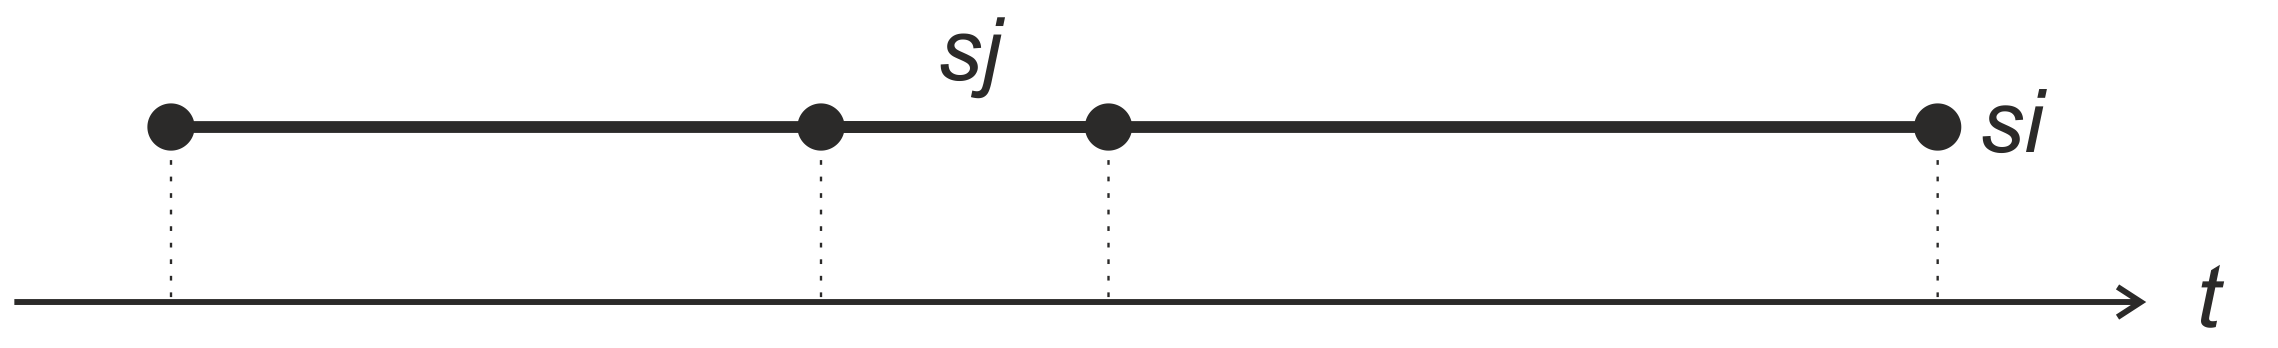
\includegraphics[width=1\linewidth]{figures/sd_temp_entities/img_temporal_part.png}}}
\scntext{примечание}{Связки отношения \textbf{\textit{темпоральная часть*}} связывают две \textit{временные сущности}, одна из которых является частью другой, например, действие и одно из его поддействий. Соответственно, период существования одной из этих сущностей всегда будет включаться в период существования другой (большей).

В отличие от более общего отношения \textit{темпоральное включение*}, связки которого могут связывать любые \textit{временные сущности}, связки отношения \textbf{\textit{темпоральное включение*}} связывают только \textit{временные сущности}, одна из которых является частью другой.}

\scnheader{начальный этап*}

\scnheader{конечный этап*}

\scnheader{промежуточный этап*}

\scnheader{темпоральное включение без совпадения начальных и конечных моментов*}
\scnidtf{строгое темпоральное включение*}
\scnrelfrom{типичная семантическая окрестность}{
\scnfilescg{figures/sd_temp_entities/strict_temporal_inclusion.png}}
\scnrelfrom{иллюстрация}{
\scnfileimage{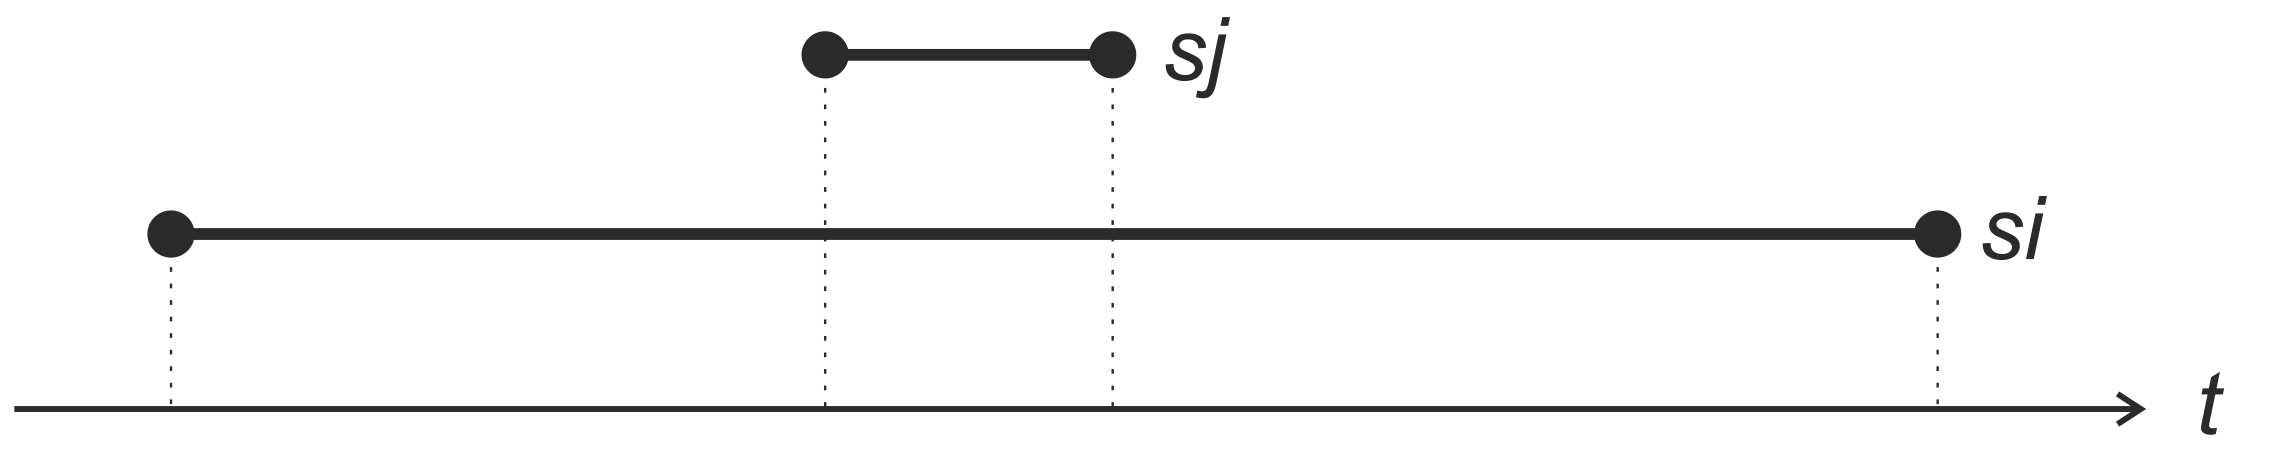
\includegraphics[width=1\linewidth]{figures/sd_temp_entities/img_strict_temporal_inclusion.png}}}
%
% темпоральное включение без совпадения начальных и конечных %моментов
%

\scnheader{темпоральное включение с совпадением начальных моментов*}
\scnrelfrom{типичная семантическая окрестность}{
\scnfilescg{figures/sd_temp_entities/temporal_include_with_match_start_points.png}}
\scnrelfrom{иллюстрация}{
\scnfileimage{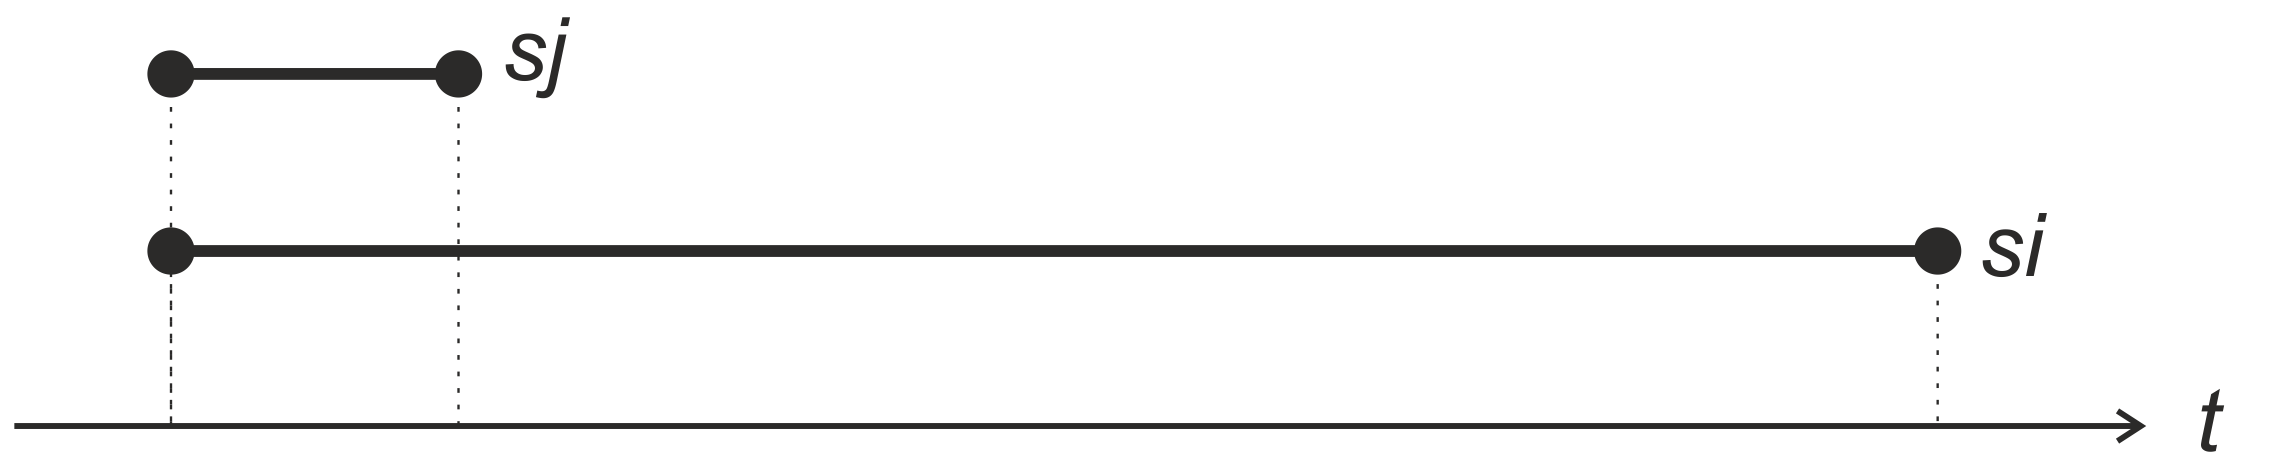
\includegraphics[width=1\linewidth]{figures/sd_temp_entities/img_temporal_include_with_match_start_points.png}}}

\scnheader{темпоральное включение с совпадением конечных моментов*}
\scnrelfrom{типичная семантическая окрестность}{
\scnfilescg{figures/sd_temp_entities/temporal_include_with_terminal_point_match.png}}
\scnrelfrom{иллюстрация}{
\scnfileimage{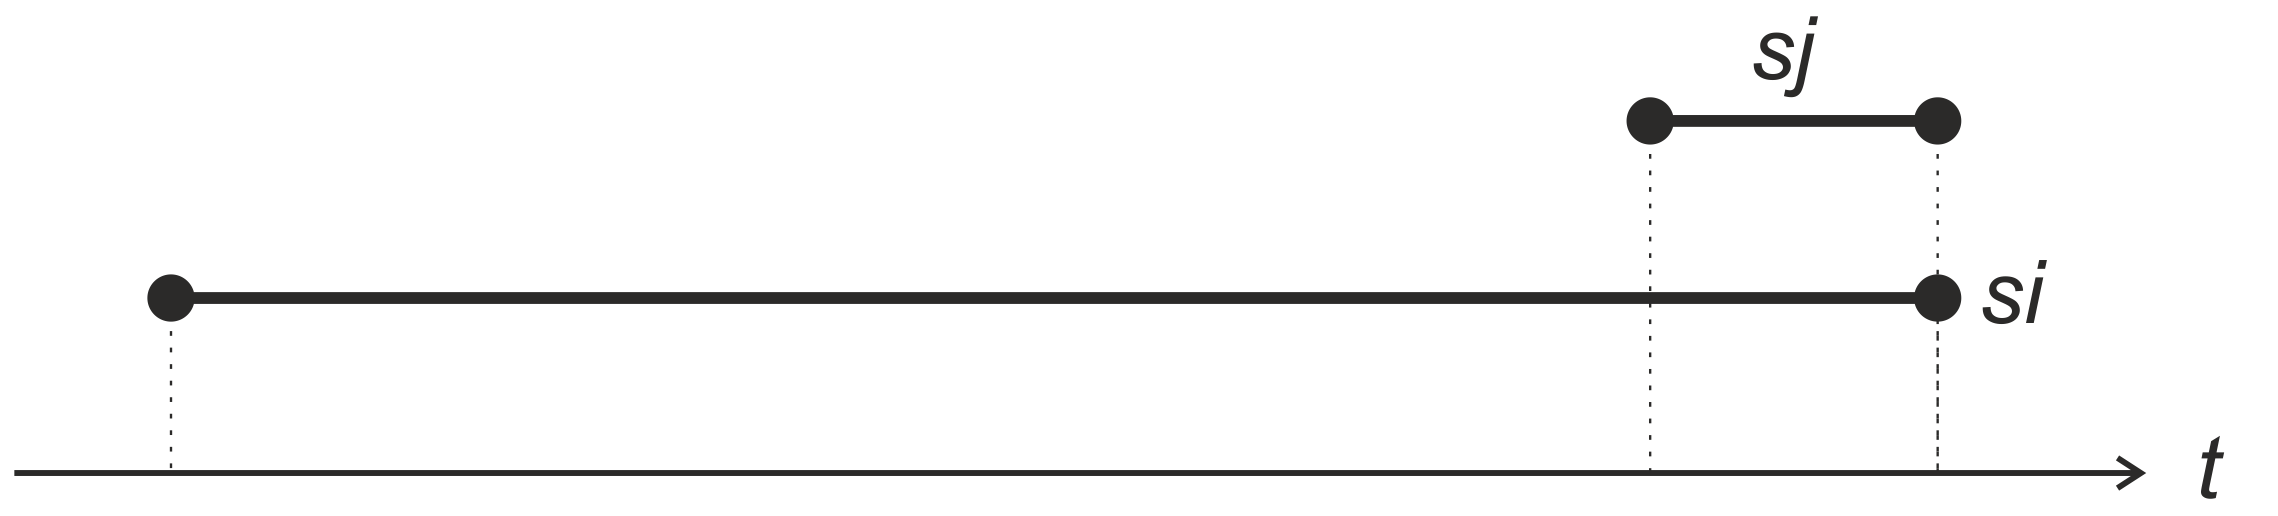
\includegraphics[width=1\linewidth]{figures/sd_temp_entities/img_temporal_include_with_terminal_point_match.png}}}

\scnheader{темпоральное совпадение*}
\scnidtf{совпадение начала и завершения*}

\scnheader{темпоральное объединение*}
\scnrelfrom{типичная семантическая окрестность}{
\scnfilescg{figures/sd_temp_entities/temporal_union.png}}
\scnrelfrom{иллюстрация}{
\scnfileimage{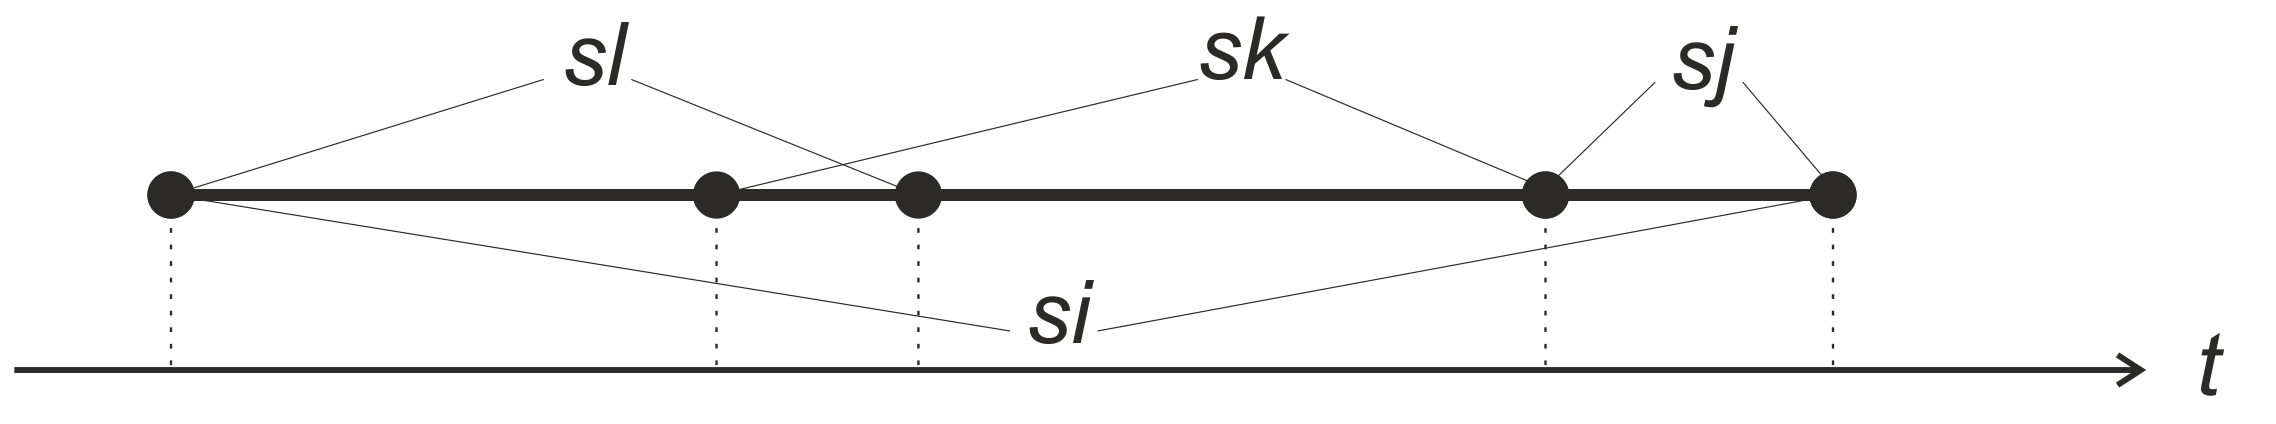
\includegraphics[width=1\linewidth]{figures/sd_temp_entities/img_temporal_union.png}}}

\scnheader{темпоральная декомпозиция*}
\scnrelfrom{типичная семантическая окрестность}{
\scnfilescg{figures/sd_temp_entities/temporal_decomposition.png}}
\scnrelfrom{иллюстрация}{
\scnfileimage{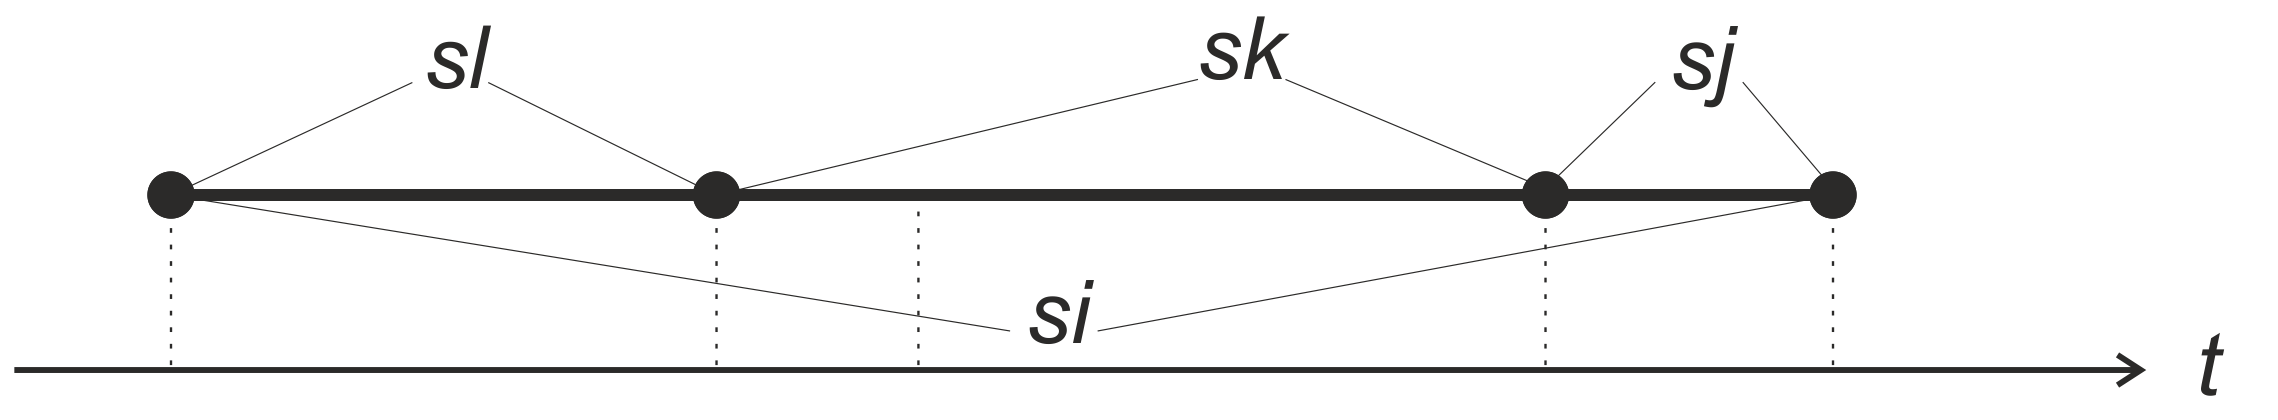
\includegraphics[width=1\linewidth]{figures/sd_temp_entities/img_temporal_decomposition.png}
}}

\scnheader{темпоральная смежность*}
\scnidtf{строгая темпоральная последовательность (без темпорального промежутка)*}
\scnidtf{темпоральная последовательность без промежутка*}
\scnrelfrom{типичная семантическая окрестность}{
\scnfilescg{figures/sd_temp_entities/temporal_adjacency.png}}
\scnrelfrom{иллюстрация}{
\scnfileimage{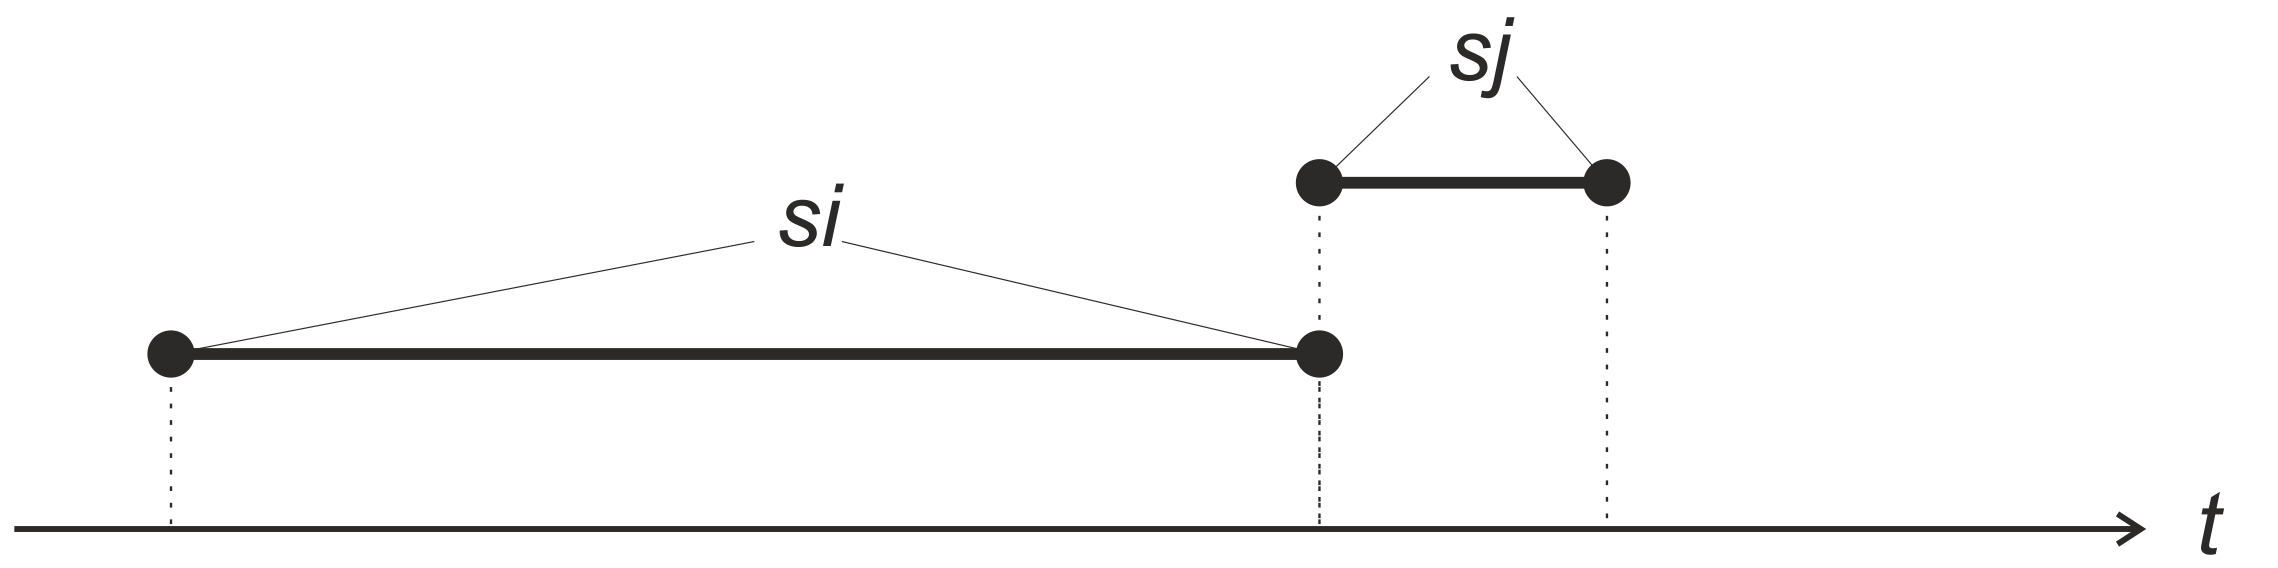
\includegraphics[width=1\linewidth]{figures/sd_temp_entities/img_temporal_adjacency.png}
}}

\scnheader{темпоральная последовательность с промежутком*}
\scnrelfrom{типичная семантическая окрестность}{
\scnfilescg{figures/sd_temp_entities/temporal_sequence_with_intermediate.png}}
\scnrelfrom{иллюстрация}{
\scnfileimage{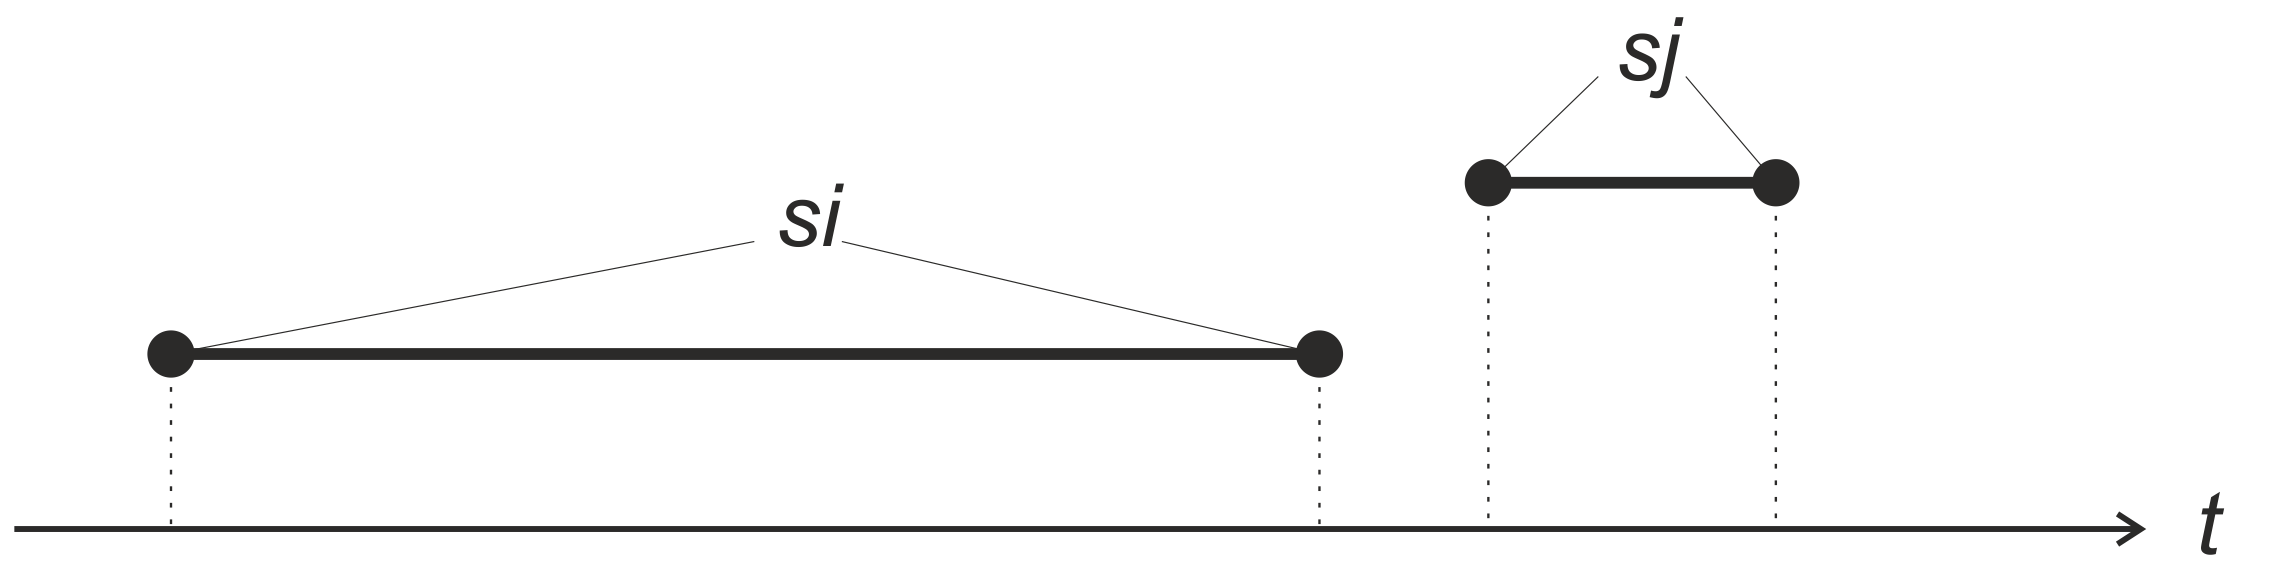
\includegraphics[width=1\linewidth]{figures/sd_temp_entities/img_temporal_sequence_with_intermediate.png}}}

\scnheader{темпоральная последовательность с пересечением*}
\scnrelfrom{типичная семантическая окрестность}{
\scnfilescg{figures/sd_temp_entities/temporal_sequence_with_intersection.png}
}
\scnrelfrom{иллюстрация}{
\scnfileimage{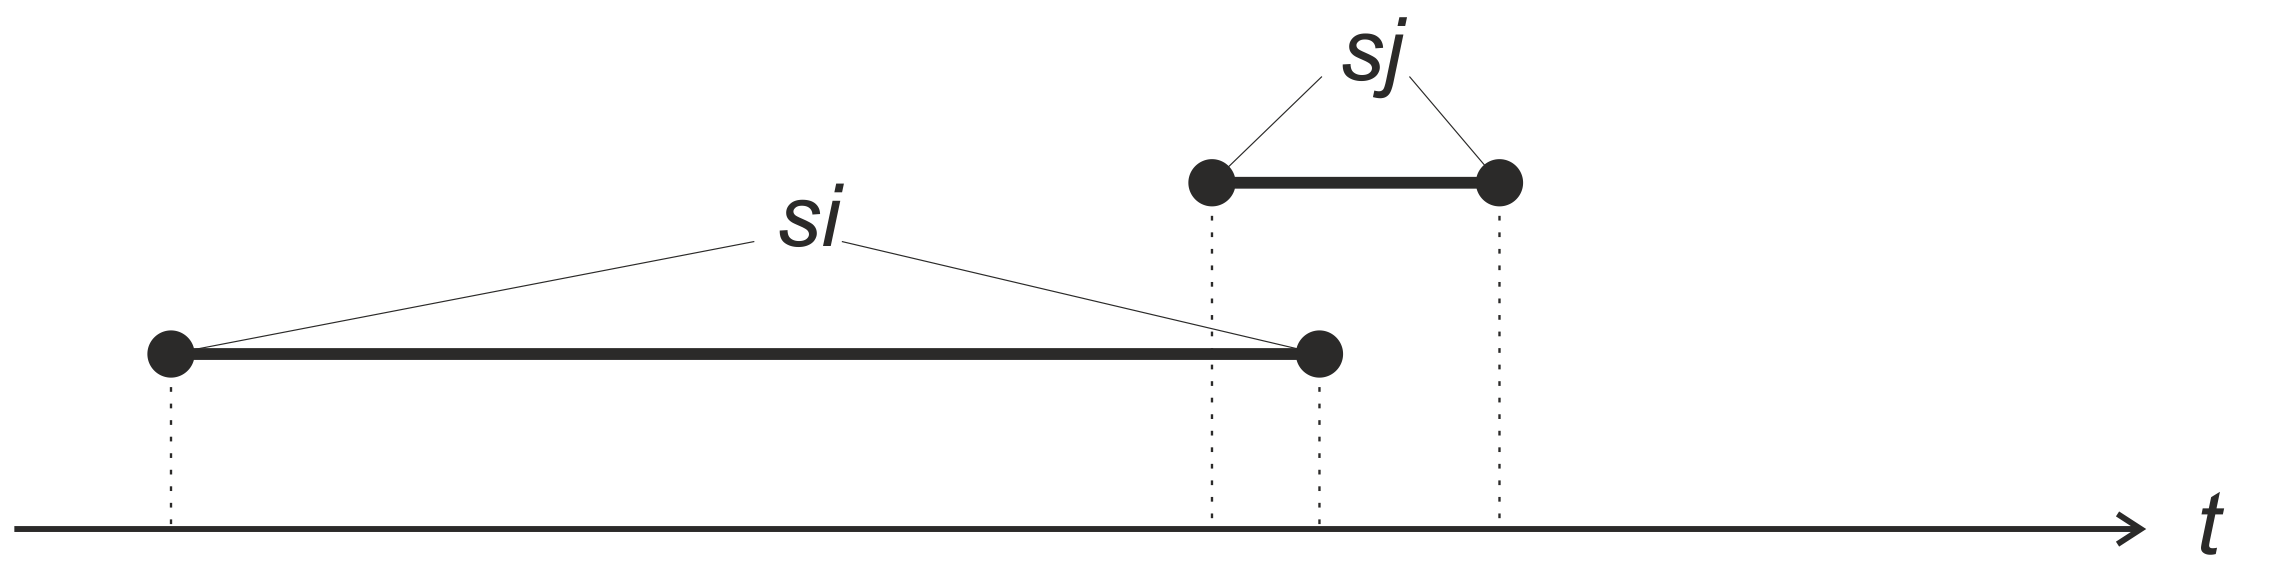
\includegraphics[width=1\linewidth]{figures/sd_temp_entities/img_temporal_cross_sequence.png}
}}

\scnheader{начало}
\scnidtf{класс одновременно начавшихся сущностей}
\scniselement{параметр}
\scnexplanation{Каждый элемент множества \textbf{начало} представляет собой класс \textit{временных сущностей}, у которых совпадает момент начала их существования. Конкретное значение данного \textit{параметра} может быть как \textit{точной величиной}, так и \textit{неточной величиной} или \textit{интервальной величиной}.}
\scnrelfrom{типичная семантическая окрестность}{
\scnfilescg{figures/sd_temp_entities/start.png}}
\scncomment{В данном примере \textbf{\textbf{\textit{ki}}} обозначает класс сущностей, начавших свое существование 19 февраля 2015 года по григорианскому календарю. Конкретные примеры таких сущностей – \textbf{\textit{bi}} и \textbf{\textit{bj}}. \textbf{\textit{ti}} обозначает временную точку григорианского календаря, соответствующую 19 февраля 2015 года.}

\scnheader{завершение}
\scnidtf{конец}
\scnidtf{класс одновременно завершившихся сущностей}
\scniselement{параметр}
\scnexplanation{Каждый элемент множества \textbf{\textit{завершение}} представляет собой класс \textit{временных сущностей}, у которых совпадает конечный момент их существования (момент завершения существования). Конкретное значение данного \textit{параметра} может быть как \textit{точной величиной}, так и \textit{неточной величиной} или \textit{интервальной величиной}.}
\scnrelfrom{типичная семантическая окрестность}{
\scnfilescg{figures/sd_temp_entities/completion.png}}
\scncomment{В данном примере \textbf{\textit{ki}} обозначает класс сущностей, завершивших свое существование 21 февраля 2015 года по григорианскому календарю. Конкретные примеры таких сущностей – \textbf{\textit{bi}} и \textbf{\textit{bj}}. \textbf{\textit{ti}} обозначает временную точку григорианского календаря, соответствующую 21 февраля 2015 года.}

\scnheader{длительность}
\scnidtf{класс временных сущностей, имеющих одинаковую длительность}
\scniselement{параметр}
\scnhaselement{тысячелетие}
\scnhaselement{век}
\scnhaselement{год}
\scnhaselement{месяц}
\scnhaselement{день}
\scnhaselement{час}
\scnhaselement{минута}
\scnhaselement{секунда}
\scnexplanation{Каждый элемент множества \textbf{\textit{длительность}} представляет собой класс \textit{временных сущностей}, у которых совпадает длительность их существования. Конкретное значение данного \textit{параметра} может быть как \textit{точной величиной}, так и \textit{неточной величиной} или \textit{интервальной величиной}.}
\scnrelfrom{типичная семантическая окрестность}{
\scnfilescg{figures/sd_temp_entities/duration.png}}
\scncomment{В данном примере \textbf{\textit{ki}} обозначает класс сущностей, существовавших в течение 2 месяцев. Конкретный пример такой сущности – \textbf{\textit{bi}}.}

\scnheader{тысячелетие}

\scnheader{век}

\scnheader{год}

\scnheader{месяц}

\scnheader{сутки}

\scnheader{час}

\scnheader{минута}

\scnheader{секунда}

\scnheader{номер тысячелетия\scnrolesign}
\scnheader{номер века\scnrolesign}
\scnheader{номер года\scnrolesign}
\scnheader{номер месяца в году\scnrolesign}
\scnheader{номер суток в месяце\scnrolesign}
\scnheader{номер часа в дне\scnrolesign}
\scnheader{номер минуты в часе\scnrolesign}
\scnheader{номер секунды в минуте\scnrolesign}

\scnendstruct \scnendcurrentsectioncomment

\end{SCn}

\scsubsubsection{Предметная область и онтология темпоральных сущностей баз знаний ostis-систем}
\begin{SCn}

\scnsectionheader{\currentname}
\scntext{введение}{Обработка информации в \textit{sc-памяти} (т.е. динамика базы знаний, хранимой в \textit{sc-памяти}) в конечном счете сводится:
\begin{scnitemize}
    \item к появлению в \textit{sc-памяти} новых актуальных \textit{sc-узлов} и \textit{sc-коннекторов};
    \item к логическому удалению актуальных \textit{sc-элементов}, т.е. к переводу их в неактуальное состояние (это необходимо для хранения протокола изменения состояния базы знаний, в рамках которого могут описываться действия по удалению \textit{sc-элементов});
    \item к возврату логически удаленных \textit{sс-элементов} в статус актуальных (необходимость в этом может возникнуть при откате базы знаний к какой-нибудь ее прошлой версии);
    \item к физическому удалению \textit{sc-элементов};
    \item к изменению состояния актуальных (логически не удаленных \textit{sc-элементов}) – \textit{sc-узел} может превратиться в \textit{sc-ребро}, \textit{sc-ребро} может превратиться в \textit{sc-дугу}, \textit{sc-дуга} может поменять направленность, \textit{sc-дуга} общего вида может превратиться в \textit{константную стационарную sc-дугу принадлежности}, и т.д.;
\end{scnitemize}
Подчеркнем, что временный характер самого \textit{sc-элемента} (т.к. он может появиться или исчезнуть) никак не связан с возможно временным характером сущности, обозначаемой этим \textit{sc-элементом}. Т.е. временный характер самого sc-элемента и временный характер сущности, которую он обозначает – абсолютно разные вещи.

Таким образом, следует четко отличать динамику внешнего мира, описываемого базой знаний, а динамику самой базы знаний (динамику внутреннего мира). При этом очень важно, чтобы описание динамики базы знаний также входило в состав каждой базы знаний.

К числу понятий, используемых для описания динамики базы знаний относятся:
\begin{scnitemize}
    \item логически удаленный sc-элемент;
    \item сформированное множество;
    \item вычисленное число;
    \item сформированное высказывание;
\end{scnitemize}}

\scnstartsubstruct

\scnheader{Предметная область темпоральных сущностей базы знаний ostis-системы}
\scnidtf{Предметная область, описывающая динамику базы знаний, хранимой в sc-памяти}
\scniselement{предметная область}
\scnsdmainclasssingle{ситуация}
\scnsdclass{sc-элемент;наcтоящий sc-элемент;логически удаленный sc-элемент;число;невычисленное число;вычисленное число;понятие;основное понятие;неосновное понятие;понятие, переходящее из основного в неосновное;понятие, переходящее из неосновного в основное;специфицированная сущность;недостаточно специфицированная сущность;достаточно специфицированная сущность;средне специфицированная сущность;структура;файл;событие в sc-памяти*;элементарное событие в sc-памяти*;событие добавления sc-дуги, выходящей из заданного sc-элемента*;событие добавления sc-дуги, входящей в заданный sc-элемент*;событие добавления sc-ребра, инцидентного заданному sc-элементу*;событие удаления sc-дуги, выходящей из заданного sc-элемента*;событие удаления sc-дуги, входящей в заданный sc-элемент*;событие удаления sc-ребра, инцидентного заданному sc-элементу*;событие удаления sc-элемента*;событие изменения содержимого файла*}

\scnheader{sc-элемент}
\scnreltoset{разбиение}{наcтоящий sc-элемент;логически удаленный sc-элемент}

\scnheader{наcтоящий sc-элемент}
\scniselement{ситуативное множество}

\scnheader{логически удаленный sc-элемент}
\scniselement{ситуативное множество}

\scnheader{число}
\scnsubdividing{невычисленное число;вычисленное число}

\scnheader{невычисленное число}
\scniselement{ситуативное множество}

\scnheader{вычисленное число}

\scnheader{понятие}
\scnsubdividing{основное понятие;неосновное понятие;понятие, переходящее из основного в неосновное;понятие, переходящее из неосновного в основное}

\scnheader{основное понятие}
\scnidtf{основное понятие для данной ostis-системы}
\scniselement{ситуативное множество}
\scnexplanation{К \textbf{\textit{основным понятиям}} относятся те понятия, которые активно используются в системе и могут быть ключевыми элементами sc-агентов. К \textbf{\textit{основным понятиям}} относятся также все неопределяемые понятия.}

\scnheader{неосновное понятие}
\scnidtf{дополнительное понятие}
\scnidtf{вспомогательное понятие}
\scnidtf{неосновное понятие для данной ostis-системы}
\scniselement{ситуативное множество}
\scnexplanation{Каждое \textbf{\textit{неосновное понятие}} должно быть строго определено на основе \textit{основных понятий}. Такие \textbf{\textit{неосновные понятия}} используются только для понимания и правильного восприятия вводимой информации, в том числе, для выравнивания онтологий. Ключевым элементом \textit{sc-агентов} \textbf{\textit{неосновные понятия}} быть не могут.}
\scntext{правило идентификации экземпляров}{В случае, когда некоторое понятие полностью перешло из \textit{основных понятий} в неосновные, то есть стало \textbf{\textit{неосновным понятием}}, и соответствующее ему \textit{основное понятие} (через которое оно определяется) в рамках некоторого внешнего языка имеет одинаковый с ним основной идентификатор, то к идентификатору \textbf{\textit{неосновного понятия}} спереди добавляется знак \#. Если при этом соответствуюшее \textit{основное понятие} имеет в идентификаторе знак \$, добавленный в процессе перехода, то этот знак удаляется. Если указанные понятия имеют разные основные идентификаторы в рамках этого внешнего языка, то никаких дополнительных средств идентификации не используется.

Например:\\
\textit{\#трансляция sc-текста}\\
\textit{\#scp-программа}}

\scnheader{понятие, переходящее из основного в неосновное}
\scniselement{ситуативное множество}

\scnheader{понятие, переходящее из неосновного в основное}
\scniselement{ситуативное множество}
\scntext{правило идентификации экземпляров}{В случае, когда текущее \textit{основное понятие} и соответствующее ему \textbf{\textit{понятие, переходящее из неосновного в основное}} в рамках некоторого внешнего языка имеют одинаковый основной идентификатор, то к идентификатору понятия, переходящего из неосновного в основное спереди добавляется знак \$. Если указанные понятия имеют разные основные идентификаторы в рамках этого внешнего языка, то никаких дополнительных средств идентификации не используется.

Например:\\
\textit{\$трансляция sc-текста}\\
\textit{\$scp-программа}}

\scnheader{специфицированная сущность}
\scnsubdividing{недостаточно специфицированная сущность;достаточно специфицированная сущность;средне специфицированная сущность}

\scnheader{недостаточно специфицированная сущность}

\scnheader{достаточно специфицированная сущность}
\scnexplanation{К \textbf{\textit{достаточно специфицированным сущностям}} предъявляются следующие требования:
\begin{scnitemize}
    \item если сущность не является понятием, то для нее должны быть указаны
    \begin{scnenumerate}
    \item различные варианты обозначающих ее внешних знаков;
    \item классы, которым она принадлежит;
    \item связки, которыми она связана с другими сущностями (с указанием соответствующего отношения);
    \item значения параметров, которыми она обладает;
    \item те разделы базы знаний, в которых указанная сущность является ключевой;
    \item предметные области, в которые данная сущность входит.
    \end{scnenumerate}
    \item если специфицированная сущность является понятием, то для нее должны быть указаны:
    \begin{scnenumerate}
    \item различные варианты внешних обозначений этого понятия;
    \item предметные области, в которых это понятие исследуется;
    \item определение понятия;
    \item пояснения
    \item разделы базы знаний, в которых это понятие является ключевым;
    \item типичная семантическая окрестность – пример экземпляра понятия.
    \end{scnenumerate}
\end{scnitemize}}

\scnheader{средне специфицированная сущность}

\scnheader{структура}
\scnsubdividing{сформированная структура;несформированная структура}
\scnsubdividing{недостаточно сформированная структура;достаточно сформированная структура;структура, имеющая средний уровень сформированности}

\scnheader{файл}
\scnsubdividing{недостаточно сформированный внутренний файл;достаточно сформированный внутренний файл;внутренний файл, имеющий средний уровень сформированности}

\scnheader{событие в sc-памяти*}
\scnrelto{включение}{событие*}

\scnheader{элементарное событие в sc-памяти*}
\scnrelto{включение}{событие в sc-памяти*}
\scnexplanation{Под \textbf{\textit{элементарным событием в sc-памяти*}} понимается \textit{событие*}, соответствующее некоторому действию в \textit{sc-памяти}, в результате выполнения которого изменяется состояние только одного \textit{sc-элемента}.}
\scnsubdividing{событие добавления sc-дуги, выходящей из заданного sc-элемента*
;событие добавления sc-дуги, входящей в заданный sc-элемент*;событие добавления sc-ребра, инцидентного заданному sc-элементу*;событие удаления sc-дуги, выходящей из заданного sc-элемента*;событие удаления sc-дуги, входящей в заданный sc-элемент*;событие удаления sc-ребра, инцидентного заданному sc-элементу*;событие удаления sc-элемента*;событие изменения содержимого файла*}

\scnheader{событие добавления sc-дуги, выходящей из заданного sc-элемента*}

\scnheader{событие добавления sc-дуги, входящей в заданный sc-элемент*}

\scnheader{событие добавления sc-ребра, инцидентного заданному sc-элементу*}

\scnheader{событие удаления sc-дуги, выходящей из заданного sc-элемента*}

\scnheader{событие удаления sc-дуги, входящей в заданный sc-элемент*}

\scnheader{событие удаления sc-ребра, инцидентного заданному sc-элементу*}

\scnheader{событие удаления sc-элемента*}

\scnheader{событие изменения содержимого файла*}

\scnendstruct

\end{SCn}

\scsubsubsection{Предметная область и онтология действий, задач, планов, протоколов и методов}
\label{sec:sd_actions}
\begin{SCn}

\bigskip
\scnfragmentcaptiontext{Понятие класса действий и метода}

\scnheader{класс действий}
\scnrelto{семейство подклассов}{действие}
\scnidtfexp{\uline{максимальное} множество аналогичных (похожих в определенном смысле) действий, для которого существует (но не обязательно известный в текущий момент) по крайней мере один \textbf{метод} (или средство), обеспечивающий выполнение \uline{любого} действия из указанного множества действий} 
\scnidtf{множество однотипных действий}
\scnsuperset{класс элементарных действий}
\scnsuperset{класс легко выполнимых сложных действий}
\scnnote{Тот факт, что каждому выделяемому \textit{классу действий} соответствует по крайней мере один общий для них \textit{метод} выполнения этих \textit{действий}, означает то, что речь идет о \uline{семантической} "кластеризации"{} множества \textit{действий}, т.е. о выделении \textit{классов действий} по признаку \uline{семантической близости} (сходства) \textit{действий}, входящих в состав выделяемого \textit{класса действий}. При этом прежде всего учитывается аналогичность (сходство) \textit{исходных ситуаций} и \textit{целевых ситуаций} рассматриваемых \textit{действий}, т.е. аналогичность \textit{задач}, решаемых в результате выполнения соответствующих \textit{действий}. Поскольку одна и та же \textit{задача} может быть решена в результате выполнения нескольких \uline{разных} \textit{действий}, принадлежащих \uline{разным} \textit{классам действий}, следует говорить не только о \textit{классах действий} (множествах аналогичных действий), но и о \textbf{\textit{классах задач}} (о множествах аналогичных задач), решаемых этими \textit{действиями}. Так, например, на множестве \textit{классов действий} заданы следующие \textit{отношения}:
	\begin{scnitemize}
	\item \textit{отношение}, каждая связка которого связывает два разных (непересекающихся) \textit{класса действий}, осуществляющих решение одного и того же \textit{класса задач};
	\item \textit{отношение}, каждая связка которого связывает два разных \textit{класса действий}, осуществляющих решение разных \textit{классов задач}, один из которых является \textit{надмножеством} другого.
	\end{scnitemize}}

\scnheader{класс элементарных действий}
\scnidtf{множество элементарных действий, указание принадлежности которому является \uline{необходимым} и достаточным условием для выполнения этого действия}
\scnnote{Множество всевозможных элементарных действий, выполняемых каждым субъектом, должно быть \uline{разбито} на классы элементарных действий.}

\scnheader{класс легковыполнимых сложных действий}
\scnidtf{множество сложных действий, для которого известен и доступен по крайней мере один \textbf{\textit{метод}}, интерпретация которого позволяет осуществить полную (окончательную, завершающуюся элементарными действиями) декомпозицию на поддействия \uline{каждого} сложного действия из указанного выше множества}
\scnidtf{множество всех сложных действий, выполнимых с помощью известного \textit{метода}, соответствующего этому множеству}

\scnheader{спецификация*} 
\scnsuperset{сужение отношения по первому домену*(спецификация*; класс действий)*}
	\scnaddlevel{1}
  	\scnidtftext{часто используемый sc-идентификатор}{спецификация класса действий*}
  	\scnsubdividing{\textbf{обобщенная формулировка задач соответствующего класса*}\\
  	\scnaddlevel{1}
  	\scnsubdividing{\textbf{обобщенная декларативная формулировка задач соответствующего класса*}
  	;\textbf{обобщенная процедурная формулировка задач соответствующего класса*}}
  	\scnaddlevel{-1}
  	;\textbf{метод*}\\
  	\scnaddlevel{1}
  	\scnidtf{метод решения задач заданного класса*}
  	\scnidtf{метод выполнения действий соответствующего (заданного) класса*}
  	\scnsubdividing{\textbf{процедурный метод выполнения действий соответствующего класса*}\\
  	\scnaddlevel{1}
  	\scnidtf{обобщенный план выполнения действий заданного класса*}
  	\scnaddlevel{-1}
  	;\textbf{декларативный метод выполнения действий соответствующего класса*}\\
  	\scnaddlevel{1}
  	\scnidtf{обобщенная декларативная спецификация выполнения действий заданного класса*}
  	\scnaddlevel{-1}}
  	\scnaddlevel{-1}}
  	\scnaddlevel{-1}

\scnheader{класс задач}
\scnidtf{множество аналогичных действий}
\scnidtf{множество задач, для которого можно построить обобщенную формулировку задач, соответствующую всему этому множеству задач}
\scnnote{Каждая \textit{обобщенная формулировка задач соответствующего класса} по сути есть не что иное, как строгое логическое определение указанного класса задач.}

\scnheader{класс действий}
\scnsubdividing{\textbf{класс действий, однозначно задаваемый решаемым классом задач}\\
	\scnaddlevel{1}
	\scnidtf{\textit{класс действий}, обеспечивающих решение соответствующего \textit{класса задач} и использующих при этом любые, самые разные \textit{методы} решения задач этого класса}
	\scnaddlevel{-1}
	;\textbf{класс действий, однозначно задаваемый используемым методом решения задач}}

\scnheader{метод}
\scnrelto{второй домен}{метод*}
\scnidtf{описание того, \uline{как} может быть выполнено любое или почти любое действие, принадлежащее соответствующему классу действий}
\scnidtf{метод решения соответствующего класса задач, обеспечивающий решение любой или большинства задач указанного класса}
\scnidtf{обобщенная спецификация выполнения действий соответствующего класса}
\scnidtf{обобщенная спецификация решения задач соответствующего класса}
\scnidtf{программа решения задач соответствующего класса, которая может быть как процедурной, так и декларативной (непроцедурной)}
\scnidtf{знание о том, как можно решать задачи соответствующего класса}
\scnsubset{знание}
\scniselement{вид знаний}

\scnidtf{способ}
\scnidtf{знание о том, как надо решать задачи соответствующего класса задач (множества эквивалентных (однотипных, похожих) задач)}
\scnidtf{метод (способ) решения некоторого (соответствующего) класса задач}
\scnsubset{процедурная программа}
	\scnaddlevel{1}
	\scnsubset{алгоритм}
	\scnaddlevel{-1}
\scnidtf{информация (знание), достаточная для того, чтобы решить любую \textit{задачу}, принадлежащую соответствующему \textit{классу задач} с помощью соответствующей \textit{модели решения задач}}
\scnnote{В состав спецификации каждого \textit{класса задач} входит описание способа "привязки"{} \textit{метода} к исходным данным конкретной \textit{задачи}, решаемой с помощью этого \textit{метода}. Описание такого способа "привязки"{} включает в себя:
	\begin{scnitemize}
	\item набор переменных, которые входят как в состав \textit{метода}, так и в состав \textit{обобщенной формулировки задач соответствующего класса} и значениями которых являются соответствующие элементы исходных данных каждой конкретной решаемой задачи;
	\item часть \textit{обобщенной формулировки задач} того класса, которому соответствует рассматриваемый \textit{метод}, являющихся описанием \uline{условия применения} этого \textit{метода}.
	\end{scnitemize}
\bigskip
Сама рассматриваемая "привязка"{} \textit{метода} к конкретной \textit{задаче}, решаемой с помощью этого \textit{метода} осуществляется путем \uline{поиска} в \textit{базе знаний} такого фрагмента, который удовлетворяет условиям применения указанного \textit{метода}. Одним из результатов такого поиска и является установление соответствия между указанными выше переменными используемого \textit{метода} и значениями этих переменных в рамках конкретной решаемой \textit{задачи}. 

Другим вариантом установления рассматриваемого соответствия является явное обращение (вызов, call) соответствующего \textit{метода} (программы) с явной передачей соответствующих параметров. Но такое не всегда возможно, т.к. при выполнении процесса решения конкретной \textit{задачи} на основе декларативной спецификации выполнения этого действия нет возможности установить:
	\begin{scnitemize}
	\item когда необходимо инициировать вызов (использование) требуемого \textit{метода};
	\item какой конкретно \textit{метод} необходимо использовать;
	\item какие параметры, соответствующие конкретной инициируемой \textit{задачи}, необходимо передать для "привязки"{} используемого \textit{метода} к этой \textit{задаче}.
	\end{scnitemize}
	

Процесс "привязки"{} \textit{метода} решения \textit{задач} к конкретной \textit{задаче}, решаемой с помощью этого \textit{метода}, можно также представить как процесс, состоящий из следующих этапов:
	\begin{scnitemize}
	\item построение копии используемого \textit{метода};
	\item склеивание основных (ключевых) переменных используемого \textit{метода} с основными параметрами конкретной решаемой \textit{задачи}.
	\end{scnitemize}

В результате этого на основе рассматриваемого \textit{метода} используемого в качестве образца (шаблона) строится спецификация процесса решения конкретной задачи -- процедурная спецификация (\textit{план}) или декларативная.}
\scnnote{Заметим, что \textit{методы} могут использоваться даже при построении \textit{планов} решения конкретных \textit{задач}, в случае, когда возникает необходимость многократного повторения неких цепочек \textit{действий} при априори неизвестном количестве таких повторений. Речь идет о различного вида \textbf{циклах}, которые являются простейшим видом процедурных \textit{методов} решения задач, многократно используемых (повторяемых) при реализации \textit{планов} решения некоторых \textit{задач}.}

\scnheader{эквивалентность задач*}
\scnidtf{быть эквивалентной задачей*}
\scniselement{отношение}
\scntext{определение}{Задачи являются эквивалентными в том и только в том случае, если они могут быть решены путем интерпретации одного и того же \textit{метода} (способа), хранимого в памяти кибернетической системы.}
\scnnote{Некоторые \textit{задачи} могут быть решены разными \textit{методами}, один из которых, например, является обобщением другого.}

\scnheader{отношение, заданное на множестве методов}
\scnhaselement{подметод*}
	\scnaddlevel{1}
	\scnidtf{подпрограмма*}
	\scnidtf{быть методом, использование которого (обращение к которому) предполагается при реализации заданного метода*}
	\scnrelboth{следует отличать}{частный метод*}
	\scnaddlevel{1}
	\scnidtf{быть методом, обеспечивающим решение класса задач, который является подклассом задач, решаемых с помощью заданного метода*}
	\scnaddlevel{-1}

\scnheader{стратегия решения задач}
\scnsubset{метод}
\scnidtf{метаметод решения задач, обеспечивающий либо поиск одного релевантного известного метода, либо синтез целенаправленной последовательности аций применения в общем случае различных известных методов}
\scnnote{Можно говорить об универсальном метаметоде (универсальной стратегии) решения задач, объясняющем всевозможные частные стратегии.}
\scnexplanation{Можно говорить о нескольких глобальных \textit{стратегиях решения информационных задач} в базах знаний. Пусть в базе знаний появился знак инициированного действия с формулировкой соответствующей информационной цели, т.е. цели, направленной только на изменение состояния базы знаний. И пусть текущее состояние базы знаний не содержит контекста (исходных данных), достаточного для достижения указанной выше цели, т.е такого контекста, для которого в доступном пакете (наборе) методов (программ) имеется метод (программа), использование которого позволяет достигнуть указанную выше цель. Для достижения такой цели, контекст( исходные данные) которой недостаточен, существует три подхода (три стратегии): 
	\begin{scnitemize}
	\item декомпозиция (сведение изначальной цели к иерархической системе и/или подцелей (и/или подзадач) на основе анализа текущего состояния базы знаний и анализа того, чего в базе знаний не хватает для использования того или иного метода.) 
	
	При этом наибольшее внимание уделяется методам, для создания условий использования которых требуется меньше усилий. В конечном счете мы должны дойти (на самом нижнем уровне иерархии) до подцелей, контекст которых достаточен для применения одного из имеющихся методов (программ) решения задач;
	\item генерация новых знаний в семантической окрестности формулировки изначальной цели с помощью \uline{любых} доступных методов в надежде получить такое состояние базы знаний, которое будет содержать нужный контекст (достаточные исходные данные) для достижения изначальной цели с помощью какого-либо имеющегося метода решения задач;
	\item комбинация первого и второго подхода.
	\end{scnitemize}
Аналогичные стратегии существуют и для поиска пути решения задач, решаемых во внешней среде.}
\end{SCn}
\begin{SCn}

\scnsectionheader{\currentname}

\scnstartsubstruct

\begin{SCn}
	
\scniselement{раздел}
\scniselement{предметная область и онтология}
\scnreltovector{конкатенация сегментов}{Уточнение понятия воздействия и понятия действия. Типология воздействий и действий;Уточнение понятия задачи. Типология задач;Уточнение семейства параметров и отношений, заданных на множестве воздействий, действий и задач;Предметная область и онтология субъектно-объектных спецификаций воздействий;Уточнение понятий плана сложного действия, класса задач, метода; Уточнение понятия навыка, понятия класса методов и понятия модели решения задач;Уточнение понятия деятельности, понятия вида деятельности и понятия технологии}

\scnhaselementlist{исследуемый класс первичных объектов исследования}{
воздействие\\
	\scnaddlevel{1}
	\scnidtf{\textit{процесс} воздействия одних \textit{сущностей} на другие}
	\scnsubset{процесс}
	\scnaddlevel{-1}
;действие\\
	\scnaddlevel{1}
	\scnidtf{\textit{процесс}, "осознанно"{} и целенаправленно выполняемый (управляемый) некоторой \textit{кибернетической системой}}
	\scnsubset{воздействие}
	\scnsubset{процесс}
	\scnaddlevel{-1}
\bigskip
;неосознанное воздействие
\bigskip
;действие, выполняемое в памяти субъекта действия
;действие, выполняемое во внешней среде субъекта действия
;рецепторное действие\\
	\scnaddlevel{1}
	\scnidtf{действие, выполняемое рецептором субъекта действия}
	\scnaddlevel{-1}
;эффекторное действие\\
	\scnaddlevel{1}
	\scnidtf{действие, выполняемое эффектором субъекта действия}
	\scnaddlevel{-1}
\bigskip
;элементарное действие \\
	\scnaddlevel{1}
	\scnidtf{действие, выполнение которого не требует его декомпозиции на взаимосвязанные поддействия}
	\scnaddlevel{-1}
;сложное действие
;легко выполнимое сложное действие\\
	\scnaddlevel{1}
	\scnidtf{сложное действие, которое известно, как выполнять}
	\scnaddlevel{-1}
;интеллектуальное действие\\
	\scnaddlevel{1}
	\scnidtf{сложное действие, для которого априори не известно, как его выполнять}
	\scnaddlevel{-1}
\bigskip
;индивидуальное действие\\
	\scnaddlevel{1}
	\scnidtf{действие, выполняемое индивидуальной кибернетической системой}
	\scnaddlevel{-1}
;коллективное действие\\
	\scnaddlevel{1}
	\scnidtf{действие, выполняемое коллективом кибернетических систем (многоагентной системой)}
	\scnaddlevel{-1}
\bigskip
;планируемое действие
;инициированное действие
;выполняемое действие
	\scnaddlevel{1}
	\scnidtf{активное действие}
	\scnaddlevel{-1}
;прерванное действие
	\scnaddlevel{1}
	\scnidtf{выполняемое действие, находящееся в состоянии прерывания}
	\scnaddlevel{-1}
;выполненное действие
;отмененное действие
\bigskip
;действие с очень высоким приоритетом
;действие с высоким приоритетом
;действие со средним приоритетом
;действие с низким приоритетом
;действие с очень низким приоритетом}
\bigskip

\scnhaselementlist{исследуемый класс классов первичных объектов исследования}{
осмысленность воздействия\scnsupergroupsign
;длительность воздействия\scnsupergroupsign
;место выполнения действия\scnsupergroupsign
;функциональная сложность действия\scnsupergroupsign
;многоагентность действия\scnsupergroupsign\\
	\scnaddlevel{1}
	\scnidtf{коллективность субъекта действия}
	\scnaddlevel{-1}
;текущее состояние действия\scnsupergroupsign
;приоритет действия\scnsupergroupsign\\
	\scnaddlevel{1}
	\scnidtf{важность действия\scnsupergroupsign}
	\scnaddlevel{-1}
;срочность действия\scnsupergroupsign
\bigskip
;класс действий
;класс функционально эквивалентных действий\scnsupergroupsign
;класс логически эквивалентных действий\scnsupergroupsign
;класс семантических эквивалентных задач\scnsupergroupsign
;класс логически эквивалентных задач\scnsupergroupsign
;класс задач, для которого существует общий метод их решения\scnsupergroupsign
;класс аналогичных семантически элементарных процессов воздействия\scnsupergroupsign\\
	\scnaddlevel{1}
	\scnidtf{класс однотипных семантически элементарных воздействий\scnsupergroupsign}
	\scnaddlevel{-1}}

	
\scnhaselementlist{исследуемый класс классов}
{отношение, заданное на множестве* (действие)\\
	\scnaddlevel{1}
	\scnidtf{отношение, заданное на множестве действий}
	\scnaddlevel{-1}
;отношение, заданное на множестве* (задача)
;параметр, заданный на множестве* (действие)
;параметр, заданный на множестве* (задача)}
\scnaddlevel{1}
\scnsourcecommentpar{Здесь указаны классы классов, которые не являются классами классов \uline{первичных} объектов исследования}
\scnaddlevel{-1}
\bigskip

\scnhaselementlist{исследуемое отношение, заданное на множестве первичных объектов исследования}{воздействующая сущность\scnrolesign
;воздействуемая сущность\scnrolesign
;посредник\scnrolesign
;медиатор\scnrolesign
;субъект\scnrolesign\\
	\scnaddlevel{1}
	\scnidtf{быть субъектом заданного действия}
	\scnaddlevel{-1}
;спецификация воздействия*\\
	\scnaddlevel{1}
	\scnsuperset{спецификация действия*}
	\scnaddlevel{-1}
;спецификация действия*\\
	\scnaddlevel{1}
	\scnsuperset{задача*}
		\scnaddlevel{1}
		\scnsubdividing{декларативная формулировка задачи*;процедурная формулировка задачи*}
		\scnaddlevel{-1}
		\scnsuperset{план сложного действия*}
		\scnsuperset{декларативная спецификация выполнения сложного действия*}
		\scnsuperset{протокол*}
		\scnsuperset{результативная часть протокола*}
	\scnaddlevel{-1}
;декларативная формулировка задачи*
;процедурная формулировка задачи*
;план сложного действия*
;декларативная спецификация выполнения сложного действия*
;протокол*
;результативная часть протокола*}
\bigskip

\scnhaselementlist{исследуемое отношение}{спецификация класса действий*
;спецификация метода*
;спецификация класса методов*
;спецификация деятельности*
;спецификация вида деятельности*
}
\scnaddlevel{1}
	\scnsourcecommentpar{Здесь указаны исследуемые отношения, которые заданы не на множестве первичных объектов исследования}
\scnaddlevel{-1}
\bigskip

\scnhaselementlist{исследуемый класс структур, специфицирующих первичные объекты исследования}{
задача\\
	\scnaddlevel{1}
	\scnidtf{формулировка задачи}
	\scnidtf{спецификация действия}
	\scnidtf{структура (sc-конструкция), содержащая в идеале достаточную информацию для выполнения соответствующего (специфицируемого) действия}
	\scnaddlevel{-1}
;декларативная формулировка задачи\\
	\scnaddlevel{1}
	\scnidtf{семантическая спецификация действия}
	\scnaddlevel{-1}
;процедурная формулировка задачи\\
	\scnaddlevel{1}
	\scnidtf{функциональная спецификация действия}
	\scnaddlevel{-1}
;план сложного действия\\
	\scnaddlevel{1}
	\scnidtf{план выполнения сложного действия}
	\scnaddlevel{-1}
;процедурный план сложного действия
;непроцедурный план сложного действия\\
	\scnaddlevel{1}
	\scnidtf{декларативный план сложного действия}
	\scnidtf{иерархическая система подзадач заданной сложной задачи}
	\scnaddlevel{-1}}
\bigskip

\scnhaselementlist{исследуемый класс структур}{метод\\
	\scnaddlevel{1}
	\scnidtf{спецификация класса сложных действий}
	\scnaddlevel{-1}
;денотационная семантика метода
;операционная семантика метода
;навык
;модель решения задач
;технология}
\scnaddlevel{1}
	\scnsourcecommentpar{Здесь указаны классы структур, не являющихся спецификациями первичных объектов исследования}
\scnaddlevel{-1}
\bigskip

\scnhaselementlist{вводимое, но не исследуемое понятие}
{действие, выполняемое в памяти ostis-системы
;действие, выполняемое ostis-системой в своей внешней среде
;рецептурное действие ostis-системы
;эффекторное действие ostis-системы
;sc-агент\\
	\scnaddlevel{1}
	\scnidtf{внутренний субъект ostis-системы}
	\scnidtf{субъект, реализующий действия, выполняемые в памяти ostis-системы}
	\scnaddlevel{-1}}
\scnaddlevel{1}
	\scnsourcecommentpar{Здесь указаны понятия, исследуемые в предметной области (и соответствующей онтологии), которая является \uline{частной} по отношению к заданной и которая наследует все свойства заданной предметной области и онтологии}
\scnaddlevel{-1}
\bigskip

\scnhaselementlist{используемое понятие, исследуемое в другой предметной области и онтологии}{
кибернетическая система\\
	\scnaddlevel{1}
	\scnidtf{сущность, обладающая способностью быть субъектом различного вида действий}
	\scnaddlevel{-1}
;компьютерная система\\
	\scnaddlevel{1}
	\scnidtf{искусственная кибернетическая система}
	\scnsubset{кибернетическая система}
	\scnaddlevel{-1}
;интеллектуальная компьютерная система\\
	\scnaddlevel{1}
	\scnsubset{компьютерная система}
	\scnsuperset{ostis-система}
	\scnaddlevel{-1}
;человек\\
	\scnaddlevel{1}
	\scnsubset{кибернетическая система}
	\scnaddlevel{-1}
;ostis-система
;спецификация*
	\scnaddlevel{1}
	\scnidtf{быть спецификацией (описанием, семантической окрестностью заданной сущности*)}
	\scnidtf{семантическая окрестность*}
	\scnaddlevel{-1}}


\scnheader{следует отличать*}
\scnhaselementset{
	\scnmakevectorlocal{действие;класс действий};
	\scnmakevectorlocal{метод;класс методов};
	\scnmakevectorlocal{деятельность;вид деятельности}
}
\scnaddlevel{1}
\scnsubset{семейство подклассов*}
\scnnote{Все сущности, принадлежащие рассмотренным \textit{понятиям}, требуют достаточно детальной \textit{спецификации}. При этом не следует путать сами сущности и их \textit{спецификации}. Так, например, не следует путать \textit{действие} и \textit{задачу}, которая специфицирует (уточняет) это \textit{действие}. Особое место среди указанных понятий занимает понятие \textit{метода}, т.к. каждый конкретный \textit{метод}, с одной стороны, является \textit{спецификацией} соответствующего \textit{класса действий}, а, с другой стороны, сам нуждается в \textit{спецификации}, которая уточняет либо \textit{декларативную семантику} этого \textit{метода} (т.е. обобщенную декларативную формулировку класса задач, решаемых с помощью этого \textit{метода}), либо \textit{операционную семантику} этого \textit{метода}, (т.е. множество \textit{методов}, обеспечивающих \textit{интерпретацию} данного специфицируемого \textit{метода}) и тем самым "преобразует"{} специфицируемый \textit{метод} в \textit{навык}.}
\scnaddlevel{-1}


\scnheader{следует отличать*}
\scnhaselementvector{первый домен*(спецификация*)\\
\scnaddlevel{1}
\scnidtf{специфицируемая сущность}
\scnidtf{сущность, использование которой требует вполне определенной ее спецификации}
\scnsuperset{действие}
\scnsuperset{класс действий}
\scnsuperset{метод}
\scnsuperset{класс методов}
\scnsuperset{деятельность}
\scnsuperset{вид деятельности}
\scnaddlevel{-1};
второй домен*(спецификация*)\\
\scnaddlevel{1}
\scnidtf{спецификация}
\scnsuperset{задача}
\scnaddlevel{1}
\scnsuperset{декларативная формулировка задачи}
	\scnaddlevel{1}
	\scnidtf{семантическая формулировка задачи}
	\scnaddlevel{-1}
\scnsuperset{процедурная формулировка задачи}
	\scnaddlevel{1}
	\scnidtf{функциональная формулировка задачи}
	\scnaddlevel{-1}
\scnaddlevel{-1}
\scnsuperset{план действия}
	\scnaddlevel{1}
	\scnidtf{план}
	\scnidtf{план выполнения действия}
	\scnaddlevel{-1}
\scnsuperset{декларативная спецификация выполнения действий}
	\scnaddlevel{1}
	\scnidtf{иерархическая система подзадач}
	\scnaddlevel{-1}
\scnsuperset{протокол}
\scnsuperset{результативная часть протокола}
\scnsuperset{обобщенная декларативная формулировка класса задач}
\scnsuperset{метод}
\scnsuperset{декларативная семантика метода}
\scnsuperset{операционная семантика метода}
\scnsuperset{модель решения задач}
\scnaddlevel{-1}
}
\scnaddlevel{1}
\scnnote{
При этом следует отличать:
\begin{scnitemize}
\item спецификацию конкретного \textit{действия} (\textit{задачу}, \textit{план}, \textit{декларативную спецификацию выполнения действия}, \textit{протокол}, \textit{результативную часть протокола});
\item спецификацию конкретной \textit{деятельности} (\textit{контекст}*, \textit{множество используемых методов}*);
\item спецификацию \textit{класса действий} (\textit{обобщенную декларативную формулировку класса задач}, \textit{метод});
\item спецификацию \textit{вида деятельности} (\textit{технологию});
\item спецификацию \textit{метода} (\textit{декларативную семантику метода}, \textit{операционную семантику метода});
\item спецификацию \textit{класса методов} (\textit{модель решения задач}).
\end{scnitemize}
}
\scnaddlevel{-1}


\scnheader{следует отличать*}
\scnhaselementset{
	\scnmakevectorlocal{действие;класс действий, метод};
	\scnmakevectorlocal{деятельность;вид деятельности, технология}
}

\end{SCn}

\begin{SCn}
	
\scnsegmentheader{Уточнение понятия воздействия и понятия действия. Типология воздействий и действий}

\scnstartsubstruct

\scniselement{сегмент базы знаний}

\scnheader{воздействие}
\scnidtf{\textit{процесс} воздействия одной сущности (или некоторого множества \textit{сущностей}) на другую \textit{сущность} (или на некоторое множество других \textit{сущностей})}
\scnidtf{\textit{процесс}, в котором могут быть явно выделены хотя бы одна воздействующая сущность (\textit{субъект воздействия\scnrolesign}) и хотя бы одна \textit{сущность}, на которую осуществляется воздействие (\textit{субъект воздействия\scnrolesign})}

\scnheader{воздействие}
\scnsubset{процесс}
\scnaddlevel{1}
\scnidtf{динамическая структура}
\scnaddlevel{-1}
\scnnote{Поскольку \textit{воздействия} являются частным видом \textit{процессов}, воздействиями наследуются все свойства \textit{процессов}. Смотрите Раздел \textit{Предметная область и онтология структур}). В частности, используются все \textit{параметры}, заданные на множестве \textit{процессов}, например, \textit{длительность*}, \textit{момент начала процесса*}, \textit{момент завершения процесса\scnsupergroupsign}}

\scnheader{процесс}
\scnrelfrom{покрытие}{длительность\scnsupergroupsign\\
	\scneqtoset{краткосрочный процесс;среднесрочный процесс;долгосрочный процесс; перманентный процесс}
	\scnnote{Длительность различных процессов можно уточнять до любой необходимой точности, используя различные единицы измерения длительности (с точностью до секунд, минут, часов, дней, месяцев, лет, столетий и т.д.). Кроме того, можно ссылаться на процессы, длительность (время жизни) которых соизмерима с рассматриваемым процессом.}
}

\scnheader{действие}
\scnsubset{воздействие}
\scnaddlevel{1}
\scnsubset{процесс}
\scnaddlevel{-1}
\scnidtf{\textit{воздействие}, в котором \textit{воздействующая сущность\scnrolesign} осуществляет \textit{воздействие} "осознанно"{}, целенаправленно}
\scnidtf{целенаправленный процесс, выполняемый одним или несколькими субъектами (кибернетическими системами) с возможным применением некоторых инструментов}
\scnidtf{акция}
\scnidtf{акт}
\scnidtf{операция}
\scnidtf{\uline{процесс} воздействия некоторой (возможно, коллективной) сущности (субъекта воздействия) на некоторую одну или несколько сущностей (объектов воздействия - исходных объектов (аргументов) или целевых (создаваемых или модифицируемых) объектов)}
\scnidtf{осознанное воздействие}
\scnidtf{активное воздействие}
\scnidtf{целеноправленный ("осознанный") процесс, выполняемый (управляемый, реализуемый) неким субъектом}
\scnidtf{акция реализации некоторого замысла}
\scnidtf{преднамеренная акция}
\scnidtf{работа}
\scnidtf{процесс выполнения некоторой задачи}
\scnidtf{дело}
\scnidtf{целостный фрагмент некоторой деятельности}
\scnidtf{целенаправленный процесс, управляемый некоторым субъектом (возможно, коллективным)}
\scnidtf{целенаправленный процесс, выполняемый некоторым субъектом (исполнителем) над некоторыми объектами}
\scnnote{Каждое \textit{действие}, выполняемое тем или иным \textit{субъектом}, трактуется как процесс решения некоторой задачи, т.е. процесс достижения заданной цели в заданных условиях, и, следовательно, выполняется целеноправленно. При \textit{этом} явное указание \textit{действия} и его связи с конкретной задачей может не всегда присутствовать в памяти. Некоторые \textit{задачи} могут решаться определенными агентами перманентно, например, оптимизация \textit{базы знаний}, поиск некорректностей и т.д. и для подобных задач не всегда есть необходимость явно вводить \textit{структуру}, являющуюся формулировкой \textit{задачи}.
	
	Каждое \textit{действие} может обозначать сколь угодно малое преобразование, осуществляемое во внешней среде либо в памяти некоторой \textit{кибернетической системы}, однако в памяти явно вводятся знаки только тех \textit{действий}, для которых есть небходимость явно хранить в памяти их спецификацию в течение некоторого времени.
	При выполнении \textit{действия} можно выделить этапы:
	\begin{scnitemize}
		\item{построение \textit{плана действия}, декомпозиция (детализация) действия в виде системы его \textit{поддействий};}
		\item{выполнение построенного плана \textit{действия}}
\end{scnitemize}}
\scntext{правило идентификации экземпляров}{Экземпляры класса \textit{действий} в рамках \textit{Русского языка} именуются по следующим правилам:
	\begin{scnitemize}
		\item в начале идентификатора пишется слово ``\textit{Действие}'' и ставится точка;
		\item далее с прописной буквы идет либо содержащее глагол совершенного вида в инфинитиве описание сути того, что требуется получить в результате выполнения действия, либо вопросительное предложение, являющееся спецификацией запрашиваемой (ответной) информации.
	\end{scnitemize}
	Например:
	\newline
	\textit{Действие. Сформировать полную семантическую окрестность понятия треугольник}
	\newline
	\textit{Действие. Верифицировать Раздел. Предметная область sc-элементов}}

\scnheader{следует отличать*}
\scnhaselementset{действие\\
	\scnaddlevel{1}
	\scnnote{Каждому \textit{действию} становится в соответствие \textit{кибернетическая система}, являющаяся \textit{субъектом} этого \textit{действия}. Указанный \textit{субъект} может быть либо \textit{индивидуальной}, либо \textit{коллективной кибернетической системой}.}
	\scnaddlevel{-1}
	;воздействие\\
	\scnaddlevel{1}
	\scnsuperset{действие}
	\scnsubset{процесс}
	\scnnote{Сущностью, осущетвляющей воздействие на какой-либо объект, может быть не только \textit{кибернетическая система}, но также, например, и пассивный инструмент, управляемый некоторой \textit{кибернетической системой}.}
	\scnaddlevel{-1}
	;деятельность
}

\scnheader{параметр, заданный на множестве* (воздействие)}
\scnidtf{признак классификации воздействий}
\scnhaselement{осознанность воздействия\scnsupergroupsign}
\scnaddlevel{1}
\scnidtf{Наличие субъекта (индивида), который запланировал и реализовал воздействие, т.е. обеспечил управление выполнением этого воздействия}
\scneqtoset{неосознанное действие; действие
	\scnaddlevel{1}
	\scnidtf{осознанное действие}
	\scnaddlevel{-1}}
\scnaddlevel{-1}

\scnheader{параметр, заданный на множестве* (действие)}
\scnidtf{признак классификации действий}
\scnhaselement{место выполнения действия\scnsupergroupsign}
\scnhaselement{функциональная сложность действия\scnsupergroupsign}
\scnhaselement{многоагентность выполнения действия\scnsupergroupsign}
\scnhaselement{текущее состояние действия\scnsupergroupsign}
\scnhaselement{приоритет действия\scnsupergroupsign}

\scnheader{действие}
\scnrelfrom{разбиение}{место выполнения действия\scnsupergroupsign}
\scnaddlevel{1}
\scneqtoset{действие, выполняемое в памяти субъекта действия;действие, выполняемое во внешней среде субъекта действия;рецепторное действие;эффекторное действие}
\scnaddlevel{-1}
\scnrelfrom{разбиение}{функциональная сложность действия\scnsupergroupsign}
\scnaddlevel{1}
\scneqtoset{элементарное действие
	\scnaddlevel{1}
	\scnidtf{действие, выполняемое индивидуальной кибернетической системой}
	\scntext{пояснение}{Элементарное действие выполняется одним индивидуальным субъектом и является либо элементарным действием, выполняемым в памяти этого субъекта (элементарным действием его "процессора"), либо элементарным действием одного из его эффекторов.}
	\scnaddlevel{-1}; сложное действие\\
	\scnaddlevel{1}
	\scnidtf{неэлементарное действие}
	\scnidtf{действие выполнение которого требует декомпозиции этого действия на множество его \uline{поддействий}, т.е. частных действий более низкого уровня}
	\scnnote{Декомпозиция сложного действия на поддействия может иметь весьма сложный иерархический вид с большим числом уровней иерархии, т.е. поддействиями \textit{сложного действия} могут также \textit{сложные действия}. Уровень сложности действия можно определять (1) общим числом его поддействий и (2) числом уровней иерархии этих поддействий.}
	\scnnote{Другим примером может служить запись одной и той же процедурной программы на языке программирования более высокого уровня и на языке программирования более низкого уровня. В данном случае элементарность действий строго определяется на уровне языка.}
	\scnnote{Темпоральные соотношения между \textit{поддействиями} сложного \textit{действия} могут быть самые различные, но в пройстейшем случае \textit{сложное действие} представляет собой строгую последовательность \textit{действий} более низкого уровня иерархии.}
	\scnidtf{система более простых действий (\textit{поддействий}), которые могут выполняться как последовательно, так и параллельно}
	\scnnote{В состав \textit{сложного действия} могут входить не только \textit{собственно поддействия} этого \textit{сложного действия}, но также и специальные \textit{поддействия}, осуществляющие \uline{управление} процессом выполнения \textit{сложного действия}, и, в частности, \textit{поддействия}, осуществляющие инициирование поддействий, передачу управления \textit{поддействиям}.}
	\scnidtf{неатомарное действие}
	\scnidtf{неэлементарное \textit{действие}}
	\scnidtf{\textit{действие}, выполнение которого сводится в общем случае к последовательно-параллельному выполнению некоторого множества \textit{поддействий}}
	\scnidtf{\textit{действие}, декомпозируемое на множество более простых \textit{действий} (\textit{поддействий}), обеспечивающих выполнение исходного (заданного) \textit{действия}}
	\scnrelfromset{покрытие}{легко выполнимое сложное действие\\
		\scnaddlevel{1}
		\scnidtf{сложное действие, для выполнения которого известен соответствующий \textit{метод} и соответствующие этому методу исходные данные, а также (для действий, выполняемых во внешней среде) имеются в наличии все необходимые исходные объекты (расходные материалы и комплектация), а также средства (инструменты)}
		\scnaddlevel{-1};
		интеллектуальное действие\\
		\scnaddlevel{1}
		\scnidtf{трудно выполнимое сложное действие}
		\scnidtf{сложное действие, для выполнения которого в текущий момент либо неизвестен соответствующий \textit{метод}, либо возможные \textit{методы} известны, но отсутствуют условия их применения.}
		\scnsuperset{действие, у которого цель известна, на зачада не совсем точна}
		\scnaddlevel{1}
		\scnaddhind{-1}
		\scnsuperset{действие, направленное на выявление противоречий в базе знаний}
		\scnaddlevel{1}
		\scnnote{Это действие декомпозируется на несколько самостоятельных поддействий, каждое из которых выявляет (локализует) противоречия (ошибки) конкретного формализуемого вида, для которого в базе знаний существует точное определение}
		\scnaddlevel{-1}
		\scnaddlevel{-1}
		\scnsuperset{действие, для которого априори не известен метод, обеспечивающий его выполнение}
		\scnaddlevel{1}
		\scnnote{Соответствующий метод либо не найден, либо его вообще нет в памяти.}
		\scnaddlevel{-2}
	}
		\scnaddlevel{-1}
}
\scnaddlevel{-1}

\scnrelfrom{разбиение}{многоагентность выполнения действия\scnsupergroupsign}
\scnaddlevel{1}
\scneqtoset{индивидуальное действие
	\scnaddlevel{1}
	\scnidtf{действие, выполняемое одним субъектом (агентом)}
	\scnidtf{действие, выполняемое индивидуальной кибернетической системой}
	\scnsuperset{индивидуальное действие, выполняемое человеком}
	\scnsuperset{индивидуальное действие, выполняемое компьютерной системой}
	\scnaddlevel{-1}; 
	\textit{коллективное} действие
	\scnaddlevel{1}
	\scnidtf{действие, выполняемое коллективом субъектов (многоагентной системой)}
	\scnidtf{действие, выполняемое коллективом кибернетических систем (коллективом субъектов)}
	\scnsuperset{действие, выполняемое коллективом людей}
	\scnsuperset{действие, выполняемое коллективом индивидуальных компьютерных систем}
	\scnsuperset{действие, выполняемое коллективом людей и индивидуальных компьютерных систем}
	\scnaddlevel{1}
	\scnsuperset{действие, выполняемое Экосистемой OSTIS}
	\scnsuperset{действие, выполняемое одним человеком во взаимодействии с одной индивидуальной компьютерной системой}
	\scnaddlevel{-1}
	\scnaddlevel{-1}
}
\scnaddlevel{-1}

\scnrelfrom{разбиение}{текущее состояние действия\scnsupergroupsign}
\scnaddlevel{1}
\scneqtoset{планируемое действие\\
	\scnaddlevel{1}
	\scnidtf{запланированное, но не инициированное действие}
	\scnidtf{будущее действие}
	\scnidtf{действие, которое планируется выполнить в будущем}	
	\scntext{пояснение}{Во множество \textit{запланированных, но не инициированных действий} входят \textit{действия}, начать выполнение которых запланировано на какой-либо момент в будущем.}
	\scnaddlevel{-1};
	инициированное действие\\
	\scnaddlevel{1}
	\scnidtf{инициированное, но не выполняемое действие}
	\scnidtf{действие, подлежащее выполнению}
	\scnidtf{действие, включенное в план}
	\scnidtf{действие, ожидающее начала своего выполнения}
	\scntext{пояснение}{Во множество \textit{инициированных действий} входят \textit{действия}, выполнение которых инициировано в результате какого-либо события.
		В общем случае, \textit{действия} могут быть инициированы по следующим причинам:
		\begin{scnitemize}
			\item явно путем проведения соответствующей \textit{sc-дуги  принадлежности} каким-либо \textit{субъектом (заказчиком*)}. В случае действия в \textit{sc-памяти}, оно может быть инициировано как внутренним \textit{sc-агентом} системы, так и пользователем при помощи соответствующего пользовательского интерфейса. При этом, спецификация действия может быть сформирована одним \textit{sc-агентом}, а собственно добавление во множество \textit{инициированных действий} может быть осуществлено позже другим \textit{sc-агентом};
			\item в результате того, что одно или несколько \textit{действий}, предшествовавших данному в рамках некоторой декомпозиции, стали \textit{прошлыми сущностями} (процедурный подход);
			\item в результате того, что в \textit{памяти} системы появилась конструкция, соответствующая некоторому условию инициирования \textit{sc-агента}, который должен выполнить данное \textit{действие} (декларативный подход).
		\end{scnitemize}
		Следует отметить, что декларативный и процедурный подходы можно рассматривать как две крайности, использование только одной из которых не является удобным и целесообразным. При этом, например, принципы инициирования по процедурному подходу могут быть полностью сведены к набору декларативных условий инициирования, но как было сказано, это не всегда удобно и наиболее рациональным будет комбинировать оба подхода в зависимости от ситуации.
		По сути, попадание некоторого \textit{действия} во множество \textit{инициированных действий} говорит о том, что, по мнению некоторого \textit{субъекта} (заказчика, инициатора), оно готово к выполнению и должно быть выполнено, то есть спецификация данного \textit{действия} по мнению данного \textit{субъекта} сформирована в степени, достаточной для решения поставленной \textit{задачи} и существует некоторый другой \textit{субъект} (исполнитель), который может приступать к выполнению \textit{действия}. Однако стоит отметить, что с точки зрения \textit{исполнителя} такая спецификация \textit{действия} в общем случае может оказаться недостаточной или некорректной.}
	\scnaddlevel{-1};
	выполняемое действие\\
	\scnaddlevel{1}
	\scnidtf{активное действие}
	\scnidtf{непосредственно выполняемое действие}
	\scnidtf{действие, выполняемое в текущий момент}
	\scnidtf{настоящее действие}
	\scniselement{неосновное понятие}
	\scnsubset{настоящая сущность}
	\scntext{пояснение}{Во множество \textit{выполняемых действий} входят \textit{действия}, к выполнению которых приступил какой-либо из соответствующих \textit{субъектов}.
	Попадание \textit{действия} в данное множество говорит о следующем:
	\begin{scnitemize}
		\item рассматриваемое \textit{действие} уже попало во множество \textit{инициированных действий}.
		\item существует как минимум один \textit{субъект}, условие инициирования которого соответствует спецификации данного \textit{действия}.
	\end{scnitemize}
	После того, как собственно процесс выполнения завершился, \textit{действие} должно быть удалено из множества \textit{выполняемых действий} и добавлено во множество \textit{выполненных действий} или какое-либо из его подмножеств.
	Понятие \textit{выполняемое действие} является неосновным, и вместо того, чтобы относить конкретные действия к данному классу, их относят к классу \textit{настоящих сущностей}.}
	\scnaddlevel{-1};
	прерванное действие\\
	\scnaddlevel{1}
	\scnidtf{действие, ожидающее продолжения своего выполнения}
	\scnidtf{отложенное действие}
	\scnidtf{приостановленное действие}
	\scntext{пояснение}{Во множество \textit{прерванных действий} входят \textit{действия}, которые уже были инициированы, однако их выполнение невозможно по каким-либо причинам, например в случае, когда у исполнителя в данный момент есть более приоритетные задачи.}
	\scnaddlevel{-1};
	выполненное действие\\
	\scnaddlevel{1}
	\scnidtf{завершенное действие}
	\scnidtf{прошлое действие}
	\scniselement{неосновное понятие}
	\scnsubset{прошлая сущность}
	\scntext{пояснение}{Во множество \textit{выполненных действий} попадают \textit{действия}, выполнение которых с \uline{точки зрения \textit{субъекта}}, осуществлявшего их выполнение. Таким образом, понятие \textit{выполненного действия} является относительным, поскольку с точки зрения разных субъектов одно и то же действие может считаться выполненным или все еще выполняющимся.\\
	В зависимости от результатов конкретного процесса выполнения, рассматриваемое \textit{действие} может стать элементом одного из подмножеств множества \textit{выполненных действий}.
	Понятие \textit{выполненное действие} является неосновным, и вместо того, чтобы относить конкретные \textit{действия} к данному классу, их относят к классу \textit{прошлых сущностей}.}
	\scnsubdividing{успешно выполненное действие\\
		\scnaddlevel{1}
		\scntext{пояснение}{Во множество \textit{успешно выполненных действий} попадают \textit{действия}, выполнение которых успешно завершено с точки зрения \textit{субъекта}, осуществлявшего их выполнение, т.е. достигнута поставленная цель, например, получены решение и ответ какой-либо задачи, успешно преобразована какая-либо конструкция и т.д. Очень важно отметить, что в общем случае выделить критерии успешности или безуспешности выполнения действий того или иного класса \uline{невозможно}, поскольку эти критерии, во-первых, зависят от контекста, во-вторых, могут быть разными с точки зрения разных субъектов. Однозначно критерии успешности выполнения действий могут быть сформулированы для некоторых частных классов действий, например, классов операторов некоторого процедурного языка программирования (например, \textit{scp-операторов}). Таким образом, понятие \textit{успешно выполненное действие} является относительным.\\
		Если действие было выполнено успешно, то, в случае действия по генерации каких-либо знаний, к \textit{действию} при помощи связки отношения \textit{результат*} приписывается \textit{sc-конструкция}, описывающая результат выполнения указанного действия. В случае, когда действие направлено на какие-либо изменения базы знаний, \textit{sc-конструкция}, описывающая результат действия, формируется в соответствии с правилами описания истории изменений базы знаний.\\
		В случае, когда успешное выполнение \textit{действия} приводит к изменению какой-либо конструкции в \textit{sc-памяти}, которое необходимо занести в историю изменений базы знаний или использовать для демонстрации протокола решения задачи, то генерируется соответствующая связка отношения \textit{результат*}, связывающая задачу и \textit{sc-конструкцию}, описывающую данное изменение.}
		\scnaddlevel{-1}
		;безуспешно выполненное действие\\
		\scnaddlevel{1}
		\scntext{пояснение}{Во множество \textit{безуспешно выполненных действий} попадают \textit{действия}, выполнение которых не было успешно завершено с точки зрения \textit{субъекта}, осуществлявшего их выполнение, по каким-либо причинам.
		Можно выделить две основные причины, по которым может сложиться указанная ситуация:
		\begin{scnitemize}
			\item соответствующая \textit{задача} сформулирована некорректно;
			\item формулировка соответствующей \textit{задачи} корректна и понятна системе, однако решение данной задачи в текущий момент не может быть получено за удовлетворительное с точки зрения заказчика или исполнителя сроки.
		\end{scnitemize}
		Для конкретизации факта некорректности формулировки задачи можно выделить ряд более частных классов \textit{безуспешно выполненных действий}, например:
		\begin{scnitemize}
			\item действие, спецификация которого противоречит другим знаниям системы (например, не выполняется неравенство треугольника);
			\item действие, при спецификации которого использованы понятия, неизвестные системе;
			\item действие, выполнение которого невозможно из-за недостаточности данных (например, найти площадь треугольника по двум сторонам);
			\item и другие.
		\end{scnitemize}
		Для конкретизации факта безуспешности выполнения некоторого действия в системе могут также использоваться дополнительные подмножества данного множества, при необходимости снабженные естественно-языковыми или формальными комментариями.}
		\scnsuperset{действие, выполненное с ошибкой}
		\scnaddlevel{1}
			\scntext{пояснение}{Во множество \textit{действий, выполненных с ошибкой}, попадают \textit{действия}, выполнение которых не было успешно завершено с точки зрения \textit{субъекта}, осуществлявшего их выполнение, по причине возникновения какой-либо ошибки, например, некорректности спецификации данного \textit{действия} или нарушения её целостности каким-либо \textit{субъектом} (в случае \textit{действия в sc-памяти}).}
		\scnaddlevel{-2}
	}	
	\scnaddlevel{-1}
	;отмененное действие
}
\scnaddlevel{-1}

\scnrelfrom{покрытие}{приоритет действия\scnsupergroupsign}
\scnaddlevel{1}
\scneqtoset{действие с очень высоким приоритетом; действие с высоким приоритетом; действие со средним приоритетом; действие с низким приоритетом; действие с очень низким приоритетом}
\scnaddlevel{-1}

\scnheader{действие, выполняемое в памяти субъекта действия}
\scnidtf{информационное действие}
\scnidtf{действие, выполняемое в памяти}
\scnidtf{действие кибернетической системы, направленное на обработку информации, хранимой в её памяти}
\scnsuperset{действие, выполняемое кибернетической системой в собственной памяти и направленное на организацию её деятельности во внешней среде}
\scnaddlevel{1}
\scnidtf{действие, выполняемое кибернетической системой в её памяти и направленное на организацию её деятельности во внешней среде и в конечном счете -- на сенсо-моторную координацию деятельности её эффекторов}
\scnaddlevel{-1}
\scnexplanation{Результатом выполнения \textit{действия, выполняемого в памяти субъекта действия} является в общем случае некоторое новое состояние памяти информационной системы (не обязательно \textit{sc-памяти}), достигнутое исключительно путем преобразования информации, хранящееся в памяти системы, то есть либо посредством генерации новых знаний на основе уже имеющихся, либо посредством удаления знаний, по каким-либо причинам ставших ненужными. Следует отметить, что если речь идет об изменении состояния \textit{sc-памяти}, то любое преобразование информации можно свести к ряду элементарных действий генерации, удаления или изменения инцидентности \textit{sc-элементов} друг относительно друга.}

\scnheader{действие, выполняемое во внешней среде субъекта действия}
\scnidtf{действие, выполняемое кибернетической системой в её внешней среде и осуществляемое (на самом низком уровне) эффекторами этой кибернетической системы}
\scnidtf{поведенческое действие}
\scnexplanation{В случае \textit{действия, выполняемого во внешней среде субъекта действия} результатом его выполнения будет новое состояние внешней среды. Очень важно отметить, что под внешней средой в данном случае понимаются также и компоненты системы, внешние с точки зрения памяти, то есть не являющиеся хранимыми в ней информационными конструкциями. К таким компонентам можно отнести, например, различные манипуляторы и прочие средства воздействия системы на внешний мир, то есть к поведенческим задачам можно отнести изменение состояния механической конечности робота или непосредственно вывод некоторой информации на экран для восприятия пользователем.}

\scnheader{поддействие*}
\scnidtf{быть поддействием заданного \textit{сложного действия*}}
\scnsubdividing{собственное поддействие*; управляющее поддействие*\\
	\scnaddlevel{1}
	\scntext{пояснение}{\textit{поддействие*}, которое осуществляет инициирование выполнения очередного \textit{поддействия*} (или сразу некоторого множества \textit{поддействий*}) при соблюдении некоторого априори известного условия.
	В общем случае таким условием является возникновение некоторой ситуации или события. В частности, это может быть:
	\begin{scnitemize}
		\item ситуация или событие в обрабатываемой \textit{базе знаний} (это называют условной передачей управления);
		\item факт успешного завершения некоторого \textit{поддействия} (это безусловная передача управления);
		\item факт успешного завершения \uline{по крайней мере одного} из заданного множества \textit{поддействий};
		\item факт успешного завершения \uline{всех} \textit{поддействий} из заданного множества \textit{поддействий}.
	\end{scnitemize}
	}
	\scnnote{На самом деле при выполнении \textit{сложных действий} многообразие условий инициирования (передачи управления) поддействиям может быть значительно шире}
	\scnaddlevel{-1}
}

\bigskip
\scnendstruct \scnendsegmentcomment{Уточнение понятия воздействия и понятия действия. Типология воздействий и действий}
\end{SCn}


\begin{SCn}

\scnsegmentheader{Уточнение понятия задачи. Типология задач}

\scnstartsubstruct

\scniselement{сегмент базы знаний}

\scnheader{задача}
\scnidtf{описание желаемого состояния или события в рамках внешней среды кибернетической системы либо в рамках её базы знаний}
\scnidtf{формулировка задачи}
\scnidtf{задание на выполнение некоторого действия}
\scnidtf{постановка задачи}
\scnidtf{описание задачной ситуации}
\scnidtf{спецификация некоторого действия, обладающая достаточной полнотой для выполнения этого действия}
\scnidtf{цель плюс дополнительные условия (ограничения) накладываемые на результат или процесс получения этого результата}
\scnidtf{описание того, что требуется сделать}
\scnexplanation{\textbf{\textit{Задача}}, т.е. формальное описание условия некоторой задачи есть, по сути, формальная \textit{спецификация} некоторого \textit{действия}, направленного на решение данной \textit{задачи}, достаточная для выполнения данного \textit{действия} каким-либо \textit{субъектом}. В зависимости от конкретного \textit{класса задач}, описываться может как внутреннее состояние самой интеллектуальной системы, так и требуемое состояние \textit{внешней среды}. \textit{sc-элемент}, обозначающий \textit{действие} входит в \textit{задачу} под атрибутом \textit{ключевой знак\scnrolesign}.
	
	Каждая \textbf{\textit{задача}} представляет собой спецификацию \textit{действия}, которое либо уже выполнено, либо выполняется в текущий момент (в настоящее время), либо планируется (должно) быть выполненным, либо может быть выполнено (но не обязательно).
	
	Классификация \textit{задач} может осуществляться по дидактическому признаку в рамках каждой предметной области, например, задачи на треугольники, задачи на системы уравнений и т.п.
	
	Каждая \textit{задача} может включать:
	\begin{scnitemize}
		\item факт принадлежности \textit{действия} какому-либо частному классу \textit{действий} (например,\textit{ действие. сформировать полную семантическую окрестность указываемой сущности}), в том числе состояние \textit{действия} с точки зрения жизненного цикла (инициированное, выполняемое и т.д.);
		\item описание \textit{цели*} (\textit{результата*}) \textit{действия}, если она точно известна;
		\item указание \textit{заказчика*} действия;
		\item указание \textit{исполнителя* действия} (в том числе, коллективного);
		\item указание \textit{аргумента(ов) действия\scnrolesign};
		\item указание инструмента или посредника \textit{действия};
		\item описание \textit{декомпозиции действия*};
		\item указание \textit{последовательности действий*} в рамках \textit{декомпозиции действия*}, т.е построение плана решения задачи. Другими словами, построение плана решения представляет собой декомпозицию соответствующего \textit{действия} на систему взаимосвязанных между собой поддействий;
		\item указание области \textit{действия};
		\item указание условия инициирования \textit{действия};
		\item момент начала и завершения \textit{действия}, в том числе планируемый и фактический, предполагаемая и/или фактическая длительность выполнения;
	\end{scnitemize}
	Некоторые \textit{задачи} могут быть дополнительно уточнены контекстом -- дополнительной информацией о сущностях, рассматриваемых в формулировке \textit{задачи}, т.е. описанием того, что дано, что известно об указанных сущностях.
	
	Кроме этого, \textit{задача} может включать любую дополнительную информацию о действии, например:
	\begin{scnitemize}
		\item перечень ресурсов и средств, которые предполагается использовать при решении задачи, например список доступных исполнителей, временные сроки, объем имеющихся финансов и т.д.;
		\item ограничение области, в которой выполняется \textit{действие}, например, необходимо заменить одну \textit{\mbox{sc-конструкцию}} на другую по некоторому правилу, но только в пределах некоторого \textit{раздела базы знаний};
		\item ограничение знаний, которые можно использовать для решения той или иной задачи, например, необходимо решить задачу по алгебре используя только те утверждения, которые входят в курс школьной программы до седьмого класса включительно, и не используя утверждения, изучаемые в старших классах;
		\item и прочее
	\end{scnitemize}
	С одной стороны, решаемые системой \textit{задачи}, можно классифицировать на \textit{информационные задачи} и \textit{поведенческие задачи}.
	
	С точки зрения формулировки поставленной задачи можно выделить \textit{декларативные формулировки задачи} и \textit{процедурные формулировки задачи}. Следует отметить, что данные классы задач не противопоставляются, и могут существовать формулировки задач, использующие оба подхода.}
\scntext{правило идентификации экземпляров}{Экземпляры класса \textbf{\textit{задач}} в рамках \textit{Русского языка} именуются по следующим правилам:
	\begin{scnitemize}
		\item в начале идентификатора пишется слово ``\textit{Задача}'' и ставится точка;
		\item далее с прописной буквы идет либо содержащее глагол совершенного вида в инфинитиве описание сути того, что требуется получить в результате выполнения действия, либо вопросительное предложение, являющееся спецификацией запрашиваемой (ответной) информации.
	\end{scnitemize}
	Например:\\
	\textit{Задача. Сформировать полную семантическую окрестность понятия треугольник}\\
	\textit{Задача. Верифицировать Раздел. Предметная область sc-элементов}}
\scnsubset{семантическая окрестность}
\scnsuperset{вопрос}
\scnsuperset{команда}

\scnidtf{спецификация действия, которое выполнилось, выполняется или может быть выполнено соответствующей кибернетической системой}
\scnnote{Каждой задаче и, соответственно, каждому специфицируемому действию соответствует определенная кибернетическая система, являющаяся субъектом, выполняющим это действие.}
\scnsubset{знание}
\scnnote{Каждая \textit{задача} -- это \textit{знание}, описывающее то какое действие возможно потребуется выполнить.}
\scnsuperset{инициированная задача}
\scnaddlevel{1}
\scnidtf{формулировка задачи, которая подлежит выполнению}
\scnaddlevel{-1}
\scnidtf{спецификация (описание) соответствующего действия}
\scnsuperset{декларативная формулировка задачи}
\scnaddlevel{1}
\scnidtf{задача, в формулировке которой явно указывается (описывается) целевая ситуация, т.е. то, что является результатом выполнения (решения) данной задачи}
\scnaddlevel{-1}
\scnsuperset{процедурная формулировка задачи}
\scnaddlevel{1}
\scnidtf{задача, в формулировке которой явно указывается характеристика действия, специфицируемого этой задачей, а именно, например, указывается:
	\begin{scnitemize}
		\item субъект или субъекты, выполняющие это действие,
		\item объекты, над которыми действие выполняется, -- аргументы действия,
		\item инструменты, с помощью которых выполняется действие,
		\item момент и, возможно, дополнительные условия начала и завершения выполнения действия
\end{scnitemize}}
\scnaddlevel{-1}
\scnsuperset{декларативно-процедурная формулировка задачи}
\scnaddlevel{1}
\scnidtf{задача, в формулировке которой присутствуют как декларативные (целевые), так и процедурные аспекты}
\scnaddlevel{-1}
\scnnote{От качества (корректности и полноты) формулировки задачи, т.е. спецификации соответствующего действия, во многом зависит качество (эффективность) выполнения этого действия, т.е. качество процесса решения указанной задачи.}
\scnsuperset{проблема}
\scnaddlevel{1}
\scnidtf{проблемная задача}
\scnidtf{сложная, трудно решаемая задача}
\scnsuperset{изобретательская задача}
\scnaddlevel{-1}

\scnheader{процедурная формулировка задачи}
\scnidtf{спецификация действия, которое планируется быть выполненным}
\scnexplanation{В случае \textbf{\textit{процедурной формулировки задачи}}, в формулировке задачи явно указываются аргументы соответствующего задаче \textit{действия}, и в частности, вводится семантическая типология \textit{действий}. При этом явно не уточняется, что должно быть результатом выполнения данного действия. Заметим, что, при необходимости, \textit{процедурная формулировка задачи} может быть сведена к \textit{декларативной формулировке задачи} путем трансляции на основе некоторого правила, например определения класса действия через более общий класс.}

\scnheader{декларативная формулировка задачи}
\scnidtf{описание ситуации (состояния), которое должно быть достигнуто в результате выполнения планируемого действия}
\scnexplanation{В случае \textit{декларативной формулировки задачи}, при описании условия задачи специфицируется цель \textit{действия}, т.е. результат, который должен быть получен при успешном выполнении \textit{действия}.}
\scnrelto{второй домен}{декларативная формулировка задачи*}
\scnidtf{описание исходной (начальной) ситуации, являющейся условием выполнения соответствующего действия и целевой (конечной) ситуации, являющейся результатом выполнения этого действия}
\scnidtf{семантическая спецификация действия}
\scnnote{Формулировка \textit{задачи} может не содержать указания контекста (области решения) \textit{задачи} (в этом случае областью решения \textit{задачи} считается либо вся \textit{база знаний}, либо ее согласованная часть), а также может не содержать либо описания исходной ситуации, либо описания целевой ситуации. Так, например, описания целевой ситуации для явно специфицированного противоречия, обнаруженного в \textit{базе знаний} не требуется.}
\scnidtf{формулировка (описание) задачной ситуации с явным или неявным описанием контекста (условий) выполнения специфицируемого действия, а также результата выполнения этого действия}
\scnidtf{явное или неявное описание
	\begin{scnitemize}
		\item того, что \uline{дано} -- исходные данные, условия выполнения специфируемого действия,
		\item того, что \uline{требуется} -- формулировка цели, результата выполнения указанного действия
\end{scnitemize}}
\scnhaselementrole{пример}{\scnfilescg{figures/sd_task/declarative_task_statement.png}}
\scnaddlevel{1}
\scnexplanation{Выполнение данного действия сведется к следующим \uline{событиям}:
	\begin{scnitemize}
		\item для числа \textit{с} будет сгенерирован уникальный идентификатор, являющийся его представлением в соответствующей системе счисления
		\item будет сгенерирована константная настоящая позитивная пара принадлежности, соединяющая узел "\textit{вычислено}"{} с узлом "\textit{с}"{}
		\item удалится константная будущая позитивная пара принадлежности, а также константная настоящая нечеткая пара принадлежности, выходящие из узла "\textit{вычислено}".
	\end{scnitemize}
	Таким образом, после выполнения действия \uline{все} \uline{будущие} сущности, входящие в целевую ситуацию, становятся \uline{настоящими} сущностями, а некоторые \uline{настоящие} сущности, входящие в исходную ситуацию, становятся \uline{прошлыми}.}
\scnaddlevel{-1}

\scnheader{задача}
\scnsuperset{задача, решаемая в памяти кибернетической системы}
\scnaddlevel{1}
\scnsuperset{задача, решаемая в памяти индивидуальной кибернетической системы}
\scnsuperset{задача, решаемая в общей памяти многоагентной системы}
\scnidtf{информационная задача}
\scnidtf{задача, направленная либо на \uline{генерацию} или поиск информации, удовлетворяющей заданным требованиям, либо на некоторое \uline{преобразование} заданной информации}
\scnsuperset{математическая  задача}
\scnaddlevel{-1}
\scnsuperset{элементарная информационная задача}
\scnsuperset{простая информационная задача}
\scnsuperset{проблемная информационная задача}
\scnaddlevel{1}
\scnidtf{интеллектуальная информационная задача}
\scnsuperset{проблема Гильберта}
\scnaddlevel{-1}

\scnheader{вопрос}
\scnidtf{запрос}
\scnsubset{задача, решаемая в памяти кибернетической системы}
\scnidtf{непроцедурная формулировка задачи на поиск (в текущем состоянии базы знаний) или на генерацию знания, удовлетворяющего заданным требованиям}
\scnsuperset{вопрос -- что это такое}
\scnsuperset{вопрос -- почему}
\scnsuperset{вопрос -- зачем}
\scnsuperset{вопрос -- как}
\scnaddlevel{1}
\scnidtf{каким способом}
\scnidtf{запрос метода (способа) решения заданного (указываемого) вида задач или класса задач либо, плана решения конкретной указываемой задачи}
\scnaddlevel{-1}
\scnidtf{задача, направленная на удовлетворение информационной потребности некоторого субъекта-заказчика}

\scnheader{команда}
\scnidtf{инициированная задача}
\scnidtf{спецификация инициированного действия}
\scnexplanation{Идентификатор экземпляров конкретного класса \textbf{\textit{команд}} в рамках \textit{Русского языка} пишется с прописной буквы и представляет собой либо содержащее глагол совершенного вида в инфинитиве описание сути того, что требуется получить в результате выполнения действия, соответствующего данной \textbf{\textit{команде}}, либо вопросительное предложение, являющееся спецификацией запрашиваемой (ответной) информации.
	
	Например:\\
	\textit{Сформировать полную семантическую окрестность понятия треугольник}\\
	\textit{Верифицировать Раздел. Предметная область sc-элементов}
}

\scnheader{задача}
\scnnote{Сужение бинарного ориентированного отношения \textit{спецификация*} (быть спецификацией*), связывающее \textit{действия} с \textit{задачами}, которые решаются в результате выполнения этих \textit{действий}, не является взаимно однозначным.
Каждому \textit{действию} может соответствовать несколько формулировок \textit{задач}, которые с разной степенью детализации или с разных аспектов специфицируют указанное \textit{действие}.
Кроме того, интерпретация \uline{разных} формулировок семантически одной и той же \textit{задачи} в общем случае приводит к \uline{разным} \textit{действиям}, решающим эту \textit{задачу}.
Подчеркнем, что \uline{разные}, но семантически эквивалентные формулировки \textit{задач} считаются формулировками формально \uline{разных} \textit{задач}.}

\newpage
\scnheader{отношение, заданное на множестве*(задача)}
\scnhaselement{\scnkeyword{задача}*}
\scnaddlevel{1}
\scniselement{неосновное понятие}
\scnidtf{формулировка задачи*}
\scnidtf{спецификация действия, уточняющая то, \uline{что} должно быть сделано*}
\scnsubdividing{декларативная формулировка задачи*;процедурная формулировка задачи*}
\scnrelfrom{второй домен}{\scnkeyword{задача}}
\scnaddlevel{1}
\scniselement{основное понятие}
\scnsuperset{задача обработки базы знаний}
\scnsuperset{задача обработки файлов}
\scnsuperset{задача, решаемая кибернетической системой во внешней среде}
\scnsuperset{задача, решаемая кибернетической системой в собственной физической оболочке}
\scnaddlevel{-1}
\scnaddlevel{-1}

\scnhaselement{\scnkeyword{декларативная формулировка задачи}*}
\scnaddlevel{1}
\scniselement{неосновное понятие}

\scnidtf{описание исходной ситуации и целевой ситуации специфицируемого действия*}
\scnexplanation{декларативная формулировка задачи включает в себя:
	\begin{scnitemize}
		\item связку отношения \textit{цель}*, связывающую специфицируемое действие с описанием целевой ситуации;
		\item само описание целевой ситуации;
		\item связку отношения \textit{исходная ситуация*}, связывающую специфицируемое действие с описанием исходной ситуации;
		\item непосредственно описание исходной ситуации;
		\item указание контекста (области решения) задачи.
	\end{scnitemize}
	При этом указание и описание исходной ситуации может отсутствовать.}
\scnaddlevel{-1}

\scnhaselement{\scnkeyword{процедурная формулировка задачи}*}
\scnaddlevel{1}
\scniselement{неосновное понятие}
\scnidtfexp{указание
	\begin{scnitemize}
		\item \textit{класса действий}, которому принадлежит специфицируемое \textit{действие}, а также
		\item \textit{субъекта} или субъектов, выполняющих это действие (с дополнительным указанием роли каждого участвующего субъекта);
		\item \textit{объекта} или объектов, над которыми осуществляется действие (с указанием "роли"{} каждого такого объекта);
		\item используемых материалов;
		\item используемых инструментов (инструментальных средств);
		\item дополнительных темпоральных характеристик специфицируемого действия (сроки, длительность);
		\item приоритета (важности) специфицируемого действия;
		\item если описываемое действие не является элементарным в текущем контексте, то декомпозиции описываемого действия на поддействия и этих поддействий на еще более простые поддействия, вплоть до элементарных действий.
\end{scnitemize}}
\scnaddlevel{-1}

\scnheader{задача}
\scnnote{Для некоторых \textit{отношений}, заданных на множестве \textit{действий}, вводятся аналогичные \textit{отношения}, заданные на множестве \textit{задач}, соответствующих этим \textit{действиям}. От \textit{отношений}, связывающих некоторые сущности, несложно перейти к \textit{отношениям}, связывающим \textit{спецификации*} этих сущностей.}

\bigskip

\scnendstruct \scnendsegmentcomment{Уточнение понятия задачи. Типология задач}

\newpage
\scnsegmentheader{Уточнение семейства параметров и отношений, заданных на множестве воздействий, действий и задач. Типология спецификаций воздействий, действий и задач}

\scnstartsubstruct

\scniselement{сегмент базы знаний}

\scnheader{отношение, заданное на множестве*(действие)}
\scnidtf{отношение, заданное на множестве действий*}
\scnhaselement{поддействие*}
\scnaddlevel{1}
\scnidtf{частное действие*}
\scnsubset{темпоральная часть*}
\scnexplanation{Связки отношения \textit{поддействие*} связывают \textit{действие} и некоторое более простое частное \textit{действие}, выполнение которого необходимо для выполнения исходного более общего \textit{действия}.}
\scniselement{бинарное отношение}
\scniselement{отношение таксономии}
\scnrelboth{обратное отношение}{наддействие*}
\scnidtf{быть действием, являющимся частью заданного действия более высокого уровня иерархии*}
\scnidtf{быть действием, направленным на решение задачи, которая является подзадачей по отношению к задаче, решение которой осуществляется заданным действием*}
\scnsuperset{\textit{непосредственное поддействие*}}
\scnaddlevel{1}
\scnidtf{быть таким поддействием заданного действия, для которого не существует наддействия, которое было бы также поддействием заданного действия*}
\scnaddlevel{-1}

\scnheader{спецификация*}
\scnsuperset{сужение отношения по первому домену*(спецификация*; действие)*}
\scnaddlevel{1}
\scnidtftext{часто используемый sc-идентификатор}{спецификация действия*}
\scnsubdividing{
	задача*\\
	\scnaddlevel{1}
	\scnsubdividing{
		декларативная формулировка задачи*\\
		\scnaddlevel{1}
		\scnrelfrom{второй домен}{декларативная формулировка задачи}
		\scnaddlevel{-1}
		;процедурная формулировка задачи*\\
		\scnaddlevel{1}
		\scnrelfrom{второй домен}{процедурная формулировка задачи}
		\scnaddlevel{-1}}
	\scnaddlevel{-1}
	;исходная ситуация действия*
	;цель*
	;план*
	;декларативная спецификация выполнения действия*
	;контекст действия*
	\scnaddlevel{1}
	\scnidtf{информационный ресурс необходимый для выполнения заданного действия*}
	\scnaddlevel{-1}
	;множество используемых методов*
	\scnaddlevel{1}
	\scnidtf{множество методов, используемых для выполнения заданного действия*}
	\scnidtf{операционный (функциональный) ресурс, необходимый для выполнения заданного действия*}
	\scnaddlevel{-1}
	;протокол*
	;результативная часть протокола*}
\scnaddlevel{-1}

\scnnote{Таким образом, каждому \textit{действию} может быть поставлен в соответствие целый ряд видов спецификации этого \textit{действия}, которые описывают различные аспекты специфицируемого действия -- и то, что является причиной (условием) инициирования этого действия, и то, что является результатом ("сухим остатком"{}) его выполнения, и то, и то, с помощью таких ресурсов оно может быть выполнено, и то, как управлять этими ресурсами в процессе выполнения действия, и то, как на самом деле это действие было выполнено.}

\scnheader{следует отличать*}
\scnhaselementset{
\scnmakevectorlocal{действие;задача*};
\scnmakevectorlocal{действие;исходная ситуация*};
\scnmakevectorlocal{действие;декларативная формулировка задачи*};
\scnmakevectorlocal{действие;процедурная формулировка задачи*};
\scnmakevectorlocal{действие;план*};
\scnmakevectorlocal{действие;декларативная спецификация выполнения действия*};
\scnmakevectorlocal{действие;протокол*};
\scnmakevectorlocal{действие;результативная часть протокола*}
}

\scnheader{сужение отношения по первому домену*(спецификация*; действие)*}
\scnidtf{спецификация действия*}
\scnnote{\textit{спецификацию действия} (базовое описание действия) условно можно разбить на следующие части:
	\begin{scnitemize}
		\item описание состояния действия в текущий момент времени -- действие может принадлежать:
		\begin{scnitemizeii}
			\item либо классу \textit{прогнозируемых сущностей} (в случае действий -- это планируемые действия, которые могут быть, но не обязательно выполняться в будущем);
			\item либо классу \textit{настоящих сущностей}, т.е. сущностей, существующих в настоящий (текущий) момент времени;
			\item либо классу \textit{прошлых сущностей}, завершивших свое существование (в случае действий -- это действия, выполнение которых уже завершено);
		\end{scnitemizeii}
		\item формулировки \textit{задачи}, которая должна быть решена в результате выполнения специфицируемого действия. Такая формулировка представляет собой логико-семантическое описание \textit{задачной продукции}, включающей в себя:
		\begin{scnitemizeii}
			\item описание \textit{исходной ситуации} и/или события (исходных условий того, что должно быть дано, исходных данных, исходного контекста). Для \textit{действий во внешней среде} (действий/задач, выполняемых во внешней среде) в описании \textit{исходной ситуации} должно быть включено описание необходимых для решения задачи материальных ресурсов (сырья, комплектации) с указанием их количества;
			\item описание \textit{целевой ситуации} и/или события (того, что требуется получить в результате решения данной задачи);
			\item указание дополнительных \textit{инструментальных средств}, используемых для выполнения специфицируемого действия (такие средства могут быть использованы только при выполнении \textit{действий во внешней среде}).
		\end{scnitemizeii}
		\item указание субъектов-исполнителей специфицируемого действия:
		\begin{scnitemizeii}
			\item множество тех, кто может выполнить это действие;
			\item тот, кто должен (которому поручено выполнить это действие);
		\end{scnitemizeii}
		\item указание метода, на основании (путем интерпретации) которого специфицируемое действие может быть выполнено -- таких методов в общем случае может быть несколько;
		\item спецификация выполненного действия, т.е. действия, отнесенного к классу \textit{прошлых сущностей}:
		\begin{scnitemizeii}
			\item указание отрезка времени выполнения действия (момента начала и момента завершения);
			\item указание числа прерываний (ожиданий) процесса выполнения действия;
			\item указание "чистой"{} длительности процесса выполнения действия;
			\item указание успешности выполнения процесса (в случае неуспешности -- указание "штатных"{} причин и сбоев).
		\end{scnitemizeii}
\end{scnitemize}}

\scnheader{отношение, связывающее действия с их спецификациями}
\scnhaselement{\scnkeyword{декларативная спецификация выполнения действия*}}
\scnaddlevel{1}
\scnsubset{спецификация*}
\scnrelfrom{второй домен}{декларативная спецификация выполнения действия}
\scnaddlevel{1}
\scnexplanation{В состав такой спецификации действия входят:
	\begin{scnitemize}
		\item \scnkeyword{\textit{контекст действия*}}, содержащий информацию, достаточную для его выполнения;
		\item \scnkeyword{множество используемых методов*} и инструментов, достаточных для выполнения действия.
\end{scnitemize}}
\scnidtf{непроцедурное описание выполнения сложного (неэлементарного) действия}
\scnsuperset{функциональная спецификация выполнения действия}
\scnsuperset{логическая спецификация выполнения действия}
\scnnote{\textit{декларативная спецификация выполнения действия} -- это такой выделенный фрагмент \textit{базы знаний} (такой \textit{контекст*} выполнения соответствующего конкретного \textit{действия}), которого \uline{достаточно} для выполнения этого \textit{действия} с помощью заданного множества \textit{методов}, используемых в рамках указанного \textit{контекста*}. При этом важна \uline{минимизация} и самого \textit{контекста*} и \textit{множества используемых методов*}.}
\scnaddlevel{-1}
\scnaddlevel{-1}
\scnhaselement{\scnkeyword{контекст действия*}}
\scnaddlevel{1}
\scnidtf{задачная ситуация*}
\scnidtf{что дано*}
\scnidtf{дополнительная информация о тех сущностях, которые входят в описание цели*}
\scnidtf{связь между некоторой задачей (формулировкой задачи) и состоянием базы знаний, возможностей и навыков некоторого субъекта, перед которым поставлена указанная задача*}
\scnidtf{связь между формулировкой задачи, т.е. описанием того, что требуется, и контекстом этой задачи, т.е. описанием имеющихся ресурсов, описанием того, что дано*}
\scnexplanation{Связки отношения \textbf{\textit{контекст действия*}} связывают \textit{sc-элементы}, обозначающие \textit{действие} и \textit{структуры}, обозначающие контекст выполнения данного \textit{действия}, то есть некоторую дополнительную информации о тех сущностях, которые входят в описание \textit{цели*}. Как правило, контекст используется для указания собственно условия некоторой задачи, того, что дано, т.е. тех знаний, которые можно использовать для вывода новых знаний при решении задачи. Таким образом, контекст непосредственно влияет на то, как будет решаться та или иная задача, при этом даже задачи соответствующие одному классу действий, могут решаться по-разному.
	
	Контекст может быть представлен не только в виде атомарного фактографического высказывания, но и в виде высказывания более сложного вида. Это может быть, например:
	\begin{scnitemize}
		\item определение множества, используемого в описании \textit{цели*};
		\item утверждение, учет которого может быть полезен в решении задач;
	\end{scnitemize}
	Первым компонентом связок отношения \textbf{\textit{контекст действия*}} является знак \textit{действия}, вторым -- знак \textit{структуры}, обозначающей контекст.}
\scnaddlevel{-1}

\scnhaselement{\scnkeyword{множество используемых методов*}}

\scnhaselement{\scnkeyword{протокол}*}
\scnaddlevel{1}
\scniselement{неосновное понятие}
\scnidtf{декомпозиция выполненного действия на систему последовательно-параллельно выполненных его \uline{под}действий*}
\scnidtf{описание того, как действительно было выполнено соответствующее действие и, в частности, описание последовательности соответствующих ситуаций и событий*}
\scnidtf{протокол выполнения сложного действия, включающий в себя протоколы выполнения всех поддействий этого действия*}
\scnidtf{протокол решения задачи*}
\scnidtf{история решения выполненной задачи*}
\scnexplanation{Каждый \textbf{\textit{протокол}} представляет собой \textit{семантическую окрестность, ключевым sc-элементом\scnrolesign} является \textit{действие}, для которого собственно описывается весь процесс его выполнения, то есть все более простые поддействия, в том числе те, выполнение которых, как выяснилось позже, не было целесообразным. Подразумевается, что \textit{sc-элемент}, обозначающий данное действие, входит во множество прошлых сущностей.
	
	Таким образом, \textbf{\textit{протокол}} представляет собой \textit{sc-текст}, содержащий декомпозицию рассматриваемого \textit{действия} на поддействия с указанием порядка их выполнения, а также необходимой спецификацией каждого такого поддействия.
	
	В отличие от \textit{плана}, \textbf{\textit{протокол}} всегда формируется по факту выполнения соответствующего \textit{действия}.}
\scnaddlevel{-1}

\scnhaselement{\scnkeyword{результативная часть протокола}*}
\scnaddlevel{1}
\scniselement{неосновное понятие}
\scnidtf{часть протокола соответствующего выполненного действия, которая включает в себя только те его поддействия, которые действительно внесли вклад в построение результата ("сухого остатка"{}) этого выполненного действия*}
\scnnote{протокол выполненного действия и результативная часть этого протокола могут сильно отличаться. Примером тому является, например, соотношение между протоколом доказательства некоторой конкретной теоремы и результативной частью этого протокола, которая является подтверждением корректности проведенного доказательства и, соответственно, обоснованием истинности доказанной теоремы.}
\scnexplanation{Каждая \textbf{\textit{результативная часть протокола}} представляет собой \textit{семантическую окрестность, ключевым sc-элементом\scnrolesign} является \textit{действие}, для которого собственно описывается процесс его выполнения, то есть решение соответствующей задачи. Подразумевается, что \textit{sc-элемент}, обозначающий данное \textit{действие}, входит во множество \textit{успешно выполненных действий}.
	
	Таким образом, \textbf{\textit{результативная часть протокола}} представляет собой \textit{sc-текст}, содержащий декомпозицию рассматриваемого \textit{действия} на поддействия с указанием порядка их выполнения, а также необходимой спецификацией каждого такого поддействия.
}
\scnaddlevel{-1}
\scnhaselement{\scnkeyword{декомпозиция действия*}}
\scnaddlevel{1}
\scniselement{отношение декомпозиции}
\scniselement{квазибинарное отношение}
\scnidtf{сведение действия ко множеству более простых взаимосвязанных действий*}
\scnexplanation{Связки отношения \textit{декомпозиция действия*} связывают \textit{действие}, и множество частных \textit{действий}, на которые декомпозируется данное \textit{действие}. При этом первым компонентом связки является знак указанного множества, вторым компонентом – знак более общего \textit{действия}.
	
	Таким образом, \textit{декомпозиция действия*} это \textit{квазибинарное отношение}, связывающее действие со множеством действий более низкого уровня, к выполнению которых сводится выполнение исходного декомпозируемого действия.
	
	Стоит отметить, что каждое \textit{действие} может иметь несколько вариантов декомпозиции в зависимости от конкретного набора элементарных действий, которые способна выполнять та или иная система \textit{субъектов}.
	
	Принцип, по которому осуществляется такая декомпозиция в различных подходах к решению задач будем называть \textit{стратегией решения задач}.}
\scnaddlevel{-1}

\scnhaselement{\scnkeyword{исходная ситуация}*}
\scnaddlevel{1}
\scnidtf{исходная ситуация, соответствующая заданному действию*}
\scnidtf{начальная ситуация действия*}
\scnidtf{описание того, что дано (что имеется) перед началом выполнения заданного (специфицируемого) действия*}
\scnnote{\textit{исходная ситуация*} действия содержит описание тех исходных условий, которых оказалось достаточно для инициирования данного действия, в то время как \textit{начальная ситуация*} является более общим понятием и в общем случае не предполагает такого описания.}
\scnsubset{спецификация*}
\scnrelfrom{второй домен}{ситуация}
\scnaddlevel{-1}

\scnhaselement{\scnkeyword{конечная ситуация}*}
\scnaddlevel{1}
\scnidtf{результирующая ситуация, соответствующая заданному действию*}
\scnidtf{конечная ситуация, соответствующая заданному действию*}
\scnsubset{спецификация*}
\scnrelfrom{второй домен}{ситуация}
\scnaddlevel{-1}

\scnhaselement{\scnkeyword{цель}*}
\scnaddlevel{1}
\scnidtf{целевая ситуация*}
\scnsubset{спецификация*}
\scnrelfrom{второй домен}{ситуация}
\scnidtf{описание того, что требуется получить (какая ситуация должна быть достигнута) в результате выполнения заданного (специфицируемого) действия*}
\scnidtf{цель выполнения действия*}
\scnidtf{интенция, стремление, намерение, замысел, желание, устремление, направленность действия*}
\scnaddlevel{-1}

\scnheader{следует отличать*}
\scnhaselementset{конечная ситуация*;цель*}
\scnaddlevel{1}
\scnnote{Далеко не всегда конечная ситуация, сформированная в результате выполнения некоторого действия, совпадает с ситуацией, которая изначально (еще до выполнения действия или в процессе его выполнения) рассматривалась как целевая, желаемая ситуация.}
\scnaddlevel{-1}
\bigskip
\scnhaselementset{действие
\scnaddlevel{1}
\scnidtf{процесс решения задачи}
\scnaddlevel{-1};
результат действия*
\scnaddlevel{1}
\scnidtf{результат выполнения действия*}
\scnidtf{результат решения задачи*}
\scnidtf{достигнутая цель*}
\scnaddlevel{-1}
}
\bigskip
\scnhaselementset{
процесс доказательства
\scnaddlevel{1}
\scnidtf{процесс доказательства утверждения}
\scnaddlevel{-1};
результат доказательства*
\scnaddlevel{1}
\scnidtf{текст доказательства*}
\scnidtf{текст, обосновывающий истинность доказываемого утверждения*}
\scnaddlevel{-1}
}

\bigskip

\scnendstruct \scnendsegmentcomment{Уточнение семейства параметров и отношений, заданных на множестве воздействий, действий и задач. Типология спецификаций воздействий, действий и задач}

\end{SCn}

\scnsegmentheader{Предметная область и онтология субъектно-объектных спецификаций воздействий}

\scnstartsubstruct

\scniselement{предметная область и онтология}

\scnheader{индивид}
\scnidtftext{часто используемый sc-идентификатор}{субъект}
\scnexplanation{\textit{Индивид} является разновидностью стереотипа как отдельной сущности в выделенном фрагменте модели мира.}
	\scnaddlevel{1}
	\scnrelfrom{источник}{\scncite{Hardzei2005}}
	\scnaddlevel{-1}

\scnheader{субъектно-объектное воздействие}
\scnidtf{акция}
\scnsubset{воздействие}
\scnexplanation{Акция представляет собой воздействие одного индивида на другой.}
	\scnaddlevel{1}
	\scnrelfrom{источник}{\scncite{Hardzei2017}}
	\scnaddlevel{-1}
\scnsubdividing{
	субъектно-объектное воздействие активизации\\
	\scnaddlevel{1}
	\scnsubdividing{
		m\_воспринимание
		;m\_запоминание
		;m\_осмысливание
		;m\_понимание
		;m\_притягивание
		;m\_скапливание
		;m\_ужимание
		;m\_присоединение
		;m\_перенимание
		;m\_заучивание
		;m\_обдумывание
		;m\_усваивание
		;m\_вбирание
		;m\_накапливание
		;m\_центрирование
		;m\_ассимилирование
		;m\_прочувствование
		;m\_созерцание
		;m\_переживание
		;m\_изведывание
		;m\_перевбирание
		;m\_концентрирование
		;m\_центрифугирование
		;m\_диссимилирование
		;m\_отвергание
		;m\_изглаживание
		;m\_переосмысливание
		;m\_изживание
		;m\_выделение
		;m\_разуплотнение
		;m\_отжимание
		;m\_отъединение
	}
	\scnaddlevel{-1}
	;субъектно-объектное воздействие эксплуатации\\
	\scnaddlevel{1}
	\scnsubdividing{
		m\_сообщение
		;m\_рекламирование
		;m\_внушение
		;m\_констатирование
		;m\_подведение
		;m\_наращивание
		;m\_прижимание
		;m\_подсоединение
		;m\_объяснение
		;m\_пропагандирование
		;m\_доказывание
		;m\_удостоверивание
		;m\_введение
		;m\_нагнетание
		;m\_вжимание
		;m\_соединение
		;m\_ниспослание
		;m\_вещание
		;m\_просветление
		;m\_явление
		;m\_проведение
		;m\_распространение
		;m\_выжимание
		;m\_разъединение
		;m\_затемнение
		;m\_шифрование
		;m\_дискредитирование
		;m\_дезавуирование
		;m\_выведение
		;m\_осаживание
		;m\_оттеснение
		;m\_отсоединение
	}
	\scnaddlevel{-1}
	;субъектно-объектное воздействие трансформации\\
	\scnaddlevel{1}
	\scnsubdividing{
		m\_информирование
		;m\_заинтересовывание
		;m\_уверение
		;m\_предрасположение
		;m\_затрагивание
		;m\_обволакивание
		;m\_обжимание
		;m\_формование
		;m\_наставление
		;m\_обучение
		;m\_убеждение
		;m\_воспитание
		;m\_вскрывание
		;m\_наполнение
		;m\_сжимание
		;m\_формирование
		;m\_пронимание
		;m\_преисполнение
		;m\_преображение
		;m\_перевоплощение
		;m\_пронизывание
		;m\_переполнение
		;m\_разжимание
		;m\_выхолащивание
		;m\_донимание
		;m\_зомбирование
		;m\_умопомрачение
		;m\_умалишение
		;m\_пробивание
		;m\_вздымание
		;m\_распускание
		;m\_аннигилирование
	}
	\scnaddlevel{-1}
	;субъектно-объектное воздействие нормализации\\
	\scnaddlevel{1}
	\scnsubdividing{
		m\_воспоминание
		;m\_воссоздание
		;m\_возобновление
		;m\_воспроизведение
		;m\_рекристаллизирование
		;m\_реинтегрирование
		;m\_регенерирование
		;m\_реформование
		;m\_репродуцирование
		;m\_рекультивирование
		;m\_возрождение
		;m\_воскрешение
		;m\_рекуперирование
		;m\_реабилитирование
		;m\_реактивирование
		;m\_реанимирование
	}
	\scnaddlevel{-1}
}
\scnsubdividing{
	субъектно-объектное воздействие среда-оболочка\\
	\scnaddlevel{1}
	\scnsubdividing{
		m\_воспринимание
		;m\_запоминание
		;m\_осмысливание
		;m\_понимание
		;m\_притягивание
		;m\_скапливание
		;m\_ужимание
		;m\_присоединение
		;m\_сообщение
		;m\_рекламирование
		;m\_внушение
		;m\_констатирование
		;m\_подведение
		;m\_наращивание
		;m\_прижимание
		;m\_подсоединение
		;m\_информирование
		;m\_заинтересовывание
		;m\_уверение
		;m\_предрасположение
		;m\_затрагивание
		;m\_обволакивание
		;m\_обжимание
		;m\_формование
		;m\_воспоминание
		;m\_воссоздание
		;m\_возобновление
		;m\_воспроизведение
		;m\_рекристаллизирование
		;m\_реинтегрирование
		;m\_регенерирование
		;m\_реформование
	}
	\scnaddlevel{-1}
	;субъектно-объектное воздействие оболочка-ядро\\
	\scnaddlevel{1}
	\scnsubdividing{
		перенимание
		;m\_заучивание
		;m\_обдумывание
		;m\_усваивание
		;m\_вбирание
		;m\_накапливание
		;m\_центрирование
		;m\_ассимилирование
		;m\_объяснение
		;m\_пропагандирование
		;m\_доказывание
		;m\_удостоверивание
		;m\_введение
		;m\_нагнетание
		;m\_вжимание
		;m\_соединение
		;m\_наставление
		;m\_обучение
		;m\_убеждение
		;m\_воспитание
		;m\_вскрывание
		;m\_наполнение
		;m\_сжимание
		;m\_формирование
		;m\_репродуцирование
		;m\_рекультивирование
		;m\_возрождение
		;m\_воскрешение
		;m\_рекуперирование
		;m\_реабилитирование
		;m\_реактивирование
		;m\_реанимирование
	}
	\scnaddlevel{-1}
	;субъектно-объектное воздействие ядро-оболочка\\
	\scnaddlevel{1}
	\scnsubdividing{
		m\_прочувствование
		;m\_созерцание
		;m\_переживание
		;m\_изведывание
		;m\_перевбирание
		;m\_концентрирование
		;m\_центрифугирование
		;m\_диссимилирование
		;m\_ниспослание
		;m\_вещание
		;m\_просветление
		;m\_явление
		;m\_проведение
		;m\_распространение
		;m\_выжимание
		;m\_разъединение
		;m\_пронимание
		;m\_преисполнение
		;m\_преображение
		;m\_перевоплощение
		;m\_пронизывание
		;m\_переполнение
		;m\_разжимание
		;m\_выхолащивание
	}
	\scnaddlevel{-1}
	;субъектно-объектное воздействие оболочка-среда\\
	\scnaddlevel{1}
	\scnsubdividing{
		m\_отвергание
		;m\_изглаживание
		;m\_переосмысливание
		;m\_изживание
		;m\_выделение
		;m\_разуплотнение
		;m\_отжимание
		;m\_отъединение
		;m\_затемнение
		;m\_шифрование
		;m\_дискредитирование
		;m\_дезавуирование
		;m\_выведение
		;m\_осаживание
		;m\_оттеснение
		;m\_отсоединение
		;m\_донимание
		;m\_зомбирование
		;m\_умопомрачение
		;m\_умалишение
		;m\_пробивание
		;m\_вздымание
		;m\_распускание
		;m\_аннигилирование
	}
	\scnaddlevel{-1}
}
\scnsubdividing{
	субъектно-объектное воздействие инициации\\
	\scnaddlevel{1}
	\scnsubdividing{
		m\_воспринимание
		;m\_притягивание
		;m\_перенимание
		;m\_вбирание
		;m\_прочувствование
		;m\_перевбирание
		;m\_отвергание
		;m\_выделение
		;m\_сообщение
		;m\_подведение
		;m\_объяснение
		;m\_введение
		;m\_ниспослание
		;m\_проведение
		;m\_затемнение
		;m\_выведение
		;m\_информирование
		;m\_затрагивание
		;m\_наставление
		;m\_вскрывание
		;m\_пронимание
		;m\_пронизывание
		;m\_донимание
		;m\_пробивание
		;m\_воспоминание
		;m\_рекристаллизирование
		;m\_репродуцирование
		;m\_рекуперирование
	}
	\scnaddlevel{-1}
	;субъектно-объектное воздействие аккумуляции\\
	\scnaddlevel{1}
	\scnsubdividing{
		m\_запоминание
		;m\_скапливание
		;m\_заучивание
		;m\_накапливание
		;m\_созерцание
		;m\_концентрирование
		;m\_изглаживание
		;m\_разуплотнение
		;m\_рекламирование
		;m\_наращивание
		;m\_пропагандирование
		;m\_нагнетание
		;m\_вещание
		;m\_распространение
		;m\_шифрование
		;m\_осаживание
		;m\_заинтересовывание
		;m\_обволакивание
		;m\_обучение
		;m\_наполнение
		;m\_преисполнение
		;m\_переполнение
		;m\_зомбирование
		;m\_вздымание
		;m\_воссоздание
		;m\_реинтегрирование
		;m\_рекультивирование
		;m\_реабилитирование
	}
	\scnaddlevel{-1}
	;субъектно-объектное воздействие амплификации\\
	\scnaddlevel{1}
	\scnsubdividing{
		m\_осмысливание
		;m\_ужимание
		;m\_обдумывание
		;m\_центрирование
		;m\_переживание
		;m\_центрифугирование
		;m\_переосмысливание
		;m\_отжимание
		;m\_внушение
		;m\_прижимание
		;m\_доказывание
		;m\_вжимание
		;m\_просветление
		;m\_выжимание
		;m\_дискредитирование
		;m\_оттеснение
		;m\_уверение
		;m\_обжимание
		;m\_убеждение
		;m\_сжимание
		;m\_преображение
		;m\_разжимание
		;m\_умопомрачение
		;m\_распускание
		;m\_возобновление
		;m\_регенерирование
		;m\_возрождение
		;m\_реактивирование
	}
	\scnaddlevel{-1}
	;субъектно-объектное воздействие генерации\\
	\scnaddlevel{1}
	\scnsubdividing{
		m\_понимание
		;m\_присоединение
		;m\_усваивание
		;m\_ассимилирование
		;m\_изведывание
		;m\_диссимилирование
		;m\_изживание
		;m\_отъединение
		;m\_констатирование
		;m\_подсоединение
		;m\_удостоверивание
		;m\_соединение
		;m\_явление
		;m\_разъединение
		;m\_дезавуирование
		;m\_отсоединение
		;m\_предрасположение
		;m\_формование
		;m\_воспитание
		;m\_формирование
		;m\_перевоплощение
		;m\_выхолащивание
		;m\_умалишение
		;m\_аннигилирование
		;m\_воспроизведение
		;m\_реформование
		;m\_воскрешение
		;m\_реанимирование
	}
	\scnaddlevel{-1}
}
\scnsubdividing{
	субъектно-объектное физическое действие\\
	\scnaddlevel{1}
	\scnexplanation{\textit{субъектно-объектное физическое действие} -- воздействие, в котором в роли инструмента выступает оболочка субъекта.}
	\scnsubdividing{
		m\_притягивание
		;m\_скапливание
		;m\_ужимание
		;m\_присоединение
		;m\_вбирание
		;m\_накапливание
		;m\_центрирование
		;m\_ассимилирование
		;m\_перевбирание
		;m\_концентрирование
		;m\_центрифугирование
		;m\_диссимилирование
		;m\_выделение
		;m\_разуплотнение
		;m\_отжимание
		;m\_отъединение
		;m\_подведение
		;m\_наращивание
		;m\_прижимание
		;m\_подсоединение
		;m\_введение
		;m\_нагнетание
		;m\_вжимание
		;m\_соединение
		;m\_проведение
		;m\_распространение
		;m\_выжимание
		;m\_разъединение
		;m\_выведение
		;m\_осаживание
		;m\_оттеснение
		;m\_отсоединение
		;m\_затрагивание
		;m\_обволакивание
		;m\_обжимание
		;m\_формование
		;m\_вскрывание
		;m\_наполнение
		;m\_сжимание
		;m\_формирование
		;m\_пронизывание
		;m\_переполнение
		;m\_разжимание
		;m\_выхолащивание
		;m\_пробивание
		;m\_вздымание
		;m\_распускание
		;m\_аннигилирование
		;m\_рекристаллизирование
		;m\_реинтегрирование
		;m\_регенерирование
		;m\_реформование
		;m\_рекуперирование
		;m\_реабилитирование
		;m\_реактивирование
		;m\_реактивирование
	}
	\scnaddlevel{-1}	
	;субъектно-объектное информационное воздействие\\
	\scnaddlevel{1}
	\scnexplanation{\textit{субъектно-объектное информационное воздействие} -- воздействие, в котором в роли инструмента выступает среда субъекта.}
	\scnsubdividing{
		m\_воспринимание
		;m\_запоминание
		;m\_осмысливание
		;m\_понимание
		;m\_перенимание
		;m\_заучивание
		;m\_обдумывание
		;m\_усваивание
		;m\_прочувствование
		;m\_созерцание
		;m\_переживание
		;m\_изведывание
		;m\_отвергание
		;m\_изглаживание
		;m\_переосмысливание
		;m\_изживание
		;m\_сообщение
		;m\_рекламирование
		;m\_внушение
		;m\_констатирование
		;m\_объяснение
		;m\_пропагандирование
		;m\_доказывание
		;m\_удостоверивание
		;m\_ниспослание
		;m\_вещание
		;m\_просветление
		;m\_явление
		;m\_затемнение
		;m\_шифрование
		;m\_дискредитирование
		;m\_дезавуирование
		;m\_информирование
		;m\_заинтересовывание
		;m\_уверение
		;m\_предрасположение
		;m\_наставление
		;m\_обучение
		;m\_убеждение
		;m\_воспитание
		;m\_пронимание
		;m\_преисполнение
		;m\_преображение
		;m\_перевоплощение
		;m\_донимание
		;m\_зомбирование
		;m\_умопомрачение
		;m\_умалишение
		;m\_воспоминание
		;m\_воссоздание
		;m\_возобновление
		;m\_воспроизведение
		;m\_репродуцирование
		;m\_рекультивирование
		;m\_возрождение
		;m\_воскрешение
	}
	\scnaddlevel{-1}
}

\scnheader{участник субъектно-объектного воздействия*}
\scnidtf{участник акции*}
\scniselement{неролевое отношение}
\scnrelfrom{первый домен}{индивид}
\scnrelfrom{второй домен}{субъектно-объектное воздействие}
\scnexplanation{\textit{Участник акции*} -- это неролевое отношение, которое связывает акцию с участвующим в ней индивидом.}
	\scnaddlevel{1}
	\scnrelfrom{источник}{\scncite{Hardzei2017}}
	\scnrelfrom{источник}{\scncite{Fillmore1977}}
	\scnrelfrom{источник}{\scncite{Fillmore1982}}
	\scnaddlevel{-1}
\scnsubdividing{
	субъект*\\
	\scnaddlevel{1}
	\scnexplanation{\textit{Субъект*} -- инициатор акции.}
	\scnsubdividing{
		инициатор*\\
		\scnaddlevel{1}
		\scnexplanation{\textit{Инициатор*} инициирует акцию.}
		\scnaddlevel{-1}
		;вдохновитель*\\
		\scnaddlevel{1}
		\scnexplanation{\textit{Вдохновитель*} вовлекает в акцию.}
		\scnaddlevel{-1}	
		;распространитель*\\
		\scnaddlevel{1}
		\scnexplanation{\textit{Распространитель*} распространяет акцию.}
		\scnaddlevel{-1}
		;вершитель*\\
		\scnaddlevel{1}
		\scnexplanation{\textit{Вершитель*} завершает акцию производством из объекта продукта.}
		\scnaddlevel{-1}
	}
	\scnaddlevel{-1}
	;инструмент*\\
	\scnaddlevel{1}
	\scnexplanation{\textit{Инструмент*} -- исполнитель акции.}
	\scnsubdividing{
		активатор*\\
		\scnaddlevel{1}
		\scnexplanation{\textit{Активатор*} непосредственно воздействует на медиатор.}
		\scnaddlevel{-1}
		;супрессор*\\
		\scnaddlevel{1}
		\scnexplanation{\textit{Супрессор*} подавляет сопротивление медиатора.}
		\scnaddlevel{-1}
		;усилитель*\\
		\scnaddlevel{1}
		\scnexplanation{\textit{Усилитель*} наращивает воздействие на медиатор.}
		\scnaddlevel{-1}
		;преобразователь*\\
		\scnaddlevel{1}
		\scnexplanation{\textit{Преобразователь*} преобразует медиатор.}
		\scnaddlevel{-1}
	}
	\scnaddlevel{-1}
	;медиатор*\\
	\scnaddlevel{1}
	\scnexplanation{\textit{Медиатор*} -- посредник акции.}
	\scnsubdividing{
		ориентир*\\
		\scnaddlevel{1}
		\scnexplanation{\textit{Ориентир*} ориентирует воздействие на объект.}
		\scnaddlevel{-1}
		;локус*\\
		\scnaddlevel{1}
		\scnexplanation{\textit{Локус*} локализует объект в пространстве.}
		\scnaddlevel{-1}
		;транспортёр*\\
		\scnaddlevel{1}
		\scnexplanation{\textit{Транспортёр*} перемещает объект.}
		\scnaddlevel{-1}
		;адаптер*\\
		\scnaddlevel{1}
		\scnexplanation{\textit{Адаптер*} приспосабливает  инструмент к воздействию на объект.}
		\scnaddlevel{-1}
		;материал*\\
		\scnaddlevel{1}
		\scnexplanation{\textit{Материал*} используется в качестве объекта-сырья для производства продукта.}
		\scnaddlevel{-1}
		;макет*\\
		\scnaddlevel{1}
		\scnexplanation{\textit{Макет*} является исходным образцом для производства из объекта продукта.}
		\scnaddlevel{-1}
		;фиксатор*\\
		\scnaddlevel{1}
		\scnexplanation{\textit{Фиксатор*} превращает переменный локус объекта в постоянный.}
		\scnaddlevel{-1}
		;ресурс*\\
		\scnaddlevel{1}
		\scnexplanation{\textit{Ресурс*} питает инструмент.}
		\scnaddlevel{-1}
		;стимул*\\
		\scnaddlevel{1}
		\scnexplanation{\textit{Стимул*} проявляет параметр объекта.}
		\scnaddlevel{-1}
		;регулятор*\\
		\scnaddlevel{1}
		\scnexplanation{\textit{Регулятор*} служит инструкцией в производстве из объекта продукта.}
		\scnaddlevel{-1}
		;хронотоп*\\
		\scnaddlevel{1}
		\scnexplanation{\textit{Хронотоп*} локализует объект во времени.}
		\scnaddlevel{-1}
		;источник*\\
		\scnaddlevel{1}
		\scnexplanation{\textit{Источник*} обеспечивает инструкциями инструмент.}
		\scnaddlevel{-1}
		;индикатор*\\
		\scnaddlevel{1}
		\scnexplanation{\textit{Индикатор*} отображает параметр воздействия на объект или параметр продукта как результата воздействия на объект.}
		\scnaddlevel{-1}
	}
	\scnaddlevel{-1}
	;объект*\\
	\scnaddlevel{1}
	\scnexplanation{\textit{Объект*} -- реципиент акции.}
	\scnsubdividing{
		покрытие*\\
		\scnaddlevel{1}
		\scnexplanation{\textit{Покрытие*} -- внешняя изоляция оболочки индивида.}
		\scnaddlevel{-1}
		;корпус*\\
		\scnaddlevel{1}
		\scnexplanation{\textit{Корпус*} -- оболочка индивида.}
		\scnaddlevel{-1}
		;прослойка*\\
		\scnaddlevel{1}
		\scnexplanation{\textit{Прослойка*} -- внутренняя изоляция оболочки индивида.}
		\scnaddlevel{-1}
		;сердцевина*\\
		\scnaddlevel{1}
		\scnexplanation{\textit{Сердцевина*} -- ядро индивида.}
		\scnaddlevel{-1}
	}
	\scnaddlevel{-1}
	;продукт*\\
	\scnaddlevel{1}
	\scnexplanation{\textit{Продукт*} -- результат воздействия субъекта на объект.}
	\scnsubdividing{
		заготовка*\\
		\scnaddlevel{1}
		\scnexplanation{\textit{Заготовка*} -- превращённый в сырьё объект.}
		\scnaddlevel{-1}
		;полуфабрикат*\\
		\scnaddlevel{1}
		\scnexplanation{\textit{Полуфабрикат*} -- наполовину изготовленный из сырья продукт.}
		\scnaddlevel{-1}
		;прототип*\\
		\scnaddlevel{1}
		\scnexplanation{\textit{Прототип*} -- опытный образец продукта.}
		\scnaddlevel{-1}
		;изделие*\\
		\scnaddlevel{1}
		\scnexplanation{\textit{Изделие*} -- готовый продукт.}
		\scnaddlevel{-1}
	}
	\scnaddlevel{-1}
}

\scnheader{Пример sc.g-текста, описывающего спецификацию действия}
\scneqscg{figures/sd_actions/tapaz_description_example.png}
\scniselement{sc.g-текст}
\scnexplanation{Представленный фрагмент базы знаний содержит декомпозицию действия на поддействия, указание принадлежности данного декомпозируемого и полученных в результате данной декомпозиции действий определенному их классу из приведенной выше классификации, а также указание участников данных действий.}
\scnexplanation{Представленный фрагмент базы знаний можно протранслировать в следующий текст естественного языка: <<Некто принимает молоко, затем окисляет молоко, а именно: нормализует молоко до 15-процентной жирности, затем очищает молоко, затем пастеризует молоко, затем охлаждает молоко до определённой температуры, затем вносит закваску в молоко, затем сквашивает молоко, затем режет сгусток, затем подогревает сгусток, затем обрабатывает сгусток, затем отделяет сыворотку, затем охлаждает сгусток и, в итоге, производит творог>>.}

\scnheader{субъект}
\scnidtftext{часто используемый sc-идентификатор}{индивид}
\scnidtf{активная сущность}
\scnidtf{сущность, способная самостоятельно выполнять некоторые виды действий}
\scnidtf{агент деятельности}
\scnsuperset{Собственное Я}
\scnsuperset{внутренний субъект ostis-системы}
\scnsuperset{внешний субъект ostis-системы, с которым осуществляется взаимодействие}
\scnsuperset{внешний субъект ostis-системы, с которым взаимодействие не происходит}

\scnheader{внутренний субъект ostis-системы}
\scnidtf{субъект, входящий в состав той \textit{ostis-системы, в базе знаний} которой он описывается}
\scnsuperset{sc-агент}
\scnexplanation{Под \textit{внутренним субъектом ostis-системы} понимается такой \textit{субъект}, который выполняет некоторые \textit{действия} в \uline{той же памяти}, в которой хранится его знак.
	\newline
	К числу \textit{внутренних субъектов ostis-системы} относятся входящие в нее \textit{sc-агенты}, частные sc-машины, целые интеллектуальные подсистемы.}

\scnheader{внешний субъект ostis-системы, с которым осуществляется взаимодействие}
\scnexplanation{К числу \textit{внешних субъектов ostis-системы, с которыми осуществляется взаимодействие}, относятся конечные пользователи \textit{ostis-системы}, ее разработчики, а также другие компьютерные системы(причем, не только интеллектуальные).}

\scnheader{субъект действия\scnrolesign}
\scnsubset{субъект*}
\scnidtf{сущность, воздействующая на некоторую другую сущность в процессе заданного действия\scnrolesign}
\scnidtf{сущность, создающая \textit{причину} изменений другой сущности (объекта действия)\scnrolesign}
\scnidtf{быть субъектом данного действия\scnrolesign}
\scnsuperset{субъект неосознанного воздействия\scnrolesign}
\scnsuperset{субъект осознанного воздействия\scnrolesign}
\scnaddlevel{1}
\scnidtf{субъект целенаправленного, активного воздействия\scnrolesign}
\scnaddlevel{-1}

\scnheader{исполнитель*}
\scnexplanation{Связки отношения \textit{исполнитель*} связывают \textit{sc-элементы}, обозначающие \textit{действие} и \textit{sc-элементы}, обозначающие \textit{субъекта}, который предположительно будет осуществлять, осуществляет или осуществлял выполнение указанного \textit{действия}. Данное отношение может быть использовано при назначении конкретного исполнителя для проектной задачи по развитию баз знаний.
	
	В случае, когда заранее неизвестно, какое именно \textit{субъект*} будет исполнителем данного \textit{действия}, отношение \textit{исполнитель*} может отсутствовать в первоначальной формулировке \textit{задачи} и добавляться позже, уже непосредственно при исполнении.
	
	Когда действие выполняется (является \textit{настоящей сущностью}) или уже выполнено (является \textit{прошлой сущностью}), то исполнитель этого действия в каждый момент времени уже определён. Но когда действие только инициировано, тогда важно знать:
	\begin{enumerate}
		\item кто \uline{хочет} выполнить это действие и насколько важна для него стать исполнителем данного действия;	
		\item кто \uline{может} выполнить данное действие и каков уровень его квалификации и опыта;
		\item кто и кому поручает выполнить это действие и каков уровень ответственности за невыполнение (приказ, заказ, официальный договор, просьба...)
	\end{enumerate}	
	При этом следует помнить, что связь отношения \textit{исполнитель*} в данном случае также является временной прогнозируемой сущностью.
	
	Первым компонентом связок отношений \textit{исполнитель*} является знак \textit{действия},вторым - знак \textit{субъекта} исполнителя}

\scnheader{объект воздействия\scnrolesign}
\scnsubset{объект*}
\scnidtf{сущность, на которую осуществляется воздействие в рамках заданного действия\scnrolesign}
\scnidtf{сущность, являющаяся в рамках заданного действия исходным условием (аргументом), необходимым для выполнения этого действия\scnrolesign}
\scnnote{Для разных действий количество объектов действий может быть различным.}
\scnnote{Поскольку действие является процессом и, соответственно, представляет собой \textit{динамическую структуру}, то и знак \textit{субъекта действия\scnrolesign}, и знак \textit{объекта действия\scnrolesign} являются элементами данной sc-структуры. В связи с этим можно рассматривать отношения \textit{субъект действия\scnrolesign} и \textit{объект действия\scnrolesign} как \textit{ролевые отношения}. Данный факт не  запрещает вводить аналогичные \textit{неролевые отношения}, однако это нецелесообразно.}

\scnheader{продукт*}
\scnidtf{быть продуктом заданного действия*}
\scnsubset{результат*}
\scnidtf{"сухой"{} остаток*}
\scnidtf{то, ради чего может быть выполнено, выполняется или будет выполняться заданное действие*}
\scnnote{Продуктом действия может быть некоторая материальная сущность, некоторое множество (тираж) одинаковых материальных сущностей, некоторая информационная конструкция}

\scnheader{результат*}
\scnexplanation{Связки отношения \textit{результат*} связывают \textit{sc-элемент}, обозначающий \textit{действие}, и \textit{sc-конструкцию}, описывающую результат выполнения рассматриваемого действия, другими словами цель, которая должна быть достигнута при выполнении \textit{действия}.
	
	Результат может специфицироваться как атомарным высказыванием, так и неатомарным, т.е. конъюнктивным, дизъюнктивным, строго дизъюнктивным и т.д.
	
	В случае, когда успешное выполнение \textit{действия} приводит к изменению какой-либо конструкции в \textit{sc-памяти}, которое необходимо занести в историю изменений базы знаний или использовать для демонстрации протокола решении задачи, генерируется соответствующая связка отношения \textit{результат*}, связывающая задачу и \textit{sc-конструкцию}, описывающую данное изменение. Конкретный вид указанной \textit{sc-конструкции} зависит от типа действия.}
\scnrelboth{следует отличать}{цель*}
\scnaddlevel{1}
\scnidtf{спецификация планируемого результата*}
\scnnote{Следует также отмечать то, что является непосредственно результатом (продуктом) некоторого действия и то, что является предварительной (исходной, стартовой) спецификацией этого  результата. Далеко не всегда результатом действия является именно то, что планировалось (было целью) изначально.}
\scnaddlevel{-1}

\scnheader{класс выполняемых действий*}
\scnidtf{класс действий, выполняемых классом субъектов*}
\scnexplanation{Связки отношения \textit{класс выполняемых действий*} связывают классы \textit{субъектов} и классы действий, при этом предполагается, что каждый субъект указанного класса способен выполнять действия указанного класса действий.}

\scnheader{заказчик*}
\scnexplanation{Связки отношения \textit{заказчик*} связывают классы \textit{sc-элементы}, обозначающие \textit{действие} и \textit{sc-элементы}, обозначающие  \textit{субъекта}, который "заинтересован"{} в выполнении данного действия и, как правило, инициирует его выполнение. Данное отношение может быть использовано при указании того, кто поставил проектную задачу по развитию баз знаний.
	
	Первым компонентов связок отношения \textit{заказчик*} является знак \textit{действия}, вторым -- знак \textit{субъекта}.}

\scnheader{инициатор*}
\scnexplanation{Связки отношения \textit{инициатор*} связывают \textit{sc-элемент}, обозначающий \textit{инициированное действие}, и знак \textit{субъекта}, который является инициатором данного \textit{действия}, то есть \textit{субъектом}, который инициировал данное \textit{действие} и, как правило, заинтересован в его успешном выполнении.}

\scnheader{объект\scnrolesign}
\scnsubset{объект*}
\scnidtf{аргумент действия\scnrolesign}
\scnexplanation{Связки отношения \textit{объект\scnrolesign} связывают \textit{sc-элемент}, обозначающий \textit{действие}, и знак той сущности,над которой (по отношению к которой) осуществляется данное \textit{действие} и, например, знак \textit{структуры}, подлежащий верификации.}
\scnsuperset{первый аргумент действия\scnrolesign}
\scnsuperset{второй аргумент действия\scnrolesign}
\scnsuperset{третий аргумент действия\scnrolesign}

\scnheader{класс аргументов*}
\scnidtf{класс аргументов класса команд*}
\scnidtf{быть классом sc-элементов, экземпляры которого являются аргументами для заданного класса команд*}
\scnsuperset{класс первых аргументов*}
\scnsuperset{класс вторых аргументов*}
\scnexplanation{Связки отношения \textit{класс аргументов*} связывают \textit{классы команд} (подмножества множества \textit{команд}), и классы \textit{sc-элементов}, которые могут быть аргументами действий, соответствующих данному  \textit{классу команд}. В случае, когда  \textit{команды} данного класса имеют один аргумент, используется собственно отношение  \textit{класс аргументов*}, в случае, когда больше команды данного класса имеют более одного аргумента, то используются подмножества данного отношения, такие как \textit{класс первых аргументов*}, \textit{класс вторых аргументов*} и т.д.
	
	Если для некоторого \textit{класса команд} не указан тип какого-либо из аргументов, то предполагается, что в качестве данного аргумента может выступать любой \textit{sc-элемент}.
	
	Первым компонентом связок отношения \textit{класс аргументов*} является знак \textit{класса команд}, вторым -- знак класса \textit{sc-элемента}, которые могут быть \textit{аргументами действий\scnrolesign}, соответствующий данному \textit{классу команд}.}

\bigskip

\scnendstruct \scnendsegmentcomment{Предметная область и онтология субъектно-объектных спецификаций воздействий}


\begin{SCn}
	
\scnsegmentheader{Уточнение понятий план сложного действия, классы действий, класса задач, метода}

\scnstartsubstruct
	
\scniselement{сегмент базы знаний}
	
\scnheader{план сложного действия}
\scnidtf{план}
\scnidtf{план выполнения сложного действия}
\scnidtf{план решения \textit{сложной задачи}}
\scnidtf{план выполнения действия}
\scnidtf{спецификация выполнения действия}
\scnidtf{декомпозиция выполняемого действия на систему последовательно/параллельно выполняемых поддействий*}
\scnidtf{описание того, как может быть выполнено соответствующее сложное действие}
\scnidtf{спецификация соответствующего действия, уточняющая то, \uline{как} предполагается выполнять это действие}
\scnidtf{план решения задачи (выполнения сложного действия) путем описания последовательности выполнения поддействий с описанием того, как передается управление от одних поддействий другим, как осуществляется распараллеливание, как организуется выполнение циклов}
	
\scndefinition{вид спецификации \textit{сложного действия}, представляющий собой систему \textit{задач}, \textit{интерпретация} которой (предполагающая решение указанных \textit{задач} в определенной последовательности) обеспечивает выполнение специфицируемого \textit{сложного действия}} 
\scnsubset{знание}
\scnexplanation{Каждый \textit{план} представляет собой \textit{семантическую окрестность, ключевым sc-элементом\scnrolesign} является \textit{действие}, для которого дополнительно детализируется предполагаемый процесс его выполнения. Основная задача такой детализации -- локализация области базы знаний, в которой предполагается работать, а также набора агентов, необходимого для выполнения  описываемого действия. При этом детализация не обязательно должна быть доведена до уровня элементарных действий, цель составления плана -- уточнение подхода к решению той или иной задачи, не всегда предполагающее составления подробного пошагового решения.
		
При описании \textit{плана} может быть использован как процедурный, так и декларативный подход. В случае процедурного подхода для соответствующего \textit{действия} указывает его декомпозиция на более частные поддействия, а также необходимая спецификация этих поддействий. В случае декларативного подхода указывается набор подцелей (например, при помощи логических утверждений), достижение которых необходимо для выполнения рассматриваемого \textit{действия}. На практике оба рассмотренных подхода можно комбинировать.
		
В общем случае \textit{план} может содержать и переменные, например в случае, когда часть плана задается в виде цикла (многократного повторения некоторого набора действий). Также план может содержать константы, значение которых в настоящий момент не установлено и станет известно, например, только после выполнения предшествующих ему \textit{действий}.
		
Каждый \textit{план} может быть задан заранее как часть спецификации \textit{действия}, т.е. \textit{задачи}, а может формироваться \textit{субъектов} уже собственно в процессе выполнения \textit{действия}, например, в случае использования стратегии разбиения задачи над подзадачи. В первом случае \textit{план} \textit{включается*} в \textit{задачу}, соответствующую тому же действию.}
	
\scnsubdividing{процедурный план сложного действия\\
	\scnaddlevel{1}
		\scnidtf{декомпозиция \textit{сложного действия} на множество последовательно и/или параллельно выполняемых \textit{поддействий}}
	\scnaddlevel{-1}
		;непроцедурный план сложного действия\\
		\scnaddlevel{1}
		\scnidtf{декомпозиция исходной \textit{задачи}, соответствующей заданному \textit{сложному действию}, на иерархическую систему и/или подзадач}
	\scnaddlevel{-1}
}
	
\scnheader{процедурный план сложного действия}
\scnnote{В \textit{процедурном плане выполнения сложного действия} соответствующие \textit{поддействия*} декомпозируемого \textit{сложного действия} представляются специфицирующими их \textit{задачами}. Но, кроме такого рода \textit{задач}, в \textit{процедурный план выполнения сложного действия} входят также \textit{задачи}, которые специфицируют \textit{действия}, обеспечивающие:
	\begin{scnitemize}
			\item синхронизацию выполнения \textit{поддействий*} заданного \textit{сложного действия};
			\item передачу управления указанным \textit{поддействиям*} (а точнее, соответствующим им \textit{задачам}), т.е. инициирование указанных \textit{поддействий*} (и соответствующих им \textit{задач}).
	\end{scnitemize}
}
	
\scnheader{действие управления интерпретацией процедурного плана сложного действия}
	
\scnrelboth{семантически близкий знак}{задача управления интерпретацией процедурного плана сложного действия}
\scnsuperset{безусловная подзадача управления от одного поддействия к другому}
\scnsuperset{инициирование  заданного поддействия при возникновении в базе знаний ситуации или события, заданного вида}
\scnsuperset{инициирование заданного множества поддействий при успешном завершении выполнения \uline{всех} поддействий другого заданного множества}
\scnsuperset{инициирование заданного множества поддействий при успешном завершении выполнения \uline{по крайней мере одного} поддействия другого заданного множества}
	
\scnheader{класс действий}
\scnrelto{семейство подклассов}{действие}
\scnidtfexp{\uline{максимальное} множество аналогичных (похожих в определенном смысле) действий, для которого существует (но не обязательно известных в текущий момент) по крайней мере один \textit{метод} (или средство), обеспечивающий выполнение \uline{любого} действия из указанного множества действий}
\scnidtf{множество однотипных действий}
\scnsuperset{класс элементарных действий}
\scnsuperset{класс легковыполнимых сложных действий}
\scnnote{Тот факт, что каждому выделяемому \textit{классу действий} соответствует по крайней мере один общий для них \textit{метод} выполнения этих \textit{действий}, означает то, что речь идет о \uline{семантической} "кластеризации"{} множества \textit{действий}, т.е. выделении \textit{классов действий} по признаку \uline{семантической близости} (сходства) \textit{действий}, входящих в состав выделяемого \textit{класса действий}. При этом прежде всего учитывается аналогичность (сходство) \textit{исходных ситуаций и целевых ситуаций} рассматриваемых \textit{действий}, т.е. аналогичность \textit{задач}, решаемых в результате выполнения соответствующих \textit{действий}. Поскольку одна и та же \textit{задача} может быть решена в результате выполнения нескольких \uline{разных} \textit{действий}, принадлежащих \uline{разным} \textit{классам действий}, следует говорить не только о \textit{классах действий} (множествах аналогичных действий), но и о \textit{классах задач} (о множествах аналогичных задач), решаемых этими \textit{действиями}. Так, например, на множестве \textit{классом действий} заданы следующие \textit{отношения}:
		\begin{scnitemize}
			\item \textit{отношение}, каждая связка которого связывает два разных (непересекающихся) \textit{класса действий}, осуществляющих решение одного и того же \textit{класса задач};
			\item \textit{отношение}, каждая связка которого связывает два разных \textit{класса действий}, осуществляющих решение разных \textit{классов задач}, один из которых является \textit{надмножеством} другого.
		\end{scnitemize}
}
\scntext{правило идентификации экземпляров}{Конкретные \textit{классы действий} в рамках \textit{Русского языка} именуются по следующим правилам:
	\begin{scnitemize}
		\item в начале идентификатора пишется слово ``\textit{действие}'' и ставится точка;
		\item далее со строчной буквы идет либо содержащее глагол совершенного вида в инфинитиве описание сути того, что требуется получить в результате выполнения действий данного класса, либо вопросительное предложение, являющееся спецификацией запрашиваемой (ответной) информации.
	\end{scnitemize}	
Например:
\newline
\textit{действие, сформировать полную семантическую окрестность указываемой сущности
\newline
действие, верифицировать заданную sc-структуру}
			
Допускается использовать менее строгие идентификаторы, которые, однако, обязаны оперировать словом ``\textit{действие}'' и достаточно четко специфицировать суть действий описываемого класса.
			
Например:
\newline
\textit{действие редактирования базы знаний}\newline
\textit{действие, направленное на установление темпоральных характеристик указываемой сущности} }
	
\scnheader{класс элементарных действий}
\scnidtf{множество элементарных действий, указание принадлежности которому является \uline{необходимым} и достаточным условием для выполнения этого действия}
\scnnote{Множество всевозможных элементарных действий, выполняемых каждым субъектом, должно быть \uline{разбито} на классы элементарных действий.}
\scnexplanation{Принадлежность некоторого \textit{класса действий} множеству \textit{классу элементарных действий}, фиксирует факт того, что при указании всех необходимых аргументов принадлежности \textit{действия} данному классу достаточно для того, чтобы некоторый субъект мог приступить к выполнению этого действия.
		
При этом, даже если \textit{класс действий} принадлежит множеству \textit{класс элементарных действий}, не запрещается вводить более частные \textit{классы действий}, для которых, например, заранее фиксируется один из аргументов.
		
Если конкретный \textit{класс элементарных действий} является более частным по отношению к \textit{действиям в sc-памяти}, то это говорит о наличии в текущей версии системы как минимум одного \textit{sc-агента}, ориентированного на выполнение действий данного класса.}
	
\scnheader{класс легковыполнимых сложных действий}
\scnidtf{множество сложных действий, для которого известен и доступен по крайней мере один \textit{метод}, интерпретация которого позволяет осуществить полную (окончательную, завершающуюся элементарными действиями) декомпозицию на поддействия \uline{каждого} сложного действия из указанного выше множества}
\scnidtf{множество всех сложных действий, выполнимых с помощью известного \textit{метода}, соответствующего этому множеству}
\scnexplanation{Принадлежность некоторого \textit{класса действий} множеству \textit{класс легковыполнимых сложных действий} фиксирует факт того, что даже при указании всех необходимых аргументов принадлежности \textit{действия} данному классу недостаточно для того, чтобы некоторый \textit{субъект} приступил к выполнению этого действия, и требуются дополнительные уточнения.}
	
\scnheader{сужение отношения по первому домену*(спецификация*;класс действий*)}
\scnidtftext{часто используемый идентификатор}{спецификация класса действий*}
\scnsubdividing{обобщенная формулировка задач соответствующего класса*\\
	\scnaddlevel{1}
		\scnsubdividing{обобщенная декларативная формулировка задач соответствующего класса*\\
			;обобщенная процедурная формулировка задач соответствующего класса*\\
		\scnaddlevel{-1}}
		;метод*\\
		\scnaddlevel{1}
		\scnidtf{метод решения задач заданного класса*}
		\scnidtf{метод выполнения действий соответствующего (заданного) класса*}
		\scnaddlevel{1}
		\scnsubdividing{процедурный метод выполнения действий соответствующего класса*\\
			\scnaddlevel{1}
			\scnidtf{обобщенный план выполнения действий заданного класса*}
			\scnaddlevel{-1}
			;декларативный метод выполнения действий соответствующего класса*\\
			\scnaddlevel{1}
			\scnidtf{обобщенная декларативная спецификация выполнения действий заданного класса*}
			\scnaddlevel{-1}
			\scnaddlevel{-1}
			\scnaddlevel{-1}
		}
	}

\scnheader{класс задач}
\scnidtf{множество аналогичных задач}
\scnidtf{множество задач, для которого можно построить обобщенную формулировку задач, соответствующую всему этому множеству задач}
\scnnote{Каждая \textit{обобщенная формулировка задач соответствующего класса} по сути есть не что иное, как строгое логическое определение указанного класса задач.}
\scnrelto{семейство подмножеств}{задача}
\scntext{правило идентификации экземпляров}{Конкретные \textit{классы задач} в рамках \textit{Русского языка} именуются по следующим правилам:
	\begin{scnitemize}
			\item в начале идентификатора пишется слово ``\textit{задача}'' и ставится точка;
			\item далее с прописной буквы идет либо содержащее глагол совершенного вида в инфинитиве описание сути того, что требуется получить в результате решения данного \textit{класса задач}, либо вопросительное предложение, являющееся спецификацией запрашиваемой (ответной) информации.
	\end{scnitemize}
Например:\\
\textit{задача. сформировать полную семантическую окрестность указываемой сущности}\\
\textit{задача. верифицировать заданную sc-структуру}
		
Допускается использовать менее строгие идентификаторы, которые, однако, обязаны оперировать словом ``\textit{задача}'' и достаточно четко специфицировать суть задач описываемого класса. 
		
Например:\\
\textit{задача на установление значения величины}\\
\textit{задача на доказательство}
	}
	
\scnheader{класс команд}
\scnrelto{семейство подмножеств}{задача}
\scnsuperset{класс интерфейсных пользовательских команд}
\scnaddlevel{1}
\scnsuperset{класс интерфейсных команд пользователя ostis-системы}
\scnaddlevel{-1}
\scnsuperset{класс команд без аргументов}
\scnsuperset{класс команд с одним аргументом}
\scnsuperset{класс команд с двумя аргументами}
\scnsuperset{класс команд с произвольным числом аргументов}
\scnexplanation{Идентификатор конкретного класса \textit{класса команд} в рамках \textit{Русского языка} пишется со строчной буквы и представляет собой либо содержащее глагол совершенного вида в инфинитиве описание сути того, что требуется получить в результате выполнения действий, соответствующих данному \textit{классу команд}, либо вопросительное предложение, являющееся спецификацией запрашиваемой (ответной) информации. 
		
		Например:\\
		\textit{сформировать полную семантическую окрестность указываемой сущности}\\
		\textit{верифицировать заданную sc-структуру}
		
		Допускается использовать менее строгие идентификаторы, которые, однако, обязаны оперировать словом ``\textit{команда}'' и достаточно четко специфицировать суть задач описываемого класса. 
		
		Например:\\
		\textit{команда редактирования базы знаний}\\
		\textit{команда установления темпоральных характеристик указываемой сущности}}
\scnsubdividing{атомарный класс команд;неатомарный класс команд}
	
\scnheader{атомарный класс команд}
\scnexplanation{Принадлежность некоторого \textit{класса команд} множеству \textit{атомарных классов команд} фиксирует факт того, что данная спецификация является достаточной для того, чтобы некоторый субъект приступил к выполнению соответствующего действия.
		
При этом, даже если \textit{класса команд} принадлежит множеству \textit{атомарных классов команд} не запрещается вводить более частные \textit{классы команд}, в состав которых входит информация, дополнительно специфицирующая соответствующее \textit{действие}.
		
Если соответствующий данному \textit{классу команд класс действий} является более частным по отношению к \textit{действиям в sc-памяти}, то попадание данного класса команд во множество \textit{атомарных классов команд} говорит о наличии в текущей версии системы как минимум одного \textit{sc-агента}, условие инициирования которого соответствует формулировке команд данного класса.}
	
\scnheader{неатомарный класс команд}
\scnexplanation{Принадлежность некоторого \textit{класса команд} множеству \textit{неатомарных классов команд} фиксирует факт того, что данная спецификация не является достаточной для того, чтобы некоторый субъект приступил к выполнению соответствующего действия, и требует дополнительных уточнений.}
	
\scnheader{класс действий}
\scnsubdividing{\textit{класс действий, однозначно задаваемый решаемым классом задач}\\
		\scnaddlevel{1}
		\scnidtf{\textit{класс действий}, обеспечивающих решение соответствующего \textit{класса задач} и использующих при этом любые, самые разные \textit{методы} решения задач этого класса}
		\scnaddlevel{-1}
		;\textit{класс действий, однозначно задаваемый используемым методом решения задач}}
	
\scnheader{метод}
\scnrelto{второй домен}{метод*}
\scnidtf{описание того, \uline{как} может быть выполнено любое или почти любое действие, принадлежащее соответствующему классу действий}
\scnidtf{метод решения соответствующего класса задач, обеспечивающий решение любой или большинства задач указанного класса}
\scnidtf{обобщенная спецификация выполнения действий соответствующего класса}
\scnidtf{обобщенная спецификация решения задач соответствующего класса}
\scnidtf{программа решения задач соответствующего класса, которая может быть как процедурной, так и декларативной (непроцедурной)}
\scnidtf{знание о том, как можно решать задачи соответствующего класса}
\scnsubset{знание}
\scniselement{вид знаний}
\scnidtf{способ}
\scnidtf{знание о том, как надо решать задачи соответствующего класса задач (множества эквивалентных (однотипных, похожих) задач)}
\scnidtf{метод (способ) решения некоторого (соответствующего) класса задач}
\scnidtf{информация (знание), достаточная для того, чтобы решить любую \textit{задачу}, принадлежащую соответствующему \textit{классу задач} с помощью соответствующей \textit{модели решения задач}}
\scnidtf{обобщенный план выполнения некоторого класса сложных действий (или обобщенный план решения соответствующего класса сложных задач), "привязка"{} которого к конкретной задаче указанного класса и последующая интерпретация обеспечивает решение любой или почти любой задачи этого класса}
\scnnote{Очевидно, что трудоемкость разработки метода определяется не столько мощностью класса задач, решаемых с помощью разрабатываемого метода, сколько их семантической близостью, аналогичностью.}
\scnidtf{метод решения соответствующего класса задач}
\scnidtf{метод выполнения соответствующего класса действий}
\scnidtf{"пассивный"{} метод, хранимый в базе знаний и используемый соответствующими коллективами агентов при соответствующем их инициировании}
\scnidtf{метод выполнения действий некоторого класса или метод решения задач некоторого класса или метод, который может быть использован для выполнения некоторого конкретного действия или для решения некоторой конкретной задачи}
\scnidtf{обобщенное описание того, как можно выполнить действия из соответствующего класса действий или как можно решить задачу из соответствующего класса задач}
	
\scnsuperset{метод сведения задач к подзадачам}
\scnaddlevel{1}
\scnidtf{класс логически эквивалентных методов, обеспечивающих решение задач путем сведения этих задач к подзадачам и отличающихся только деталями формализации}
\scnaddlevel{-1}
\scnnote{В состав спецификации каждого \textit{класса задач} входит описание способа "привязки"{} \textit{метода} к исходным данным конкретной \textit{задачи}, решаемой с помощью этого \textit{метода}. Описание такого способа "привязки"{} включает в себя:
	\begin{scnitemize}
			\item набор переменных, которые входят как в состав \textit{метода}, так и в состав \textit{обобщенной формулировки задач соответствующего класса} и значениями которых являются соответствующие элементы исходных данных каждой конкретной решаемой задачи;
			\item часть \textit{обобщенной формулировки задач} того класса, которому соответствует рассматриваемый \textit{метод}, являющихся описанием \uline{условия применения} этого \textit{метода}.
		\end{scnitemize}
		\bigskip
Сама рассматриваемая "привязка"{} \textit{метода} к конкретной \textit{задаче}, решаемой с помощью этого \textit{метода} осуществляется путем \uline{поиска} в \textit{базе знаний} такого фрагмента, который удовлетворяет условиям применения указанного \textit{метода}. Одним из результатов такого поиска и является установление соответствия между указанными выше переменными используемого \textit{метода} и значениями этих переменных в рамках конкретной решаемой \textit{задачи}. 
		
Другим вариантом установления рассматриваемого соответствия является явное обращение (вызов, call) соответствующего \textit{метода} (программы) с явной передачей соответствующих параметров. Но такое не всегда возможно, т.к. при выполнении процесса решения конкретной \textit{задачи} на основе декларативной спецификации выполнения этого действия нет возможности установить:
		\begin{scnitemize}
			\item когда необходимо инициировать вызов (использование) требуемого \textit{метода};
			\item какой конкретно \textit{метод} необходимо использовать;
			\item какие параметры, соответствующие конкретной инициируемой \textit{задаче}, необходимо передать для "привязки"{} используемого \textit{метода} к этой \textit{задаче}.
		\end{scnitemize}
		
Процесс "привязки"{} \textit{метода} решения \textit{задач} к конкретной \textit{задаче}, решаемой с помощью этого \textit{метода}, можно также представить как процесс, состоящий из следующих этапов:
		\begin{scnitemize}
			\item построение копии используемого \textit{метода};
			\item склеивание основных (ключевых) переменных используемого \textit{метода} с основными параметрами конкретной решаемой \textit{задачи}.
		\end{scnitemize}
		
В результате этого на основе рассматриваемого \textit{метода} используемого в качестве образца (шаблона) строится спецификация процесса решения конкретной задачи -- процедурная спецификация (\textit{план}) или декларативная.}
\scnnote{Заметим, что \textit{методы} могут использоваться даже при построении \textit{планов} решения конкретных \textit{задач}, в случае, когда возникает необходимость многократного повторения неких цепочек \textit{действий} при априори неизвестном количестве таких повторений. Речь идет о различного вида \textit{циклах}, которые являются простейшим видом процедурных \textit{методов} решения задач, многократно используемых (повторяемых) при реализации \textit{планов} решения некоторых \textit{задач}.}
	
\scnidtf{программа}
\scnidtf{программа выполнения действий некоторого класса}
\scnnote{Одному \textit{классу действий} может соответствовать несколько \textit{методов} (программ).}
\scnsuperset{программа в sc-памяти}
\scnsuperset{процедурная программа}
\scnaddlevel{1}
\scnidtf{обобщенный процедурный план}
\scnidtf{обобщенный процедурный план выполнения некоторого класса действий}
\scnidtf{обобщенный процедурный план решения некоторого класса задач}
\scnidtf{обобщенная спецификация декомпозиции любого действия, принадлежащего заданному классу действий}
\scnidtf{знание о некотором классе действий (и соответствующем классе задач), позволяющее для каждого из указанных действий достаточно легко построить процедурный план его выполнения}
\scnsubset{алгоритм}
	
\scnexplanation{Каждая \textit{процедурная программа} представляет собой обобщенный процедурный план выполнения \textit{действий}, принадлежащих некоторому классу, то есть \textit{семантическую окрестность, ключевым sc-элементом\scnrolesign} является \textit{класс действий}, для элементов которого дополнительно детализируется процесс их выполнения.
		
В остальном описание \textit{процедурной программы} аналогично описанию \textit{плана} выполнения конкретного \textit{действия} из рассматриваемого \textit{класса действий}.
		
Входным параметрам \textit{процедурной программы} в традиционном понимании соответствуют аргументы, соответствующие каждому \textit{действию} из \textit{класса действий}, описываемого \textit{процедурной программой}. При генерации на основе \textit{процедурной программы} \textit{плана} выполнения конкретного \textit{действия} из данного класса эти аргументы принимают конкретные значения.
		
Каждая \textit{процедурная программа} представляет собой систему описанных действий с дополнительным указанием для действия:
		\begin{scnitemize}
			\item либо \textit{последовательности выполнения действий*} (передачи инициирования), когда условием выполнения (инициирования) действий является завершение выполнения одного из указанных или всех указанных действий;
			\item либо события в базе знаний или внешней среде, являющегося условием его инициирования;
			\item либо ситуации в базе знаний или внешней среде, являющейся условием его инициирования;
		\end{scnitemize}
	}
	\scnaddlevel{-1}
\scnnote{Отметим, что понятие \textit{метода} фактически позволяет локализовать область решения задач соответствующего класса, то есть ограничить множество знаний, которых достаточно для решения задач данного класса определенным способом. Это, в свою очередь, позволяет повысить эффективность работы системы в целом, исключая число лишних действий.}
	
\scnnote{Каждый конкретный метод рассматривается нами как важный вид спецификации соответствующего класса задач, но также и как \textit{объект}, который и сам нуждается в спецификации, обеспечивающей непосредственное применение этого метода. Другими словами, метод является не только спецификацией (спецификацией соответствующего класса задач), но и \uline{объектом} спецификации.}
	
\scnheader{эквивалентность задач*}
\scnidtf{быть эквивалентной задачей*}
\scniselement{отношение}
\scntext{определение}{Задачи являются эквивалентными в том и только в том случае, если они могут быть решены путем интерпретации одного и того же \textit{метода} (способа), хранимого в памяти кибернетической системы.}
\scnnote{Некоторые \textit{задачи} могут быть решены разными \textit{методами}, один из которых, например, является обобщением другого.}
	
\scnheader{отношение, заданное на множестве*(метод)}
\scnhaselement{подметод*}
\scnaddlevel{1}
\scnidtf{подпрограмма*}
\scnidtf{быть методом, использование которого (обращение к которому) предполагается при реализации заданного метода*}
\scnrelboth{следует отличать}{частный метод*}
\scnaddlevel{1}
\scnidtf{быть методом, обеспечивающим решение класса задач, который является подклассом задач, решаемых с помощью заданного метода*}
\scnaddlevel{-1}
	
\scnheader{стратегия решения задач}
\scnsubset{метод}
\scnidtf{метаметод решения задач, обеспечивающий либо поиск одного релевантного известного метода, либо синтез целенаправленной последовательности акций применения в общем случае различных известных методов}
\scnnote{Можно говорить об универсальном метаметоде (универсальной стратегии) решения задач, объясняющем всевозможные частные стратегии.}
\scnexplanation{Можно говорить о нескольких глобальных \textit{стратегиях решения информационных задач} в базах знаний. Пусть в базе знаний появился знак инициированного действия с формулировкой соответствующей информационной цели, т.е. цели, направленной только на изменение состояния базы знаний. И пусть текущее состояние базы знаний не содержит контекста (исходных данных), достаточного для достижения указанной выше цели, т.е такого контекста, для которого в доступном пакете (наборе) методов (программ) имеется метод (программа), использование которого позволяет достигнуть указанную выше цель. Для достижения такой цели, контекст (исходные данные) которой недостаточен, существует три подхода (три стратегии): 
		\begin{scnitemize}
			\item декомпозиция (сведение изначальной цели к иерархической системе и/или подцелей (и/или подзадач) на основе анализа текущего состояния базы знаний и анализа того, чего в базе знаний не хватает для использования того или иного метода.) 
			
			При этом наибольшее внимание уделяется методам, для создания условий использования которых требуется меньше усилий. В конечном счете мы должны дойти (на самом нижнем уровне иерархии) до подцелей, контекст которых достаточен для применения одного из имеющихся методов (программ) решения задач;
			\item генерация новых знаний в семантической окрестности формулировки изначальной цели с помощью \uline{любых} доступных методов в надежде получить такое состояние базы знаний, которое будет содержать нужный контекст (достаточные исходные данные) для достижения изначальной цели с помощью какого-либо имеющегося метода решения задач;
			\item комбинация первого и второго подхода.
		\end{scnitemize}
Аналогичные стратегии существуют и для поиска пути решения задач, решаемых во внешней среде.}
	
\scnheader{сужение отношения по первому домену(спецификация*, метод)}
\scnidtf{спецификация метода*}
\scnsubdividing{денотационная семантика метода*\\
	\scnaddlevel{1}
	\scnidtf{обобщенная формулировка класса задач, решаемых с помощью данного метода*}
	\scnrelboth{семантически близкий знак*}{обобщенная формулировка задач соответствующего класса*}
	\scnaddlevel{1}
	\scnnote{Данное отношение связывает обобщенную формулировку задач не с методом, а с классом задач}
	\scnaddlevel{-1}
	\scnaddlevel{-1}
	;операционная семантика метода*\\
	\scnaddlevel{1}
	\scnidtf{перечень обобщенных агентов, обеспечивающих интерпретацию метода*}
	\scnidtf{семейство методов интерпретации данного метода*}
	\scnidtf{формальное описание интерпретатора заданного метода*}
	\scnaddlevel{-1}
}
	
\bigskip
\scnendstruct \scnendsegmentcomment{Уточнение понятий план сложного действия, классы действий, класса задач, метода}
	
\end{SCn}

\begin{SCn}

\scnsegmentheader{Уточнение понятия навыка, понятия класса методов и понятия модели решения задач}
\scnstartsubstruct

\scniselement{сегмент базы знаний}

\scnheader{навык}
\scnidtf{умение}
\scnidtf{объединение \textit{метода} с его исчерпывающей спецификацией -- \textit{полным представлением операционной семантики метода}}
\scnidtf{метод, интерпретация (выполнение, использование) которого полностью может быть осуществлено данной кибернетической системой, в памяти которой указанный метод хранится}
\scnidtf{метод, который данная кибернетическая система умеет (может) применять}
\scnidtf{метод + метод его интерпретации}
\scnidtf{умение решать соответствующий класс эквивалентных задач}
\scnidtf{метод плюс его операционная семантика, описывающая то, как интерпретируется (выполняется, реализуется) этот метод, и являющаяся одновременно операционной семантикой соответствующей модели решения задач}
\scnsubdividing{активный навык
	\scnaddlevel{1}
	\scnidtf{самоинициирующийся навык}
	\scnaddlevel{-1}
	;пассивный навык}
\scnexplanation{\textit{Навыки} могут быть \textit{пассивными навыками}, то есть такими \textit{навыками}, применение которых должно явно инициироваться каким-либо агентом, либо \textit{активными навыками}, которые инициируются самостоятельно при возникновении соответствующей ситуации в базе знаний. Для этого в состав \textit{активного навыка} помимо \textit{метода} и его операционной семантики включается также \textit{sc-агент}, который реагирует на появление соответствующей ситуации в базе знаний и инициирует интерпретацию \textit{метода} данного \textit{навыка}.

Такое разделение позволяет реализовать и комбинировать различные подходы к решению задач, в частности, \textit{пассивные навыки} можно рассматривать в качестве способа реализации концепции интеллектуального пакета программ.}


\scnheader{класс методов}
\scnrelto{семейство подклассов}{метод}
\scnidtf{множество методов, для которых можно \uline{унифицировать} представление (спецификацию) этих методов}
\scnidtf{множество всевозможных методов решения задач, имеющих общий язык представления этих методов}
\scnidtf{множество всевозможных методов, представленных на данном языке}
\scnidtf{множество методов, для которых задан язык представления этих методов}
\scnhaselement{процедурный метод решения задач}
	\scnaddlevel{1}
		\scnsuperset{алгоритмический метод решения задач}
	\scnaddlevel{-1}
\scnhaselement{логический метод решения задач}
	\scnaddlevel{1}
		\scnsuperset{продукционный метод решения задач}
		\scnsuperset{функциональный метод решения задач}
	\scnaddlevel{-1}
\scnhaselement{искусственная нейронная сеть}
	\scnaddlevel{1}
		\scnidtf{класс методов решения задач на основе искусственных нейронных сетей}
	\scnaddlevel{-1}
\scnhaselement{генетический "алгоритм"{}}
\scnidtf{множество методов основанных на общей онтологии}
\scnidtf{множество методов, представленных на одинаковом языке}
\scnidtf{множество методов решений задач, которому соответсвует специальный язык (например, sc-язык), обеспечивающий представление методов из этого множества}
\scnidtf{множество методов, которому ставится в соответствие отдельная модель решения задач}


\scnheader{язык представления методов}
\scnidtf{язык методов}
\scnidtf{язык представления методов, соответствующих определенному классу методов}
	\scnaddlevel{1}
		\scnnote{Таких специализированных языков может быть выделено целое множество, каждому из которых будет соответствовать своя модель решения задач (т.е. свой интерпретатор)}
	\scnaddlevel{-1}

\scnidtf{язык (например sc-язык) представлений методов соответствующего класса методов}
\scnsubset{язык}
\scnidtf{язык программирования}
\scnsuperset{язык представления методов обработки информации}
	\scnaddlevel{1}
		\scnidtf{язык программирования внутренних действий кибернетической системы, выполняемых в их памяти}
		\scnidtf{язык представления методов решения задач в памяти кибернетических систем}
	\scnaddlevel{-1}
\scnsuperset{язык представления методов решения задач во внешней среде кибернетических систем}
	\scnaddlevel{1}
		\scnidtf{язык программирования внешних действий кибернетических систем}
	\scnaddlevel{-1}


\scnheader{модель решения задач}
\scnidtf{метаметод интерпретации соответствующего класса методов}
\scnsubset{метод}
\scnidtf{метаметод}
\scnidtf{абстрактная машина интерпретации соответствующего класса методов}
\scnidtf{иерархическая система "микропрограмм"{}, обеспечивающих интерпретацию соответствующего класса методов}
\scnsuperset{алгоритмическая модель решения задач}
\scnsuperset{процедурная параллельная синхронная модель решения задач}
\scnsuperset{процедурная параллельная асинхронная модель решения задач}
\scnsuperset{продукционная модель решения задач}
\scnsuperset{функциональная модель решения задач}
\scnsuperset{логическая модель решения задач}
\scnaddlevel{1}
	\scnsuperset{четкая логическая модель решения задач}
	\scnsuperset{нечеткая логическая модель решения задач}
\scnaddlevel{-1}
\scnsuperset{"нейросетевая"{} модель решения задач}
\scnsuperset{"генетическая"{} модель решения задач}
\scnnote{Для интерпретации \uline{всех} моделей решения задач может быть использован агентно-ориентированный подход}
\scnexplanation{Каждая \textit{модель решения задач} задается:
\begin{scnitemize}
	\item соответствующим классом методов решения задач, т.е. языком представления методов этого класса;
	\item предметной областью этого класса методов;
	\item онтологией этого класса методов (т.е. денотационной семантикой языка представления этих методов);
	\item операционной семантикой указанного класса методов.
\end{scnitemize}}	


\scnheader{модель решения задач*}
\scneq{сужение отношения по первому домену(спецификация*; класс методов)*}
\scnidtf{спецификация \textit{класса методов}*}
\scnidtf{спецификация \textit{языка представления методов}*}
\scnreltoset{обобщенное объединение}{синтаксис языка представления методов соответствующего класса*;денотационная семантика языка представления методов соответствующего класса*;операционная семантика языка представления методов соответствующего класса*}
\scnnote{Каждому конкретному \textit{классу методов} взаимно однозначно соответствует \textit{язык представления методов}, принадлежащих этому (специфицируемому) \textit{классу методов}. Таким образом, спецификация каждого \textit{класса методов} сводится к спецификации соответствующего \textit{языка представления методов}, т.е. к описанию его синтаксической, денотационной семантики и операционной семантики.
Примерами \textit{языков представления методов} являются все \textit{языки программирования}, которые в основном относятся к подклассу \textit{языков представления методов} -- к \textit{языкам представления методов обработки информации}. Но сейчас все большую актуальность приобретает необходимость создания эффективных формальных языков представления методов выполнения действий во внешней среде кибернетических систем. Без этого комплексная автоматизация, в частности, в промышленной сфере невозможна.}
	
\scnheader{денотационная семантика языка представления методов соответствующего класса}
\scnrelto{второй домен}{денотационная семантика языка представления методов соответствующего класса*}
\scnidtf{онтология соответствующего класса методов}
\scnidtf{денотационная семантика соответствующего класса методов}
\scnidtf{денотационная семантика языка (sc-языка), обеспечивающего представление методов соответствующего класса}
\scnidtf{денотационная семантика соответствующей модели решения задач}
\scnnote{если речь идет о языке, обеспечивающем внутреннее представление методов соответствующего класса в ostis-системе, то синтаксис этого языка совпадает с синтаксисом SC-кода}
\scnsubset{онтология}	

\scnheader{операционная семантика языка представления методов соответствующего класса}
\scnrelto{второй домен}{операционная семантика языка представления методов соответствующего класса*}
\scnidtf{метаметод интерпретации соответствующего класса методов}
\scnidtf{семейство агентов, обеспечивающих интерпретацию (использования) любого метода, принадлежащего соответствующему классу методов}
\scnidtf{операционная семантика соответствующей модели решения задач}

\scnheader{язык представления обобщенных формулировок задач для различных классов задач}
\scnnote{Поскольку каждому \textit{методу} соответствует \textit{обобщенная формулировка задач}, решаемых с помощью этого \textit{метода}, то каждому \textit{классу методов} должен соответствовать не только определенный \textit{язык представления методов}, принадлежащих указанному \textit{классу методов}, но и определенный \textit{язык представления обобщенных формулировок задач для различных классов задач}, решаемых с помощью \textit{методов}, принадлежащих указанному \textit{классу методов}.}

\bigskip
\scnendstruct \scnendsegmentcomment{Уточнение понятия навыка, понятия класса методов и понятия модели решения задач}

\scnsegmentheader{Уточнение понятия деятельности, понятия вида деятельности и понятия технологии}

\scnstartsubstruct

\scniselement{сегмент базы знаний}

\scnheader{деятельность}
\scnidtfexp{сложный процесс, состоящий из действий, направленных на достижение нескольких \uline{разных} целей (т.е. целей, не связанных отношением "цель-подцель"{}). При этом некоторые из указанных "максимальных"{} целей могут достигаться с помощью одного и того же метода или одного и того же (фиксированного) семейства методов}
\scnsuperset{физическая деятельность}
	\scnaddlevel{1}
	\scnidtf{деятельность по преобразованию материальных сущностей (физических объектов)}
	\scnaddlevel{-1}
\scnsuperset{информационная деятельность}
	\scnaddlevel{1}
	\scnidtf{деятельность, направленная на обработку информацию}
	\scnidtf{умственная деятельность}\\
	\scnnote{Информационная деятельность является необходимым компонентом физической деятельности, обеспечивающим принятие решений, планирование и управление физическим процессом}
	\scnaddlevel{-1}
\scnsubset{процесс}
\scnidtf{целостный, целенаправленный процесс \uline{поведения} (функционирования) одного субъекта или сообщества субъектов, осуществляемый на основе хорошо или не очень хорошо продуманной и согласованной \textit{технологии} в последнем случае качество деятельности определяется уровнем интеллекта единоличного или коллективного субъекта, осуществляющего этот целенаправленный процесс.}
\scnidtf{система действий, являющаяся некоторым кластером семантически близких действий, обладающих семантической близостью, семантической связностью и семантической целостностью}
\scnidtf{трудно выполнимая семантически целостная система действий}
\scnidtf{кластер множества действий, определяемый семантической близостью этих действий}
\scnidtf{система связанных между собой действий, имеющих общий контекст, общую область выполнения этих действий}
\scnnote{В состав каждой конкретной \textit{деятельности} входят \textit{действия}, являющиеся \textit{поддействиями}* других \textit{действий}, входящих в состав этой же \textit{деятельности}. При этом для каждого \textit{действия}, входящего в состав \textit{деятельности}, все поддействия этого \textit{действия} также входят в состав этой \textit{деятельности}.

В состав каждой конкретной \textit{деятельности} входят также \textit{действия}, не являющиеся \textit{поддействиями}* других \textit{действий}, входящих в состав этой же \textit{деятельности}. Такие "первичные"{} ("независимые"{}, "самостоятельные"{}, "автономные"{}) \textit{действия} для заданной \textit{деятельности} могут инициироваться \uline{извне} этой \textit{деятельности} с помощью соответствующих инициирующих эти \textit{действия ситуаций} или \textit{событий}. Примерами таких инициирующих ситуаций, "порождающих"{} соответствующие действия, являются:
\begin{scnitemize}
	\item появление в \textit{базе знаний} каких-либо противоречий, информационных дыр, информационного мусора;
	\item появление в \textit{базе знаний} описаний (информационных моделей) каких-либо нештатных ситуаций в сложном объекте управления, на которые необходимо реагировать;
	\item появление в \textit{базе знаний} формулировок различного рода задач с явным указанием инициирования соответствующих действий, направленных на решение этих задач.
\end{scnitemize}
	К числу указанных "первичных"{} ("независимых"{}) \textit{действий}, входящих в состав \textit{объединенной деятельности кибернетической системы}, также относятся:
\begin{scnitemize}
	\item сложное действие, целью которого является перманентное обеспечение комплексной \textit{безопасности кибернетической системы};
	\item сложное действие, целью которого является перманентное  повышение качества информации (базы знаний), хранимой в памяти \textit{кибернетической системы};
	\item сложное действие, целью которого является перманентное повышение \textit{качества решателя задач кибернетической системы};
	\item сложное действие, целью которого является перманентная поддержка высокого уровня \textit{семантической совместимости} кибернетической системы со своими партнерами.
\end{scnitemize}
}


\scnheader{отношение, заданное на множестве*(деятельность)}
\scnhaselement{субъект*}
	\scnaddlevel{1}
		\scnidtf{быть субъектом заданного действия или деятельности*}
 		\scnidtf{кибернетическая система, которая в рамках заданного действия или деятельности выполняет ту или иную роль, воздействует на некий объект действия, используя тот или иной инструмент*}
 		\scniselement{отношение, заданное на множестве*(действие)}
 	\scnaddlevel{-1}
\scnhaselement{контекст*}
	\scnaddlevel{1}
		\scnidtf{информационный контекст, в рамках которого осуществляется выполнение заданного действия или деятельности*}
		\scnidtf{область исполнения действия или деятельности*}
		\scnidtf{область действия или деятельности*}
		\scnrelfrom{первый домен}{(действие $\cup$ деятельность)}
		\scnidtf{совокупность знаний, достаточных для информационного обеспечения заданного действия или заданной деятельности}
		\scniselement{отношение, заданное на множестве* (действие)}
		\scnnote{Локализация (минимизация) \textit{контекста} заданного действия или деятельности является важнейшим "подготовленным"{} этапом, обеспечивающим существенное снижение "накладных расходов"{} при непосредственном выполнении этого \textit{действия} или \textit{деятельности}.}
	\scnaddlevel{-1}
\scnnote{Чаще всего \textit{контекстом} заданного \textit{действия} или \textit{деятельности} является некоторая \textit{предметная область} вместе с соответствующей ей интегрированной (объединенной) \textit{онтологией}. Поэтому хорошо продуманная декомпозиция \textit{базы знаний} интеллектуальной компьютерной системы на иерархическую систему \textit{предметных областей} и соответствующих им \textit{онтологий} имеет важное "практическое"{} значение, существенно повышающее качество (в частности, быстродействие) \textit{решателя задач} интеллектуальной компьютерной системы благодаря априорному  разбиению множества выполняемых \textit{действий} (решаемых задач) по соответствующих им \textit{контекстам}.}

\scnheader{следует отличать*}
\scnsuperset{\scnmakesetlocal{действие\\
 	\scnaddlevel{1}
		\scnidtf{процесс достижения конкретной цели конкретных обстоятельствах}
		\scnidtf{процесс решения конкретной задачи в конкретных условиях}
		\scnidtf{процесс задуманный, инициированный и осуществленный некоторым (или некоторыми) субъектами (кибернетическими системами)}
		\scnnote{\textit{действие} (точнее, соответствующая форма участия в его выполнении) является частью (фрагментом) \textit{деятельности} всех участвующих в этом субъектов (кибернетических систем)}
	\scnaddlevel{-1}
;деятельность\\
	\scnaddlevel{1}
		\scnidtf{система действий выполняемых соответствующим субъектом (кибернетической системой) "скрепленное"{} общим контекстом и определенным набором используемых навыков и инструментов}
		\scnnote{В отличие от \textit{действия}, \textit{деятельность} носит чаще всего перманентный характер в рамках времени существования соответствующего субъекта}
	\scnaddlevel{-1}}}


\scnheader{деятельность кибернетической системы}
\scnidtf{полная система действий, выполняемых соответствующей кибернетической системой}
\scnidtf{деятельность субъекта}
\scnidtf{система всех действий соответствующего субъекта}
\scnsubdividing{внутренняя деятельность субъекта\\
	\scnaddlevel{1}
		\scnidtf{внутренняя деятельность соответствующего субъекта}
		\scnidtf{деятельность некоторого субъекта по обработке информации}
		\scnidtf{информационная деятельность}
	\scnaddlevel{-1}
;поведение субъекта\\
	\scnaddlevel{1}
		\scnidtf{внешнее поведение соответствующего субъекта}
		\scnidtf{деятельность субъекта во внешней среде}
	\scnaddlevel{-1}}
	
	
\scnheader{вид деятельности}
\scnrelto{семейство подклассов}{деятельность}
\scnidtf{класс семантически целостных систем действия, для которых можно унифицировать используемые методы, информационные ресурсы и инструменты}
\scnidtf{класс трудно выполнимых и семантически целостных систем сложных действий}
\scnidtf{класс кластеров систем действий}
\scnidtf{множество деятельностей, которые могут быть реализованы с помощью общей технологии}
\scnhaselement{устранение противоречий в базе знаний}
\scnhaselement{устранение информационных дыр в базе знаний}
\scnhaselement{ликвидация информационного мусора в базе знаний}
\scnhaselement{управление сложным внешним объектом}
\scnhaselement{поддержка семантической совместимости с партнерами}
\scnhaselement{проектирование}
	\scnaddlevel{1}
		\scnidtf{проектная деятельность}
		\scnidtf{построение такого описания (в частности, описания структуры) некоторого материального объекта, которого достаточно для воспроизводства (реализации, материализации) этого объекта либо при одиночном (уникальном), либо при массовом (промышленном) воспроизводстве указанного объекта}
		\scnnote{Примерами проектирования являются:
\begin{scnitemize}
\item проектирование здания;
\item проектирование машиностроительной конструкции;
\item проектирование микросхемы;
\item проектирование ostis-системы;
\item разработка системы шунтирования сердца;
\item разработка такого описания сложной геометрической фигуры, которого было бы достаточно для построения изображения (рисунка) этой фигуры с помощью, например, циркуля и линейки.
\end{scnitemize}}
	\scnaddlevel{-1}
\scnhaselement{разработка плана производства материального объекта по заданному проекту этого объекта}
	\scnaddlevel{1}
		\scnsuperset{разработка плана единичной реализации материального объекта по заданному проекту этого объекта}
		\scnsuperset{разработка плана массовой реализации материальных объектов по заданному их типовому проекту}
		\scnnote{Примерами данного вида действий являются:
\begin{scnitemize}
\item разработка плана-графика строительства конкретного здания;
\item разработка типового плана строительства зданий по заданному их типовому проекту;
\item разработка типового плана операций шунтирования сердца;
\item разработка алгоритма построения \uline{изображения} заданной геометрической фигуры с помощью циркуля и линейки
\end{scnitemize}}
	\scnaddlevel{-1}
\scnhaselement{производство}
	\scnaddlevel{1}
		\scnidtf{воспроизводство материального объекта по заданному его проекту и плану реализации}
		\scnidtf{производственная деятельность}
		\scnnote{Примерами данного вида действий являются:
\begin{scnitemize}
\item непосредственно строительство конкретного здания;
\item проведение конкретной хирургической операции;
\item процесс построения \uline{изображения} (рисунка) геометрической фигуры с помощью циркуля и линейки.
\end{scnitemize}}
	\scnaddlevel{-1}
\scnhaselement{реинжиниринг}
\scnhaselement{анализ}
\scnhaselement{интеграция}
	\scnaddlevel{1}
		\scnidtf{синтез}
	\scnaddlevel{-1}
\scnhaselement{деятельность в области здравоохранения}
\scnhaselement{образовательная деятельность}
\scnhaselement{эксплуатация сложного объекта}
\scnhaselement{научно-исследовательская деятельность}
\scnhaselement{управление}
	\scnaddlevel{1}
		\scnsuperset{целенаправленная координация деятельности нескольких субъектов}
		\scnaddlevel{1}
			\scnidtf{управление целенаправленной коллективной деятельностью нескольких субъектов}
		\scnaddlevel{-1}
	\scnaddlevel{-1}
	
	
\scnheader{проектирование}
\scnidtf{действие, направленное на построение (разработку) такой \uline{информационной} модели (проекта) некоторой \uline{материальной} сущности, которой \uline{достаточно}, чтобы соответствующий индивидуальный или коллективный субъект по соответствующей технологии (т.е. с помощью соответствующих методов и средств (инструментов)) смог воспроизвести (изготовить) указанную материальную сущность либо в одном экземпляре, либо в достаточно большом количестве таких экземпляров (копий), т.е. воспроизвести в промышленном масштабе}

\scnheader{производство}
\scnidtf{воспроизводство}
\scnidtf{изготовление}
\scnidtf{реализация}
\scnidtf{материализация}
\scnidtf{построение, синтез материальной сущности (артефакта)}
\scnidtf{изготовление материальной сущности в одной или во множестве экземпляров (копий)}
\scnidtf{производство (как действие)}


\scnheader{реинжиниринг}
\scnidtf{модификация}
\scnidtf{внесение изменений в некую сущность}
\scnidtf{обновление}
\scnidtf{реинжиниринг}
\scnidtf{перепроектирование}
\scnidtf{реконфигурация}
\scnidtf{трансформирование}
\scnsuperset{совершенствование}
	\scnaddlevel{1}
		\scnidtf{модификация, направленной на повышение качества модифицируемой сущности}
		\scnidtf{повышение качества}
		\scnidtf{улучшение}
		\scnsuperset{самосовершенствование}
		\scnaddlevel{1}
			\scnidtf{совершенствование, выполняемое самой совершенствуемой сущностью}
		\scnaddlevel{-1}
		\scnsuperset{совершенствование, осуществляемое извне}
		\scnnote{Самосовершенствоваться и обучаться могут только достаточно развитые кибернетические системы. Но совершенствоваться усилиями внешних субъектов могут любые сущности.}
	\scnaddlevel{-1}
	

\scnheader{анализ}
\scnidtf{построение (разработка, создание) спецификации (описания) основных связей и/или структуры, свойств, закономерностей, соответствующих (описываемой) сущности}
\scnnote{Объектом анализа может быть не только материальная сущность, но и процесс, ситуация, статическая структура, внешняя информационная конструкция, знание, понятие и другие абстрактные сущности}


\scnheader{интеграция}
\scnidtf{синтез}
\scnidtf{соединение}
\scnidtf{объединение}
\scnidtf{сборка}
\scnsubdividing{эклектичная интеграция\\
	\scnaddlevel{1}
		\scnidtf{интеграция без разрушения целостности интегрируемых сущностей}
		\scnidtf{интеграция без взаимопроникновения}
		\scnidtf{соединение систем по их входам/выходам}
	\scnaddlevel{-1}
;глубокая интеграция\\
	\scnaddlevel{1}
		\scnidtf{интеграция, в результате которой получается гибридная сущность}
		\scnidtf{интеграция с разрушением целостности (взаимопроникновением "диффузий"{}) интегрируемых сущностей}
		\scnidtf{"бесшовная"{} интеграция}
	\scnaddlevel{-1}}

\scnheader{вид деятельности}
\scnexplanation{Если классу легко выполнимых сложных действий ставится в соответствие чаще всего \uline{один} \textit{метод} и, возможно, некоторый набор инструментальных средств, используемых в этом методе, то каждому виду деятельности ставится в соответствие своя \textbf{\textit{технология}}, включающая в себя некоторый набор используемых \textit{методов}, а также набор \textit{инструментальных средств}, используемых в этих \textit{методах}. Сложность здесь заключается:
\begin{scnitemize}
	\item в нетривиальности организации использования всего арсенала имеющейся \textit{технологии} для реализации (выполнения) каждой соответствующей \textit{деятельности};
	\item в трудности, а часто и в принципиальной невозможности \uline{полностью} автоматизировать реализацию соответствующей \textit{деятельности}.
\end{scnitemize}}


\scnheader{следует отличать*}
\scnhaselementset{действие\\
	\scnaddlevel{1}
		\scnhaselementrole{пример}{Процесс доказательства Теоремы Пифагора}
		\scnaddlevel{1}
		\scniselement{действие направленное на построение доказательства теоремы Геометрии Евклида}
	\scnaddlevel{-2}
;класс действий\\
	\scnaddlevel{1}
		\scnhaselementrole{пример}{процесс доказательства теоремы}
		\scnaddlevel{1}
		\scnidtftext{имя нарицательное}{действие, направленное на построение доказательства (логического обоснования) теоремы}
		\scnidtftext{имя собственное}{Класс действий, направленных на построение доказательств (логических обоснований) всевозможных теорем в различных формальных теориях}
	\scnaddlevel{-2}
;деятельность\\
	\scnaddlevel{1}
		\scnhaselementrole{пример}{Процесс эволюции Геометрии Евклида}
			\scnaddlevel{1}
			\scnidtf{Процесс эволюции формальной теории, являющейся формальным представлением Геометрии Евклида}
			\scnexplanation{В данный процесс входит и генерация гипотез в рамках Геометрии Евклида, и доказательство теорем, и выявление противоречий между высказываниями, и разрешение этих противоречий, и минимизация числа используемых определяемых понятий, и многое другое}
			\scnaddlevel{-1}
		\scnnote{\textit{деятельность} -- это то, что "превращает"{} множество самостоятельных и в определенной степени независимых \textit{действий}, принадлежащих разным \textit{классам действий}, в целостную, целенаправленную, сбалансированную систему \textit{действий}, ориентированную, прежде всего на поддержание качества и эволюцию \textit{кибернетических систем}, а также на обеспечение их адаптации к новым, ранее не предусмотренным обстоятельствам.}
	\scnaddlevel{-1}
;вид деятельности\\
	\scnaddlevel{1}
		\scnhaselementrole{пример}{процесс эволюции формальной теории}
		\scnaddlevel{1}
			\scnidtftext{имя собственное}{Класс процессов, направленных на эволюцию всевозможных формальных теорий (логических онтологий), которая также включает в себя возможность коррекции этих теорий.}
	\scnaddlevel{-2}}


\scnheader{сужение отношения по первому домену(спецификация*; вид деятельности)*}
\scnidtftext{часто используемый sc-идентификатор}{спецификация вида деятельности*}
		\scneq{технология*}
		\scnaddlevel{1}
			\scnidtf{технология реализации (выполнения) деятельности соответствующего (заданного) вида*}
			\scnrelfrom{второй домен}{\textbf{технология}\\
			\scnidtf{технология соответствующего вида деятельности}
			\scnrelboth{аналог}{декларативный метод выполнения действий соответствующего класса}
			\scnaddlevel{1}
				\scnrelboth{аналог}{декларативная спецификация выполнения действия}
			\scnaddlevel{-1}
			\scnexplanation{\textit{технология} (как спецификация соответствующего вида деятельности) включает в себя:
			\begin{scnitemize}
				\item указание \textit{контекста}* специфицируемого \textit{вида деятельности};
				\item указание \textit{множества используемых методов}*, множества используемых инструментов, а также используемых материалов.
			\end{scnitemize}}
			}
		\scnaddlevel{-1}


\scnheader{технология}
\scnexplanation{Каждая \textit{технология} представляет собой комплекс \textit{методов} (методик) и средств, обеспечивающих выполнение некоторого множества \textit{действий}, входящих в состав соответствующего \textit{вида деятельности}. Каждая \textit{технология} задается:
\begin{scnitemize}
	\item множеством методов (методик), которое разбивается на классы методов, эквивалентных по своей операционной семантике (по набору агентов, осуществляющих интерпретацию соответствующего класса методов);
	\item множеством агентов, являющихся средством интерпретации методов из указанного выше множества.
\end{scnitemize}
Указанное множество агентов также разбивается на подмножества, каждое из которых  соответствует своему классу методов и обеспечивает интерпретацию методов только этого класса.}

\scnidtf{множество (комплекс) навыков, обеспечивающих выполнение такого множества действий (задач), для которых отсутствует общий метод их выполнения}
\scnidtf{методика, инструментарий и дополнительные ресурсы, которые обеспечивают выполнение каждой конкретной деятельности, принадлежащей соответствующему виду деятельности}
\scnexplanation{с формальной точки зрения каждая технология задается ориентированной связкой, компонентами которой являются
\begin{scnitemize}
	\item знак множества используемых методов
	\item знак множества используемых инструментов
	\item знак множества дополнительных используемых ресурсов
\end{scnitemize}}
\scnidtf{комплекс методов и средств (инструментов), с помощью которого некий субъект (который может быть как индивидуальным, так и коллективным) осуществляет некоторую деятельность (некоторое целенаправленное множество действий, входящих в состав этой деятельности)}
\scnsuperset{технология научно-теоретической деятельности}
\scnsuperset{технология проектирования}
	\scnaddlevel{1}
		\scnidtf{технология проектной деятельности}
		\scnidtf{технология построения такой информационной модели соответствующей сущности (артефакта), которой достаточно для воспроизводства этой сущности}
	\scnaddlevel{-1}
\scnsuperset{технология производства}
	\scnaddlevel{1}
		\scnidtf{технология производственной деятельности}
		\scnidtf{технология воспроизводства некоторого вида сущностей по заданным проектам этих сущностей}
	\scnaddlevel{-1}
\scnsuperset{технология здравоохранения}
\scnsuperset{технология образования}
	\scnaddlevel{1}
		\scnidtf{технология подготовки молодых специалистов}
		\scnidtf{технология образовательной деятельности}
	\scnaddlevel{-1}
	
	
\scnheader{отношение, заданное на множестве* (технология*)}
\scnhaselement{методы*}
	\scnaddlevel{1}
		\scnidtf{семейство методов, используемых в специфицируемой технологии  с дополнительным указанием их иерархии (т.е. с указанием того, какие методы используются при реализации других методов)}
	\scnaddlevel{-1}
\scnhaselement{активные инструменты*}
	\scnaddlevel{1}
		\scnidtf{средства, которые сами способны выполнять некоторые действия, но при этом ими надо как-то управлять (например, транспортные средства, компьютеры, …)}
		\scnidtf{средства автоматизации*}
	\scnaddlevel{-1}
\scnhaselement{пассивные инструменты*}
	\scnaddlevel{1}
		\scnidtf{средства, которые сами ничего делать не могут (например, молоток, лопата, ножницы, …)}
	\scnaddlevel{-1}
\scnhaselement{комплектация*}
\scnhaselement{расходные средства*}
\scnhaselement{сырье*}
\scnhaselement{продукты*}
\scnhaselement{общий продукт*}
	\scnaddlevel{1}
		\scnidtf{объединенный (интегрированный) продукт*}
	\scnaddlevel{-1}
\scnhaselement{реализация технологии*}
	\scnaddlevel{1}
		\scnidtf{вариант (форма) реализации технологии*}
	\scnaddlevel{-1}
\scnhaselement{частная технология*}
	\scnaddlevel{1}
		\scnidtf{быть частной технологией по отношению к заданной технологии*}
	\scnaddlevel{-1}	
	
	
\scnheader{продукты*}
\scnidtf{производимые сущности*}
\scnidtf{изготавливаемые материальные сущности*}
\scnidtf{продукция*}
\scnidtf{результаты выполнения соответствующего множества действий, осуществляемых во внешней среде*}
\scnidtf{продукты технологии*}
\scnidtf{множество материальных сущностей, производимых (создаваемых, порождаемых, изготавливаемых) с помощью заданной технологии*}
\scnidtf{то, что является "сухим остатком"{} при использовании данной технологии*}


\scnheader{технология}
\scnnote{Поскольку разработка каждой конкретной \textit{технологии} требует больших затрат, очень важно, чтобы \textit{технологии} создавались не под конкретные \textit{деятельности}, а для целых классов деятельностей (\textit{видов деятельности}). При этом важно, чтобы разрабатываемые \textit{технологии} охватывали как можно большее количество деятельностей, входящих в состав указанных \textit{видов деятельности}. Из этого следует целесообразность конвергенции и унификации различных сфер \textit{деятельности} для того, чтобы повысить мощность применения (использования) каждой разрабатываемой \textit{технологии}. Кроме того важна \textit{совместимость технологий}, позволяющая решать \textit{задачи}, требующие одновременного использования нескольких \textit{технологий}, причем, в непредсказуемых сочетаниях. Очень важно также, кроме \textit{видов деятельности}, которым соответствуют конкретные \textit{технологии}, ввести \textit{обобщенные виды деятельности} и построить их иерархии явно фиксировать стандарты, которым должны соответствовать все виды соответствующего обобщенного \textit{вида деятельности}. Это необходимо для обеспечения совместимости \textit{технологий}. Все используемые технологии должны "пронизывать"{} друг друга и составлять стройную иерархическую систему совместимых технологий (сумму технологий).}


\scnheader{класс технологий}
\scnidtf{множество похожих технологий, использующих, например, одинаковые методики и/или одинаковые активные инструменты и/или одинаковые пассивные инструменты и/или похожие множества продуктов}
\scnhaselement{технология проектирования}
	\scnaddlevel{1}
		\scnsuperset{технология проектирования интеллектуальных компьютерных систем}
		\scnsuperset{технология проектирования программных систем}
		\scnsuperset{технология проектирования микросхем}
		\scnsuperset{технология машиностроительного проектирования}
	\scnaddlevel{-1}
\scnhaselement{технология рецептурного производства}
	\scnaddlevel{1}
		\scnsuperset{технология производства молочных продуктов}
		\scnsuperset{технология производства мясных продуктов}
		\scnsuperset{технология фармацевтического производства}
	\scnaddlevel{-1}

\bigskip
\scnendstruct \scnendsegmentcomment{Уточнение понятия деятельности, понятия вида деятельности и понятия технологии}

\end{SCn}

\bigskip
\scnendstruct \scnendcurrentsectioncomment

\end{SCn}

\scsubsubsection{Предметная область и онтология задачных онтологий}

\scsubsection{\textbf{Предметная область и онтология решателей задач ostis-систем}}
\begin{SCn}

\scnsectionheader{\currentname}

\scnstartsubstruct

\scnheader{Предметная область и онтология решателей задач ostis-систем}
\scnsdmainclasssingle{решатель задач ostis-системы}
\scnsdclass{***}
\scnsdrelation{***}

\scnheader{решатель задач ostis-системы}
\scnrelfromlist{включение}{решатель задач IMS;решатель задач вспомогательной компьютерной системы\\
    \scnaddlevel{1}
    \scnrelfromlist{включение}{решатель задач интерфейса компьютерной системы\\
        \scnaddlevel{1}
        \scnrelfromlist{включение}{решатель задач пользовательского интерфейса компьютерной системы;решатель задач интерфейса компьютерной системы с другими компьютерными системами;решатель задач интерфейса компьютерной системы с окружающей средой}
        \scnaddlevel{-1}
    ;решатель задач подсистемы поддержки проектирования компонентов определенного класса\\
        \scnaddlevel{1}
        \scnrelfromlist{включение}{решатель задач подсистемы поддержки проектирования баз знаний\\
            \scnaddlevel{1}
            \scnrelfrom{включение}{машина повышения качества базы знаний\\
                \scnaddlevel{1}
                \scnrelfromlist{включение}{машина верификации базы знаний\\
                    \scnaddlevel{1}
                    \scnrelfromlist{включение}{машина поиска и устранения некорректностей;машина поиска и устранения неполноты}
                    \scnaddlevel{-1}
                ;машина оптимизации базы знаний;машина выявления и устранения информационного мусора}
                \scnaddlevel{-1}}
            \scnaddlevel{-1}
        ;решатель задач подсистемы поддержки проектирования решателей\\
            \scnaddlevel{1}
            \scnrelfromlist{включение}{решатель задач подсистемы поддержки проектирования программ обработки знаний;решатель задач подсистемы поддержки проектирования агентов обработки знаний}
            \scnaddlevel{-1}
        \scnaddlevel{-1}}
    ;решатель задач подсистемы управления проектирования компьютерных систем и их компонентов}
    \scnaddlevel{-1}
;решатель задач самостоятельной компьютерной системы}

\scnheader{решатель задач ostis-системы}
\scnrelfromlist{включение}{машина информационного поиска\\
    \scnaddlevel{1}
    \scnrelfromlist{включение}{машина информационного поиска информации, удовлетворяющей заданной спецификации;машина информационного поиска информации, не удовлетворяющей заданной спецификации;машина, выявляющая отсутствие информации, удовлетворяющей заданной спецификации}
    \scnaddlevel{-1}
;решатель задач с использованием хранимых программ\\
    \scnaddlevel{1}
    \scnrelfromlist{включение}{интерпретатор нейросетевых моделей;интерпретатор генетических алгоритмов;интерпретатор императивных программ\\
        \scnaddlevel{1}
        \scnrelfromlist{включение}{интерпретатор процедурных программ;интерпретатор объектно-ориентированных программ}
        \scnaddlevel{-1}
    ;интерпретатор декларативных программ\\
        \scnaddlevel{1}
        \scnrelfromlist{включение}{интерпретатор логических программ;интерпретатор функциональных программ}
        \scnaddlevel{-1}}
    \scnaddlevel{-1}
;решатель задач в условиях, когда программа решения не известна\\
    \scnaddlevel{1}
    \scnrelfromlist{включение}{решатель, реализующий поиск решения задачи в глубину;решатель, реализующий поиск решения задачи в ширину;решатель, реализующий метод проб и ошибок;решатель, реализующий метод разбиения задачи на подзадачи;решатель, реализующий метод решения задач по аналогии;решатель, реализующий метод сведения условия задачи к языку логики предикатов первого порядка;машина логического вывода\\
        \scnaddlevel{1}
        \scnrelfromlist{включение}{машина дедуктивного вывода\\
            \scnaddlevel{1}
            \scnrelfromlist{включение}{машина прямого дедуктивного вывода;машина обратного дедуктивного вывода}
            \scnaddlevel{-1}
        ;машина индуктивного вывода;машина абдуктивного вывода;машина нечеткого вывода;машина вывода на основе логики умолчаний;машина темпорального логического вывода}
        \scnaddlevel{-1}}
    \scnaddlevel{-1}}

\scnheader{решатель задач ostis-системы}
\scnrelfromlist{включение}{решатель явно сформулированных задач\\
    \scnaddlevel{1}
    \scnrelfromlist{включение}{машина поиска значений заданного множества величин;машина установления истинности заданного логического высказывания в рамках заданной формальной теории;машина формирования способа решения указанной задачи\\
        \scnaddlevel{1}
        \scnrelfromlist{включение}{машина формирования доказательства заданного высказывания в рамках заданной формальной теории}
        \scnaddlevel{-1}
    ;машина верификации ответа на указанную задачу;машина верификации способа решения указанной задачи\\
        \scnaddlevel{1}
        \scnrelfromlist{включение}{машина верификации доказательства заданного высказывания в рамках заданной формальной теории}
        \scnaddlevel{-1}}
    \scnaddlevel{-1}
;машина классификации сущностей\\
    \scnaddlevel{1}
    \scnrelfromlist{включение}{машина соотнесения сущности с одним из заданного множества классов;машина разделения множества сущностей на классы по заданному множеству признаков}
    \scnaddlevel{-1}
;машина синтеза естественно-языковых текстов;машина анализа естественно-языковых текстов\\
    \scnaddlevel{1}
    \scnrelfromlist{включение}{машина распознавания естественно-языковых текстов;машина верификации естественно-языковых текстов}
    \scnaddlevel{-1}
;машина синтеза сигналов\\
    \scnaddlevel{1}
    \scnrelfrom{включение}{машина синтеза речи}
    \scnaddlevel{-1}
;машина анализа сигналов\\
    \scnaddlevel{1}
    \scnrelfrom{включение}{машина анализа речи\\
        \scnaddlevel{1}
        \scnrelfrom{включение}{машина распознавания речи}
        \scnaddlevel{-1}}
    \scnaddlevel{-1}
;машина обработки мультимедийных данных\\
    \scnaddlevel{1}
    \scnrelfrom{включение}{машина анализа изображений\\
        \scnaddlevel{1}
        \scnrelfrom{включение}{машина машина распознавания изображений}
        \scnaddlevel{-1}}
    \scnaddlevel{-1}}

\scnendstruct \scnendcurrentsectioncomment

\end{SCn}

\scsubsubsection{Предметная область и онтология действий, задач, планов, протоколов и методов, реализуемых ostis-системой, а также внутренних агентов, выполняющих эти действия}
\begin{SCn}

\scnsectionheader{\currentname}

\scnstartsubstruct

\scnheader{Предметная область и онтология действий,  задач, планов, протоколов и методов, реализуемых ostis-системой в ее памяти, а также внутренних агентов, выполняющих эти действия}
\scniselement{предметная область}
\scnsdmainclass{действие в sc-памяти;абстрактный sc-агент;sc-агент}
\scnsdclass{абстрактный sc-агент, не реализуемый на Языке SCP;абстрактный sc-агент, реализуемый на Языке SCP;Абстрактный программный sc-агент;неатомарный абстрактный sc-агент;атомарный абстрактный sc-агент;платформенно-независимый абстрактный sc-агент;платформенно-зависимый абстрактный sc-агент;внутренний абстрактный sc-агент;эффекторный абстрактный sc-агент;рецепторный абстрактный sc-агент;абстрактный sc-агент, не реализуемый на Языке SCP;абстрактный sc-агент, реализуемый на Языке SCP;
абстрактный sc-агент интерпретации scp-программ;абстрактный программный sc-агент;
абстрактный программный sc-агент, реализуемый на Языке SCP;абстрактный sc-метаагент;sc-агент;активный sc-агент;описание поведения sc-агента;тип блокировки;полная блокировка;блокировка на любое изменение;блокировка на удаление}
\scnsdrelation{декомпозиция абстрактного sc-агента*;ключевые sc-элементы sc-агента*;программа sc-агента*;первичное условие инициирования*;условие инициирования и результат*;блокировка*}

\scnheader{обработка информации в ostis-системах}
\scnrelfromlist{принципы, лежащие в основе}{
	\scnfileitem{В основе решателя задач каждой \textit{ostis-системы} лежит многоагентная система, агенты которой взаимодействуют между собой \uline{только}(!) через общую для них \textit{sc-память} посредством спецификации в этой памяти выполняемых ими \textit{действий в sc-памяти}. При этом пользователи \textit{ostis-системы} также считаются агентами этой системы. Кроме того, \textit{sc-агенты} делятся на внутренние, рецепторные и эффекторные. Взаимодействие между агентами через общую \textit{sc-память} сводится к следующим видам действий:
	\begin{scnenumerate}
		\item К использованию общедоступной для соответствующей группы sc-агентов части хранимой базы знаний;
		\item К формированию (генерации) новых фрагментов базы знаний и/или к корректировке (редактированию) каких-либо фрагментов доступной части базы знаний;
		\item К интеграции (погружению) новых и/или обновленных фрагментов в состав доступной части базы знаний;
	\end{scnenumerate}\\
	Подчеркнем, что sc-агенты не общаются между собой напрямую путем отправки сообщений, как это делается в большинстве современных подходов к построению многоагентных систем. Кроме того, sc-агенты имеют доступ к общей для них базе знаний за счет чего гарантируется семантическая совместимость (взаимопонимание) между агентами, включая и пользователей ostis-систем};
	\scnfileitem{Пользователь \textit{ostis-системы} не может сам непосредственно выполнить какое-либо действие в sc-памяти, но он может средствами пользовательского интерфейса инициировать построение (генерацию, формирование в \textit{sc-памяти}) \textit{sc-текста}, являющегося спецификацией \textit{действия в sc-памяти}, выполняемого либо одним \textit{атомарным sc-агентом} за один акт, либо одним \textit{атомарным sc-агентом} за несколько актов, либо коллективом \textit{sc-агентов} (\textit{неатомарным sc-агентом}). В спецификации каждого такого \textit{действия в sc-памяти}, инициированного пользователем, этот пользователь указывается как заказчик этого действия. Таким образом, пользователь \textit{ostis-системы} дает поручения (задания, команды) \textit{sc-агентам} этой системы на выполнение различных специфицируемых им действий в \textit{sc-памяти}.};
	\scnfileitem{Каждый \textit{sc-агент}, выполняя некоторое \textit{действие в sc-памяти}, должен "помнить"{}, что \textit{sc-память}, над которой он работает, является общим ресурсом не только для него, но и для всех остальных \textit{sc-агентов}, работающих над этой же \textit{sc-памятью}. Поэтому \textit{sc-агент} должен соблюдать определенную этику поведения в коллективе таких \textit{sc-агентов}, которая должна минимизировать помехи, которые он создает другим \textit{sc-агентам}.};
	\scnfileitem{Деятельность каждого агента \textit{ostis-системы} дискретна и представляет собой множество элементарных действий (актов). При этом при выполнении каждого акта агент может устанавливать блокировки нескольких типов на фрагменты базы знаний. Указанные блокировки позволяют запретить другим агентам изменять указанный фрагмент базы знаний или вообще сделать его "невидимым"{} для других агентов. Блокировки устанавливаются самим агентом при выполнении соответствующего акта и снимаются им же на последнем этапе выполнения этого акта или раньше, если это возможно.};
	\scnfileitem{Если некий \textit{sc-агент} выполняет некоторое \textit{действие в sc-памяти}, то он на время выполнения этого действия может:
	\begin{scnenumerate}
		\item Запретить другим \textit{sc-агентам} изменять состояние некоторых sc-элементов, хранимых в \textit{sc-памяти} -- удалять их, изменять тип;
		\item Запретить другим \textit{sc-агентам} добавлять или удалять элементы некоторых множеств, обозначаемых соответствующими \textit{sc-узлами};
		\item Запретить другим \textit{sc-агентам} доступ на просмотр некоторых \textit{sc-элементов}, то есть эти \textit{sc-элементы} становятся полностью "невидимыми"{} (полностью заблокированными) для других \textit{sc-агентов} но только на время выполнения соответствующего действия.
	\end{scnenumerate}\\
	Указанные блокировки должны быть полностью сняты до завершения выполнения соответствующего действия. Подчеркнем, что число \textit{sc-элементов}, блокируемых на время выполнения некоторого действия, в основном входят атомарные и неатомарные связки, и не должны входить \textit{sc-узлы}, обозначающие бесконечные классы каких-либо сущностей, и, тем более, sc-узлы, обозначающие различные понятия (ключевые классы различных предметных областей).\\
	Этичное (неэгоистичное) поведение \textit{sc-агента}, касающееся блокировки \textit{sc-элементов} (то есть ограничения к ним доступа другим \textit{sc-агентам}) предполагает соблюдение следующих правил:
	\begin{scnenumerate}
		\item Не следует блокировать больше \textit{sc-элементов}, чем это необходимо для решения задачи;
		\item Как только для какого-либо \textit{sc-элемента} необходимость его блокировки отпадает до завершения выполнения соответствующего действия, этот \textit{sc-элемент} желательно сразу деблокировать (снять блокировку);
	\end{scnenumerate}\\
	Для того, чтобы \textit{sc-агент} имел возможность работы с каким-либо произвольным \textit{sc-элементом}, он должен либо убедиться в том, что этот \textit{sc-элемент} не входит во фрагмент базы знаний, входящий в \textit{полную блокировку}, либо убедиться в том, что эта блокировка не установлена самим этим агентом.\\
	Особой группой полностью заблокированных \textit{sc-элементов} (на время выполнения действия \textit{sc-агентом}) являются вспомогательные \textit{sc-элементы} ("леса"{}), создаваемые только на время выполнения этого действия. Эти sc-элементы в конце выполнения действия должны не деблокироваться, а удаляться.};
	\scnfileitem{Если \textit{действие в sc-памяти}, выполняемое \textit{sc-агентом}, завершилось (т.е. стало прошлой сущностью), то \textit{sc-агент} оформляет результат этого \textit{действия}, указывая (1) удаленные \textit{sc-элементы} и (2) сгенерированные sc-элементы. Это необходимо, если по каким-либо причинам придется сделать откат этого \textit{действия}, т.е возвратиться к состоянию базы знаний до выполнения указанного \textit{действия}.}
}

\scnsegmentheader{Понятие действия в sc-памяти}
\scnstartsubstruct

\scnheader{действие в sc-памяти}
\scnidtf{внутреннее действие ostis-системы}
\scnidtf{действие, выполняемое в sc-памяти}
\scnidtf{действие, выполняемое в абстрактной унифицированной семантической памяти}
\scnidtf{действие, выполняемое машиной обработки знаний ostis-системы}
\scnidtf{действие, выполняемое агентом или коллективом агентов ostis-системы}
\scnidtf{информационный процесс над базой знаний, хранимой в sc-памяти}
\scnidtf{процесс решения информационной задачи в sc-памяти}
\scnsubset{процесс в sc-памяти}
\scnexplanation{Каждое \textbf{\textit{действие в sc-памяти}} обозначает некоторое преобразование, выполняемое некоторым \textit{sc-агентом} (или коллективом \textit{sc-агентов}) и ориентированное на преобразование \textit{sc-памяти}. Спецификация действия после его выполнения может быть включена в протокол решения некоторой задачи. 

Преобразование состояния базы знаний включает, в том числе и информационный поиск, предполагающий (1) локализацию в базе знаний ответа на запрос, явное выделение структуры ответа и (2) трансляцию ответа на некоторый внешний язык.

Во множество \textbf{\textit{действий в sc-памяти}} входят знаки действий самого различного рода, семантика каждого из которых зависит от конкретного контекста, т.е. ориентации действия на какие-либо конкретные объекты и принадлежности действия какому-либо конкретному классу действий.

Следует четко отличать:
\begin{scnitemize}
\item Каждое конкретное \textbf{\textit{действие в sc-памяти}}, представляющее собой некоторый переходный процесс, переводящий sc-память из одного состояния в другое;
\item Каждый тип \textbf{\textit{действий в sc-памяти}}, представляющий собой некоторый класс однотипных (в том или ином смысле) действий;
\item sc-узел, обозначающий некоторое конкретное \textbf{\textit{действие в sc-памяти}};
\item sc-узел, обозначающий структуру, которая является описанием, спецификацией, заданием, постановкой соответствующего действия.
\end{scnitemize}
}
\scnsuperset{действие в sc-памяти, инициируемое вопросом}
\scnsuperset{действие редактирования базы знаний ostis-системы}
\scnsuperset{действие установки режима ostis-системы}
\scnsuperset{действие редактирования файла, хранимого в sc-памяти}
\scnsuperset{действие интерпретации программы, хранимой в sc-памяти}

\scnheader{действие в sc-памяти, инициируемое вопросом}
\scnidtf{действие, направленное на формирование ответа на поставленный вопрос}
\scnsuperset{действие. cформировать заданный файл}
\scnsuperset{действие. cформировать заданную структуру}
\scnaddlevel{1}
	\scnsuperset{действие. верифицировать заданную структуру}
	\scnaddlevel{1}
		\scnsuperset{действие. установить истинность или ложность указываемого логического высказывания}
		\scnsuperset{действие. установить корректность или некорректность указываемой структуры}
		\scnsuperset{действие. сформировать структуру, описывающую некорректности, имеющиеся в указываемой структуре}
	\scnaddlevel{-1}
	\scnsuperset{действие. уточнить тип заданного sc-элемента}
	\scnaddlevel{1}
		\scnsuperset{действие. установить позитивность/негативность указываемой sc-дуги принадлежности или непринадлежности}
	\scnaddlevel{-1}
	\scnsuperset{действие. сформировать семантическую окрестность}
	\scnaddlevel{1}
		\scnsuperset{действие. сформировать полную семантическую окрестность указываемой сущности}
		\scnsuperset{действие. сформировать базовую семантическую окрестность указываемой сущности}
		\scnsuperset{действие. сформировать частную семантическую окрестность указываемой сущности}
	\scnaddlevel{-1}
	\scnsuperset{действие. сформировать структуру, описывающую связи между указываемыми сущностями}
	\scnaddlevel{1}
		\scnsuperset{действие. сформировать структуру, описывающую сходства указываемых сущностей}
		\scnsuperset{действие. сформировать структуру, описывающую различия указываемых сущностей}
	\scnaddlevel{-1}
	\scnsuperset{действие. сформировать структуру, описывающую способ решения указываемой задачи}
	\scnsuperset{действие. сформировать план генерации ответа на указанный вопрос}
	\scnsuperset{действие. сформировать протокол выполнения указываемого действия}
	\scnsuperset{действие. сформировать обоснование корректности указываемого решения}
	\scnsuperset{действие. верифицировать обоснование корректности указываемого решения}
	\scnsuperset{действие, направленное на установление темпоральных характеристик указываемой сущности}
	\scnsuperset{действие, направленное на установление пространственных характеристик указываемой сущности}
\scnaddlevel{-1}

\scnheader{действие редактирования базы знаний}
\scnsuperset{действие. изменить направление указанной sc-дуги}
\scnsuperset{действие. исправить ошибки в заданной структуре}
\scnsuperset{действие. преобразовать указанную структуру в соответствии с указанным правилом}
\scnsuperset{действие. отождествить два указанных sc-элемента}
\scnsuperset{действие. включить множество}
\scnaddlevel{1}
	\scnidtf{сделать все элементы множества \textbf{\textit{Si}} явно принадлежащими множеству \textbf{\textit{Sj}}, то есть сгенерировать соответствующие sc-дуги принадлежности}
\scnaddlevel{-1}
\scnsuperset{действие генерации sc-элементов}
\scnaddlevel{1}
	\scnsuperset{действие генерации, одним из аргументов которого является некоторая обобщенная структура}
	\scnaddlevel{1}
		\scnsuperset{действие. сгенерировать структуру, изоморфную указываемому образцу}
	\scnaddlevel{-1}
	\scnsuperset{действие. сгенерировать sc-элемент указанного типа}
	\scnaddlevel{1}
		\scnsuperset{действие. сгенерировать sc-коннектор указанного типа}
		\scnsuperset{действие. сгенерировать sc-узел указанного типа}
	\scnaddlevel{-1}
	\scnsuperset{действие. сгенерировать файл с заданным содержимым}
	\scnsuperset{действие. установить указанный файл в качестве основного идентификатора указанного sc-элемента для указанного внешнего языка}
\scnaddlevel{-1}
\scnsuperset{действие. обновить понятия}
\scnaddlevel{1}
	\scnidtf{действие. заменить неосновные понятия на их определения через основные понятия}
\scnaddlevel{-1}
\scnsuperset{действие. интегрировать информационную конструкцию в текущее состояние базы знаний}
\scnaddlevel{1}
	\scnsuperset{действие. интегрировать содержимое указанного файла в текущее состояние базы знаний}
	\scnaddlevel{1}
		\scnsuperset{действие. протранслировать содержимое указанного файла в sc-память}
	\scnaddlevel{-1}
	\scnsuperset{действие. интегрировать указанную структуру в текущее состояние базы знаний}
\scnaddlevel{-1}
\scnsuperset{действие. дополнить описание прошлого состояния ostis-системы}
\scnaddlevel{1}
	\scnsuperset{действие. дополнить структуру, описывающую историю эволюции ostis-системы}
	\scnsuperset{действие. дополнить структуру, описывающую историю эксплуатации ostis-системы}
\scnaddlevel{-1}

\scnsuperset{действие удаления sc-элементов}
\scnaddlevel{1}
    \scnsuperset{действие. удалить указанные sc-элементы}
   	\scnaddlevel{1}
	\scnsuperset{действие. удалить sc-элементы, входящие в состав указанной структуры и не являющиеся ключевыми узлами каких-либо sc-агентов}
	\scnaddlevel{-1}
\scnresetlevel

\scnheader{действие. отождествить два указанных sc-элемента}
\scnidtf{действие. совместить два указанных sc-элемента}
\scnidtf{действие. склеить два указанных sc-элемента}
\scnsubdividing{действие. физически отождествить два указанных sc-элемента;действие. логически отождествить два указанных sc-элемента}

\scnheader{действие. отождествить два указанных sc-элемента}
\scnexplanation{Каждое \textbf{\textit{действие. отождествить два указанных sc-элемента}} может быть выполнено как \textit{действие. физически отождествить два указанных sc-элемента} или \textit{действие. логически отождествить два указанных sc-элемента}. В случае логического отождествления в протоколе деятельности агентов сохраняется само действие с его спецификацией, включающей обязательное указание того, какие элементы были сгенерированы, а какие удалены. В случае физического отождествления протокол действия не сохраняется.}

\scnheader{действие. обновить понятия}
\scnidtf{действие. заменить некоторое множество понятий на другое множество понятий}
\scnexplanation{Каждое \textbf{\textit{действие. обновить понятия}} обозначает переход от какой-то группы понятий, использовавшихся ранее, к другой группе понятий, которые будут использоваться вместо первых, и станут \textit{основными понятиями}.
В общем случае \textbf{\textit{действие. обновить понятия}} состоит из следующих этапов:

\begin{scnitemize}
    \item Определить заменяемые понятия на основе заменяющих;
    \item Внести соответствующие изменения в программы sc-агентов, ключевыми узлами которых являются обновляемые понятия;
    \item Заменить все конструкции в базе знаний, содержащие заменяемые понятия, в соответствии с определениями этих понятий через заменяющие их понятия;
    \item При необходимости,\textit{ sc-элементы}, обозначающие замененные таким образом понятия, могут быть полностью выведены из текущего состояния базы знаний.
\end{scnitemize}

Первым аргументом (входящим в знак \textit{действия} под атрибутом \textit{1’}) \textbf{\textit{действия. обновить понятия}} является знак множества \textit{sc-узлов}, обозначающих заменяемые понятия, вторым (входящим в знак \textit{действия} под атрибутом \textit{2’}) - знак множества \textit{sc-узлов}, обозначающих заменяющие понятия. В общем случае любое или оба этих множества могут быть \textit{синглетонами}.}

\scnheader{действие. удалить указанные sc-элементы}
\scnsubdividing{действие. физически удалить указанные sc-элементы;действие. логически удалить указанные sc-элементы}
\scnexplanation{Каждое \textbf{\textit{действие. удалить указанные sc-элементы}} может быть выполнено как \textit{действие. физически удалить указанные sc-элементы} или \textit{действие. логически удалить указанные sc-элементы}. В случае логического удаления в протоколе деятельности агентов сохраняется само действие с его спецификацией, включающей обязательное указание того, какие элементы были удалены, т.е. по сути, элементы просто исключаются из текущего состояния базы знаний. В случае физического удаления протокол действия не сохраняется.

В случае удаления какого-либо \textit{sc-элемента}, инцидентные ему \textit{связки}, в том числе \textit{sc-коннекторы}, также удаляются.}

\scnheader{действие. интегрировать указанную структуру в текущее состояние базы знаний}
\scnexplanation{Для того, чтобы выполнить \textbf{\textit{действие. интегрировать указанную структуру в текущее состояние базы знаний}}, необходимо склеить \textit{sc-элементы}, входящие в интегрируемую \textit{структуру} с синонимичными им \textit{sc-элементами}, входящими в текущее состояние базы знаний, заменить неиспользуемые (например, устаревшие) понятия, входящие в интегрируемую \textit{структуру}, на используемые (т.е. заменить неиспользуемые понятия на их определения через используемые), явно включить все элементы интегрируемой \textit{структуры} в число элементов утвержденной части базы знаний и явно включить все элементы интегрируемой \textit{структуры} в число элементов одного из атомарных разделов утвержденной части базы знаний.}

\scnheader{действие интерпретации программы, хранимой в sc-памяти}
\scnsuperset{действие интерпретации scp-программы}

\scnheader{задача, решаемая в sc-памяти}
\scnsubset{задача}
\scnidtf{спецификация действия, выполняемого в sc-памяти}
\scnidtf{структура, являющая таким описанием (постановкой, заданием) соответствующего действия в sc-памяти, которое обладает достаточной полнотой для выполения указанного действия}
\scnidtf{семантическая окрестность некоторого действия в sc-памяти, обеспечивающая достаточно полное задание этого действия}

\scnheader{класс действий}
\scnsuperset{класс действий в sc-памяти}
\scnaddlevel{1}
	\scnrelto{семейство подмножеств}{действие в sc-памяти}
\scnaddlevel{-1}
\scnsubdividing{класс логически атомарных действий\\
	\scnaddlevel{1}
		\scnidtf{класс автономных действий}
	\scnaddlevel{-1};	
	класс логически неатомарных действий\\
	\scnaddlevel{1}
	\scnidtf{класс неавтономных действий}
	\scnaddlevel{-1}}

\scnheader{класс логически атомарных действий}
\scnexplanation{Каждое \textit{действие}, принадлежащее некоторому конкретному \textit{классу логически атомарных действий}, обладает двумя необходимыми свойствами:
\begin{scnitemize}
	\item выполнение действия не зависит от того, является ли указанное действие частью декомпозиции более общего действия. При выполнении данного действия также не должен учитываться тот факт, что данное действие предшествует каким-либо другим действиям или следует за ними (что явно указывается при помощи отношения \textit{последовательность действий*});
	\item указанное действие должно представлять собой логически целостный акт преобразования, например, в семантической памяти. Такое действие по сути является транзакцией, т. е. результатом такого преобразования становится новое состояние преобразуемой системы, а выполняемое действие должно быть либо выполнено полностью, либо не выполнено совсем, частичное выполнение не допускается. 
\end{scnitemize}

В то же время логическая атомарность не запрещает декомпозировать выполняемое действие на более частные, каждое из которых, в свою очередь, также будет являться логически атомарным.}
\scnsuperset{класс логически атомарных действий в sc-памяти}
\scnaddlevel{1}
	\scnexplanation{На логически атомарные действия предлагается делить всю деятельность, направленную на решение каких-либо задач ostis-системой. Соответственно \textit{решатель задач ostis-системы} предлагается делить на компоненты, соответствующие таким \textit{классам логически атомарных действий в sc-памяти}, что является основой для обеспечения его \textit{модифицируемости}.}
\scnaddlevel{-1}

\scnendstruct 

\scnsegmentheader{Понятие sc-агента и абстрактного sc-агента}

\scnstartsubstruct

\scnheader{sc-агент}
\scnidtf{единственный вид \textit{субъектов}, выполняющих преобразования в \textit{\textit{sc-памяти}}}
\scnidtf{\textit{субъект}, способный выполнять \textit{действия в sc-памяти}, принадлежащие некоторому определенному \textit{классу логически атомарных действий}}
\scnexplanation{Логическая атомарность выполняемых sc-агентом действий предполагает, что каждый sc-агент реагирует на соответствующий ему класс ситуаций и/или событий, происходящих в sc-памяти, и осуществляет определенное преобразование sc-текста, находящегося в семантической окрестности обрабатываемой ситуации и/или события. При этом каждый sc-агент в общем случае не имеет информацию о том, какие еще sc-агенты в данный момент присутствуют в системе и осуществляет взаимодействие в другими sc-агентами исключительно посредством формирования некоторых конструкций (как правило – спецификаций действий) в общей sc-памяти. Таким сообщением может быть, например, вопрос, адресованный другим sc-агентам в системе (заранее не известно, каким конкретно), или ответ на поставленный другими sc-агентами вопрос (заранее не известно, каким конкретно). Таким образом, каждый sc-агент в каждый момент времени контролирует только фрагмент базы знаний в контексте решаемой данным агентом задачи, состояние всей остальной базы знаний в общем случае непредсказуемо для sc-агента.}

\scnheader{абстрактный sc-агент}
\scnnote{Поскольку предполагается, что копии одного и того же \textit{sc-агента} или функционально эквивалентные \textit{sc-агенты} могут работать в разных ostis-системах, будучи при этом физически разными sc-агентами, то целесообразно рассматривать свойства и классификацию не sc-агентов, а классов функционально эквивалентных sc-агентов, которые будем называть \textit{абстрактными sc-агентами}.}
\scnexplanation{Под \textbf{\textit{абстрактным sc-агентом}} понимается некоторый класс функционально эквивалентных \textit{sc-агентов}, разные экземпляры (т.е. представители) которого могут быть реализованы по-разному.

Каждый \textbf{\textit{абстрактный sc-агент}} имеет соответствующую ему спецификацию. В спецификацию каждого \textbf{\textit{абстрактного sc-агента}} входит:
\begin{scnitemize}
    \item указание ключевых \textit{sc-элементов} этого \textit{sc-агента}, т.е. тех \textit{sc-элементов}, хранимых в \textit{sc-памяти}, которые для данного \textit{sc-агента} являются «точками опоры»;
    \item формальное описание условий инициирования данного \textit{sc-агента}, т.е. тех \textit{ситуация} в \textit{sc-памяти}, которые инициируют деятельность данного \textit{sc-агента};
    \item формальное описание первичного условия инициирования данного \textit{sc-агента}, т.е. такой ситуации в \textit{sc-памяти}, которая побуждает \textit{sc-агента} перейти в активное состояние и начать проверку наличия своего полного условия инициирования (для \textit{внутренних абстрактных sc-агентов});
    \item строгое, полное, однозначно понимаемое описание деятельности данного \textit{sc-агента}, оформленное при помощи каких-либо понятных, общепринятых средств, не требующих специального изучения, например на естественном языке.
    \item описание результатов выполнения данного \textit{sc-агента}.
\end{scnitemize}
}
\scnsubdividing{неатомарный абстрактный sc-агент;атомарный абстрактный sc-агент}
\scnsubdividing{внутренний абстрактный sc-агент;эффекторный абстрактный sc-агент;рецепторный абстрактный sc-агент}
\scnsubdividing{абстрактный sc-агент, не реализуемый на Языке SCP;абстрактный sc-агент, реализуемый на Языке SCP}
\scnsubdividing{абстрактный sc-агент интерпретации scp-программ;абстрактный программный sc-агент;абстрактный sc-метаагент}
\scnsubdividing{платформенно-зависимый абстрактный sc-агент\\
\scnaddlevel{1}
\scnsuperset{абстрактный sc-агент, не реализуемый на Языке SCP}
\scnaddlevel{-1}
;платформенно-независимый абстрактный sc-агент}

\scnheader{абстрактный sc-агент, не реализуемый на Языке SCP}
\scnidtf{абстрактный sc-агент, который не может быть реализован на платформенно-независимом уровне}
\scnsubdividing{эффекторный абстрактный sc-агент;рецепторный абстрактный sc-агент
;абстрактный sc-агент интерпретации scp-программ}

\scnheader{абстрактный sc-агент, реализуемый на Языке SCP}
\scnidtf{абстрактный sc-агент, который может быть реализован на платформенно-независимом уровне}
\scnsubdividing{абстрактный sc-метаагент;абстрактный программный sc-агент, реализуемый на Языке SCP}

\scnheader{абстрактный программный sc-агент}
\scnsubdividing{эффекторный абстрактный sc-агент;рецепторный абстрактный sc-агент
;абстрактный программный sc-агент, реализуемый на Языке SCP}

\scnheader{неатомарный абстрактный sc-агент}
\scnexplanation{Под \textbf{\textit{неатомарным абстрактным sc-агентом}} понимается \textit{абстрактный sc-агент}, который декомпозируется на коллектив более простых \textit{абстрактных sc-агентов}, каждый из которых в свою очередь может быть как \textit{атомарным абстрактным sc-агентом}, так и \textbf{\textit{неатомарным абстрактным sc-агентом}}. При этом в каком либо варианте \textit{декомпозиции абстрактного sc-агента*} дочерний \textbf{\textit{неатомарный абстрактный sc-агент}} может стать \textit{атомарным абстрактным sc-агентом}, и реализовываться соответствующим образом.}

\scnheader{атомарный абстрактный sc-агент}
\scnexplanation{Под \textbf{\textit{атомарным абстрактным sc-агентом}} понимается \textit{абстрактный sc-агент}, для которого уточняется платформа его реализации, т.е. существует соответствующая связка отношения \textit{программа sc-агента*}.}
\scnsubdividing{платформенно-независимый абстрактный sc-агент;платформенно-зависимый абстрактный sc-агент}

\scnheader{платформенно-независимый абстрактный sc-агент}
\scnexplanation{К \textbf{\textit{платформенно-независимым абстрактным sc-агентам}} относят \textit{атомарные абстрактные sc-агенты}, реализованные на базовом языке программирования Технологии OSTIS, т.е. на \textit{Языке SCP}.

При описании \textbf{\textit{платформенно-независимых абстрактных sc-агентов}} под платформенной независимостью понимается платформенная независимость с точки зрения Технологии OSTIS, т.е реализация на специализированном языке программирования, ориентированном на обработку семантических сетей (\textit{Языке SCP}), поскольку \textit{атомарные sc-агенты}, реализованные на указанном языке могут свободно переноситься с одной платформы интерпретации \textit{sc-моделей} на другую. При этом языки программирования, традиционно считающиеся платформенно-независимыми в данном случае не могут считаться таковыми.

Существуют \textit{sc-агенты}, которые принципиально не могут быть реализованы на платформенно-независимом уровне, например, собственно \textit{sc-агенты} интерпретации \textit{sc-моделей} или рецепторные и эффекторные \textit{sc-агенты}, обеспечивающие взаимодействие с внешней средой.}

\scnheader{платформенно-зависимый абстрактный sc-агент}
\scnexplanation{К \textbf{\textit{платформенно-зависимым абстрактным sc-агентам}} относят \textit{атомарные абстрактные sc-агенты}, реализованные ниже уровня sc-моделей, т.е. не на \textit{Языке SCP}, а на каком-либо другом языке описания программ.

Существуют \textit{sc-агенты}, которые принципиально должны быть реализованы на платформенно-зависимом уровне, например, собственно \textit{sc-агенты} интерпретации \textit{sc-моделей} или рецепторные и эффекторные \textit{sc-агенты}, обеспечивающие взаимодействие с внешней средой.}

\scnheader{внутренний абстрактный sc-агент}
\scnexplanation{Каждый \textbf{\textit{внутренний абстрактный sc-агент}} обозначает класс \textit{sc-агентов}, которые реагируют на события в \textit{sc-памяти} и осуществляют преобразования исключительно в рамках этой же \textit{sc-памяти}.}

\scnheader{эффекторный абстрактный sc-агент}
\scnexplanation{Каждый \textbf{\textit{эффекторный абстрактный sc-агент}} обозначает класс \textit{sc-агентов}, которые реагируют на события в \textit{sc-памяти} и осуществляют преобразования во внешней относительно данной \textit{ostis-системы} среде.}

\scnheader{рецепторный абстрактный sc-агент}
\scnexplanation{Каждый \textbf{\textit{рецепторный абстрактный sc-агент}} обозначает класс \textit{sc-агентов}, которые реагируют на события во внешней относительно данной \textit{ostis-системы} среде и осуществляют преобразования в памяти данной системы.}

\scnheader{абстрактный sc-агент, не реализуемый на Языке SCP}
\scnexplanation{Каждый \textbf{\textit{абстрактный sc-агент, не реализуемый на Языке SCP}} должен быть реализован на уровне платформы интерпретации sc-моделей, в том числе, аппаратной. К таким \textit{абстрактным sc-агентам} относятся абстрактные sc-агенты интерпретации scp-программ, а также эффекторные и рецепторные абстрактные sc-агенты.}

\scnheader{абстрактный sc-агент, реализуемый на Языке SCP}
\scnexplanation{Каждый \textbf{\textit{абстрактный sc-агент, реализуемый на Языке SCP}} может быть реализован на Языке SCP, то есть платформенно-независимом уровне, но при необходимости, может реализовываться и на уровне платформы, например, с целью повышения производительности.}

\scnheader{абстрактный sc-агент интерпретации scp-программ}
\scnexplanation{К \textbf{\textit{абстрактным sc-агентам интерпретации scp-программ}} относятся не реализуемые на платформенно-независимом уровне \textit{абстрактные sc-агенты}, обеспечивающие интерпретацию \textit{scp-программ} и \textit{scp-метапрограмм}, в том числе создание \textit{scp-процессов}, собственно интерпретацию \textit{scp-операторов}, а также другие вспомогательные действия. По сути, агенты данного класса обеспечивают работу sc-агентов более высоких уровней (программных sc-агентов и sc-метаагентов), реализованных на Языке SCP, в частности, обеспечивают соблюдение указанными агентами общих принципов синхронизации.}

\scnheader{абстрактный программный sc-агент}
\scnexplanation{К \textbf{\textit{абстрактным программным sc-агентам}} относятся все \textit{абстрактные sc-агенты}, обеспечивающие основной функционал системы, то есть ее возможность решать те или иные задачи. Агенты данного класса должны работать в соответствии с общими принципами синхронизации деятельности субъектов в sc-памяти.}

\scnheader{абстрактный sc-метаагент}
\scnexplanation{Задачей \textbf{\textit{абстрактных sc-метаагентов}} является координация деятельности \textit{абстрактных программных sc-агентов}, в частности, решение проблемы взаимоблокировок. Агенты данного класса могут быть реализованы на Языке SCP, однако для синхронизации их деятельности используются другие принципы, соответственно, для реализации таких агентов требуется Язык SCP другого уровня, типология операторов которого полностью аналогична типологии scp-операторов, однако эти операторы имеют другую операционную семантику, учитывающую отличия в принципах синхронизации (работы с \textit{блокировками*}). Программы такого языка будем называть \textit{scp-метапрограммами}, соответствующие им \textit{процессы в sc-памяти} – \textit{scp-метапроцессами}, операторы – \textit{scp-метаоператорами}.}

\scnheader{декомпозиция абстрактного sc-агента*}
\scniselement{отношение декомпозиции}
\scnexplanation{Отношение \textbf{\textit{декомпозиции абстрактного sc-агента*}} трактует \textit{неатомарные абстрактные sc-агенты} как коллективы более простых \textit{абстрактных sc-агентов}, взаимодействующих через \textit{sc-память}.

Другими словами, \textbf{\textit{декомпозиция абстрактного sc-агента*}} на \textit{абстрактные sc-агенты} более низкого уровня уточняет один из возможных подходов к реализации этого \textit{абстрактного sc-агента} путем построения коллектива более простых \textit{абстрактных sc-агентов}.}

\scnheader{sc-агент}
\scnidtf{агент над sc-памятью}
\scnsubset{субъект}
\scnrelfrom{семейство подмножеств}{абстрактный sc-агент}
\scnexplanation{Под \textbf{\textit{sc-агентом}} понимается конкретный экземпляр (с теоретико-множественной точки зрения - элемент) некоторого \textit{атомарного абстрактного sc-агента}, работающий в какой-либо конкретной интеллектуальной системе.

Таким образом, каждый \textit{sc-агент} - это субъект, способный выполнять некоторый класс однотипных действий либо только над \textit{sc-памятью}, либо над sc-памятью и внешней средой (для эффекторных \textit{sc-агентов}). Каждое такое действие инициируется либо состоянием или ситуацией в sc-памяти, либо состоянием или ситуацией во внешней среде (для рецепторных sc-агентов-датчиков),  соответствующей условию инициирования \textit{атомарного абстрактного sc-агента}, экземпляром которого является заданный \textit{sc-агент}. В данном случае можно провести аналогию между принципами объектно-ориентированного программирования, рассматривая \textit{атомарный абстрактный sc-агент} как класс, а конкретный \textit{sc-агент} – как экземпляр, конкретную имплементацию этого класса.

Взаимодействие \textit{sc-агентов} осуществляется только через \textit{sc-память}. Как следствие, результатом работы любого \textit{sc-агента} является некоторое изменение состояния \textit{sc-памяти}, т.е. удаление либо генерация каких-либо \textit{sc-элементов}.

В общем случае один \textit{sc-агент} может явно передать управление другому \textit{sc-агенту}, если этот \textit{sc-агент} априори известен. Для этого каждый \textit{sc-агент} в \textit{sc-памяти} имеет обозначающий его \textit{sc-узел}, с которым можно связать конкретную ситуацию в текущем состоянии базы знаний, которую инициируемый \textit{sc-агент} должен обработать.

Однако далеко не всегда легко определить того \textit{sc-агента}, который должен принять управление от заданного \textit{sc-агента}, в связи с чем описанная выше ситуация возникает крайне редко. Более того, иногда условие инициирования \textit{sc-агента} является результатом деятельности непредсказуемой группы \textit{sc-агентов}, равно как и одна и та же конструкция может являться условием инициирования целой группы \textit{sc-агентов}.

При этом общаются через \textit{sc-память} не \textit{программы sc-агентов*}, а сами описываемые данными программами \textit{sc-агенты}.

В процессе работы \textit{sc-агент} может сам для себя порождать вспомогательные \textit{sc-элементы}, которые сам же удаляет после завершения акта своей деятельности (это вспомогательные \textit{структуры}, которые используются в качестве "информационных лесов"{} только в ходе выполнения соответствующего акта деятельности и после завершения этого акта удаляются).}

\scnheader{активный sc-агент}
\scnsubset{sc-агент}
\scnexplanation{Под \textbf{\textit{активным sc-агентом}} понимается \textit{sc-агент} ostis-системы, который реагирует на события, соответствующие его условию инициирования, и, как следствие, его \textit{первичному условию инициирования*}. Не входящие во множество \textbf{\textit{активных sc-агентов}} \textit{sc-агенты} не реагируют ни на какие события в \textit{sc-памяти}.}

\scnheader{ключевые sc-элементы sc-агента*}
\scnexplanation{Связки отношения \textbf{\textit{ключевые sc-элементы sc-агента*}} связывают между собой \textit{sc-узел}, обозначающий \textit{абстрактный sc-агент} и \textit{sc-узел}, обозначающий множество \textit{sc-элементов}, которые являются ключевыми для данного \textit{абстрактного sc-агента}, то данные \textit{sc-элементы} явно упоминаются в рамках программ, реализующих данный \textit{абстрактный sc-агент}.}

\scnheader{программа sc-агента*}
\scnexplanation{Связки отношения \textbf{\textit{программа sc-агента*}} связывают между собой \textit{sc-узел}, обозначающий \textit{атомарный абстрактный sc-агент} и \textit{sc-узел}, обозначающий множество программ, реализующих указанный \textit{атомарный абстрактный sc-агент}. В случае \textit{платформенно-независимого абстрактного sc-агента} каждая связка отношения \textit{программа sc-агента*} связывает \textit{sc-узел}, обозначающий указанный \textit{абстрактный sc-агент} с множеством \textit{scp-программ}, описывающих деятельность данного \textit{абстрактного sc-агента}. Данное множество содержит одну \textit{агентную scp-программу}, и произвольное количество (может быть, и ни одной) \textit{scp-программ}, которые необходимы для выполнения указанной \textit{агентной scp-программы}.

В случае \textit{платформенно-зависимого абстрактного sc-агента} каждая связка отношения \textit{программа sc-агента*} связывает \textit{sc-узел}, обозначающий указанный \textit{абстрактный sc-агент} с множеством файлов, содержащих исходные тексты программы на некотором внешнем языке программирования, реализующей деятельность данного \textit{абстрактного sc-агента}.}

\scnheader{первичное условие инициирования*}
\scnexplanation{Связки отношения \textbf{\textit{первичное условие инициирования*}} связывают между собой \textit{sc-узел}, обозначающий \textit{абстрактный sc-агент} и бинарную ориентированную пару, описывающую первичное условие инициирования данного \textit{абстрактного sc-агента}, т.е. такой спецификацию \textit{ситуации} в \textit{sc-памяти}, возникновение которой побуждает \textit{sc-агента} перейти в активное состояние и начать проверку наличия своего полного условия инициирования.

Первым компонентом данной ориентированной пары является знак некоторого класса \textit{элементарных событий в sc-памяти*}, например, \textit{событие добавления sc-дуги, выходящей из заданного sc-элемента*}.

Вторым компонентом данной ориентированной пары является произвольный в общем случае \textit{sc-элемент}, с которым непосредственно связан указанный тип события в \textit{sc-памяти}, т.е., например, \textit{sc-элемент}, из которого выходит либо в который входит генерируемая либо удаляемая \textit{sc-дуга}, либо \textit{файл}, содержимое которого было изменено.

После того, как в \textit{sc-памяти} происходит некоторое событие, активизируются все \textit{активные sc-агенты}, \textbf{\textit{первичное условие инициирования*}} которых соответствует произошедшему событию.}

\scnheader{условие инициирования и результат*}
\scnexplanation{Связки отношения \textbf{\textit{условие инициирования и результат*}} связывают между собой \textit{sc-узел}, обозначающий \textit{абстрактный sc-агент} и бинарную ориентированную пару, связывающую условие инициирования данного \textit{абстрактного sc-агента} и результаты выполнения данного экземпляров данного \textit{sc-агента} в какой-либо конкретной системе.

Указанную ориентированную пару можно рассматривать как логическую связку импликации, при этом на \textit{sc-переменные}, присутствующие в обеих частях связки, неявно накладывается квантор всеобщности, на \textit{sc-переменные}, присутствующие либо только в посылке, либо только в заключении неявно накладывается квантор существования.

Первым компонентом указанной ориентированной пары является логическая формула, описывающая условие инициирования описываемого \textit{абстрактного sc-агента}, то есть конструкции, наличие которой в \textit{sc-памяти} побуждает \textit{sc-агент} начать работу по изменению состояния \textit{sc-памяти}. Данная логическая формула может быть как атомарной, так и неатомарной, в которой допускается использование любых связок логического языка.

Вторым компонентом указанной ориентированной пары является логическая формула, описывающая возможные результаты выполнения описываемого абстрактного \textit{sc-агента}, то есть описание произведенных им изменений состояния \textit{sc-памяти}. Данная логическая формула может быть как атомарной, так и неатомарной, в которой допускается использование любых связок логического языка.}

\scnheader{описание поведения sc-агента}
\scnsubset{семантическая окрестность}
\scnexplanation{\textbf{\textit{описание поведения sc-агента}} представляет собой \textit{семантическую окрестность}, описывающую деятельность \textit{sc-агента} до какой-либо степени детализации, однако такое описание должно быть строгим, полным и однозначно понимаемым. Как любая другая \textit{семантическая окрестность}, \textbf{\textit{описание поведения sc-агента}} может быть протранслировано на какие-либо понятные, общепринятые средства, не требующие специального изучения, например на естественный язык.\\
Описываемый \textit{абстрактный sc-агент} входит в соответствующее \textbf{\textit{описание поведения sc-агента}} под атрибутом \textit{ключевой sc-элемент'}.}

\scnendstruct 

\scnsegmentheader{Принципы синхронизации деятельности sc-агентов}

\scnstartsubstruct

\scnheader{процесс в sc-памяти}
\scnnote{Понятия \textit{действие в sc-памяти}, и \textit{процесс в sc-памяти} (информационный процесс, выполняемый агентом в семантической памяти), являются синонимичными, поскольку все процессы, протекающие в sc-памяти, являюся осознанными и выполняются каким-либо sc-агентами. Тем не менее, когда идет речь о синхронизации выполнения каких-либо преобразований в памяти компьютерной системы, в литературе принято использовать именно термины ``процесс'', ``взаимодействие процессов'' \cite{Dijkstra1972,Hoare1989}, в связи с чем будем использовать этот термин при описании принципов синхронизации деятельности sc-агентов при выполнении ими параллельных процессов в sc-памяти.}
\scnsubdividing{процесс в sc-памяти, соответствующий платформенно-зависимому sc-агенту;scp-процесс}
\scnsubdividing{scp-процесс, не являющийся scp-метапроцессом;scp-метапроцесс}

\scnheader{процесс в sc-памяти, соответствующий платформенно-зависимому sc-агенту}
\scnsubdividing{процесс в sc-памяти, соответствующий платформенно-зависимому sc-агенту и не являющийся действием абстрактной scp-машины;действие абстрактной scp-машины\\
\scnaddlevel{1}
	\scnsuperset{действие интерпретации scp-программы}
\scnaddlevel{-1}
}

\scnheader{блокировка*}
\scniselement{бинарное отношение}
\scnexplanation{Для синхронизации выполнения \textit{процессов в sc-памяти} используется механизм блокировок. Отношение \textbf{\textit{блокировка*}} связывает знаки \textit{действий в sc-памяти} со знаками \textit{структур} (ситуативных), которые содержат элементы, заблокированные на время выполнения данного действия или на какую-то часть этого периода. Каждая такая \textit{структура} принадлежит какому-либо из \textit{типов блокировки}.

Первым компонентом связок отношения \textbf{\textit{блокировка*}} является знак \textit{действия в sc-памяти}, вторым – знак заблокированной \textit{структуры}.}
\scnrelfrom{описание примера}{\scnfilescg{figures/sd_agents/lock.png}}

\scnheader{тип блокировки}
\scnexplanation{Множество \textbf{\textit{тип блокировки}} содержит все возможные классы блокировок, т.е. \textit{sc-структуры}, содержащие \textit{sc-элементы}, заблокированные каким-либо \textit{sc-агентом} на время выполнения им некоторого \textit{действия в sc-памяти}.}
\scnhaselement{полная блокировка}
\scnhaselement{блокировка на любое изменение}
\scnhaselement{блокировка на удаление}

\scnheader{полная блокировка}
\scnexplanation{Каждая \textit{структура}, принадлежащая множеству \textbf{\textit{полная блокировка}} содержит \textit{sc-элементы}, просмотр и изменение (удаление, добавление инцидентных \textit{sc-коннекторов}, удаление самих \textit{sc-элементов}, изменение содержимого в случае файла) которых запрещены всем \textit{sc-агентам}, кроме собственно \textit{sc-агента}, выполняющего соответствующее данной структуре \textit{действие в sc-памяти}, связанное с ней отношением \textit{блокировка*}.

Для того, чтобы исключить возможность реализации \textit{sc-агентов}, которые могут внести изменения в конструкции, описывающие блокировки других \textit{sc-агентов}, все элементы этих конструкций, в том числе, сам знак \textit{структуры}, содержащей заблокированные \textit{sc-элементы} (принадлежащей как множеству \textbf{\textit{полная блокировка}}, так и любому другому \textit{типу блокировки}) и связки отношения \textit{блокировка*}, связывающие эту \textit{структуру} и конкретное \textit{действие в sc-памяти}, добавляются в \textbf{\textit{полную блокировку}}, соответствующую данному \textit{действию в sc-памяти}. Таким образом, каждой \textbf{\textit{полной блокировке}} соответствует петля принадлежности, связывающая ее знак с самим собой.}

\scnheader{блокировка на любое изменение}
\scnexplanation{Каждая \textit{структура}, принадлежащая множеству \textbf{\textit{блокировка на любое изменение}} содержит \textit{sc-элементы}, изменение (физическое удаление, добавление инцидентных \textit{sc-коннекторов}, физическое удаление самих \textit{sc-элементов}, изменение содержимого в случае файла) которых запрещено всем \textit{sc-агентам}, кроме собственно \textit{sc-агента}, выполняющего соответствующее данной структуре \textit{действие в sc-памяти}, связанное с ней отношением \textit{блокировка*}. Однако не запрещен просмотр (чтение) этих \textit{sc-элементов} любым \textit{sc-агентом}.}

\scnheader{блокировка на удаление}
\scnexplanation{Каждая \textit{структура}, принадлежащая множеству \textbf{\textit{блокировка на удаление}} содержит \textit{sc-элементы}, удаление которых запрещено всем \textit{sc-агентам}, кроме собственно \textit{sc-агента}, выполняющего соответствующее данной структуре \textit{действие в sc-памяти}, связанное с ней отношением \textit{блокировка*}. Однако не запрещен просмотр (чтение) этих \textit{sc-элементов} любым \textit{sc-агентом}, добавление инцидентных sc-коннекторов.}

\scnheader{блокировка*}
\scnrelfromset{принципы работы}{
	\scnfileitem{в каждый момент времени одному процессу в sc-памяти может соответствовать только одна блокировка каждого типа};
	\scnfileitem{в каждый момент времени одному процессу в sc-памяти может соответствовать только одна блокировка, установленная на некоторый конкретный sc-элемент};
	\scnfileitem{при завершении выполнения любого процесса в sc-памяти все установленные им блокировки автоматически снимаются};
	\scnfileitem{для повышения эффективности работы системы в целом каждый процесс должен в каждый момент времени блокировать минимально необходимое множество sc-элементов, снимая блокировку с каждого sc-элемента сразу же, как это становится возможным (безопасным)};
	\scnfileitem{В случае когда в рамках \textit{процесса в sc-памяти} явно выделяются более частные подпроцессы (при помощи отношений \textit{темпоральная часть*, поддействие*, декомпозиция действия*} и т. д.), то каждый такой подпроцесс с точки зрения синхронизации выполнения рассматривается как самостоятельный процесс, которому в соответствие могут быть поставлены все необходимые блокировки.}
	\scnaddlevel{1}
	\scnrelfromlist{детализация}{
	\scnfileitem{все дочерние процессы в sc-памяти имеют доступ к блокировкам родительского процесса так же, как если бы это были блокировки соответствующие каждому из таких дочерних процессов};
	\scnfileitem{в свою очередь, родительский процесс не имеет какого-либо привилегированного доступа к sc-элементам, заблокированным дочерними процессами, и работает с ними так же, как любой другой процесс в sc-памяти. Исключение составляют sc-элементы, обозначающие сами дочерние процессы, поскольку родительский процесс должен иметь возможность управления дочерним, например, приостановки или прекращения их выполнения};
	\scnfileitem{все дочерние процессы по отношению друг к другу работают так же, как и по отношению к любым другим процессам};
	\scnfileitem{в случае, когда родительский процесс приостанавливает выполнение (становится \textit{отложенным действием}), \uline{все} его дочерние процессы также приостанавливают выполнение. В свою очередь, приостановка одного из дочерних процессов в общем случае не инициирует явно остановку всего родительского процесса и соответственно других дочерних.} 	
}
	\scnaddlevel{-1}
}

\scnheader{полная блокировка}
\scnrelfromset{принципы работы}{
	\scnfileitem{если sc-элемент, инцидентный некоторому sc-коннектору, попадает в какую-либо полную блокировку, то сам этот sc-коннектор по умолчанию также считается заблокированным этой же блокировкой. Обратное в общем случае неверно, т. к. часть sc-коннекторов, инцидентных некоторому sc-элементу, может быть полностью заблокирована, при этом сам этот элемент заблокирован не будет. Такая ситуация типична, например, для sc-узлов, обозначающих классы понятий};
	\scnfileitem{каждый процесс в sc-памяти может свободно изменять или удалять любые sc-элементы, попадающие в полную блокировку, соответствующую этому процессу.}
}
\scnaddlevel{1}
	\scnnote{Принципы работы с \textit{полными блокировками}, с одной стороны, наиболее просты, поскольку все процессы, кроме установившего такую блокировку, не имеют доступа к заблокированным sc-элементам и конфликты возникнуть не могут. С другой стороны, частое использование блокировок такого типа может привести к тому, что система не сможет использовать в полной мере имеющиеся у нее знания и давать неполные или даже некорректные ответы на поставленные вопросы.}
\scnaddlevel{-1}


\scnheader{блокировка на любое изменение}
\scnrelfromset{принципы работы}{
	\scnfileitem{на один и тот же sc-элемент в один момент времени может быть установлена только одна блокировка одного типа, но разные процессы могут одновременно установить на один и тот же элемент блокировки двух разных типов. Это касается случая, когда первый процесс установил на некоторый sc-элемент блокировку на удаление, а второй процесс затем устанавливает блокировку на любое изменение. В других случаях возникает конфликт блокировок};
	\scnfileitem{установка блокировки любого типа также считается изменением, таким образом, если на некоторый sc-элемент была установлена блокировка на любое изменение, то другой процесс не сможет установить на этот же sc-элемент блокировку любого типа, пока первый процесс не снимет свою};
	\scnfileitem{если блокировка на удаление устанавливается на некоторый sc-коннектор, то по умолчанию та же блокировка устанавливается на инцидентные этому sc-коннектору sc-элементы, поскольку удаление этих элементов приведет к удалению этого коннектора.}
}
\scnaddlevel{1}
	\scnrelto{принципы работы}{блокировка на удаление}
\scnaddlevel{-1}

\scnheader{процесс в sc-памяти}
\scnidtf{действие в sc-памяти}
\scnrelfrom{разбиение}{Классификация процессов в sc-памяти с точки зрения синхронизации их выполнения}
\scnaddlevel{1}
	\scneqtoset{действие поиска sc-элементов;действие генерации sc-элементов;действие удаления sc-элементов;действие установки блокировки некоторого типа на некоторый sc-элемент;действие снятия блокировки с некоторого sc-элемента}
\scnaddlevel{-1}

\scnheader{транзакция в sc-памяти}
\scnexplanation{В некоторых случаях для того, чтобы обеспечить синхронизацию, необходимо объединять несколько элементарных действий над sc-памятью в одно неделимое действие (\textit{транзакцию в sc-памяти}), для которого гарантируется, что ни один сторонний процесс не сможет прочитать или изменить участвующие в этом действии sc-элементы, пока действие не завершится. При этом, в отличие от ситуации с полной блокировкой, процесс, пытающийся получить доступ к таким элементам, не продолжает выполнение так, как если бы этих элементов просто не было в sc-памяти, а ожидает завершения транзакции, после чего может выполнять с данными элементами любые действия согласно общим принципам синхронизации процессов. Проблема обеспечения транзакций не может быть решена на уровне SC-кода и требует реализации таких неделимых действий на уровне \textit{платформы интерпретации sc-моделей}.}

\scnheader{действие поиска sc-элементов}
\scnexplanation{В случае осуществления поиска все найденные и сохраненные в рамках какого-либо процесса sc-элементы попадают в соответствующую данному процессу \textit{блокировку на любое изменение}. Таким образом, гарантируется целостность фрагмента базы знаний, с которым работает некоторый процесс в sc-памяти. При этом поиск и автоматическая установка такой блокировки должны быть реализованы как \textit{транзакция в sc-памяти}.

Такой подход также позволяет избежать ситуации, когда один процесс заблокировал некоторый sc-элемент на любое изменение, а второй процесс пытается сгенерировать или удалить \textit{sc-коннектор}, инцидентный данному \textit{sc-элементу}. В таком случае второй процесс должен будет предварительно найти и заблокировать указанный \textit{sc-элемент} на любое изменение, что вызовет конфликт блокировок (\textit{взаимоблокировку*}).}

\scnheader{действие генерации sc-элементов}
\scnexplanation{В случае генерации любого sc-элемента в рамках некоторого процесса он автоматически попадает в полную блокировку, соответствующую данному процессу. При этом генерация и автоматическая установка такой блокировки должны быть реализованы как \textit{транзакция в sc-памяти}. При необходимости сгенерированные элементы могут быть удалены (т. е. их временное существование вообще никак не отразится на деятельности других процессов) или разблокированы в случае, когда сгенерирована информация, которая может иметь некоторую ценность в дальнейшем.}

\scnheader{действие установки блокировки некоторого типа на некоторый sc-элемент}
\scnexplanation{В случае если какой-либо процесс пытается установить блокировку любого типа на какой-либо sc-элемент, уже заблокированный каким-либо другим процессом, то, с одной стороны, блокировка не может быть установлена, пока другой процесс не разблокирует указанный sc-элемент; с другой стороны, для того чтобы обеспечить возможность поиска и устранения \textit{взаимоблокировок}, необходимо явно указывать тот факт, что какой-либо процесс хочет получить доступ к какому-либо заблокированному другим процессом sc-элементу. Для того чтобы иметь возможность указать, какие процессы пытаются заблокировать уже заблокированный \textit{sc-элемент}, предлагается наряду с отношением \textit{блокировка*} использовать отношение \textit{планируемая блокировка*}, полностью аналогичное отношению \textit{блокировка*}.

Описанный механизм регулирует также и процессы поиска, поскольку поиск и сохранение некоторого sc-элемента предполагает установку \textit{блокировки на любое изменение}. Кроме того, следует учитывать, что на один sc-элемент \textit{блокировка на любое изменение} может быть установлена после \textit{блокировки на удаление}, соответствующей другому процессу. В этом случае использовать отношение \textit{планируемые блокировки*} нет необходимости.}
\scnnote{Действие проверки наличия на некотором sc-элементе блокировки и в зависимости от результата проверки, установки блокировки или планируемой блокировки (с указанием приоритета при необходимости) должно быть реализовано как транзакция.}

\scnheader{планируемая блокировка*}
\scnsubset{блокировка*}
\scnexplanation{Процесс, которому в соответствие поставлена \textit{планируемая блокировка*}, приостанавливает выполнение до тех пор, пока уже установленные блокировки не будут сняты, после чего \textit{планируемая блокировка*} становится реальной \textit{блокировкой*} и процесс продолжает выполнение в соответствии с общими правилами.}

\scnheader{приоритет блокировки*}
\scnrelfrom{область определения}{планируемая блокировка*}
\scnexplanation{В случае, когда на один и тот же sc-элемент планируют установить блокировку сразу несколько процессов, используется отношение \textit{приоритет блокировки*}, связывающее между собой пары отношения \textit{планируемая блокировка*}. Как правило, приоритет блокировки определяется тем, какой из процессов раньше попытался установить блокировку на рассматриваемый sc-элемент, хотя в общем случае приоритет может устанавливаться или меняться в зависимости от дополнительных критериев.}

\scnheader{действие удаления sc-элементов}
\scnnote{В случае попытки удаления некоторого sc-элемента некоторым процессом удаление может быть осуществлено только в случае, когда на данный sc-элемент не установлена (и не планируется) ни одна блокировка каким-либо другим процессом.
	
В других случаях необходимо обеспечить корректное завершение выполнения всех процессов, работающих с данным sc-элементом, и только потом удалить его физически.
	
Для реализации такой возможности каждому процессу в соответствие может быть поставлено множество удаляемых данным процессом sc-элементов.}
\scnnote{Действие проверки наличия блокировок или планируемых блокировок на удаляемый sc-элемент и собственно его удаление или добавление во множество удаляемых sc-элементов для соответствующего процесса должно быть реализовано как транзакция.}

\scnheader{удаляемые sc-элементы*}
\scnrelfrom{первый домен}{процесс в sc-памяти}
\scnexplanation{Sc-элементы, попавшие во множество удаляемых sc-элементов некоторого процесса в sc-памяти, доступны процессам, уже установившим (или планирующим установить) на эти sc-элементы блокировки ранее (до попытки его удаления), а для всех остальных процессов эти sc-элементы уже считаются удаленными. Процесс, пытающийся удалить sc-элемент, приостанавливает свое выполнение до того момента, пока все заблокировавшие и планирующие заблокировать данный sc-элемент процессы не разблокируют его. В общем случае один sc-элемент может входить во множества удаляемых элементов одновременно для нескольких процессов, в этом случае все такие процессы одновременно продолжат выполнение после снятия с этого sc-элемента всех блокировок. Если удаление пытается осуществить один из процессов, уже установивший на указанный sc-элемент блокировку, то алгоритм действий остается прежним -- sc-элемент добавляется во множество удаляемых данным процессом sc-элементов, и будет физически удален, как только все остальные процессы, установившие на данный sc-элемент блокировки, снимут их.}

\scnheader{действие снятия блокировки с некоторого sc-элемента}
\scnrelfromvector{алгоритм выполнения}{\scnfileitem{если на данный sc-элемент установлена одна или несколько \textit{планируемых блокировок*}, то первая из них по приоритету (или единственная) становится \textit{блокировкой*}, соответствующий ей процесс продолжает выполнение (становится настоящей сущностью); связка отношения приоритет выполнения, соответствовавшая удаленной связке отношения \textit{планируемая блокировка*} также удаляется, т. е. приоритет смещается на одну позицию};
\scnfileitem{если \textit{планируемых блокировок*}, установленных на данный sc-элемент, нет, но он попадает во множество удаляемых sc-элементов для одного или нескольких процессов, то рассматриваемый sc-элемент физически удаляется, а приостановленные до его удаления процессы продолжают свое выполнение (становится настоящими сущностями)};
\scnfileitem{если на данный sc-элемент не установлены планируемые блокировки и он не входит во множество удаляемых для какого-либо процесса, то блокировка просто снимается без каких-либо дополнительных изменений.}}

\scnheader{транзакция в sc-памяти}
\scnsubdividing{поиск некоторой конструкции в sc-памяти и автоматическая установка блокировки на любое изменение на найденные sc-элементы;генерация некоторого sc-элемента и автоматическая установка на него полной блокировки;проверка наличия на некотором sc-элементе блокировки и в зависимости от результата проверки установка блокировки или планируемой блокировки;проверка наличия блокировок или планируемых блокировок на удаляемый sc-элемент и собственно его удаление или добавление во множество удаляемых sc-элементов для соответствующего процесса;снятие блокировки с заданного sc-элемента и при необходимости установка первой по приоритету планируемой блокировки или удаление данного sc-элемента, если он входит во множество удаляемых sc-элементов для некоторого процесса;поиск подпроцессов процесса и добавление их во множество отложенных действий в случае добавления самого процесса в данное множество;поиск подпроцессов процесса и удаление их из множества отложенных действий в случае удаления самого процесса из данного множества}

\scnheader{абстрактный программный sc-агент}
\scnnote{При реализации \textit{абстрактных программных sc-агентов} на \textit{языке SCP}, соблюдение всех принципов синхронизации соответствующих этим sc-агентам процессов обеспечивается на уровне \textit{sc-агентов интерпретации scp-программ}, т. е. средствами \textit{платформы интерпретации sc-моделей}. При реализации \textit{абстрактных программных sc-агентов} на уровне платформы, соблюдение всех принципов синхронизации возлагается, во-первых, непосредственно на разработчика агентов, во-вторых, -- на разработчика платформы. Так, например, платформа может предоставлять доступ к хранимым в sc-памяти элементам через некоторый программный интерфейс, уже учитывающий принципы работы с блокировками, что избавит разработчика агентов от необходимости учитывать все эти принципы вручную.}
\scnrelfromset{принципы работы}{\scnfileitem{в результате появления в sc-памяти некоторой конструкции, удовлетворяющей условию инициирования какого-либо \textit{абстрактного sc-агента}, реализованного при помощи \textit{Языка SCP}, в \textit{sc-памяти} генерируется и инициируется \textit{scp-процесс}. В качестве шаблона для генерации используется \textit{агентная scp-программа}, соответствующая данному \textit{абстрактному sc-агенту}.};
\scnfileitem{каждый такой \textit{scp-процесс}, соответствующий некоторой \textit{агентной \mbox{scp-программе}}, может быть связан с набором структур, описывающих блокировки различных типов. Таким образом, синхронизация взаимодействия параллельно выполняемых \textit{scp-процесcов} осуществляется так же, как и в случае любых других \textit{действий в sc-памяти}.};
\scnfileitem{несмотря на то что каждый \textit{scp-оператор} представляет собой атомарное действие в sc-памяти, являющееся поддействием в рамках всего \textit{\mbox{scp-процесса}}, блокировки, соответствующие одному оператору, не вводятся, чтобы избежать громоздкости и избытка дополнительных системных конструкций, создаваемых при выполнении некоторого \textit{scp-процесса}. Вместо этого используются блокировки, общие для всего \textit{scp-процесса}. Таким образом, \textit{агенты интерпретации scp-программ} работают только с учетом блокировок, общих для всего интерпретируемого \textit{scp-процесса}.};
\scnfileitem{процессы, описывающие деятельность агентов интерпретации \textit{scp-программ}, как правило, не создаются, следовательно, и не вводятся соответствующие им блокировки. Поскольку такие агенты работают с уникальным scp-процессом и их число ограничено и известно, то использование блокировок для их синхронизации не требуется.};
\scnfileitem{в случае приостановки \textit{scp-процесса} (добавления его во множество \textit{отложенных действий}) в соответствии с общими правилами синхронизации все его дочерние процессы также должны быть	приостановлены. В связи с этим все \textit{scp-операторы}, которые в	этот момент являются \textit{настоящими сущностями}, становятся	\textit{отложенными действиями}.};
\scnfileitem{во избежание нежелательных изменений в самом теле \textit{scp-процесса}, вся конструкция, сгенерированная на основе некоторой \textit{scp-программы} (весь \textit{sc-текст}, описывающий декомпозицию \textit{scp-процесса} на \textit{scp-операторы}), должна быть добавлена в \textit{полную блокировку}, соответствующую данному \textit{scp-процессу}.};
\scnfileitem{при необходимости разблокировать или заблокировать некоторую конструкцию каким-либо типом блокировки используются соответствующие \textit{scp-операторы} класса \textit{scp-оператор управления блокировками}.};
\scnfileitem{после завершения выполнения некоторого scp-процесса его текст, как правило, удаляется из \textit{sc-памяти}, а все заблокированные конструкции освобождаются (разрушаются знаки структур, обозначавших блокировки).};
\scnfileitem{как правило, частный \textit{класс действий}, соответствующий конкретной \textit{scp-программе}, явно не вводится, а используется более общий класс \textit{scp-процесс}, за исключением тех случаев, когда введение	специального \textit{класса действий} необходимо по каким-либо другим соображениям.}}
	
\scnheader{блокировка*}
\scnnote{В общем случае весь механизм блокировок может описываться как на уровне SC-кода (для повышения уровня платформенной независимости), так и при необходимости может быть реализован на уровне \textit{платформы интерпретации sc-моделей}, например для повышения производительности. Для этого каждому выполняемому в sc-памяти процессу на нижнем уровне может быть поставлена в соответствие некая уникальная таблица, в каждый момент времени содержащая перечень заблокированных элементов с указанием типа блокировки.}

\scnrelfromvector{пример применения}{\scgfileitem{figures/sd_agents/plan_lock_1.png}\\
\scnaddlevel{1}
\scnexplanation{В данном примере \textit{Процесс1} непосредственно работает с sc-элементом \textit{\textbf{e1}},\textit{Процесс2} и \textit{Процесс3} планируют установить блокировку на любое изменение и блокировку на удаление соответственно, причем \textit{Процесс2} попытался установить свою блокировку раньше, чем \textit{Процесс3}, поэтому согласно направлению связки отношения \textit{приоритет блокировки*}, его блокировка будет установлена раньше. \textit{Процесс4} и \textit{Процесс5} ожидают снятия всех блокировок и планируемых блокировок, после чего \textit{\textbf{e1}} будет удален и \textit{Процесс1} и \textit{Процесс2} продолжат свое выполнение. Никакие другие планируемые блокировки установлены быть уже не могут, поскольку \textit{\textbf{e1}} попал во множество удаляемых sc-элементов как минимум одного процесса и, в соответствии с изложеннымивыше правилами, все остальные процессы кроме \textit{Процесс1}-\textit{Процесс5}, уже несмогут получить доступ к этому sc-элементу.		
Выполняемый процесс принадлежит множеству настоящая сущность, приостановленные – множеству отложенное действие.
}
\scnaddlevel{-1}
;\scgfileitem{figures/sd_agents/plan_lock_2.png}\\
\scnaddlevel{1}
\scnexplanation{После того как \textit{Процесс1} разблокировал sc-элемент \textit{\textbf{e1}}, этот элемент будет заблокирован \textit{Процессом2}, и \textit{Процесс2} продолжит выполнение. \textit{Планируемая блокировка*}, установленная \textit{Процессом2}, становится обычной \textit{блокировкой*}.}
\scnaddlevel{-1}
;\scgfileitem{figures/sd_agents/plan_lock_3.png}\\
\scnaddlevel{1}
\scnexplanation{После того как \textit{Процесс2} разблокировал sc-элемент \textit{\textbf{e1}}, этот элемент будет заблокирован \textit{Процессом3}, и \textit{Процесс3} продолжит выполнение.}
\scnaddlevel{-1}
;\scgfileitem{figures/sd_agents/plan_lock_4.png}\\
\scnaddlevel{1}
\scnexplanation{Когда все процессы снимут блокировки с sc-элемента \textit{\textbf{e1}}, он может быть физически удален и \textit{Процесс4} и \textit{Процесс5} продолжат выполнение.}
\scnaddlevel{-1}
}

\scnheader{взаимоблокировка*}
\scnexplanation{В зависимости от конкретных \textit{типов блокировок} установленных паралельно выполняемыми процессами на некоторые sc-элементы и того, какие конкретно действия с этими \textit{sc-элементами} предполагается выполнить далее в рамках выполнения этих процессов, возможны ситуации взаимоблокировки, когда каждый из указанных процессов будет ожидать снятия блокировки вторым процессом с нужного \textit{sc-элемента}, не снимая при этом установленной им самим блокировки с \textit{sc-элемента}, доступ к которому необходим второму процессу.
	
В случае когда хотя бы одна из блокировок является \textit{полной блокировкой}, ситуация взаимоблокировки возникнуть не может, поскольку \textit{sc-элементы}, попавшие в \textit{полную блокировку} некоторого \textit{scp-процесса}, не доступны другим \textit{scp-процессам} даже для чтения и, таким образом, остальные \textit{scp-процессы} будут работать так, как будто заблокированные \textit{sc-элементы} просто отсутствуют в текущем состоянии \textit{sc-памяти}.
	
В случаях, когда ни одна из установленных блокировок не является \textit{полной блокировкой}, возможно появление взаимоблокировок.}
\scnnote{Устранение \textit{взаимоблокировки} невозможно без вмешательства специализированного \textit{sc-метаагента}, который имеет право игнорировать блокировки, установленные другими процессами. 

В общем случае проблема конкретной взаимоблокировки может быть решена путем выполнения специализированным \textit{sc-метаагентом} следующих шагов:	
\begin{scnitemize}
	\item откат нескольких операций, выполненных одним из участвующих в взаимоблокировке процессов настолько шагов назад, насколько это необходимо для того, чтобы второй процесс получил доступ к необходимым \textit{sc-элементам} и смог продолжить выполнение;
	\item ожидание выполнения второго процесса вплоть до завершения или до снятия им всех блокировок с \textit{sc-элементов}, доступ к которым необходимо получить первому процессу;
	\item повторное выполнение в рамках первого процесса отмененных операций и продолжение его выполнения, но уже с учетом изменений в памяти, внесенных вторым процессом.		
\end{scnitemize}
}

\scnheader{sc-метаагент}
\scnexplanation{Для \textit{sc-метаагентов} все sc-элементы, в том числе описывающие блокировки, планируемые блокировки и т. д. полностью эквивалентны между собой с точки зрения доступа к ним, т. е. любой \textit{sc-метаагент} имеет доступ к любым sc-элементам, даже попавшим в полную блокировку для какого-либо другого процесса. Это необходимо для того, чтобы \textit{sc-метаагенты} смогли выявлять и устранять различные проблемы, например, описанную выше проблему взаимоблокировки.
	
Таким образом, проблема синхронизации деятельности \textit{sc-метаагентов} требует введения дополнительных правил.
	
Указанную проблему разделим на две более частные:
\begin{scnitemize}
	\item обеспечение синхронизации деятельности \textit{sc-метаагентов} между собой;
	\item обеспечение синхронизации деятельности \textit{sc-метаагентов} и \textit{программных sc-агентов}.		
\end{scnitemize}
	
Первую проблему предлагается решить за счет запрета параллельного выполнения \textit{sc-метаагентов}. Таким образом, в каждый момент времени в рамках одной \textit{ostis-системы} может существовать только один процесс, соответствующий \textit{sc-метаагенту} и являющийся \textit{настоящей сущностью}. 
	
Вторую проблему предлагается решить за счет введения дополнительных привилегий для \textit{sc-метаагентов} при обращении к какому-либо sc-элементу. Для этого достаточно одного правила: 

Если некоторый sc-элемент стал использоваться в рамках процесса, соответствующего \textit{sc-метаагенту} (например, стал элементом хотя бы одного scp-оператора, входящего в данный процесс), то все процессы, в блокировки соответствующие которым попадает указанный sc-элемент, становятся отложенными действиями (приостанавливают выполнение). Как только указанный sc-элемент перестает использоваться в рамках процесса, соответствующего \textit{sc-метаагенту}, все приостановленные по этой причине процессы продолжают выполнение.
	
Рассмотренные ограничения не ухудшают производительность ostis-системы существенно, поскольку \textit{sc-метаагенты} предназначены для решения достаточно узкого класса задач, которые, как показал опыт практической разработки прототипов различных \textit{ostis-систем}, возникают достаточно редко.}
\scnnote{Стоит отметить, что возможна ситуация, при которой выполнение некоторого процесса в sc-памяти прервано по причине возникновения какой-либо ошибки. В таком случае существует вероятность того, что блокировка, установленная данным процессом не будет снята до тех пор, пока этого не сделает sc-метаагент, обнаруживший подобную ситуацию. Однако указанная проблема на уровне sc-модели может быть решена лишь частично, для случаев, когда ошибка возникает при интерпретации scp-программы, отслеживается scp-интепретатором и в памяти формируется соответствующая конструкция, сообщающая о проблеме sc-метаагенту. Случаи, когда возникла ошибка на уровне scp-интерпретатора или sc-хранилища, должны рассматриваться на уровне платформы интерпретации sc-моделей.}

\bigskip
\scnendstruct

\bigskip
\scnendstruct \scnendcurrentsectioncomment

\end{SCn}


\scsubsubsection{Предметная область и онтология Базового языка программирования ostis-систем}
\begin{SCn}

\scnsectionheader{\currentname}

\scnstartsubstruct
\scnrelfromlist{дочерний раздел}{\nameref{sec:sd_scp_denote_sem};\nameref{sec:sd_scp_oper_sem}}

\scnheader{Предметная область Базового языка программирования ostis-систем (языка SCP -- Semantic Code Programming)}
\scnidtf{Предметная область Базового языка программирования ostis-систем}
\scnidtf{Предметная область Языка SCP}
\scnnote{В данную предметную область включаются все тексты программ Языка SCP. В ней исследуется типология операторов этих программ и заданные на них отношения.}
\scniselement{предметная область}
\scnsdmainclasssingle{scp-программа}
\scnsdclass{агентная scp-программа;scp-процесс;scp-оператор;атомарный тип scp-оператора}
\scnsdrelation{начальный оператор';параметр scp-программы';in-параметр’;out-параметр’;scp-операнд’}


\scnheader{Язык SCP}
\scnidtftext{часто используемый sc-идентификатор}{scp-программа}
\scnexplanation{В качестве базового языка для описания программ обработки текстов
	\textit{SC-кода} предлагается \textit{Язык SCP}.
	
	\textit{Язык SCP} -- это графовый язык процедурного программирования,
	предназначенный для эффективной обработки \textit{sc-текстов}. \textit{Язык SCP} является языком параллельного асинхронного программирования.
	
	Языком представления данных для текстов \textit{Языка SCP}
	(\textit{scp-программ}) является \textit{SC-код} и, соответственно, любые
	варианты его внешнего представления. \textit{Язык SCP} сам построен на
	основе \textit{SC-кода}, вследствие чего \textit{scp-программы} сами по себе
	могут входить в состав обрабатываемых данных для \textit{scp-программ}, в т.ч. по отношению к самим себе. Таким образом, \textit{язык SCP} предоставляет возможность
	построения реконфигурируемых программ. Однако для обеспечения
	возможности реконфигурирования программы непосредственно в процессе ее
	интерпретации необходимо на уровне интерпретатора \textit{Языка SCP
		(Aбстрактной scp-машины)} обеспечить уникальность каждой исполняемой
	копии исходной программы. Такую исполняемую копию, сгенерированную на
	основе \textit{scp-программы}, будем называть \textit{scp-процессом}.
	Включение знака некоторого \textit{действия в sc-памяти} во множество
	\textit{scp-процессов} гарантирует тот факт, что в декомпозиции данного
	действия будут присутствовать только знаки элементарных действий
	(\textit{scp-операторов}), которые может интерпретировать реализация
	\textit{Aбстрактной scp-машины} (интерпретатора scp-программ).
	
	\textit{Язык SCP} рассматривается как ассемблер для семантического компьютера.}


\scnheader{Базовая модель обработки sc-текстов}
\scnreltoset{объединение}{Предметная область Базового языка программирования ostis-систем;Модель Абстрактной scp-машины}
\scnrelfromset{особенности}{\scnfileitem{Тексты программ \textit{Языка SCP} записываются при помощи тех же
	унифицированных семантических сетей, что и обрабатываемая информация, таким образом, можно сказать, что \textit{Синтаксис языка SCP} на базовом уровне совпадает с \textit{Синтаксисом SC-кода}.};\scnfileitem{Подход к интерпретации \textit{scp-программ} предполагает создание при
	каждом вызове \textit{scp-программы} уникального \textit{scp-процесса}.}}
\scnrelfromset{достоинства}{\scnfileitem{Одновременно в общей памяти могут выполняться несколько независимых
	\textit{sc-агентов}, при этом разные копии \textit{sc-агентов} могут выполняться на разных серверах, за счет распределенной реализации интерпретатора sc-моделей (\textit{платформы реализации sc-моделей компьютерных систем}). Более
	того, \textit{Язык SCP} позволяет осуществлять параллельные асинхронные
	вызовы подпрограмм с последующей синхронизацией, и даже параллельно
	выполнять операторы в рамках одной \textit{scp-программы}.};
\scnfileitem{Перенос \textit{sc-агента} из одной системы в другую заключается в простом переносе фрагмента базы знаний, без каких-либо дополнительных операций, зависящих от платформы интерпретации.};
\scnfileitem{Тот факт, что спецификации \textit{sc-агентов} и их программы могут быть записаны
	на том же языке, что и обрабатываемые знания, существенно сокращает
	перечень специализированных средств, предназначенных для
	проектирования машин обработки знаний, и упрощает их разработку за
	счет использования более универсальных компонентов.};
\scnfileitem{Тот факт, что для интерпретации \textit{scp-программы} создается
	соответствующий ей уникальный \textit{scp-процесс}, позволяет по
	возможности оптимизировать план выполнения перед его реализацией и
	даже непосредственно в процессе выполнения без потенциальной опасности
	испортить общий универсальный алгоритм всей программы. Более того,
	такой подход к проектированию и интерпретации программ позволяет
	говорить о возможности создания самореконфигурируемых программ.}}


\scnheader{Абстрактная scp-машина}
\scnrelfrom{модель}{Модель Абстрактной scp-машины}
\scnnote{\textit{Абстрактная scp-машина} представляет собой интерпретатор \textit{scp-программ}, который должен являться частью \textit{платформы интерпретации sc-моделей компьютерных систем} (хотя в общем случае могут существовать варианты платформы, не содержащие такого интерпретатора, что, однако, не позволит использовать достоинства предлагаемой базовой модели}


\scnheader{scp-программа}
\scnsubset{программа в sc-памяти}
\scnexplanation{Каждая \textbf{\textit{scp-программа}} представляет собой \textit{обобщенную структуру}, описывающую один из вариантов декомпозиции действий некоторого класса, выполняемых в sc-памяти. Знак \textit{sc-переменной}, соответствующей конкретному декомпозируемому действию является в рамках \textbf{\textit{scp-программы}} \textit{ключевым sc-элементом'}. Также явно указывается принадлежность данного знака множеству \textit{scp-процессов}.
	
Принадлежность некоторого действия множеству \textit{scp-процессов} гарантирует тот факт, что в декомпозиции данного действия будут присутствовать только знаки элементарных действий (\textit{scp-операторов}), которые может интерпретировать реализация абстрактной scp-машины.

Таким образом, каждая \textbf{\textit{scp-программа}} описывает в обобщенном виде декомпозицию некоторого \textit{scp-процесса} на взаимосвязанные \textit{scp-операторы}, с указанием, при их наличии, аргументов для данного \textit{scp-процесса}.

По сути каждая \textbf{\textit{scp-программа}} представляет собой описание последовательности элементарных операций, которые необходимо выполнить над семантической сетью, чтобы выполнить более сложное действие некоторого класса.}
\scnrelfrom{описание примера}{\scnfilescg{figures/sd_scp/program_example.png}}\\
\scnaddlevel{1}
	\scnexplanation{В приведенном примере показана \textit{scp-программа}, состоящая из трех \textit{scp-операторов}. Данная программа проверяет, содержится ли в заданном множестве (первый параметр) заданный элемент (второй параметр), и, если нет, то добавляет его в это множество.}	
\scnaddlevel{-1}
\scnhaselementrole{пример}{\scnstartsetlocal\\
		\scnheaderlocal{\_scp\_process}
		\scnisvarelement{scp-процесс}
		\scnhasvarelementrole{1;in-параметр}{\textunderscore set1}
		\scnhasvarelementrole{2;in-параметр}{\textunderscore element1}
		\scnvarrelto{декомпозиция действия}{\textunderscore ...}
		\scnaddlevel{1}
		\scnhasvarelementrole{1}{\textunderscore operator1}
		\scnaddlevel{1}
		\scnisvarelement{searchElStr3}
		\scnhasvarelementrole{1; scp-операнд с заданным значением; scp-константа}{\textunderscore set1}
		\scnhasvarelementrole{2; scp-операнд со свободным значением; scp-переменная; sc-дуга основного вида}{\textunderscore arc1}
		\scnhasvarelementrole{3; scp-операнд с заданным значением; scp-константа}{\textunderscore element1}
		\scnvarrelfrom{последовательность действий при отрицательном результате}{\textunderscore operator2}
		\scnvarrelfrom{последовательность действий при положительном результате}{\textunderscore operator3}
		\scnaddlevel{-1}
		\scnhasvarelement{\textunderscore operator2}
		\scnaddlevel{1}
		\scnisvarelement{genElStr3}
		\scnhasvarelementrole{1; scp-операнд с заданным значением; scp-константа}{\textunderscore set1}
		\scnhasvarelementrole{2; scp-операнд со свободным значением; scp-переменная; sc-дуга основного вида}{\textunderscore arc1}
		\scnhasvarelementrole{3; scp-операнд с заданным значением; scp-константа}{\textunderscore element1}
		\scnvarrelfrom{следующий оператор}{\textunderscore operator3}
		\scnaddlevel{-1}
		\scnhasvarelement{\textunderscore operator3}
		\scnaddlevel{1}
		\scnisvarelement{return}
		\scnaddlevel{-1}
		\scnaddlevel{-1}
		\scnendstruct
}


\scnheader{агентная scp-программа}
\scnsubset{scp-программа}
\scnexplanation{\textbf{\textit{агентные scp-программы}} представляют собой частный случай \textit{scp-программ} вообще, однако заслуживают отдельного рассмотрения, поскольку используются наиболее часто. \textit{Scp-программы} данного класса представляют собой реализации программ агентов обработки знаний, и имеют жестко фиксированный набор параметров. Каждая такая программа имеет ровно два \textit{in-параметра’}. Значение первого параметра является знаком бинарной ориентированной пары, являющейся вторым компонентом связки отношения \textit{первичное условие инициирования*} для абстрактного \textit{sc-агента}, в множество \textit{программ sc-агента*} которого входит рассматриваемая \textbf{\textit{агентная scp-программа}}, и, по сути, описывает класс событий, на которые реагирует указанный sc-агент.

Значением второго параметра является \textit{sc-элемент}, с которым непосредственно связано событие, в результате возникновения которого был инициирован соответствующий \textit{sc-агент}, т.е., например, сгенерированная либо удаляемая \textit{sc-дуга} или \textit{sc-ребро}.}


\scnheader{абстрактный sc-агент, реализуемый на Языке SCP}
\scnrelfromset{принципы реализации}{
	\scnfileitem{общие принципы организации взаимодействия
		\textit{sc-агентов} и пользователей \textit{ostis-системы} через общую
		\textit{sc-память}};
	\scnfileitem{в результате появления в sc-памяти некоторой конструкции,
		удовлетворяющей условию инициирования какого-либо \textit{абстрактного
			sc-агента}, реализованного при помощи \textit{Языка SCP}, в
		\textit{sc-памяти} генерируется и инициируется \textit{scp-процесс}. В
		качестве шаблона для генерации используется \textit{агентная
			scp-программа}, указанная во множестве программ соответствующего
		\textit{абстрактного sc-агента}};
	\scnfileitem{каждый такой \textit{scp-процесс}, соответствующий некоторой
		\textit{агентной scp-программе}, может быть связан с набором структур,
		описывающих блокировки различных типов. Таким образом, синхронизация
		взаимодействия параллельно выполняемых \textit{scp-процесcов}
		осуществляется так же, как и в случае любых других \textit{действий в
			sc-памяти}};
	\scnfileitem{В рамках \textit{scp-процесса} могут создаваться дочерние
		\textit{scp-процессы}, однако синхронизация между ними при необходимости
		осуществляется посредством введения дополнительных внутренних
		блокировок. Таким образом, каждый \textit{scp-процесс} с точки зрения
		\textit{процессов в sc-памяти} является атомарным и законченным актом
		деятельности некоторого \textit{sc-агента}};
	\scnfileitem{во избежание нежелательных изменений в самом теле \textit{scp-процесса},
		вся конструкция, сгенерированная на основе некоторой
		\textit{scp-программы} (весь текст \textit{scp-процесса}), должна быть
		добавлена в \textit{полную блокировку}, соответствующую данному \textit{scp-процессу}};
	\scnfileitem{все конструкции, сгенерированные в процессе выполнения
		\textit{scp-процесса}, автоматически попадают в \textit{полную
			блокировку}, соответствующую данному \textit{scp-процессу}.
		Дополнительно следует отметить, что знак самой этой структуры и вся метаинформация о ней также включаются в эту структуру};
	\scnfileitem{при необходимости можно вручную разблокировать или заблокировать   некоторую конструкцию каким-либо типом блокировки, используя   соответствующие \textit{scp-операторы} класса \textit{scp-оператор управления
			блокировками}};
	\scnfileitem{после завершения выполнения некоторого \textit{scp-процесса} его текст как
		правило, удаляется из \textit{sc-памяти}, а все заблокированные
		конструкции освобождаются (разрушаются знаки структур, обозначавших
		блокировки)};
	\scnfileitem{несмотря на то, что каждый \textit{scp-оператор} представляет собой атомарное
		\textit{действие в sc-памяти}, дополнительные блокировки, соответствующие
		одному оператору не вводятся, чтобы избежать громоздкости и избытка
		дополнительных системных конструкций, создаваемых при выполнении
		некоторого \textit{scp-процесса}. Вместо этого используются блокировки, общие
		для всего \textit{scp-процесса}. Таким образом, агенты \textit{Абстрактной scp-машины}
		при интерпретации \textit{scp-операторов} работают только с учетом блокировок,
		общих для всего интерпретируемого \textit{scp-процесса}};
	\scnfileitem{как правило, частный \textit{класс действий}, соответствующий конкретной
		\textit{scp-программе} явно не вводится, а используется более общий
		класс \textit{scp-процесс}, за исключением тех случаев, когда введение
		специального \textit{класса действий} необходимо по каким-либо другим
		соображениям}}


\scnheader{scp-процесс}
\scnexplanation{Под \textbf{\textit{scp-процессом}} понимается некоторое \textit{действие в sc-памяти}, однозначно описывающее конкретный акт выполнения некоторой \textit{scp-программы} для заданных исходных данных. Если \textit{scp-программа} описывает алгоритм решения какой-либо задачи в общем виде, то \textit{scp-процесс} обозначает конкретное действие, реализующее данный алгоритм для заданных входных параметров.

По сути, \textbf{\textit{scp-процесс}} представляет собой уникальную копию, созданную на основе \textit{scp-программы}, в которой каждой \textit{sc-переменной}, за исключением \textit{scp-переменных'}, соответствует сгенерированная \textit{sc-константа}.

Принадлежность некоторого действия множеству \textit{scp-процессов} гарантирует тот факт, что в декомпозиции данного действия будут присутствовать только знаки элементарных действий (\textit{scp-операторов}), которые может интерпретировать реализация \textit{Абстрактной scp-машины}.}
\scnrelfromvector{пример выполнения}{\scgfileitem{figures/sd_scp/process_example.png}\\
	\scnaddlevel{1}
\scnexplanation{Осуществляется вызов \textit{scp-программы}. Генерируется соответствующий \textit{scp-процесс}. Происходит инициирование начального оператора scp-процесса \textit{Operator1}}
	\scnaddlevel{-1}
;\scgfileitem{figures/sd_scp/process_example2.png}\\
\scnaddlevel{1}
\scnexplanation{Оператор \textit{Operator1} оказался безуспешно выполненным. Производится инициирование \textit{scp-оператора генерации трёхэлементной конструкции} \scnbigspace \textit{Operator2}}
\scnaddlevel{-1}
;\scgfileitem{figures/sd_scp/process_example3.png}
\scnaddlevel{1}
\scnexplanation{Оператор \textit{Operator2} выполнился. Производится инициирование \textit{scp-оператора завершения выполнения программы} \scnbigspace \textit{Operator3}}
\scnaddlevel{-1}
;\scgfileitem{figures/sd_scp/process_example4.png}\\
\scnaddlevel{1}
\scnexplanation{Оператор \textit{Operator3} выполнился. Выполнение \textit{scp-процесса} завершается.}
\scnaddlevel{-1}
}}
\scnaddlevel{1}
\scnexplanation{В приведенном примере последовательно показаны состояния \textit{scp-процесса}, соответствующего \textit{scp-программе}, добавляющей заданный элемент в заданное множество, если он там ранее не содержался. В примере предполагается, что рассматриваемый элемент (\textit{Element1}) изначально не содержится во множестве (\textit{Set1}).}
\scnaddlevel{-1}


\scnheader{scp-оператор}
\scnsubset{действие в sc-памяти}
\scnrelto{семейство подмножеств}{атомарный тип scp-оператора}
\scnexplanation{Каждый \textbf{\textit{scp-оператор}} представляет собой некоторое элементарное \textit{действие в sc-памяти}. Аргументы \textit{scp-оператора} будем называть операндами. Порядок операндов указывается при помощи соответствующих ролевых отношений (\textit{1’}, \textit{2’}, \textit{3’} и так далее). Операнд, помеченный ролевым отношением \textit{1’}, будем называть первым операндом, помеченный ролевым отношением \textit{2’} – вторым операндом, и т.д. Тип и смысл каждого операнда также уточняется при помощи различных подклассов отношения \textit{scp-операнд'}. В общем случае операндом может быть любой \textit{sc-элемент}, в том числе, знак какой-либо \textit{scp-программы}, в том числе самой программы, содержащей данный оператор.

Каждый \textbf{\textit{scp-оператор}} должен иметь один и более операнд, а также указание того \textbf{\textit{scp-оператора}} (или нескольких), который должен быть выполнен следующим. Исключение их данного правила составляет \textit{scp-оператор завершения выполнения программы}, который не содержит ни одного операнда и после выполнения которого никакие \textit{scp-операторы} в рамках данной программы выполняться не могут.}


\scnheader{атомарный тип scp-оператора}
\scnexplanation{Каждый \textbf{\textit{атомарный тип scp-оператора}} представляет собой класс \textit{scp-операторов}, который не разбивается на более частные, и, соответственно, интерпретируется реализацией \textit{Aбстрактной scp-машины}.}


\scnheader{начальный оператор'}
\scnsubset{1'}
\scnexplanation{Ролевое отношение \textbf{\textit{начальный оператор'}} указывает в рамках декомпозиции соответствующего \textit{scp-программе} \textit{scp-процесса} те \textit{scp-операторы}, которые должны быть выполнены в первую очередь, т.е. те, с которых собственно начинается выполнение \textit{scp-процесса}.}


\scnheader{параметр scp-программы'}
\scnsubset{аргумент действия'}
\scnsubdividing{in-параметр’;out-параметр’}
\scnexplanation{Ролевое отношение \textbf{\textit{параметр scp-программы'}} связывает знак соответствующего \textit{scp-программе} \textit{scp-процесса} с его аргументами.}


\scnheader{in-параметр’}
\scnexplanation{Параметры типа \textbf{\textit{in-параметр'}} хоть и соответствуют \textit{переменным scp-программы’}, не могут менять значение в процессе ее интерпретации. Фиксированное значение переменной устанавливается при создании уникальной копии \textit{scp-программы} (\textit{scp-процесса}) для ее интерпретации, и, таким образом, соответствующая \textit{scp-переменная'} на момент начала ее интерпретации становится \textit{scp-константой'} в рамках каждого \textit{scp-оператора}, в котором встречалась данная \textit{scp-переменная'}. Использование \textit{in-параметров} можно рассматривать по аналогии с использованием варианта механизма передачи по значению в традиционных языках программирования, с тем условием, что значение локальной переменной в рамках дочерней программы не может быть изменено.}


\scnheader{out-параметр’}
\scnexplanation{Параметры типа \textbf{\textit{out-параметр'}} соответствуют \textit{переменным scp-программы'} и обладают всеми теми же соответствующими свойствами. Чаще всего предполагается, что значение данного параметра необходимо родительской \textit{scp-программе}, содержащей оператор вызова текущей \textit{scp-программы}. При этом на момент начала интерпретации в качестве параметра дочернему процессу передается непосредственно узел, обозначающий переменную (а точнее, ее уникальную копию в рамках процесса) родительского процесса. Указанная переменная может при необходимости иметь значение, либо не иметь. После завершения и во время интерпретации дочернего процесса родительский процесс по-прежнему может работать с переменной, переданной в качестве \textit{out-параметра'}, при необходимости просматривая или изменяя ее значение. Использование out-параметра можно рассматривать по аналогии с использованием механизма передачи по ссылке в традиционных языках программирования.}

\scnheader{структура}
\scnrelfrom{разбиение}{Классификация структур с точки зрения Базовой модели обработки sc-текстов}
\scnaddlevel{1}
\scneqtoset{sc-конструкция нестандартного вида;sc-конструкция стандартного вида\\
	\scnaddlevel{1}
	\scnsubdividing{одноэлементная sc-конструкция;трехэлементная sc-конструкция;пятиэлементная sc-конструкция}
	\scnaddlevel{-1}}
\scnaddlevel{-1}

\scnheader{sc-конструкция нестандартного вида}
\scnexplanation{Каждая \textit{sc-конструкция нестандартного вида} состоит из произвольного количества \textit{sc-элементов} произвольного типа.}
\scnrelfrom{пример}{\scnfilescg{figures/sd_ps/pic_ps1.png}}

\scnheader{sc-конструкция стандартного вида}
\scnexplanation{В свою очередь, каждый элемент \textit{\mbox{sc-конструкции} стандартного вида} имеет свою условную строго фиксированную позицию в рамках этой \mbox{sc-конструкции} (первый элемент, второй элемент и т. д.). В зависимости от указанной позиции вводятся дополнительные ограничения на тип соответствующего \textit{sc-элемента}.}

\scnheader{одноэлементная sc-конструкция}
\scnexplanation{Каждая \textit{одноэлементная sc-конструкция} состоит из одного \textit{sc-элемента} произвольного типа.}
\scnrelfrom{пример}{\scnfilescg{figures/sd_ps/pic_ps2.png}}

\scnheader{трехэлементная sc-конструкция}
\scnexplanation{Каждая \textit{трехэлементная sc-конструкция} состоит из трех \textit{sc-элементов}. Второй элемент всегда является \textit{sc-коннектором}, остальные элементы могут быть произвольного типа.}
\scnrelfrom{пример}{\scnfilescg{figures/sd_ps/pic_ps3.png}}

\scnheader{пятиэлементная sc-конструкция}
\scnexplanation{Каждая \textit{пятиэлементная sc-конструкция} состоит из пяти \textit{sc-элементов}. Второй и четвертый элементы обязательно являются \textit{sc-коннекторами}, остальные элементы могут быть произвольного типа.}
\scnrelfrom{пример}{\scnfilescg{figures/sd_ps/pic_ps4.png}}

\scnendstruct

\end{SCn}


\scparagraph{Предметная область и онтология синтаксиса Базового языка программирования ostis-систем}
\scparagraph{Предметная область и онтология денотационной семантики Базового языка программирования ostis-систем}
\begin{SCn}

\scnsectionheader{\currentname}

\scnstartsubstruct

\scnheader{Предметная область денотационной семантики языка SCP}
\scniselement{предметная область}
\scnsdmainclasssingle{scp-оператор}
\scnsdrelation{scp-операнд\scnrolesign; scp-константа\scnrolesign; scp-переменная\scnrolesign; scp-операнд с заданным значением\scnrolesign; scp-операнд со свободным значением\scnrolesign; формируемое множество\scnrolesign; удаляемый sc-элемент\scnrolesign}

\scnheader{scp-оператор}
\scnrelto{включение}{действие в sc-памяти}
\scnrelto{семейство подмножеств}{атомарный тип scp-оператора}
\scnsubdividing{scp-оператор генерации конструкций\\
    \scnaddlevel{1}
    \scnsubdividing{scp-оператор генерации конструкции по произвольному образцу;scp-оператор генерации пятиэлементной конструкции;scp-оператор генерации трехэлементной конструкции;scp-оператор генерации одноэлементной конструкции}
    \scnaddlevel{-1}
;scp-оператор ассоциативного поиска конструкций\\
    \scnaddlevel{1}
    \scnsubdividing{scp-оператор поиска конструкции по произвольному образцу;scp-оператор поиска пятиэлементной конструкции с формированием множеств;scp-оператор поиска трехэлементной конструкции с формированием множеств;scp-оператор поиска пятиэлементной конструкции;scp-оператор поиска трехэлементной конструкции}
    \scnaddlevel{-1}
;scp-оператор удаления конструкций\\
    \scnaddlevel{1}
    \scnsubdividing{scp-оператор удаления множества элементов трехэлементной конструкции;scp-оператор удаления одноэлементной конструкции;scp-оператор удаления пятиэлементной конструкции;scp-оператор удаления трехэлементной конструкции}
    \scnaddlevel{-1}
;scp-оператор проверки условий\\
    \scnaddlevel{1}
    \scnsubdividing{scp-оператор сравнения числовых содержимых файлов;scp-оператор проверки равенства числовых содержимых файлов;scp-оператор проверки совпадения значений операндов;scp-оператор проверки наличия содержимого у файла;scp-оператор проверки наличия значения у переменной;scp-оператор проверки типа sc-элемента}
    \scnaddlevel{-1}
;scp-оператор управления значениями операндов\\
    \scnaddlevel{1}
    \scnsubdividing{scp-оператор удаления значения переменной;scp-оператор присваивания значения переменной}
    \scnaddlevel{-1}
;scp-оператор управления scp-процессами\\
    \scnaddlevel{1}
    \scnsubdividing{scp-оператор удаления значения переменной;scp-оператор завершения выполнения программы;конъюнкция предшествующих scp-операторов;scp-оператор ожидания завершения выполнения множества scp-программ;scp-оператор ожидания завершения выполнения scp-программы;scp-оператор асинхронного вызова подпрограммы}
    \scnaddlevel{-1}
;scp-оператор управления событиями\\
    \scnaddlevel{1}
    \scnreltoset{разбиение}{scp-оператор ожидания события}
    \scnaddlevel{-1}
;scp-оператор обработки содержимых файлов\\
    \scnaddlevel{1}
    \scnsubdividing{scp-оператор вычисления арксинуса числового содержимого файла;scp-оператор вычисления арккосинуса числового содержимого файла;scp-оператор деления числовых содержимых файлов;scp-оператор умножения числовых содержимых файлов;scp-оператор вычитания числовых содержимых файлов;scp-оператор сложения числовых содержимых файлов;scp-оператор вычисления тангенса числового содержимого файла;scp-оператор вычисления косинуса числового содержимого файла;scp-оператор вычисления синуса числового содержимого файла;scp-оператор вычисления логарифма числового содержимого файла;scp-оператор возведения числового содержимого файла в степень;scp-оператор удаления содержимого файла;scp-оператор копирования содержимого файла;scp-оператор нахождения остатка от деления числовых содержимых файлов;scp-оператор нахождения целой части от деления числовых содержимых файлов;scp-оператор вычисления арктангенса числового содержимого файла;scp-оператор перевода в верхний регистр строкового содержимого файла;scp-оператор перевода в верхний регистр строкового содержимого файла;scp-оператор замены определенной части строкового содержимого файла на содержимое указанной файла;scp-оператор проверки совпадения конца строкового содержимого файла со строковом содержимым другого файла;scp-оператор проверки совпадения начальной части строкового содержимого файла со строковом содержимым другого файла;scp-оператор получения части строкового содержимого файла по индексам;scp-оператор поиска строкового содержимого файла в строковом содержимом другого файла;scp-оператор вычисления длины строкового содержимого файла;scp-оператор разбиения строки на подстроки;scp-оператор лексикографического сравнения строковых содержимых файлов;scp-оператор проверки равенства строковых содержимых файлов}
    \scnaddlevel{-1}
;scp-оператор управления блокировками\\
    \scnaddlevel{1}
    \scnsubdividing{scp-оператор снятия всех блокировок данного scp-процесса;scp-оператор снятия блокировки с sc-элемента;scp-оператор установки полной блокировки на sc-элемент;scp-оператор установки блокировки на изменение sc-элемента;scp-оператор установки блокировки на удаление sc-элемента;scp-оператор снятия блокировки со структуры;scp-оператор установки полной блокировки на структуру;scp-оператор установки блокировки на изменение структуры;scp-оператор установки блокировки на удаление структуры}}

\scnresetlevel
\scnheader{scp-операнд’}
\scnrelto{включение}{аргумент действия\scnrolesign}
\scniselement{неосновное понятие}
\scniselement{ролевое отношение}
\scnsubdividing{scp-константа\scnrolesign;scp-переменная\scnrolesign}
\scnsubdividing{scp-операнд с заданным значением\scnrolesign;scp-операнд со свободным значением\scnrolesign}
\scnsubdividing{константный sc-элемент\scnrolesign;переменный sc-элемент\scnrolesign}
\scnrelfromlist{включение}{формируемое множество\scnrolesign\\
    \scnaddlevel{1}
    \scnsubdividing{формируемое множество 1\scnrolesign;формируемое множество 2\scnrolesign;формируемое множество 3\scnrolesign;формируемое множество 4\scnrolesign;формируемое множество 5\scnrolesign}
    \scnaddlevel{-1}
;удаляемый sc-элемент\scnrolesign;тип sc-элемента\scnrolesign\\
    \scnaddlevel{1}
    \scnsubdividing{sc-узел\scnrolesign\\
        \scnaddlevel{1}
        \scnsubdividing{структура\scnrolesign;отношение\scnrolesign\\
            \scnaddlevel{1}
            \scnrelfrom{включение}{ролевое отношение\scnrolesign}
            \scnaddlevel{-1}
        ;класс\scnrolesign}
        \scnaddlevel{-1}
    ;sc-дуга\scnrolesign\\
        \scnaddlevel{1}
        \scnsubdividing{sc-дуга общего вида\scnrolesign;sc-дуга принадлежности\scnrolesign\\
            \scnaddlevel{1}
            \scnrelfrom{включение}{sc-дуга основного вида\scnrolesign}
            \scnsubdividing{позитивная sc-дуга принадлежности\scnrolesign;негативная sc-дуга принадлежности\scnrolesign;нечеткая sc-дуга принадлежности\scnrolesign}
            \scnsubdividing{временная sc-дуга принадлежности\scnrolesign;постоянная sc-дуга принадлежности\scnrolesign}
            \scnaddlevel{-1}}
        \scnaddlevel{-1}
    ;sc-ребро\scnrolesign;файл\scnrolesign}
    \scnaddlevel{-1}}
\scnexplanation{Ролевое отношение \textit{scp-операнд’} является неосновным понятием и указывает на принадлежность аргументов \textit{scp-оператору}. Помимо указания какого-либо класса \textit{scp-операндов’} порядок аргументов \textit{scp-оператора} дополнительно уточняется \textit{ролевыми отношениями 1\scnrolesign}, \textit{2\scnrolesign} и т. д.}

\scnheader{scp-константа\scnrolesign}
\scnexplanation{В рамках \textit{scp-программы} \textit{scp-константы\scnrolesign} явно участвуют в \textit{\mbox{scp-операторах}} в качестве элементов (в теоретико-множественном смысле) и напрямую обрабатываются при интерпретации \textit{scp-программы}. Константами в рамках \textit{scp-программы} могут быть \textit{sc-элементы} любого типа, как \textit{\mbox{sc-константы}}, так и \textit{sc-переменные}. Константа в рамках \textit{scp-программы} остается неизменной в течение всего срока интерпретации. Константа \textit{\mbox{scp-программы}} может быть рассмотрена как переменная, значение которой совпадает с самой переменной в каждый момент времени, и изменено быть не может. Таким образом, далее будем считать, что \textit{scp-константа\scnrolesign} и ее значение это одно и то же. Каждый \textit{in-параметр\scnrolesign} при интерпретации каждой конкретной копии \textit{scp-программы} становится \textit{scp-константой\scnrolesign} в рамках всех ее операторов, хотя в исходном теле данной программы в каждом из этих операторов он является \textit{scp-переменной’}.}

\scnheader{scp-переменная\scnrolesign}
\scnexplanation{В рамках \textit{scp-программы} \textit{scp-переменные\scnrolesign} не обрабатываются явно при интерпретации, обрабатываются значения переменных. Каждая переменная \textit{scp-программы} может иметь одно значение в каждый момент времени, т. е. представляет собой ситуативный \textit{синглетон}, элементом которого является текущее значение \textit{scp-переменной\scnrolesign}. Значение каждой \textit{scp-переменной’} может меняться в ходе интерпретации \textit{scp-программы}. При этом интерпретатор при обработке \textit{scp-оператора} работает непосредственно со значениями \textit{\mbox{scp-переменных’}}, а не самими \textit{scp-переменными’} (которые также являются узлами той же семантической сети).}

\scnheader{scp-операнд с заданным значением\scnrolesign}
\scnexplanation{Значение операндов, помеченных ролевым отношением \textit{scp-операнд с заданным значением\scnrolesign}, считается заданным в рамках текущего \textit{scp-оператора}. Данное значение учитывается при выполнении \textit{scp-оператора} и остается неизменным после окончания выполнения \textit{scp-оператора}. Каждая \textit{scp-константа\scnrolesign} по умолчанию рассматривается как \textit{scp-операнд с заданным значением\scnrolesign}, в связи с чем явное использование данного ролевого отношения в таком случае является избыточным. В таком случае в качестве значения рассматривается непосредственно сам операнд. В случае если отношением \textit{\mbox{scp-операнд} с заданным значением\scnrolesign} помечена \textit{scp-переменная\scnrolesign}, то осуществляется попытка поиска значения для данной \textit{scp-переменной\scnrolesign} (ее элемента). Если попытка оказалась безуспешной, то возникает ошибка времени выполнения, которая должна быть обработана соответствующим образом.

Любой \textit{scp-операнд с заданным значением\scnrolesign} независимо от конкретного типа \textit{scp-оператора} может быть \textit{scp-переменной\scnrolesign}.}

\scnheader{scp-операнд со свободным значением\scnrolesign}
\scnexplanation{Значение операндов, помеченных ролевым отношением \textit{scp-операнд со свободным значением\scnrolesign}, считается свободным (не заданным заранее) в рамках текущего \textit{scp-оператора}. В начале выполнения \textit{scp-оператора} связь между \textit{scp-переменной\scnrolesign}, помеченной данным ролевым отношением, и ее элементом (значением) всегда удаляется. В результате выполнения данного оператора может быть либо сгенерировано новое значение \textit{scp-переменной\scnrolesign}, либо не сгенерировано, тогда \textit{scp-переменная\scnrolesign} будет считаться не имеющей значения. Ни одна \textit{scp-константа\scnrolesign} не может быть помечена как \textit{scp-операнд со свободным значением\scnrolesign}, поскольку константа не может изменять свое значение в ходе интерпретации \textit{scp-программы}.

Таблица \ref{table_operands_roles} показывает возможные сочетания различных ролевых отношений, указывающих роль операнда в рамках scp-оператора:

%\begin{table}[H]
%  \caption{Роли операндов в рамках scp-оператора}\label{table_operands_roles}
%\begin{tabularx}{\hsize}{| p{43mm} | X | X |}
%  \hline
%  \textbf{Тип значения}
%  & \multirow{2}{*}{\textbf{\shortstack[l]{scp-операнд с\\ заданным значением\scnrolesign}}} & \multirow{2}{*}{\textbf{\shortstack[l]{scp-операнд со\\ свободным значением\scnrolesign}}} \\
%  \cline{0-0}
%  \textbf{Константность} & & \\
%\hline
%\textbf{scp-константа\scnrolesign} & Разрешено, может быть опущено & Запрещено \\
%\hline
%\textbf{scp-переменная\scnrolesign} & Разрешено, значение останется неизменным & Разрешено, значение переменной будет изменено либо потеряно\\
%\hline
%\end{tabularx}
%\end{table}
}

\scnheader{тип \mbox{sc-элемента\scnrolesign}}
\scnexplanation{Ролевое отношение \textit{тип \mbox{sc-элемента\scnrolesign}} используется для уточнения типа \textit{sc-элемента}, выступающего в роли значения некоторого операнда. \textit{тип \mbox{sc-элемента\scnrolesign}} имеет смысл указывать только для операндов, помеченных как \textit{scp-операнд со свободным значением\scnrolesign}, тогда данное уточнение типа \textit{\mbox{sc-элемента}} будет использовано для сужения области поиска либо уточнения параметров генерации каких-либо конструкций. Значением \textit{scp-операндов с заданным значением\scnrolesign} является конкретный, известный на момент начала выполнения \textit{scp-оператора sc-элемент} с конкретным типом, не зависящим от указания \textit{типа sc-элемента\scnrolesign}, в связи с чем использование ролевого отношения \textit{тип sc-элемента\scnrolesign} в данном случае является некорректным.

Допускается использование комбинаций семантически непротиворечащих друг другу подмножеств указанного отношения. Например, допускается комбинация \textit{константный sc-элемент\scnrolesign} и \textit{sc-дуга общего вида\scnrolesign}, но не допускается комбинация \textit{sc-узел\scnrolesign} и \textit{sc-дуга\scnrolesign}.}

\scnheader{sc-дуга основного вида\scnrolesign}
\scneq{(константный sc-элемент\scnrolesign $\cap$ позитивная sc-дуга принадлежности\scnrolesign $\cap$ постоянная sc-дуга принадлежности\scnrolesign)}

\scnheader{формируемое множество\scnrolesign}
\scnexplanation{Ролевое отношение \textit{формируемое множество\scnrolesign} используется для указания того факта, что в результате выполнения \textit{scp-оператора} должно быть сформировано либо дополнено некоторое множество \textit{sc-элементов}, являющееся значением одного из операндов данного \textit{scp-оператора}. При этом если данный операнд помечен как \textit{scp-операнд со свободным значением\scnrolesign}, то множество будет сформировано с нуля (сгенерирован новый \textit{sc-элемент}, обозначающий данное множество), в противном случае уже существующее множество может быть дополнено. Использование данного ролевого отношения предполагает, что при его отсутствии множество бы не формировалось, а значением указанного операнда стал бы произвольный \textit{sc-элемент} из данного множества. 

Ролевое отношение \textit{формируемое множество\scnrolesign} без уточнения порядкового номера используется только в \textit{scp-операторах обработки произвольных конструкций}. Для явного указания номера операнда, которому соответствует \textit{формируемое множество\scnrolesign}, используются подмножества данного ролевого отношения, аналогичные ролевым отношениям, задающим порядок элементов в ориентированном множестве (\textit{1\scnrolesign, 2\scnrolesign, 3\scnrolesign} и т. д.), например \textit{формируемое множество 1\scnrolesign}, \textit{формируемое множество 2\scnrolesign} и т. д. Указанные ролевые отношения используются только в \textit{scp-операторах поиска конструкций с формированием множеств}.}

\scnheader{удаляемый sc-элемент\scnrolesign}
\scnexplanation{Ролевое отношение \textit{удаляемый sc-элемент\scnrolesign} используется для указания тех операндов, значение которых должно быть удалено в процессе выполнения \textit{scp-операторов удаления}. Данным ролевым отношением может быть помечен как \textit{scp-операнд с заданным значением\scnrolesign}, так и \textit{scp-операнд со свободным значением\scnrolesign}. При этом удаляемым \textit{sc-элементом} может быть как \textit{scp-константа\scnrolesign}, так и \textit{scp-переменная\scnrolesign} (в случае \textit{scp-переменной\scnrolesign} удаляется не только связка принадлежности между этой \textit{scp-переменной\scnrolesign} и ее значением, но и непосредственно сам \textit{sc-элемент}, являющийся значением).}

\scnheader{следует отличать*}
\scnhaselementset{scp-переменная\scnrolesign;sc-переменная}
\scnhaselementset{scp-константа\scnrolesign;sc-константа}

\scnheader{scp-оператор генерации пятиэлементной конструкции}
\scnrelfromvector{пример выполнения}{
		\scgfileitem{figures/sd_scp/genElStr5_fafaa.png}\\
		\scnaddlevel{1}
		\scnexplanation{Вызов scp-оператора.}
		\scnaddlevel{-1};
		\scgfileitem{figures/sd_scp/genElStr5_fafaa_2.png}\\
		\scnaddlevel{1}
		\scnexplanation{Результат выполнения scp-оператора.}
		\scnaddlevel{-1}
}
\scnaddlevel{1}
\scnexplanation{В приведённом примере показан пример scp-оператора генерации пятиэлементной конструкции, которая имеет два scp-операнда с заданным значением. В примере предполагается, что рассматриваемые элементы (some\_node1 и some\_node2) изначально никак не связаны между собой.}
\scnaddlevel{-1}

\scnheader{scp-оператор поиска трехэлементной конструкции}
\scnrelfromvector{пример выполнения}{
		\scgfileitem{figures/sd_scp/searchElStr3_faf.png}\\
		\scnaddlevel{1}
		\scnexplanation{Вызов scp-оператора.}
		\scnaddlevel{-1};
		\scgfileitem{figures/sd_scp/searchElStr3_faf_2.png}\\
		\scnaddlevel{1}
		\scnexplanation{Результат выполнения scp-оператора.}
		\scnaddlevel{-1}
}
\scnaddlevel{1}
\scnexplanation{В приведённом примере показан пример scp-оператора поиска трехэлементной конструкции, которая имеет два scp-операнда с заданным значением. В примере предполагается, что рассматриваемые элементы (some\_node1 и some\_node2) изначально связаны между собой константной постоянной sc-дугой.}
\scnaddlevel{-1}

\scnheader{scp-оператор удаления одноэлементной конструкции}
\scnrelfromvector{пример выполнения}{
		\scgfileitem{figures/sd_scp/erase_edge.png}\\
		\scnaddlevel{1}
		\scnexplanation{Вызов scp-оператора.}
		\scnaddlevel{-1};
		\scgfileitem{figures/sd_scp/erase_edge_2.png}\\
		\scnaddlevel{1}
		\scnexplanation{Результат выполнения scp-оператора.}
		\scnaddlevel{-1}
}
\scnaddlevel{1}
\scnexplanation{В приведённом примере показан пример scp-оператора удаления одноэлементной конструкции. В примере предполагается, что рассматриваемые элементы (node1 и node2) изначально связаны между собой базовой sc-дугой принадлежности.}
\scnaddlevel{-1}

\scnendstruct \scnendcurrentsectioncomment

\end{SCn}

\scparagraph{Предметная область и онтология операционной семантики Базового языка программирования ostis-систем}
\begin{SCn}

\scnsectionheader{\currentname}

\scnstartsubstruct

\scnheader{Предметная область операционной семантики языка SCP}
\scniselement{предметная область}
\scnsdmainclasssingle{Абстрактная scp-машина}
\scnhaselementlist{ключевой объект исследования}{Абстрактный sc-агент создания scp-процессов;Абстрактный sc-агент интерпретации scp-операторов;Абстрактный sc-агент синхронизации процесса интерпретации scp-программ;Абстрактный sc-агент уничтожения scp-процессов;Абстрактный sc-агент синхронизации событий в sc-памяти и ее реализации;Абстрактный sc-агент трансляции сформированной спецификации события в sc-памяти во внутреннее представление;Абстрактный sc-агент обработки события в sc-памяти, инициирующего агентную scp-программу}

\scnheader{Абстрактная scp-машина}
\scnreltoset{декомпозиция абстрактного sc-агента}{Абстрактный sc-агент создания scp-процессов;Абстрактный sc-агент интерпретации scp-операторов;Абстрактный sc-агент синхронизации процесса интерпретации scp-программ;Абстрактный sc-агент уничтожения scp-процессов;Абстрактный sc-агент синхронизации событий в sc-памяти и ее реализации}

\scnheader{Абстрактный sc-агент создания scp-процессов}
\scnexplanation{Задачей \textit{Абстрактного} \textit{sc-агента создания scp-процессов}
является создание \textit{scp-процессов}, соответствующих заданной
\textit{scp-программе}. Данный \textit{\mbox{sc-агент}} активируется при появлении
в \textit{sc-памяти} \textit{инициированного действия}, принадлежащего
классу \textit{действие интерпретации scp-программы}.

После проверки \textit{sc-агентом} условия инициирования выполняется
создание \textit{scp-процесса} с учетов конкретных параметров
интерпретации \textit{\mbox{scp-программы}}, после чего осуществляется поиск
\textit{начального оператора' \mbox{scp-процесса}} и добавление его во множество
\textit{настоящих сущностей}.}

\scnheader{Абстрактный sc-агент интерпретации scp-операторов}
\scnexplanation{Задачей \textit{Абстрактного sc-агента интерпретации scp-операторов}
является собственно интерпретация операторов \textit{scp-программы}, то
есть выполнение в \textit{sc-памяти} действий, описываемых конкретным
\textit{scp-оператором}. Данный \textit{sc-агент} активируется при появлении
в \textit{sc-памяти} \textit{scp-оператора}, принадлежащего классу
\textit{настоящих сущностей}. После выполнения действия, описываемого
\textit{scp-оператором}, \textit{scp-оператор} добавляется во множество
\textit{прошлых сущностей}. В случае когда семантика действия,
описываемого \textit{\mbox{scp-оператором}}, предполагает возможность ветвления
\textit{scp-программы} после выполнения данного \textit{scp-оператора}, то
используется одно из подмножеств класса \textit{выполненных действий --
безуспешно выполненное действие} или \textit{успешно выполненное
действие}.}

\scnheader{Абстрактный sc-агент синхронизации процесса интерпретации scp-программ}
\scnexplanation{Задачей \textit{Абстрактного sc-агента синхронизации процесса
интерпретации scp-программ} является обеспечение переходов между
\textit{scp-операторами} в рамках одного \textit{scp-процесса}. Данный
\textit{sc-агент} активизируется при добавлении некоторого
\textit{scp-оператора} во множество \textit{прошлых сущностей}. Далее
осуществляется переход по \textit{sc-дуге}, принадлежащей отношению
\textit{последовательность действий*} (или более частным отношениям, в
случае, если \textit{\mbox{scp-оператор}} был добавлен во множество \textit{успешно
выполненных действий} или \textit{безуспешно выполненных действий}). При
этом очередной \textit{scp-оператор} становится \textit{настоящей сущностью}
(активным \textit{scp-оператором}) в том случае, если хотя бы один
\textit{scp-оператор}, связанный с ним входящими \textit{sc-дугами},
принадлежащими отношению \textit{последовательность действий*} (или более
частным отношениям), стал \textit{прошлой сущностью} (или, соответственно,
подмножеством прошлых сущностей). В случае, когда необходимо дождаться
завершения выполнения всех предыдущих операторов, для синхронизации
используется оператор класса \textit{конъюнкция предшествующих
операторов}.}

\scnheader{Абстрактный sc-агент уничтожения scp-процессов}
\scnexplanation{Задачей \textit{Абстрактного sc-агента уничтожения scp-процессов}
является уничтожение \textit{scp-процесса}, т. е. удаление из
\textit{sc-памяти} всех \textit{sc-элементов}, его составляющих. Данный
\textit{sc-агент} активируется при появлении в \textit{sc-памяти}
\textit{scp-процесса}, принадлежащего множеству \textit{прошлых сущностей}.

При этом уничтожаемый \textit{scp-процесс} необязательно должен быть
полностью сформирован. Необходимость уничтожения не до конца
сформированного \textit{scp-процесса} может возникнуть в случае, если при
создании \textit{scp-процесса} возникли проблемы, не позволяющие
продолжить создание \textit{scp-процесса} и его выполнение.}

\scnheader{Абстрактный sc-агент синхронизации событий в sc-памяти и ее реализации}
\scnexplanation{Задачей \textit{Абстрактного sc-агента синхронизации событий в
sc-памяти и ее реализации} является обеспечение работы \textit{неатомарных
sc-агентов}, реализованных на \textit{языке SCP}.}
\scnreltoset{декомпозиция абстрактного sc-агента}{Абстрактный sc-агент трансляции сформированной спецификации события в sc-памяти во внутреннее представление;Абстрактный sc-агент обработки события в sc-памяти,
инициирующего агентную scp-программу}

\scnheader{Абстрактный sc-агент трансляции сформированной спецификации события в sc-памяти во внутреннее представление}
\scnexplanation{Задачей \textit{\textbf{Абстрактного sc-агента трансляции сформированной спецификации события в sc-памяти во внутреннее представление}}
является трансляция ориентированных пар, описывающих \textit{первичное
условие инициирования*} некоторого \textit{\mbox{sc-агента}} во внутреннее
представление элементарных событий на уровне \textit{\mbox{sc-хранилища}}, при
условии, что этот \textit{sc-агент} реализован на платформенно-независимом
уровне (с использованием \textit{языка SCP}). Условием инициирования
данного \textit{sc-агента} является появление в \textit{sc-памяти} нового
элемента множества \textit{активных sc-агентов}, для которого будет
найдена и протранслирована соответствующая ориентированная пара.}

\scnheader{Абстрактный sc-агент обработки события в sc-памяти,
инициирующего агентную scp-программу}
\scnexplanation{Задачей \textit{Абстрактного sc-агента обработки события в sc-памяти,
инициирующего агентную scp-программу}, является поиск \textit{агентной
scp-программы}, входящей во множество \textit{программ sc-агента*} для
каждого \textit{sc-агента}, первичное условие инициирования которого
соответствует событию, произошедшему в \textit{sc-памяти}, а также
генерация и инициирование действия, направленного на интерпретацию этой
программы. В результате работы данного \textit{sc-агента} в
\textit{sc-памяти} появляется \textit{инициированное действие},
принадлежащее классу \textit{действие} \textit{интерпретации scp-программы.}}


\scnendstruct \scnendcurrentsectioncomment

\end{SCn}



\scsubsubsection{Предметная область и онтология языков программирования, ориентированных на обработку баз знаний ostis-систем}
\scsubsubsection{Предметная область и онтология вопросов и информационно-поисковых агентов ostis-систем}
\scsubsubsection{Предметная область и онтология логических исчислений и соответствующих им логических агентов ostis-систем}
\scsubsubsection{Предметная область и онтология искусственных нейронных сетей и соответствующих им внутренних агентов ostis-систем}
\label{sec:sd_neuronetworks}
\begin{SCn}
	
\scnsectionheader{\currentname}
	
\scnstartsubstruct

\scnrelfromlist{соавтор}{Головко В.А.;Ковалёв М.В.;Крощенко А.А.;Михно Е.В.}

\scnreltovector{конкатенация сегментов}{Предметная область и онтология искусственных нейронных сетей;Предметная область и онтология действий по обработке искусственных нейронных сетей}

\scntext{введение}{В последнее десятилетие обозначилась устойчивая тенденция широкого применения методов машинного обучения в самых разных
областях человеческой деятельности, обусловленная в первую очередь развитием теории искусственных нейронных сетей (и.н.с.), а
также аппаратных возможностей.

Преимущество и.н.с. заключается в том, что они могут работать с неструктурированными данными.
Главный недостаток и.н.с. -- это отсутствие понятной человеку обратной связи, которую можно было бы назвать цепочкой
рассуждений, т.е. можно сказать, что и.н.с. работают как ``черный ящик'' (\scncite{gastelvecchi2016}).

Сложность современных интеллектуальных систем, использующих нейросетевые модели, а также большой объём обрабатываемых ими
данных обуславливают необходимость мониторинга, объяснения и понимания механизмов их работы с целью вербализации оценки
и оптимизации их деятельности.

В связи с этим становится актуальна разработка нейросимволических подходов (описанных, в частности, в работе \scncite{nesy1}), в частности, подходов по интеграции и.н.с и баз знаний, использующих онтологии. Такие интегрированные системы способны сочетать:

1) возможность семантической интерпретации обрабатываемых данных, используя представление решаемых и.н.с. прикладных задач,
а так же спецификацию её входных и выходных данных;

2) с представлением самой структуры и.н.с., описанием её свойств и состояний, позволяющими упростить понимание её работы (\scncite{ann_ostis2018}).

Можно выделить два основных направления интеграции и.н.с. с базами знаний:

1) построение интеллектуальных систем, способных использовать нейросетевые методы наравне с другими имеющимися в системе
методами для решения задач или подзадач системы. Такие системы смогут учитывать семантику решаемых задач на более высоком
уровне, что сделает решение этих задач более структурированными и прозрачными.

2) построение интеллектуальной среды по разработке, обучению и интеграции различных и.н.с., совместимых с базами знаний
через представление и.н.с. с помощью онтологических структур и их интерпретацию средствами представления знаний.
Такая среда предоставит возможность интроспекции и.н.с, возможность сохранения состояний и.н.с. после обучения и реконфигурации сети.
Это позволит производить более глубокий анализ работы и.н.с. Так же формальное описание знаний рамках предметной области
и.н.с. поможет поможет уменьшить порог вхождения разработчиков в методы решения задач с помощью и.н.с.

Данный раздел посвящен предметной области и онтологии искусственных нейронных сетей и предметной области и онтологии
действий по обработке искусственных нейронных сетей, которые являются основой развития обоих указанных направлений.
}

\scnsegmentheader{Предметная область и онтология искусственных нейронных сетей}
\scnstartsubstruct

\scnheader{Предметная область искусственных нейронных сетей}
\scnidtf{Предметная область и.н.с.}
\scniselement{предметная область}
\scnsdmainclass{искусственная нейронная сеть}
\scnsdclass{
    искусственная нейронная сеть;
    искусственная нейронная сеть с прямыми связями;
    персептрон;
    персептрон Розенблатта;
    автоэнкодерная искусственная нейронная сеть;
    машина опорных векторов;
    искусственная нейронная сеть радиально-базисных функций;
    искусственная нейронная сеть с обратными связями;
    нейронная сеть Хопфилда;
    нейронная сеть Хэмминга;
    рекуррентная искусственная нейронная сеть;
    искусственная нейронная сеть Джордана;
    искусственная нейронная сеть Элмана;
    мультирекуррентная нейронная сеть;
    LSTM-элемент;
    GRU-элемент;
    полносвязная искусственная нейронная сеть;
    слабосвязная искусственная нейронная сеть;
    формальный нейрон;
    полносвязный формальный нейрон;
    сверточный формальный нейрон;
    рекуррентный формальный нейрон;
    синаптическая связь;
    параметр нейронной сети;
    настраиваемый параметр нейронной сети;
    весовой коэффициент;
    пороговое значение;
    ядро свертки;
    архитектурный параметр нейронной сети;
    количество слоев;
    количество формальных нейронов;
    количество синаптических связей;
    паттерн входной активности н.с.;
    признак;
    слой и.н.с.;
    полносвязный слой и.н.с;
    сверточный слой и.н.с;
    слой и.н.с. нелинейного преобразования;
    dropout слой и.н.с.;
    pooling слой и.н.с.
}
\scnsdrelation{
    формальный нейрон\scnrolesign;
    пороговый формальный нейрон\scnrolesign;
    синаптическая связь\scnrolesign;
    входное значение формального нейрона*;
    выходное значение формального нейрона*;
    функция активации*;
    взвешенная сумма*;
    распределяющий слой*;
    обрабатывающий слой*;
    выходной слой*
}

%\scnrelfromset{частная предметная область}{
%Предметная область ИНС с заданным направлением связей\\
%    \scnaddlevel{1}
%    \scnrelfromset{частная предметная область}{
%    Предметная область ИНС с прямым связями\\
%        \scnaddlevel{1}
%        \scnrelfromset{частная предметная область}{
%        Предметная область персептронов\\
%            \scnaddlevel{1}
%            \scnrelfromset{частная предметная область}{
%            Предметная область персептронов Розенблатта
%            ;Предметная область персептронов Румельхарта
%            ;Предметная область автоэнкодерных ИНС
%            }
%            \scnaddlevel{-1}
%        ;Предметная область ИНС радиально-базисных функций
%        ;Предметная область машин опорных векторов
%        }
%        \scnaddlevel{-1}
%    ;Предметная область ИНС с обратными связями\\
%        \scnaddlevel{1}
%        \scnidtf{Предметная область рекуррентных ИНС}
%        \scnrelfromset{частная предметная область}{
%        Предметная область ИНС Джордана
%        ;Предметная область ИНС Элмана
%        ;Предметная область LSTM-элементов
%        ;Предметная область GRU-элементов
%        }
%        \scnaddlevel{-1}
%    }
%    \scnaddlevel{-1}
%;Предметная область обучения ИНС\\
%    \scnaddlevel{1}
%    \scnrelfromset{частная предметная область}{
%    Предметная область ИНС, обучающихся с учителем
%    ;Предметная область ИНС, обучающихся без учителя\\
%        \scnaddlevel{1}
%        \scnrelfromset{частная предметная область}{
%        Предметная область обучающихся автоэнкодерных ИНС
%        ;Предметная область ИНС глубокого доверия
%        ;Предметная область генеративно-состязательных ИНС
%        ;Предметная область самоорганизующихся карт Кохонена
%        ;Предметная область ИНС Хопфилда
%        ;Предметная область подкрепляющего обучения ИНС
%        }
%        \scnaddlevel{-1}
%    }
%    \scnaddlevel{-1}
%;Предметная область топологий ИНC\\
%    \scnaddlevel{1}
%    \scnrelfromset{частная предметная область}{
%    Предметная область полносвязных ИНC
%    ;Предметная область многослойных ИНC
%    ;Предметная область слабосвязных ИНC
%    }
%    \scnaddlevel{-1}
%;Предметная область задач, решаемых с помощью ИНС\\
%    \scnaddlevel{1}
%    \scnrelfromset{частная предметная область}{
%    Предметная область ИНС, решающих задачу классификации
%    ;Предметная область ИНС, решающих задачу аппроксимации
%    ;Предметная область ИНС, решающих задачу управления
%    ;Предметная область ИНС, решающих задачу фильтрации
%    ;Предметная область ИНС, решающих задачу детекции
%    ;Предметная область ИНС, решающих задачу с ассоциативной памятью
%    }
%    \scnaddlevel{-1}
%;Предметная область интеграции ИНС с базой знаний
%}

\scnheader{искусственная нейронная сеть}
    \scnidtf{и.н.с.}
    \scnidtf{множество искусственных нейронных сетей}
    \scnidtf{нейронная сеть}
    \scndefinition{\textbf{\textit{искусственная нейронная сеть}} -- это совокупность нейронных элементов и связей между ними (\scncite{Golovko2017}).

        Искусственная нейронная сеть состоит из \textbf{\textit{формальных нейронов}}, которые связаны между собой посредством
        \textbf{\textit{синаптических связей}}. Нейроны организованы в \textbf{\textit{слои}}. Каждый нейрон слоя принимает сигналы
        со входящих в него синаптических связей, обрабатывает их единым образом с помощью заданной ему или всему слою
        \textbf{\textit{функции активации}} и передает результат на выходящие из него синаптические связи.
    }
    \scnexplanation{\textbf{\textit{искусственная нейронная сеть}} -- это биологически инспирированная математическая модель,
        обладающая обобщающей способностью после выполнения процедуры обучения. Под обобщающей способностью понимается способность
        модели выдавать корректные результаты для паттернов входной активности, не входящих в обучающую выборку.
    }
    \scnsubset{математическая модель}
    \scnaddlevel{1}
        \scnexplanation{\textbf{\textit{математическая модель}} -- это упрощенное описание объекта реального мира, выраженное с
            помощью математической символики}
    \scnaddlevel{-1}

    \scnrelfrom{описание примера}{
        \scnfilescg{figures/sd_ps/sd_ann/neural_network_scg.png}
    }
\vspace{5\baselineskip}
    \scnrelfrom{изображение}{
		\scnfileimage{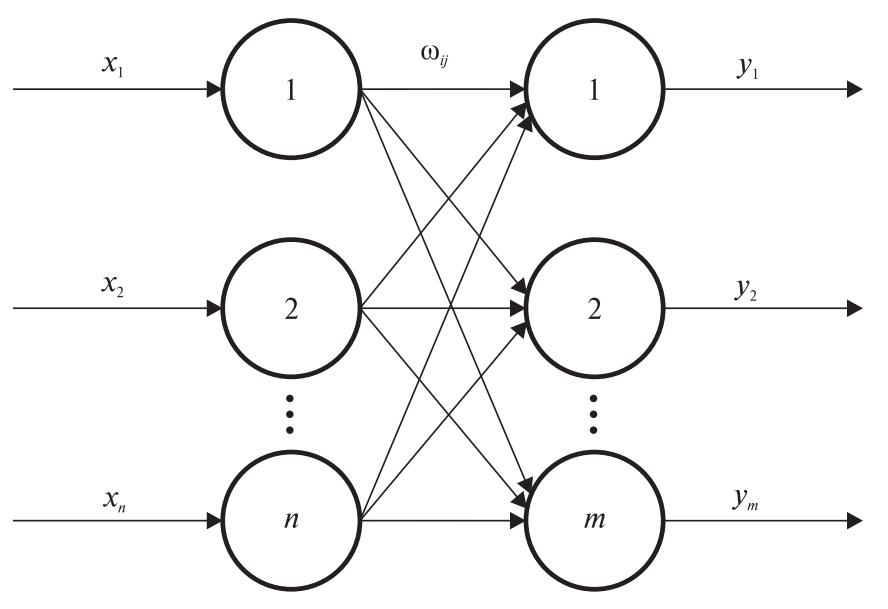
\includegraphics[width=0.4\linewidth]{figures/sd_ps/sd_ann/neural_network.png}}
	}

    \scnrelfrom{разбиение}{\scnkeyword{Типология и.н.с. по признаку направленности связей\scnsupergroupsign}}
    \scnaddlevel{1}
        \scneqtoset{
        искусственная нейронная сеть с прямыми связями\\
        \scnaddlevel{1}
            \scnsubdividing{
                персептрон\\
                \scnaddlevel{1}
                    \scnsubdividing{
                        персептрон Розенблатта;
                        автоэнкодерная искусственная нейронная сеть
                    }
                \scnaddlevel{-1}
                ;машина опорных векторов
                ;искусственная нейронная сеть радиально-базисных функций
            }
        \scnaddlevel{-1}
        ;искусственная нейронная сеть с обратными связями\\
        \scnaddlevel{1}
            \scnsubdividing{
                нейронная сеть Хопфилда
                ;нейронная сеть Хэмминга
            }
        \scnaddlevel{-1}
        ;рекуррентная искусственная нейронная сеть\\
        \scnaddlevel{1}
            \scnsubdividing{
            искусственная нейронная сеть Джордана
            ;искусственная нейронная сеть Элмана
            ;мультирекуррентная нейронная сеть
            ;LSTM-элемент
            ;GRU-элемент
            }
        \scnaddlevel{-1}
        }
    \scnaddlevel{-1}

    \scnrelfrom{разбиение}{\scnkeyword{Типология и.н.с. по признаку полноты связей\scnsupergroupsign}}
    \scnaddlevel{1}
        \scneqtoset{
        полносвязная искусственная нейронная сеть\\
        ;слабосвязная искусственная нейронная сеть
        }
    \scnaddlevel{-1}

    \scnrelfrom{решаемые задачи}{задачи, которые могут быть решены с помощью и.н.с. с приемлемой точностью}{
    \scnaddlevel{1}
    \scneqtoset{
        задача классификации\\
        \scnaddlevel{1}
            \scnsubset{задача}
            \scnexplanation{Задача построения классификатора, т.е. отображения $\tilde c: X \rightarrow C$, где $ X \in \mathbb{R}^m$ --
            признаковое пространство п.в.а., $C = {C_1, C_2, ...C_k }$ -- конечное и обычно небольшое множество меток классов.}
        \scnaddlevel{-1}
        ;задача регрессии\\
        \scnaddlevel{1}
            \scnsubset{задача}
            \scnexplanation{Задача построения оценочной функции по примерам $(x_i, f(x_i))$, где $f(x)$ -- неизвестная функция}
            \scnexplanation{\textbf{\textit{оценочная функция}} -- отображение вида $\tilde{f}: X \rightarrow \mathbb{R}$, где $X \in \mathbb{R}^m$ -- признаковое пространство п.в.а.}
        \scnaddlevel{-1}
        ;задача кластеризация\\
        \scnaddlevel{1}
            \scnsubset{задача}
            \scnexplanation{Задача разбиения множества п.в.а. на группы (кластеры) по какой-либо метрике сходства.}
        \scnaddlevel{-1}
        ;задача понижения размерности\\
        \scnaddlevel{1}
            \scnsubset{задача}
            \scnidtf{задача уменьшения размерности признакового пространства}
        \scnaddlevel{-1}
        ;задача управления\\
        \scnaddlevel{1}
            \scnsubset{задача}
        \scnaddlevel{-1}
        ;задача фильтрации\\
        \scnaddlevel{1}
            \scnsubset{задача}
        \scnaddlevel{-1}
        ;задача детекции\\
        \scnaddlevel{1}
            \scnsubset{задача}
            \scnsubset{задача классификации}
            \scnsubset{задача регрессии}
        \scnaddlevel{-1}
        ;задача с ассоциативной памятью\\
        \scnaddlevel{1}
            \scnsubset{задача}
        \scnaddlevel{-1}
    }
    }

\scnheader{формальный нейрон}
    \scnidtf{искусственный нейрон}
    \scnidtf{нейрон}
    \scnidtf{ф.н.}
    \scnidtf{нейронный элемент}
    \scnidtf{множество нейронов искусственных нейронных сетей}
    \scnidtf{математическая модель реального биологического нейрона}
    \scnnote{Отдельный формальный нейрон является искусственной нейронной сети с одним нейроном в единственном слое.}
    \scnsubset{искусственная нейронная сеть}
    \scnexplanation{\textbf{\textit{формальный нейрон}} -- это основной элемент \textit{искусственной нейронной сети}, применяющий свою \textit{функцию активации} (\scncite{Golovko2017}) к сумме произведений входных сигналов на весовые коэффициенты:
        \begin{equation*}
            y = F\left(\sum_{i=1}^{n} w_ix_i - T\right) = F(WX - T)
        \end{equation*}
        где $X = (x_1,x_2,...,x_n)^{T}$ -- вектор входного сигнала; $W - (w_1,w_2,...,w_n)$ -- вектор весовых коэффициентов; \textit{T} -- пороговое значение;
        \textit{F} -- функция активации.
    }

    \scnrelfrom{изображение}{
        \scnfileimage{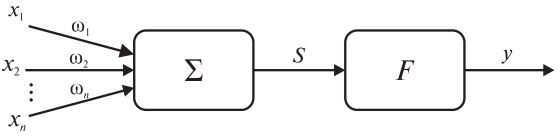
\includegraphics[width=0.4\linewidth]{figures/sd_ps/sd_ann/neuron.png}}
    }

    \scnnote{Формальные нейроны могут иметь полный набор связей с нейронами предшествующего слоя или неполный (разряженный)
        набор связей.}

    \scnsubdividing{
        полносвязный формальный нейрон\\
        \scnaddlevel{1}
            \scnidtf{нейрон, у которого есть полный набор связей с нейронами предшествующего слоя}
            \scnexplanation{отдельный обрабатывающий элемент и.н.с., выполняющий функциональное преобразование взвешенной суммы элементов вектора входных значений с помощью функции активации}
        \scnaddlevel{-1}
        ;сверточный формальный нейрон\\
        \scnaddlevel{1}
            \scnexplanation{Отдельный обрабатывающий элемент и.н.с., выполняющий функциональное преобразование результата
                операции свертки матрицы входных значений с помощью функции активации.}
            \scnnote{Сверточный формальный нейрон может быть представлен полносвязным формальным нейроном} 
            %\scnnote{Сверточный формальный нейрон с соответствующим ему ядром свертки может быть представлен нейроном с неполным набором связей.}
        \scnaddlevel{-1}
        ;рекуррентный формальный нейрон\\
        \scnaddlevel{1}
            \scnexplanation{Формальный нейрон, имеющий обратную связь с самим собой или с другими нейронами и.н.с.}
        \scnaddlevel{-1}
    }

\scnheader{формальный нейрон\scnrolesign}
    \scnidtf{формальный нейронный элемент\scnrolesign}
    \scnidtf{нейронный элемент\scnrolesign}
    \scnidtf{нейрон\scnrolesign}
    \scniselement{ролевое отношение}
    \scnrelfrom{первый домен}{искусственная нейронная сеть}
    \scnrelfrom{второй домен}{формальный нейрон}
    \scnrelfrom{область определения}{искусственная нейронная сеть}
    \scnexplanation{\textbf{\textit{формальный нейрон\scnrolesign}} -- ролевое отношение, связывающее искусственную нейронную сеть с ее нейроном.}

\scnheader{пороговый формальный нейрон\scnrolesign}
    \scnidtf{пороговый нейронный элемент\scnrolesign}
    \scnidtf{пороговый нейрон\scnrolesign}
    \scniselement{ролевое отношение}
    \scnrelfrom{первый домен}{искусственная нейронная сеть}
    \scnrelfrom{второй домен}{формальный нейрон}
    \scnrelfrom{область определения}{искусственная нейронная сеть}
    \scnexplanation{\textbf{\textit{пороговый формальный нейрон\scnrolesign}} -- ролевое отношение, связывающее искусственную нейронную сеть с таким ее нейроном,
            выходное значение которого всегда равно -1.
    }
    \scnexplanation{Весовой коэффициент синаптической связи, выходящей из такого нейрона, является порогом для нейрона, в который
        данная синаптическая связь входит.}

\scnheader{синаптическая связь}
    \scnidtf{синапс}
    \scnsubset{ориентированная пара}
    \scndefinition{\textbf{\textit{синаптическая связь}} -- ориентированная пара, первым компонентом которой является нейрон, из
        которого исходит сигнал, а вторым компонентом -- нейрон, который принимает этот сигнал.
    }

\scnheader{синаптическая связь\scnrolesign}
    \scnidtf{синапс\scnrolesign}
    \scniselement{ролевое отношение}
    \scnrelfrom{первый домен}{искусственная нейронная сеть}
    \scnrelfrom{второй домен}{синаптическая связь}
    \scnrelfrom{область определения}{\scnstartsetlocal\scnendstructlocal\\
        \scnreltoset{объединение}{искусственная нейронная сеть;синапс}
    }
    \scndefinition{\textbf{\textit{синаптическая связь\scnrolesign}} -- ролевое отношение, связывающее искусственную нейронную сеть с ее синапсом.
    }

\scnheader{параметр и.н.с.}
    \scnsubset{параметр}
    \scnsubdividing{
        настраиваемый параметр и.н.с.\\
        \scnaddlevel{1}
            \scnidtf{параметр и.н.с., значение которого изменяется в ходе обучения}
            \scnsubdividing{
                весовой коэффициент синаптической связи;
                пороговое значение;
                ядро свертки
                \scnaddlevel{1}
                    \scnidtf{квадратная матрица произвольного порядка, элементы которой изменяются в процессе
                        обучения и.н.с.}
                    \scnnote{если сверточный формальный нейрон представить в виде полносвязного формального нейрона, соответствующее ядро свертки преобразуется в вектор весовых коэффициентов}
                \scnaddlevel{-1}
            }
        \scnaddlevel{-1}\\
        ;архитектурный параметр и.н.с.\\
        \scnaddlevel{1}
            \scnnote{Параметр и.н.с., определяющий ее архитектуру.}
            \scnsubdividing{количество слоев;количество нейронов; количество синапсов}
        \scnaddlevel{-1}
    }

\scnheader{весовой коэффициент синаптической связи}
    \scnidtf{вес синапса}
    \scnidtf{сила синаптической связи}
    \scnsubset{настраиваемый параметр}
    \scnexplanation{\textbf{\textit{весовой коэффициент синаптической связи}} -- это числовой коэффициент, который ставится в соответствие каждому
        синапсу нейронной сети и изменяется в процессе обучения.
    }
    \scnnote{Если сила синаптической связи отрицательна, то она называется \textit{тормозящей}. В противном случае она
        является \textit{усиливающей}.
    }

\scnheader{входное значение формального нейрона*}
    \scnidtf{входное значение нейрона*}
    \scnidtf{входное значение*}
    \scniselement{неролевое отношение}
    \scniselement{бинарное отношение}
    \scnrelfrom{первый домен}{формальный нейрон}
    \scnrelfrom{второй домен}{число}
    \scnrelfrom{область определения}{\scnstartsetlocal\scnendstructlocal\\
        \scnreltoset{объединение}{формальный нейрон;число}
    }
    \scnexplanation{\textbf{\textit{входное значение формального нейрона*}} -- неролевое отношение, связывающее нейрон входного слоя со
        значением признака п.в.а., который подается на вход нейронной сети.
    }
    \scntext{теоретическая неточность}{Использование множества как формы представления входных данных является серьезным допущением, так как на практике
        входные данные структурированы более сложно -- в многомерные массивы. Самым близким теоретическим аналогом
        здесь выступает тензор. К сожалению, описание теории нейронных сетей с помощью тензорного исчисления в литературе
        как таковое отсутствует, но активно используется на практике: например, во многих разрабатываемых нейросетевых фреймворках.
        Формализация нейронных сетей с помощью тензоров видится авторам наиболее вероятным направлением работы в
        ближайших изданиях \textit{стандарта OSTIS}.
    }

\scnheader{паттерн входной активности и.н.с.}
	\scnidtf{п.в.а.}
    \scniselement{мультимножество}
    \scniselement{кортеж}
    \scnexplanation{\textbf{\textit{паттерн входной активности и.н.с.}} -- ориентированное мультимножество численных значений
        признаков некоторого объекта, которые могут выступать в качестве входных значений нейронов.
    }
	\scnnote{В текущей версии \textit{Стандарта OSTIS} предполагается, что п.в.а. содержит только предобработанные данные,
        то есть данные приведенные к численному виду и, возможно, преобразованные с помощью известных статистических
        методов (например, нормирования).
    }

\scnheader{признак}
    \scnidtf{feature}
    \scnidtf{множество признаков}
    \scnsubset{ролевое отношение}
    \scnexplanation{\textbf{\textit{признак}} -- множество ролевых отношений, каждое из которых связывает некоторый п.в.а. с численным значением, которое характеризует данный п.в.а. с какой-либо стороны.
    }

\scnheader{функция активации*}
    \scnidtf{функция активации нейрона*}
    \scniselement{неролевое отношение}
    \scniselement{бинарное отношение}
    \scnexplanation{\textbf{\textit{функция активации*}} -- неролевое отношение, связывающее формальный нейрон с функцией, результат
        применения которой к \textbf{\textit{взвешенной сумме нейрона}} определяет его \textbf{\textit{выходное значение}}.
    }
    \scnrelfrom{область определения}{\scnstartsetlocal\scnendstructlocal\\
        \scnreltoset{объединение}{формальный нейрон;функция}
    }
    \scnrelfrom{первый домен}{формальный нейрон}
    \scnrelfrom{второй домен}{функция}
    \scnaddlevel{1}
    \scnsubdividing{
        линейная функция\\
        \scnaddlevel{1}
            \scntext{формула}{
                \begin{equation*}
                    y = kS
                \end{equation*}
                где \textit{k} -- коэффициент наклона прямой, \textit{S} -- в.с.
            }
        \scnaddlevel{-1}
        ;пороговая функция\\
        \scnaddlevel{1}
            \scntext{формула}{
                \begin{equation*}
                    y = sign(S) =
                    \begin{cases}
                        1, S > 0,\\
                        0, S \leq 0
                    \end{cases}
                \end{equation*}
            }
        \scnaddlevel{-1}
        ;сигмоидная функция\\
        \scnaddlevel{1}
            \scntext{формула}{
                \begin{equation*}
                    y = \frac{1}{1+e^{-cS}}
                \end{equation*}
                где \textit{с} > 0 -- коэффициент, характеризующий ширину сигмоидной функции по оси абсцисс, \textit{S} -- в.с.
            }
        \scnaddlevel{-1}
        ;функция гиперболического тангенса\\
        \scnaddlevel{1}
            \scntext{формула}{
                \begin{equation*}
                    y = \frac{e^{cS}-e^{-cS}}{e^{cs}+e^{-cS}}
                \end{equation*}
                где \textit{с} > 0 -- коэффициент, характеризующий ширину сигмоидной функции по оси абсцисс, \textit{S} -- в.с.
            }
        \scnaddlevel{-1}
        ;функция softmax\\
        \scnaddlevel{1}
            \scntext{формула}{
                \begin{equation*}
                    y_j = softmax(S_j) = \frac{e^{S_j}}{\sum_{j} e^{S_j}}
                \end{equation*}
                где $S_j$ -- в.с. \textit{j}-го выходного нейрона
            }
        \scnaddlevel{-1}
        ;функция ReLU\\
        \scnaddlevel{1}
            \scntext{формула}{
                \begin{equation*}
                    y = F(S) =
                    \begin{cases}
                        S, S > 0,\\
                        kS, S \leq 0
                    \end{cases}
                \end{equation*}
                где \textit{k} = 0 или принимает небольшое значение, например, 0.01 или 0.001.
            }
        \scnaddlevel{-1}
    }
    \scnaddlevel{-1}

\scnheader{взвешенная сумма*}
    \scnidtf{взвешенная сумма входных значений*}
    \scnidtf{в.с.}
    \scniselement{неролевое отношение}
    \scniselement{бинарное отношение}
    \scnexplanation{\textbf{\textit{взвешенная сумма*}} -- неролевое отношение, связывающее формальный нейрон с числом, являющимся суммой
        произведений входных сигналов на весовые коэффициенты входящих в нейрон синаптических связей.
    }
    \scnrelfrom{область определения}{\scnstartsetlocal\scnendstructlocal\\
        \scnreltoset{объединение}{формальный нейрон;число}
    }
    \scnrelfrom{первый домен}{формальный нейрон}
    \scnrelfrom{второй домен}{число}
    \scnrelfrom{формула}{
        \begin{equation*}
            S = \sum_{i=1}^{n} w_ix_i - T
        \end{equation*}
        где \textit{n} -- размерность вектора входных значений, $w_i$ -- \textit{i}-тый элемент вектора весовых
        коэффициентов, $x_i$ -- \textit{i}-тый элемент вектора входных значений, \textit{T} -- пороговое значение.
    }

\scnheader{выходное значение формального нейрона*}
    \scnidtf{выходное значение нейрона*}
    \scnidtf{выходное значение*}
    \scniselement{неролевое отношение}
    \scniselement{бинарное отношение}
    \scnrelfrom{первый домен}{формальный нейрон}
    \scnrelfrom{второй домен}{число}
    \scnrelfrom{область определения}{\scnstartsetlocal\scnendstructlocal\\
        \scnreltoset{объединение}{формальный нейрон;число}
    }
    \scnexplanation{\textbf{\textit{входное значение*}} -- неролевое отношение, связывающее нейрон с числом, являющимся результатом применения
        функции активации нейрона к его взвешенной сумме.
    }
    \scnnote{Выходное значение нейрона является одним из входных сигналов для всех нейронов, в которые ведут выходящие из данного нейрона синапсы.
    }

\scnheader{слой и.н.с.}
    \scnidtf{слой}
    \scnidtf{слой искусственной нейронной сети}
    \scnidtf{множество слоев искусственных нейронных сетей}
    \scnnote{отдельный слой является искусственной нейронной сетью с одним слоем}
    \scnsubset{искусственная нейронная сеть}
    \scnexplanation{\textbf{\textit{слой и.н.с}}  -- это множество нейронных элементов, на которые в каждый такт времени
        параллельно поступает информация от других нейронных элементов сети (\scncite{Golovko2017})
    }
    \scnexplanation{\textbf{\textit{слой и.н.с.}} -- это множество формальных нейронов, осуществляющих параллельную независимую обработку
        вектора или матрицы входных значений
    }
    \scnnote{функция активации слоя является функцией активации всех формальных нейронов этого слоя}
    \scnnote{конфигурация слоя задается типом, количеством формальных нейронов, функцией активации}
    \scnnote{описание последовательности слоев и.н.с. с конфигурацией каждого слоя задает архитектуру и.н.с.}

    \scnsubdividing{
        полносвязный слой и.н.с.\\
        \scnaddlevel{1}
            \scnidtf{слой, в котором каждый нейрон имеет связь с каждым нейроном предшествующего слоя}
            \scnidtf{слой, в котором каждый нейрон является полносвязным}
        \scnaddlevel{-1}
        ;сверточный слой и.н.с.\\
        \scnaddlevel{1}
            \scnidtf{слой, в котором каждый нейрон является сверточным}
        \scnaddlevel{-1}
        ;слой и.н.с. нелинейного преобразования\\
        \scnaddlevel{1}
            \scnidtf{слой, осуществляющий нелинейное преобразование входных данных}
            \scnexplanation{Как правило, выделяются в отдельные слои только в программных реализациях. Фактически
                рассматриваются как финальный этап расчета выходной активности любого нейрона -- применение функции
                активации.}
            \scnnote{не изменяет размерность входных данных}
        \scnaddlevel{-1}
        ;dropout слой и.н.с.\\
        \scnaddlevel{1}
            \scnidtf{слой, реализующий технику регуляризации dropout}
            \scnnote{Данный тип слоя функционирует только во время обучения и.н.с.}
            \scnexplanation{Поскольку полносвязные слои имеют большое количество настраиваемых параметров, они
                подвержены эффекту переобучения. Один из способов устранить такой негативный эффект -- выполнить
                частичный отсев результатов на выходе полносвязного слоя. На этапе обучения техника dropout позволяет
                отбросить выходную активность некоторых нейронов с определенной, заданной вероятностью. Выходная
                активность ``отброшенных'' нейронов полагается равной нулю.}
        \scnaddlevel{-1}
        ;pooling слой и.н.с.\\
        \scnaddlevel{1}
            \scnidtf{подвыборочный слой}
            \scnidtf{объединяющий слой}
            \scnidtf{слой, осуществляющий уменьшение размерности входных данных}
        \scnaddlevel{-1}
        ;слой и.н.с. батч-нормализации\\
    }

\scnheader{распределяющий слой*}
    \scnidtf{входной слой*}
    \scniselement{неролевое отношение}
    \scniselement{бинарное отношение}
    \scndefinition{\textbf{\textit{распределяющий слой*}} -- неролевое отношение, связывающее искусственную нейронную сеть с ее слоем,
        нейроны которого принимают входные значения всей нейронной сети.
    }
    \scnrelfrom{область определения}{искусственная нейронная сеть}
    \scnrelfrom{первый домен}{искусственная нейронная сеть}
    \scnrelfrom{второй домен}{слой и.н.с.}

\scnheader{обрабатывающий слой*}
    \scniselement{неролевое отношение}
    \scniselement{бинарное отношение}
    \scndefinition{\textbf{\textit{обрабатывающий слой*}} -- неролевое отношение, связывающее искусственную нейронную сеть с ее слоем,
        нейроны которого принимают на вход выходные значения нейронов предыдущего слоя.
    }
    \scnrelfrom{область определения}{искусственная нейронная сеть}
    \scnrelfrom{первый домен}{искусственная нейронная сеть}
    \scnrelfrom{второй домен}{слой и.н.с}

\scnheader{выходной слой*}
    \scniselement{неролевое отношение}
    \scniselement{бинарное отношение}
    \scnexplanation{\textbf{\textit{выходной слой*}} -- неролевое отношение, связывающее искусственную нейронную сеть с ее слоем,
        выходные значения нейронов которого являются выходными значениями всей нейронной сети.
    }
    \scnrelfrom{область определения}{искусственная нейронная сеть}
    \scnrelfrom{первый домен}{искусственная нейронная сеть}
    \scnrelfrom{второй домен}{слой и.н.с}

\bigskip
\scnendstruct \scnendsegmentcomment{Предметная область и онтология искусственных нейронных сетей}

\scnsegmentheader{Предметная область и онтология действий по обработке искусственной нейронной сети}
\scnstartsubstruct

\newpage
\scnheader{Предметная область действий по обработке искусственных нейронных сетей}
    \scnidtf{Предметная область действий по обработке и.н.с.}
    \scniselement{предметная область}
    \scnsdmainclass{действие по обработке искусственных нейронных сетей}
    \scnsdclass{
        действие по обработке искусственных нейронных сетей;
        действие конфигурации весовых коэффициентов и.н.с.;
        действие конфигурации и.н.с.;
        действие интерпретации и.н.с.;
        метод обучения и.н.с.;
        метод обучения с учителем;
        метод обратного распространения ошибки;
        метод обучения без учителя;
        метод оптимизации;
        функция потерь;
        параметр обучения;
        скорость обучения;
        моментный параметр;
        параметр регуляризации;
        размер группы обучения;
        количество эпох обучения;
        выборка
    }
    \scnsdrelation{
        обучающая выборка\scnrolesign;
        тестовая выборка\scnrolesign;
        валидационная выборка\scnrolesign;
        метод обучения\scnrolesign;
        метод оптимизации\scnrolesign;
        функция потерь\scnrolesign
    }

\scnheader{действие по обработке искусственной нейронной сети}
    \scnidtf{действие по обработке и.н.с.}
    \scnidtf{действие с искусственной нейронной сетью}
    \scnsubset{действие}
    \scnexplanation{В зависимости от того, является ли искусственная нейронная сеть знаком внешней по отношению к памяти системы сущности,
        элементы множества действие по обработке и.н.с. являются либо элементами множества \textbf{\textit{действие, выполняемое кибернетической
        системой в своей внешней среде}}, либо элементом множества \textbf{\textit{действие, выполняемое кибернетической системой
        в собственной памяти.
    }}.
    }
    \scnsubdividing{
        действие конфигурации и.н.с.\\
        \scnaddlevel{1}
        \scnsubdividing{
            действие создания и.н.с.
            ;действие редактирования и.н.с.
            ;действие удаления и.н.с.
            ;действие конфигурации слоя и.н.с.\\
            \scnaddlevel{1}
                \scnsubdividing{
                    действие добавления слоя в и.н.с.
                    ;действие редактирования слоя и.н.с.
                    ;действие удаления слоя и.н.с.
                    ;действие установки функции активации нейронов слоя и.н.с.
                    ;действие конфигурации нейрона в слое и.н.с\\
                    \scnaddlevel{1}
                        \scnsubdividing{
                            действие добавления нейрона в слой и.н.с.
                            ;действие редактирования нейрона в слое и.н.с.
                            ;действие удаления нейрона из слоя и.н.с.
                            ;действие установки функции активации нейрона в слое и.н.с.
                        }
                    \scnaddlevel{-1}
                }
            \scnaddlevel{-1}
        }
        \scnaddlevel{-1}
        ;действие конфигурации весовых коэффициентов и.н.с.\\
        \scnaddlevel{1}
            \scnsuperset{действие обучения и.н.с.}
            \scnsuperset{действие начальной инициализации весов и.н.с.}
            \scnaddlevel{1}
                \scnsuperset{действие начальной инициализации весов нейронов слоя и.н.с.}
                \scnaddlevel{1}
                    \scnsuperset{действие начальной инициализации весов нейрона и.н.с.}
                \scnaddlevel{-1}
            \scnaddlevel{-1}
        \scnaddlevel{-1}
        ;действие интерпретации и.н.с.
    }
    \scnnote{Действия по обработке и.н.с осуществляет соответствующий коллектив агентов.}
    \scnexplanation{Так как в результате действий по обработке и.н.с объект этих действий, конкретная и.н.с, может существенно меняться
        (меняется конфигурация сети, ее весовые коэффициенты), то и.н.с представляется в базе знаний как темпоральное объединение
        всех ее версий. Каждая версия является и.н.с. и темпоральной сущностью. На множестве этих темпоральных сущностей задается
        темпоральная последовательность с указанием первой и последней версии. Для каждой версии описываются специфичные знания.
        Общие для всех версий знания описываются для и.н.с, являющейся темпоральным объединением всех версий.
    }
    \scnaddlevel{1}
        \scnrelfrom{пример}{
            \scnfilescg{figures/sd_ps/sd_ann/temporal_neural_network_scg.png}
        }
    \scnaddlevel{-1}

\scnheader{действие обучения и.н.с.}
    \scnidtf{действие обучения искусственной нейронной сети}
    \scnsubset{действие конфигурации весовых коэффициентов и.н.с.}
    \scndefinition{\textbf{\textit{действие обучения и.н.с.}} -- действие, в ходе которого реализуется определенный метод обучения
        и.н.с. с заданными параметрами обучения и.н.с, методом оптимизации и функцией потерь.
    }
    \scnrelfromset{известные проблемы}{
        \scnfileitem{Переобучение -- проблема, возникающая при обучении и.н.с., заключающаяся в том,
        что сеть хорошо адаптируется к п.в.а. из обучающей выборки, при этом теряя способность к обобщению.
        Переобучение возникает из-за применения неоправданно сложной модели при обучении и.н.с. Это происходит,
        когда количество настраиваемых параметров и.н.с. намного больше размера обучающей выборки. Возможные
        варианты решения проблемы заключаются в упрощении модели, увеличении выборки, использовании регуляризации
        (параметр регуляризации, техника dropout и т.д.).\\
        Обнаружение переобученности сложнее, чем недообученности. Как правило, для этого применяется
        кросс-валидация на валидационной выборке, позволяющая оценить момент завершения процесса обучения.
        Идеальным вариантом является достижение баланса между переобученностью и недообученностью.
        };
        \scnfileitem{Недообучение -- проблема, возникающая при обучении и.н.с., заключающаяся в том,
        что сеть дает одинаково плохие результаты на обучающей и контрольной выборках.
        Чаще всего такого рода проблема возникает при недостаточном времени, затраченном на обучение модели.
        Однако это может быть вызвано и слишком простой архитектурой модели либо малым размером обучающей
        выборки. Соответственно решение, которое может быть принято ML-инженером, заключается в устранении
        этих недостатков: увеличение времени обучения, использование модели с большим числом настраиваемых
        параметров, увеличение размера обучающей выборки, а также уменьшение регуляризации и более тщательный
        отбор признаков для обучающих примеров.
        }
    }
    \scnrelfrom{описание примера}{
        \scnfilescg{figures/sd_ps/sd_ann/ann_trainning_scg.png}
    }

\scnheader{выборка}
    \scnsubset{множество}
	\scnexplanation{\textbf{\textit{выборка}} -- множество п.в.а., используемых в процессе обучения, тестирования
        и архитектурной настройки и.н.с.
    }

\scnheader{обучающая выборка\scnrolesign}
    \scnidtf{training set\scnrolesign}
    \scniselement{ролевое отношение}
    \scnrelfrom{первый домен}{действие обучения и.н.с.}
    \scnrelfrom{второй домен}{выборка}
    \scnrelfrom{область определения}{\scnstartsetlocal\scnendstructlocal\\
        \scnreltoset{объединение}{действие обучения и.н.с.;выборка}
    }
    \scnexplanation{\textbf{\textit{обучающая выборка\scnrolesign}} -- ролевое отношение, связывающее действие обучения и.н.с. с выборкой,
        используемой для изменения настраиваемых параметров и.н.с. в процессе ее обучения.
    }

\scnheader{тестовая выборка\scnrolesign}
    \scnidtf{test set\scnrolesign}
    \scniselement{ролевое отношение}
    \scnrelfrom{первый домен}{действие обучения и.н.с.}
    \scnrelfrom{второй домен}{выборка}
    \scnrelfrom{область определения}{\scnstartsetlocal\scnendstructlocal\\
        \scnreltoset{объединение}{действие обучения и.н.с.;выборка}
    }
    \scnexplanation{\textbf{\textit{тестовая выборка\scnrolesign}} -- ролевое отношение, связывающее действие обучения и.н.с. с выборкой,
        используемой для проверки обобщающей способности обученной и.н.с.
    }
    \scnnote{Элементы контрольной выборки не используются в процессе обучения.}
\right) 
\scnheader{валидационная выборка\scnrolesign}
    \scniselement{ролевое отношение}
    \scnrelfrom{первый домен}{действие обучения и.н.с.}
    \scnrelfrom{второй домен}{выборка}
    \scnrelfrom{область определения}{\scnstartsetlocal\scnendstructlocal\\
        \scnreltoset{объединение}{действие обучения и.н.с.;выборка}
    }
    \scnexplanation{\textbf{\textit{валидационная выборка\scnrolesign}} -- ролевое отношение, связывающее действие обучения и.н.с. с выборкой,
        используемой для определения (настройки) архитектурных параметров и.н.с. и параметров обучения.
    }
    \scnnote{Элементы валидационной выборки не используются в процессе обучения (не входят в обучающую выборку).}


\scnheader{метод обучения и.н.с.}
    \scnsubset{метод}
	\scnexplanation{\textbf{\textit{метод обучения и.н.с.}} -- метод итеративного поиска оптимальных значений настраиваемых параметров и.н.с.,
        минимизирующих некоторую заданную функцию потерь.
    }
	\scnnote{Стоит отметить, что хотя целью применения метода обучения является минимизация функции потерь, ``полезность''
        полученной после обучения модели можно оценить только по достигнутому уровню ее обобщающей способности.
    }
	\scnsuperset{метод обучения с учителем}
	\scnaddlevel{1}
		\scnexplanation{
            \textbf{\textit{метод обучения с учителем}} -- метод обучения с использованием заданных целевых переменных.
        }
		\scnsuperset{метод обратного распространения ошибки}
		\scnaddlevel{1}
			\scnidtf{м.о.р.о.}
			\scntext{алгоритм}{\\
				\begin{minipage}{\linewidth}
					\vspace{-\baselineskip}
					\begin{algorithm}[H]
						\KwData{$X$ -- данные, $Et$ -- желаемый отклик (метки), $E_m$ -- желаемая ошибка (в соответствии с выбранной функцией потерь)}
						\KwResult{обученная нейронная сеть \textit{Net}}
						инициализация весов \textit{W} и порогов \textit{T};\\
						\Repeat{$E<E_m$}{
							\ForEach{$x \in X$ \And $e \in Et$}{
								фаза прямого распространения сигнала: вычисляются активации для всех слоев и.н.с.;\\
								фаза обратного распространения ошибки: вычисляются ошибки для последнего слоя и всех предшествующих слоев;\\
								изменение настраиваемых параметров и.н.с. в соответствии с вычисленными ошибками;\\
							}
							вычисление общей ошибки E на данной эпохе;
						}
					\end{algorithm}
				\end{minipage}
            }
			\scnnote{м.о.р.о. использует заданный метод оптимизации и заданную функцию потерь для реализации фазы
                обратного распространения ошибки и изменения настраиваемых параметров и.н.с. Одним из самых распространенных
                методов оптимизации является метод стохастического градиентного спуска. Приведенный м.о.р.о. используется
                для реализации последовательного варианта обучения.
            }
			\scnnote{Следует также отметить, что несмотря на то, что метод отнесен к методам обучения с учителем, в случае
                использования м.о.р.о. для обучения автокодировщиков в классических публикациях он рассматривается как
                метод обучения без учителя, поскольку в данном случае размеченные данные отсутствуют.
            }
		\scnaddlevel{-1}
	\scnaddlevel{-1}
	\scnsuperset{метод обучения без учителя}
	\scnaddlevel{1}
		\scnexplanation{\textbf{\textit{метод обучения без учителя}} -- метод обучения без использования заданных целевых переменных
            (в режиме самоорганизации)
        }
		\scnexplanation{В ходе выполнения алгоритма метода обучения без учителя выявляются полезные структурные свойства
            набора. Неформально его понимают как метод для извлечения информации из распределения, выборка для которого
            не была вручную аннотирована человеком (\scncite{Goodfellow2017}).
        }
	\scnaddlevel{-1}

\scnheader{метод обучения\scnrolesign}
    \scniselement{ролевое отношение}
    \scnrelfrom{первый домен}{действие обучения и.н.с.}
    \scnrelfrom{второй домен}{метод обучения и.н.с.}
    \scnrelfrom{область определения}{\scnstartsetlocal\scnendstructlocal\\
        \scnreltoset{объединение}{действие обучения и.н.с.;метод обучения и.н.с.}
    }
    \scnexplanation{\textbf{\textit{метод обучения\scnrolesign}} -- ролевое отношение, связывающее действие обучения и.н.с. с методом обучения,
        использующимся для обучения и.н.с. в рамках этого действия.
    }

\newpage
\scnheader{метод оптимизации}
    \scnsubset{метод}
	\scndefinition{\textbf{\textit{метод оптимизации}} -- метод для минимизации целевой функции потерь при обучении и.н.с.}
	\scnrelfromlist{включение}{
		SGD\\
		\scnaddlevel{1}
			\scnidtf{стохастический градиентный спуск}
			\scnidtf{с.г.с.}
			\scnidtf{stochastic gradient descent}
			\scnnote{В методе стохастического градиентного спуска корректировка настраиваемых параметров и.н.с. выполняется в направлении максимального уменьшения функции стоимости, т.е. в направлении, противоположном вектору градиента функции потерь (\scncite{Haykin2006})}
		\scnaddlevel{-1}
		;Nesterov method\\
		\scnaddlevel{1}
			\scnidtf{метод Нестерова}
			\scnnote{Обучение методом с.г.с. иногда происходит очень медленно. Импульсный метод позволяет ускорить обучение, особенно в условиях высокой кривизны, небольших, но устойчивых градиентов или зашумленных градиентов. В импульсном методе вычисляется экспоненциально затухающее скользящее среднее прошлых градиентов и продолжается движение в этом направлении. Метод Нестерова является вариантом импульсного алгоритма, в котором градиент вычисляется после применения текущей скорости (\scncite{Goodfellow2017})}
		\scnaddlevel{-1}
		;AdaGrad\\
		\scnaddlevel{1}
			\scnidtf{adaptive gradient}
			\scnnote{Данный метод по отдельности адаптирует скорости обучения всех настраиваемых параметров и.н.с., умножая их на коэффициент, обратно пропорциональный квадратному корню из суммы всех прошлых значений квадрата градиента (\scncite{Duchi2011})}
		\scnaddlevel{-1}
		;RMSProp\\
		\scnaddlevel{1}
			\scnidtf{root mean square propagation}
			\scnnote{Данный метод является модификацией AdaGrad, которая позволяет улучшить его поведение в невыпуклом случае путем изменения способа агрегирования градиента на экспоненциально взвешенное скользящее среднее. Использование экспоненциально взвешенного скользящего среднего гарантирует повышение скорости сходимости после обнаружения выпуклой впадины, как если бы внутри этой впадины алгоритм AdaGrad был инициализирован заново (\scncite{Goodfellow2017})}
		\scnaddlevel{-1}	
		;Adam\\
		\scnaddlevel{1}
			\scnidtf{adaptive moments}
			\scnnote{Данный метод можно рассматривать как комбинацию RMSProp и AdaGrad (\scncite{Kingma2014}). Помимо усредненного первого момента, данный метод использует усредненное значение вторых моментов градиентов}
		\scnaddlevel{-1}
	}
	\scnnote{Успешность применения методов оптимизации зависит главным образом от знакомства пользователя с соответствующим
        алгоритмом (\scncite{Goodfellow2017}).
    }

\scnheader{метод оптимизации\scnrolesign}
    \scniselement{ролевое отношение}
    \scnrelfrom{первый домен}{метод обучения и.н.с.}
    \scnrelfrom{второй домен}{метод оптимизации}
    \scnrelfrom{область определения}{\scnstartsetlocal\scnendstructlocal\\
        \scnreltoset{объединение}{метод обучения и.н.с.;метод оптимизации}
    }
    \scnexplanation{\textbf{\textit{метод оптимизации\scnrolesign}} -- ролевое отношение, связывающее метод обучения и.н.с. с методом оптимизации,
        использующимся для обучения и.н.с. с помощью данного метода.
    }

\scnheader{функция потерь}
    \scnsubset{функция}
	\scnexplanation{\textbf{\textit{функция потерь}} -- функция, используемая для вычисления ошибки, рассчитываемой как разница между фактическим
        эталонным значением и прогнозируемым значением, получаемым и.н.с.
    }
    \scnrelfromlist{включение}{
		MSE\\
		\scnaddlevel{1}
			\scnidtf{mean square error}
			\scnidtf{средняя квадратичная ошибка}
			\scntext{формула}{
				\begin{equation*}
					MSE = \frac{1}{L} \sum_{l=1}^L \sum_{i=1}^m (y_i^l - e_i^l)^2
				\end{equation*}
				где $y_i^l$ -- прогноз модели, $e_i^l$ -- ожидаемый (эталонный) результат, \textit{m} -- размерность выходного вектора, \textit{L} -- объем обучающей выборки.
			}
		\scnaddlevel{-1}
		;BCE\\
		\scnaddlevel{1}
			\scnidtf{binary cross entropy}
			\scnidtf{бинарная кросс-энтропия}
			\scntext{формула}{
				\begin{equation*}
					BCE = - \sum_{l=1}^L (e^l \log(y^l) + (1 - e^l)\log(1 - y^l))
				\end{equation*}
				где $y^l$ -- прогноз модели, $e^l$ -- ожидаемый (эталонный) результат: \textit{0} или \textit{1}, \textit{L} -- объем обучающей выборки.
			}
			\scnnote{для бинарной кросс-энтропии в выходном слое и.н.с. будет находиться один нейрон}
		\scnaddlevel{-1}
		;MCE\\
		\scnaddlevel{1}
			\scnidtf{multi-class cross entropy}
			\scnidtf{мультиклассовая кросс-энтропия}
			\scntext{формула}{
				\begin{equation*}
					MCE = - \sum_{l=1}^L \sum_{i=1}^m e_{i}^l \log(y_{i}^l)
				\end{equation*}
				где $y_{i}^l$ -- прогноз модели, $e_i^l$ -- ожидаемый (эталонный результат), \textit{m} -- размерность выходного вектора
			}
			\scnnote{для мультиклассовой кросс-энтропии количество нейронов в выходном слое и.н.с. совпадает с количеством классов}
		\scnaddlevel{-1}
	}
	\scnnote{Для решения задачи классификации рекомендуется использовать бинарную или мультиклассовую кросс-энтропийную функцию потерь,
        для решения задачи регрессии рекомендуется использовать среднюю квадратичную ошибку.
    }

\scnheader{функция потерь\scnrolesign}
    \scniselement{ролевое отношение}
    \scnrelfrom{первый домен}{метод обучения и.н.с.}
    \scnrelfrom{второй домен}{функция потерь}
    \scnrelfrom{область определения}{\scnstartsetlocal\scnendstructlocal\\
        \scnreltoset{объединение}{метод обучения и.н.с.;функция потерь}
    }
    \scnexplanation{\textbf{\textit{функция потерь\scnrolesign}} -- ролевое отношение, связывающее метод обучения и.н.с. с функцией потерь,
        использующимся для обучения и.н.с. с помощью данного метода.
    }

\scnheader{параметр обучения}
   \scnidtf{группа наиболее общих параметров метода обучения и.н.с.}
   \scnrelfromset{состав группы параметров обучения}{
       скорость обучения\\
          \scnaddlevel{1}
              \scnexplanation{\textbf{\textit{скорость обучения}} -- параметр, определяющий скорость изменения параметров и.н.с.
                в процессе обучения.
              }
          \scnaddlevel{-1}
       ;моментный параметр\\
          \scnaddlevel{1}
                \scnidtf{момент}
                \scnidtf{momentum}
                \scnexplanation{\textbf{\textit{моментный параметр}} -- параметр, используемый в процессе обучения для устранения
                    проблемы ``застревания'' алгоритма обучения в локальных минимумах минимизируемой функции потерь.
                }
                \scnexplanation{При обучении и.н.с. частой является ситуация остановки процесса в определенной точке локального
                    минимума без достижения желаемого уровня обобщающей способности и.н.с. Для устранения такого
                    нежелательного явления вводится дополнительный параметр (момент) позволяющий алгоритму обучения
                    ``перескочить'' через локальный минимум и продолжить процесс.
                }
         \scnaddlevel{-1}
       ;параметр регуляризации\\
         \scnaddlevel{1}
             \scnexplanation{\textbf{\textit{параметр регуляризации}} -- параметр, применяемый для контроля уровня переобучения и.н.с.
             }
             \scnexplanation{\textbf{\textit{регуляризация}} -- добавление дополнительных ограничений к правилам изменения настраиваемых
                параметров и.н.с. с целью предотвратить переобучение.
             }
         \scnaddlevel{-1}
       ;размер группы обучения\\
         \scnaddlevel{1}
             \scnexplanation{\textbf{\textit{размер группы обучения}} -- размер группы п.в.а., которая используется для изменения параметров
                и.н.с. на каждом элементарном шаге обучения.
             }
         \scnaddlevel{-1}
       ;количество эпох обучения\\
       \scnaddlevel{1}
       		\scnexplanation{\textbf{\textit{эпоха обучения}} -- одна итерация алгоритма обучения, в ходе которой все обучающие п.в.а.
                из обучающей выборки были однократно использованы.
            }
       \scnaddlevel{-1}
   }

\bigskip
\scnendstruct \scnendsegmentcomment{Предметная область и онтология действий по обработке искусственной нейронной сети}

\bigskip
\scnendstruct \scnendcurrentsectioncomment

\end{SCn}

\scsubsection{\textbf{Предметная область и онтология интерфейсов ostis-систем}}
\label{sec:sd_interfaces}

\scsubsubsection{Предметная область и онтология входящих в ostis-систему и выходящих из ostis-системы сообщений}
\scsubsubsection{Предметная область и онтология интерфейсных действий пользователей ostis-системы}
\scsubsubsection{Предметная область и онтология действий и внутренних агентов пользовательского интерфейса ostis-системы}
\scsubsubsection{Предметная область и онтология знаковых конструкций и языков}
\scsubsubsection{Предметная область и онтология естественных языков}
\begin{SCn}

\scnsectionheader{\currentname}

\scnstartsubstruct

\scnheader{Предметная область естественных языков}
\scniselement{предметная область}
\scnsdmainclasssingle{язык}
\scnsdclass{плановый язык;язык общения;лексема;номинативная единица;комбинаторный вариант лексемы;естественный язык;тайген;ёген}
\scnsdrelation{морфологическая парадигма*;член предложения\scnrolesign }

\scnheader{язык}
\scnsubdividing{естественный язык\\
	\scnaddlevel{1}
	\scnexplanation{Естественный язык представляет собой язык, который не был создан целенаправленно}
	\scnaddlevel{-1}
;искусственный язык\\
	\scnaddlevel{1}
	\scnexplanation{Искусственный язык представляет собой язык, специально разработанный для достижения определённых целей}
	\scnhaselement{Эсперанто}
	\scnhaselement{Python}
	\scnsuperset{сконструированный язык}
	\scnaddlevel{1}
	\scnexplanation{Сконструированный язык представляет собой искусственный язык, предназначенный для общения людей}
	\scnhaselement{Эсперанто}
	\scnaddlevel{-1}
	\scnaddlevel{-1}
}
\scnsuperset{международный язык}
	\scnaddlevel{1}
	\scnexplanation{Международный язык представляет собой естественный или искусственный язык, использующийся для общения людей разных из стран}
	\scnhaselement{Английский язык}
	\scnhaselement{Русский язык}
	\scnaddlevel{-1}

\scnheader{плановый язык}
\scnreltoset{пересечение}{сконструированный язык;международный язык}

\scnheader{язык общения}
\scnreltoset{объединение}{естественный язык;сконструированный язык}
\scnhaselement{Английский язык}
\scnhaselement{Русский язык}
\scnhaselement{Эсперанто}
\scnreltoset{объединение}{корневой язык\\
	\scnaddlevel{1}
	\scnexplanation{Корневой язык представляет собой язык, для которого характерно полное отсутствие словоизменения и наличие грамматической значимости порядка слов, состоящих только из корня.}
	\scnhaselement{Английский язык}
	\scnaddlevel{-1}
;агглютинативный язык\\
	\scnaddlevel{1}
	\scnexplanation{Агглютинативный язык характеризуется развитой системой употребления суффиксов, приставок, добавляемых к неизменяемой основе слова, которые используются для выражения категорий числа, падежа, рода и др.}
	\scnhaselement{Английский язык}
	\scnaddlevel{-1}
;флективный язык\\
	\scnaddlevel{1}
	\scnexplanation{Для флективного языка характерно развитое употребление окончаний для выражения категорий рода, числа, падежа, сложная система склонения глаголов, чередование гласных в корне, а также строгое различение частей речи.}
	\scnhaselement{Русский язык}
	\scnaddlevel{-1}
;профлективный язык\\
	\scnaddlevel{1}
	\scnexplanation{Для профлективного языка характерны агглютинация (в случае именного словоизменения), флексия и чередование гласных (аблаут)(в случае глагольного словоизменения).}
	\scnaddlevel{-1}
}

\scnheader{лексема}
\scnsubset{файл}
\scnexplanation{\textit{Лексема} -- тайген или ёген конкретного естественного языка.}
	\scnaddlevel{1}
	\scnrelfrom{источник}{\scncite{Hardzei2005}}
	\scnaddlevel{-1}
	
\scnheader{номинативная единица}
\scnsubset{файл}
\scnexplanation{\textit{Номинативная единица} -- устойчивая последовательность комбинáторных вариантов лексем, в которой один вариант лексемы (модификатор) определяет другой (актуализатор), например: ‘записная книжка’, ‘бежать галопом’.}
	\scnaddlevel{1}
	\scnrelfrom{источник}{\scncite{Hardzei2005}}
	\scnaddlevel{-1}
	
\scnheader{комбинаторный вариант лексемы}
\scnsubset{файл}
\scnexplanation{\textit{Комбинáторный вариант лексемы } -- вариант лексемы в упорядоченном наборе её вариантов (парадигме).}
	\scnaddlevel{1}
	\scnrelfrom{источник}{\scncite{Hardzei2007}}
	\scnaddlevel{-1}


\scnheader{морфологическая парадигма*}
\scniselement{квазибинарное отношение}
\scnexplanation{\textit{Морфологическая парадигма*} -- квазибинарное отношение, связывающее лексему с её комбинáторными вариантами.}
\scnrelfrom{первый домен}{словоформа}
\scnrelfrom{второй домен}{лексема}

\scnheader{естественный язык}
\scnsubdividing{
	часть языка\\
	\scnaddlevel{1}
	\scnsubdividing{тайген;ёген}
	\scnaddlevel{-1}
	;знак алфавита синтаксиса\\
		\scnaddlevel{1}
		\scnexplanation{\textit{Знаки алфавита синтаксиса} -- вспомогательные средства синтаксиса (на макроуровне -- предлоги, послелоги, союзы, частицы и др., на микроуровне -- флексии, префиксы, постфиксы, инфиксы и др.), служащие для соединения составных частей языковых структур и образования морфологических парадигм.}
			\scnaddlevel{1}
			\scnrelfrom{источник}{\scncite{Hardzei2005}}
			\scnaddlevel{-1}
		\scnaddlevel{-1}
}

\scnheader{тайген}
\scnexplanation{\textit{Тайген} -- часть языка, обозначающая индивида.}
	\scnaddlevel{1}
	\scnrelfrom{источник}{\scncite{Hardzei2006}}
	\scnrelfrom{источник}{\scncite{Hardzei2015}}
	\scnaddlevel{-1}
\scnsubdividing{
	развёрнутый тайген\\
	\scnaddlevel{1}
	\scnsubdividing{
		составной тайген\\
		;сложный тайген\\
	}   
	\scnaddlevel{-1}
	;свёрнутый тайген\\
	\scnaddlevel{1}
	\scnsubdividing{
		сокращённый тайген\\
		;сжатый тайген\\
			\scnaddlevel{1}
			\scnsubdividing{
				информационный тайген\\
				\scnaddlevel{1}
				\scnexplanation{\textit{Информационный тайген} -- тайген, обозначающий индивида в информационном фрагменте модели мира.}
					\scnaddlevel{1}
					\scnrelfrom{источник}{\scncite{Hardzei2006}}
					\scnrelfrom{источник}{\scncite{Hardzei2015}}
					\scnaddlevel{-1}
				\scnaddlevel{-1}
				;физический тайген\\
				\scnaddlevel{1}
				\scnexplanation{\textit{Физический тайген} -- тайген, обозначающий индивида в физическом фрагменте модели мира. }
					\scnaddlevel{1}
					\scnrelfrom{источник}{\scncite{Hardzei2006}}
					\scnrelfrom{источник}{\scncite{Hardzei2015}}
					\scnaddlevel{-1}
				\scnsubdividing{
					постоянный тайген\\
					\scnaddlevel{1}
					\scnexplanation{\textit{Постоянный тайген} -- физический тайген, обозначающий постоянного индивида.}
						\scnaddlevel{1}
						\scnrelfrom{источник}{\scncite{Hardzei2006}}
						\scnrelfrom{источник}{\scncite{Hardzei2015}}
						\scnaddlevel{-1}
					\scnaddlevel{-1}
					;переменный тайген\\
					\scnaddlevel{1}
					\scnexplanation{\textit{Переменный тайген} -- физический тайген, обозначающий переменного индивида.}
						\scnaddlevel{1}
						\scnrelfrom{источник}{\scncite{Hardzei2006}}
						\scnrelfrom{источник}{\scncite{Hardzei2015}}
						\scnaddlevel{-1}
					\scnaddlevel{-1}
				}
				\scnsubdividing{
					качественный тайген
					;количественный тайген\\
				}
				\scnsubdividing{
					одноместный тайген
					;многоместный тайген\\
					\scnaddlevel{1}
					\scnsuperset{интенсивный тайген}
					\scnsuperset{экстенсивный тайген}
					\scnaddlevel{-1}	
				}
			}
			\scnaddlevel{-1}
	}
	\scnaddlevel{-1}
}
\scnaddlevel{-1}	

\scnheader{ёген}
\scnexplanation{\textit{Ёген} -- часть языка, обозначающая признак индивида.}
	\scnaddlevel{1}
	\scnrelfrom{источник}{\scncite{Hardzei2006}}
	\scnrelfrom{источник}{\scncite{Hardzei2015}}
	\scnaddlevel{-1}
\scnsubdividing{
	развёрнутый ёген\\
	\scnaddlevel{1}
	\scnsubdividing{
		составной ёген
		;сложный ёген
	}
	\scnaddlevel{-1}
	;свёрнутый ёген\\
	\scnaddlevel{1}
	\scnsubdividing{
		сокращённый ёген\\
			\scnaddlevel{1}
			\scnsubdividing{
				информационный ёген\\
					\scnaddlevel{1}
					\scnexplanation{\textit{Информационный ёген} -- еген, обозначающий признак индивида в информационном фрагменте модели мира.}
						\scnaddlevel{1}
						\scnrelfrom{источник}{\scncite{Hardzei2006}}
						\scnrelfrom{источник}{\scncite{Hardzei2007a}}
						\scnaddlevel{-1}
					\scnaddlevel{-1}
				;физический ёген\\
				\scnaddlevel{1}
				\scnexplanation{\textit{Физический ёген} -- еген, обозначающий признак индивида в физическом фрагменте модели мира.}
					\scnaddlevel{1}
					\scnrelfrom{источник}{\scncite{Hardzei2006}}
					\scnrelfrom{источник}{\scncite{Hardzei2007a}}
					\scnaddlevel{-1}
				\scnsubdividing{
					постоянный ёген\\
						\scnaddlevel{1}
						\scnexplanation{\textit{Постоянный ёген} - физический ёген, обозначающий постоянный признак индивида.}
							\scnaddlevel{1}
							\scnrelfrom{источник}{\scncite{Hardzei2006}}
							\scnrelfrom{источник}{\scncite{Hardzei2007a}}
							\scnaddlevel{-1}
						\scnaddlevel{-1}
					;переменный ёген\\
						\scnaddlevel{1}
						\scnexplanation{\textit{Переменный ёген} -- физический ёген, обозначающий переменный признак индивида.}
							\scnaddlevel{1}
							\scnrelfrom{источник}{\scncite{Hardzei2006}}
							\scnrelfrom{источник}{\scncite{Hardzei2007a}}
							\scnaddlevel{-1}
						\scnaddlevel{-1}
				}
				\scnsubdividing{
					качественный ёген
					;количественный ёген
				}
				\scnsubdividing{
					одноместный ёген
					;многоместный ёген\\
						\scnaddlevel{1}
						\scnsubdividing{
							интенсивный ёген
							;экстенсивный ёген
						}
						\scnaddlevel{-1}
				}
				\scnaddlevel{-1}
			}
			\scnaddlevel{-1}
		;сжатый ёген
	}
	\scnaddlevel{-1}
}

\scnheader{Пример sc.g-текста, описывающего лексему}
\scneqscg{figures/sd_natural_languages/lexeme_example.png}
\scniselement{sc.g-текст}
\scnexplanation{Здесь представлено описание лексемы, содержащее указание ее принадлежности определённой части речи. Также описание содержит морфологическую парадигму данной лексемы, связывающую ее с ее словоформами.}

\scnheader{член предложения\scnrolesign}
\scniselement{ролевое отношение}
\scnexplanation{\textit{Член предложения\scnrolesign} -- это отношение, связывающее декомпозицию текста с файлом, содержимое которого (часть языка) играет в декомпозируемом тексте определенную синтаксическую роль.}
	\scnaddlevel{1}
	\scnrelfrom{источник}{\scncite{Hardzei2005}}
	\scnaddlevel{-1}
\scnsubdividing{
	главный член предложения\scnrolesign\\
	\scnaddlevel{1}
	\scnsubdividing{
		подлежащее\scnrolesign\\
			\scnaddlevel{1}
			\scnexplanation{\textit{Подлежащее\scnrolesign} -- это одно из главных ролевых отношений, связывающее декомпозицию текста с файлом, содержимое которого обозначает исходный пункт описания события, выбранный наблюдателем. }
				\scnaddlevel{1}
				\scnrelfrom{источник}{\scncite{Hardzei2020}}
				\scnaddlevel{-1}
			\scnaddlevel{-1}
		;сказуемое\scnrolesign\\
			\scnaddlevel{1}
			\scnexplanation{\textit{Сказуемое\scnrolesign} -- это одно из главных ролевых отношений, связывающее декомпозицию текста с файлом, содержимое которого обозначает отображение наблюдателем исходного пункта описания события в конечный.}
				\scnaddlevel{1}
				\scnrelfrom{источник}{\scncite{Hardzei2020}}
				\scnaddlevel{-1}
			\scnaddlevel{-1}
		;прямое дополнение\scnrolesign\\
			\scnaddlevel{1}
			\scnexplanation{\textit{Прямое дополнение\scnrolesign} -- это одно из главных ролевых отношений, связывающее декомпозицию текста с файлом, содержимое которого обозначает конечный пункт описания события, выбранный наблюдателем.}
				\scnaddlevel{1}
				\scnrelfrom{источник}{\scncite{Hardzei2020}}
				\scnaddlevel{-1}
			\scnaddlevel{-1}
	}
	\scnaddlevel{-1}
	;второстепенный член предложения\scnrolesign\\
	\scnaddlevel{1}
	\scnsubdividing{
		косвенное дополнение\scnrolesign
		;определение\scnrolesign\\
			\scnaddlevel{1}
			\scnexplanation{\textit{Определение\scnrolesign} -- это одно из второстепенных ролевых отношений, связывающее декомпозицию текста с файлом, содержимое которого обозначает модификацию подлежащего, дополнения, обстоятельства места и времени.}
				\scnaddlevel{1}
				\scnrelfrom{источник}{\scncite{Hardzei2007a}}
				\scnrelfrom{источник}{\scncite{Hardzei2017a}}
				\scnrelfrom{источник}{\scncite{Hardzei2007b}}
				\scnaddlevel{-1}
			\scnaddlevel{-1}
		;обстоятельство\scnrolesign\\
			\scnaddlevel{1}
			\scnexplanation{\textit{Обстоятельство\scnrolesign} -- это одно из второстепенных ролевых отношений, связывающее декомпозицию текста с файлом, содержимое которого обозначает либо модификацию, либо локализацию сказуемого.}
				\scnaddlevel{1}
				\scnrelfrom{источник}{\scncite{Hardzei2007a}}
				\scnrelfrom{источник}{\scncite{Hardzei2017a}}
				\scnrelfrom{источник}{\scncite{Hardzei2007b}}
				\scnaddlevel{-1}
			\scnsubdividing{
				обстоятельство степени\scnrolesign\\
					\scnaddlevel{1}
					\scnexplanation{Обстоятельство степени -- обстоятельство, обозначающее модификацию сказуемого.}
					\scnaddlevel{-1}
				;обстоятельство образа действия\scnrolesign\\
					\scnaddlevel{1}
					\scnexplanation{Обстоятельство образа действия -- обстоятельство, обозначающее модификацию сказуемого.}
					\scnaddlevel{-1}
				;обстоятельство места\scnrolesign\\
				\scnaddlevel{1}
				\scnexplanation{Обстоятельства места -- обстоятельство, обозначающее пространственную локализацию сказуемого.}
				\scnsubdividing{
					динамическое обстоятельство места\scnrolesign;
					статическое обстоятельство места\scnrolesign
				}
				\scnaddlevel{-1}
				;обстоятельство времени\scnrolesign\\
				\scnaddlevel{1}
				\scnexplanation{Обстоятельство времени -- обстоятельство, обозначающее временную локализацию сказуемого.}
				\scnsubdividing{
					динамическое обстоятельство времени\scnrolesign;
					статическое обстоятельство времени\scnrolesign
				}
				\scnaddlevel{-1}
			}
			\scnaddlevel{-1}
	}
	\scnaddlevel{-1}
}

\scnheader{Пример этапов разбора текста естественного языка}

\scnstartsubstruct
	\scnaddlevel{1}
	\scnfilescg{figures/sd_natural_languages/nl_text.png}
	\scnexplanation{с точки зрения ostis-системы, любой естественно-языкой текст является \textit{файлом.}}
	\scnrelfrom{лексическая структура}{\scnfilescg{figures/sd_natural_languages/nl_lexical.png}}
		\scnaddlevel{1}
		\scnexplanation{Данная конструкция включает в себя декомпозицию исходного текста на фрагменты, а также указание принадлежности данных фрагментов определённой \textit{лексеме}, \textit{номинативной единице} или \textit{знаку алфавита синтаксиса}.}
		\scnrelfrom{синтаксическая структура}{\scnfilescg{figures/sd_natural_languages/nl_synactical.png}}
			\scnaddlevel{1}
			\scnexplanation{Здесь приведена только частью синтаксической структуры. Оставшаяся часть записывается аналогично.}
			\scnaddlevel{-1}
		\scnaddlevel{-1}
	\scnaddlevel{-1}
\scnendstruct

\bigskip
\scnendstruct \scnendcurrentsectioncomment

\end{SCn}
